\documentclass[twoside]{book}

% Packages required by doxygen
\usepackage{calc}
\usepackage{doxygen}
\usepackage{graphicx}
\usepackage[utf8]{inputenc}
\usepackage{makeidx}
\usepackage{multicol}
\usepackage{multirow}
\usepackage{textcomp}
\usepackage[table]{xcolor}

% Font selection
\usepackage[T1]{fontenc}
\usepackage{mathptmx}
\usepackage[scaled=.90]{helvet}
\usepackage{courier}
\usepackage{amssymb}
\usepackage{sectsty}
\renewcommand{\familydefault}{\sfdefault}
\allsectionsfont{%
  \fontseries{bc}\selectfont%
  \color{darkgray}%
}
\renewcommand{\DoxyLabelFont}{%
  \fontseries{bc}\selectfont%
  \color{darkgray}%
}

% Page & text layout
\usepackage{geometry}
\geometry{%
  a4paper,%
  top=2.5cm,%
  bottom=2.5cm,%
  left=2.5cm,%
  right=2.5cm%
}
\tolerance=750
\hfuzz=15pt
\hbadness=750
\setlength{\emergencystretch}{15pt}
\setlength{\parindent}{0cm}
\setlength{\parskip}{0.2cm}
\makeatletter
\renewcommand{\paragraph}{%
  \@startsection{paragraph}{4}{0ex}{-1.0ex}{1.0ex}{%
    \normalfont\normalsize\bfseries\SS@parafont%
  }%
}
\renewcommand{\subparagraph}{%
  \@startsection{subparagraph}{5}{0ex}{-1.0ex}{1.0ex}{%
    \normalfont\normalsize\bfseries\SS@subparafont%
  }%
}
\makeatother

% Headers & footers
\usepackage{fancyhdr}
\pagestyle{fancyplain}
\fancyhead[LE]{\fancyplain{}{\bfseries\thepage}}
\fancyhead[CE]{\fancyplain{}{}}
\fancyhead[RE]{\fancyplain{}{\bfseries\leftmark}}
\fancyhead[LO]{\fancyplain{}{\bfseries\rightmark}}
\fancyhead[CO]{\fancyplain{}{}}
\fancyhead[RO]{\fancyplain{}{\bfseries\thepage}}
\fancyfoot[LE]{\fancyplain{}{}}
\fancyfoot[CE]{\fancyplain{}{}}
\fancyfoot[RE]{\fancyplain{}{\bfseries\scriptsize Generated on Sun May 3 2015 15\-:55\-:57 for My Project by Doxygen }}
\fancyfoot[LO]{\fancyplain{}{\bfseries\scriptsize Generated on Sun May 3 2015 15\-:55\-:57 for My Project by Doxygen }}
\fancyfoot[CO]{\fancyplain{}{}}
\fancyfoot[RO]{\fancyplain{}{}}
\renewcommand{\footrulewidth}{0.4pt}
\renewcommand{\chaptermark}[1]{%
  \markboth{#1}{}%
}
\renewcommand{\sectionmark}[1]{%
  \markright{\thesection\ #1}%
}

% Indices & bibliography
\usepackage{natbib}
\usepackage[titles]{tocloft}
\setcounter{tocdepth}{3}
\setcounter{secnumdepth}{5}
\makeindex

% Hyperlinks (required, but should be loaded last)
\usepackage{ifpdf}
\ifpdf
  \usepackage[pdftex,pagebackref=true]{hyperref}
\else
  \usepackage[ps2pdf,pagebackref=true]{hyperref}
\fi
\hypersetup{%
  colorlinks=true,%
  linkcolor=blue,%
  citecolor=blue,%
  unicode%
}

% Custom commands
\newcommand{\clearemptydoublepage}{%
  \newpage{\pagestyle{empty}\cleardoublepage}%
}


%===== C O N T E N T S =====

\begin{document}

% Titlepage & ToC
\hypersetup{pageanchor=false}
\pagenumbering{roman}
\begin{titlepage}
\vspace*{7cm}
\begin{center}%
{\Large My Project }\\
\vspace*{1cm}
{\large Generated by Doxygen 1.8.6}\\
\vspace*{0.5cm}
{\small Sun May 3 2015 15:55:57}\\
\end{center}
\end{titlepage}
\clearemptydoublepage
\tableofcontents
\clearemptydoublepage
\pagenumbering{arabic}
\hypersetup{pageanchor=true}

%--- Begin generated contents ---
\chapter{Data Structure Index}
\section{Data Structures}
Here are the data structures with brief descriptions\-:\begin{DoxyCompactList}
\item\contentsline{section}{\hyperlink{structdirectory__entry}{directory\-\_\-entry} }{\pageref{structdirectory__entry}}{}
\item\contentsline{section}{\hyperlink{structpoi__attr__t}{poi\-\_\-attr\-\_\-t} }{\pageref{structpoi__attr__t}}{}
\item\contentsline{section}{\hyperlink{structpoi__file__block}{poi\-\_\-file\-\_\-block} }{\pageref{structpoi__file__block}}{}
\end{DoxyCompactList}

\chapter{File Index}
\section{File List}
Here is a list of all files with brief descriptions\-:\begin{DoxyCompactList}
\item\contentsline{section}{src/\hyperlink{allocation-block-manager-test_8c}{allocation-\/block-\/manager-\/test.\-c} \\*Berkas driver uji untuk \hyperlink{allocation-block-manager_8c}{allocation-\/block-\/manager.\-c} }{\pageref{allocation-block-manager-test_8c}}{}
\item\contentsline{section}{src/\hyperlink{allocation-block-manager_8c}{allocation-\/block-\/manager.\-c} \\*Mengambil dan menyimpan pointer to next di allocation table }{\pageref{allocation-block-manager_8c}}{}
\item\contentsline{section}{src/\hyperlink{allocation-block-manager_8h}{allocation-\/block-\/manager.\-h} \\*Mengambil dan menyimpan pointer to next di allocation table }{\pageref{allocation-block-manager_8h}}{}
\item\contentsline{section}{src/\hyperlink{allocation-manager_8h}{allocation-\/manager.\-h} \\*Berkas sampah }{\pageref{allocation-manager_8h}}{}
\item\contentsline{section}{src/\hyperlink{allocation-table-test_8c}{allocation-\/table-\/test.\-c} \\*Berkas penggerak uji untuk \hyperlink{allocation-table-test_8c}{allocation-\/table-\/test.\-c} }{\pageref{allocation-table-test_8c}}{}
\item\contentsline{section}{src/\hyperlink{allocation-table_8c}{allocation-\/table.\-c} \\*Mengatur seluruh senarai berkait alokasi berkas }{\pageref{allocation-table_8c}}{}
\item\contentsline{section}{src/\hyperlink{allocation-table_8h}{allocation-\/table.\-h} \\*Mengatur seluruh senarai berkait alokasi berkas }{\pageref{allocation-table_8h}}{}
\item\contentsline{section}{src/\hyperlink{data-pool-block-manager-test_8c}{data-\/pool-\/block-\/manager-\/test.\-c} \\*Poros penggerak uji untuk data-\/pool-\/block-\/manager }{\pageref{data-pool-block-manager-test_8c}}{}
\item\contentsline{section}{src/\hyperlink{data-pool-block-manager_8c}{data-\/pool-\/block-\/manager.\-c} \\*Mengatur pembacaan dan penulisan blok kantong data }{\pageref{data-pool-block-manager_8c}}{}
\item\contentsline{section}{src/\hyperlink{data-pool-block-manager_8h}{data-\/pool-\/block-\/manager.\-h} \\*Mengatur pembacaan dan penulisan blok kantong data }{\pageref{data-pool-block-manager_8h}}{}
\item\contentsline{section}{src/\hyperlink{directory-entry-test_8c}{directory-\/entry-\/test.\-c} \\*Poros penggerak uji untuk directory-\/entry }{\pageref{directory-entry-test_8c}}{}
\item\contentsline{section}{src/\hyperlink{directory-entry_8c}{directory-\/entry.\-c} \\*Struktur data entri direktori }{\pageref{directory-entry_8c}}{}
\item\contentsline{section}{src/\hyperlink{directory-entry_8h}{directory-\/entry.\-h} \\*Struktur data entri direktori }{\pageref{directory-entry_8h}}{}
\item\contentsline{section}{src/\hyperlink{file-manager-test_8c}{file-\/manager-\/test.\-c} \\*Poros penggerak uji untuk file-\/manager }{\pageref{file-manager-test_8c}}{}
\item\contentsline{section}{src/\hyperlink{file-manager_8c}{file-\/manager.\-c} \\*Manajer berkas dan blok }{\pageref{file-manager_8c}}{}
\item\contentsline{section}{src/\hyperlink{file-manager_8h}{file-\/manager.\-h} \\*Manajer berkas dan blok }{\pageref{file-manager_8h}}{}
\item\contentsline{section}{src/\hyperlink{poi_8c}{poi.\-c} \\*Berisi implementasi inerface ke fuse dan main program }{\pageref{poi_8c}}{}
\item\contentsline{section}{src/\hyperlink{volume-information-test_8c}{volume-\/information-\/test.\-c} \\*Poros penggerak uji untuk volume-\/information }{\pageref{volume-information-test_8c}}{}
\item\contentsline{section}{src/\hyperlink{volume-information_8c}{volume-\/information.\-c} }{\pageref{volume-information_8c}}{}
\item\contentsline{section}{src/\hyperlink{volume-information_8h}{volume-\/information.\-h} \\*Mengatur informasi volume }{\pageref{volume-information_8h}}{}
\end{DoxyCompactList}

\chapter{Data Structure Documentation}
\hypertarget{structdirectory__entry}{\section{directory\-\_\-entry Struct Reference}
\label{structdirectory__entry}\index{directory\-\_\-entry@{directory\-\_\-entry}}
}


{\ttfamily \#include $<$directory-\/entry.\-h$>$}

\subsection*{Data Fields}
\begin{DoxyCompactItemize}
\item 
uint8\-\_\-t \hyperlink{structdirectory__entry_a380aef5511e7e06c9677a3ef970b32bc}{bytearr} \mbox{[}32\mbox{]}
\end{DoxyCompactItemize}


\subsection{Detailed Description}


Definition at line 9 of file directory-\/entry.\-h.



\subsection{Field Documentation}
\hypertarget{structdirectory__entry_a380aef5511e7e06c9677a3ef970b32bc}{\index{directory\-\_\-entry@{directory\-\_\-entry}!bytearr@{bytearr}}
\index{bytearr@{bytearr}!directory_entry@{directory\-\_\-entry}}
\subsubsection[{bytearr}]{\setlength{\rightskip}{0pt plus 5cm}uint8\-\_\-t bytearr\mbox{[}32\mbox{]}}}\label{structdirectory__entry_a380aef5511e7e06c9677a3ef970b32bc}


Definition at line 10 of file directory-\/entry.\-h.



The documentation for this struct was generated from the following file\-:\begin{DoxyCompactItemize}
\item 
src/\hyperlink{directory-entry_8h}{directory-\/entry.\-h}\end{DoxyCompactItemize}

\hypertarget{structpoi__attr__t}{\section{poi\-\_\-attr\-\_\-t Struct Reference}
\label{structpoi__attr__t}\index{poi\-\_\-attr\-\_\-t@{poi\-\_\-attr\-\_\-t}}
}


{\ttfamily \#include $<$directory-\/entry.\-h$>$}

\subsection*{Data Fields}
\begin{DoxyCompactItemize}
\item 
bool \hyperlink{structpoi__attr__t_a946a8f8377210c472c7cbdf11f154280}{x}
\item 
bool \hyperlink{structpoi__attr__t_ac2e5f3b10af22c39ed83be143a508b80}{w}
\item 
bool \hyperlink{structpoi__attr__t_a904fc9328a7095487716875e4a892851}{r}
\item 
bool \hyperlink{structpoi__attr__t_a291ac6e121c27d3c9a71d995cf34685c}{d}
\end{DoxyCompactItemize}


\subsection{Field Documentation}
\hypertarget{structpoi__attr__t_a291ac6e121c27d3c9a71d995cf34685c}{\index{poi\-\_\-attr\-\_\-t@{poi\-\_\-attr\-\_\-t}!d@{d}}
\index{d@{d}!poi_attr_t@{poi\-\_\-attr\-\_\-t}}
\subsubsection[{d}]{\setlength{\rightskip}{0pt plus 5cm}bool d}}\label{structpoi__attr__t_a291ac6e121c27d3c9a71d995cf34685c}
\hypertarget{structpoi__attr__t_a904fc9328a7095487716875e4a892851}{\index{poi\-\_\-attr\-\_\-t@{poi\-\_\-attr\-\_\-t}!r@{r}}
\index{r@{r}!poi_attr_t@{poi\-\_\-attr\-\_\-t}}
\subsubsection[{r}]{\setlength{\rightskip}{0pt plus 5cm}bool r}}\label{structpoi__attr__t_a904fc9328a7095487716875e4a892851}
\hypertarget{structpoi__attr__t_ac2e5f3b10af22c39ed83be143a508b80}{\index{poi\-\_\-attr\-\_\-t@{poi\-\_\-attr\-\_\-t}!w@{w}}
\index{w@{w}!poi_attr_t@{poi\-\_\-attr\-\_\-t}}
\subsubsection[{w}]{\setlength{\rightskip}{0pt plus 5cm}bool w}}\label{structpoi__attr__t_ac2e5f3b10af22c39ed83be143a508b80}
\hypertarget{structpoi__attr__t_a946a8f8377210c472c7cbdf11f154280}{\index{poi\-\_\-attr\-\_\-t@{poi\-\_\-attr\-\_\-t}!x@{x}}
\index{x@{x}!poi_attr_t@{poi\-\_\-attr\-\_\-t}}
\subsubsection[{x}]{\setlength{\rightskip}{0pt plus 5cm}bool x}}\label{structpoi__attr__t_a946a8f8377210c472c7cbdf11f154280}


The documentation for this struct was generated from the following file\-:\begin{DoxyCompactItemize}
\item 
src/\hyperlink{directory-entry_8h}{directory-\/entry.\-h}\end{DoxyCompactItemize}

\hypertarget{structpoi__file__block}{\section{poi\-\_\-file\-\_\-block Struct Reference}
\label{structpoi__file__block}\index{poi\-\_\-file\-\_\-block@{poi\-\_\-file\-\_\-block}}
}


{\ttfamily \#include $<$file-\/manager.\-h$>$}



Collaboration diagram for poi\-\_\-file\-\_\-block\-:\nopagebreak
\begin{figure}[H]
\begin{center}
\leavevmode
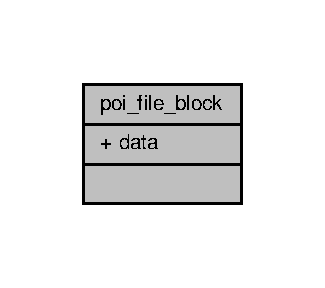
\includegraphics[width=156pt]{structpoi__file__block__coll__graph}
\end{center}
\end{figure}
\subsection*{Data Fields}
\begin{DoxyCompactItemize}
\item 
uint8\-\_\-t \hyperlink{structpoi__file__block_a453580bb9858958a75d49cd9a450a4b3}{data} \mbox{[}\hyperlink{file-manager_8h_afb59af7070cf0cd010913eef940ffbbd}{P\-O\-I\-\_\-\-B\-L\-O\-C\-K\-\_\-\-S\-I\-Z\-E}\mbox{]}
\end{DoxyCompactItemize}


\subsection{Field Documentation}
\hypertarget{structpoi__file__block_a453580bb9858958a75d49cd9a450a4b3}{\index{poi\-\_\-file\-\_\-block@{poi\-\_\-file\-\_\-block}!data@{data}}
\index{data@{data}!poi_file_block@{poi\-\_\-file\-\_\-block}}
\subsubsection[{data}]{\setlength{\rightskip}{0pt plus 5cm}uint8\-\_\-t data\mbox{[}{\bf P\-O\-I\-\_\-\-B\-L\-O\-C\-K\-\_\-\-S\-I\-Z\-E}\mbox{]}}}\label{structpoi__file__block_a453580bb9858958a75d49cd9a450a4b3}


The documentation for this struct was generated from the following file\-:\begin{DoxyCompactItemize}
\item 
src/\hyperlink{file-manager_8h}{file-\/manager.\-h}\end{DoxyCompactItemize}

\chapter{File Documentation}
\hypertarget{allocation-block-manager-test_8c}{\section{src/allocation-\/block-\/manager-\/test.c File Reference}
\label{allocation-block-manager-test_8c}\index{src/allocation-\/block-\/manager-\/test.\-c@{src/allocation-\/block-\/manager-\/test.\-c}}
}
{\ttfamily \#include \char`\"{}allocation-\/block-\/manager.\-h\char`\"{}}\\*
{\ttfamily \#include $<$assert.\-h$>$}\\*
Include dependency graph for allocation-\/block-\/manager-\/test.c\-:
\nopagebreak
\begin{figure}[H]
\begin{center}
\leavevmode
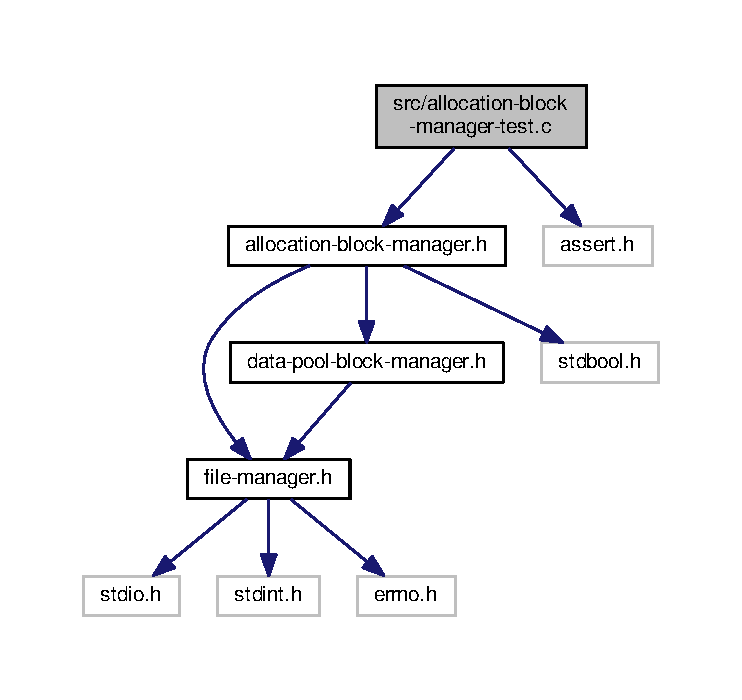
\includegraphics[width=350pt]{allocation-block-manager-test_8c__incl}
\end{center}
\end{figure}
\subsection*{Functions}
\begin{DoxyCompactItemize}
\item 
int \hyperlink{allocation-block-manager-test_8c_ae66f6b31b5ad750f1fe042a706a4e3d4}{main} ()
\end{DoxyCompactItemize}


\subsection{Function Documentation}
\hypertarget{allocation-block-manager-test_8c_ae66f6b31b5ad750f1fe042a706a4e3d4}{\index{allocation-\/block-\/manager-\/test.\-c@{allocation-\/block-\/manager-\/test.\-c}!main@{main}}
\index{main@{main}!allocation-block-manager-test.c@{allocation-\/block-\/manager-\/test.\-c}}
\subsubsection[{main}]{\setlength{\rightskip}{0pt plus 5cm}int main (
\begin{DoxyParamCaption}
{}
\end{DoxyParamCaption}
)}}\label{allocation-block-manager-test_8c_ae66f6b31b5ad750f1fe042a706a4e3d4}


Definition at line 4 of file allocation-\/block-\/manager-\/test.\-c.



Here is the call graph for this function\-:
\nopagebreak
\begin{figure}[H]
\begin{center}
\leavevmode
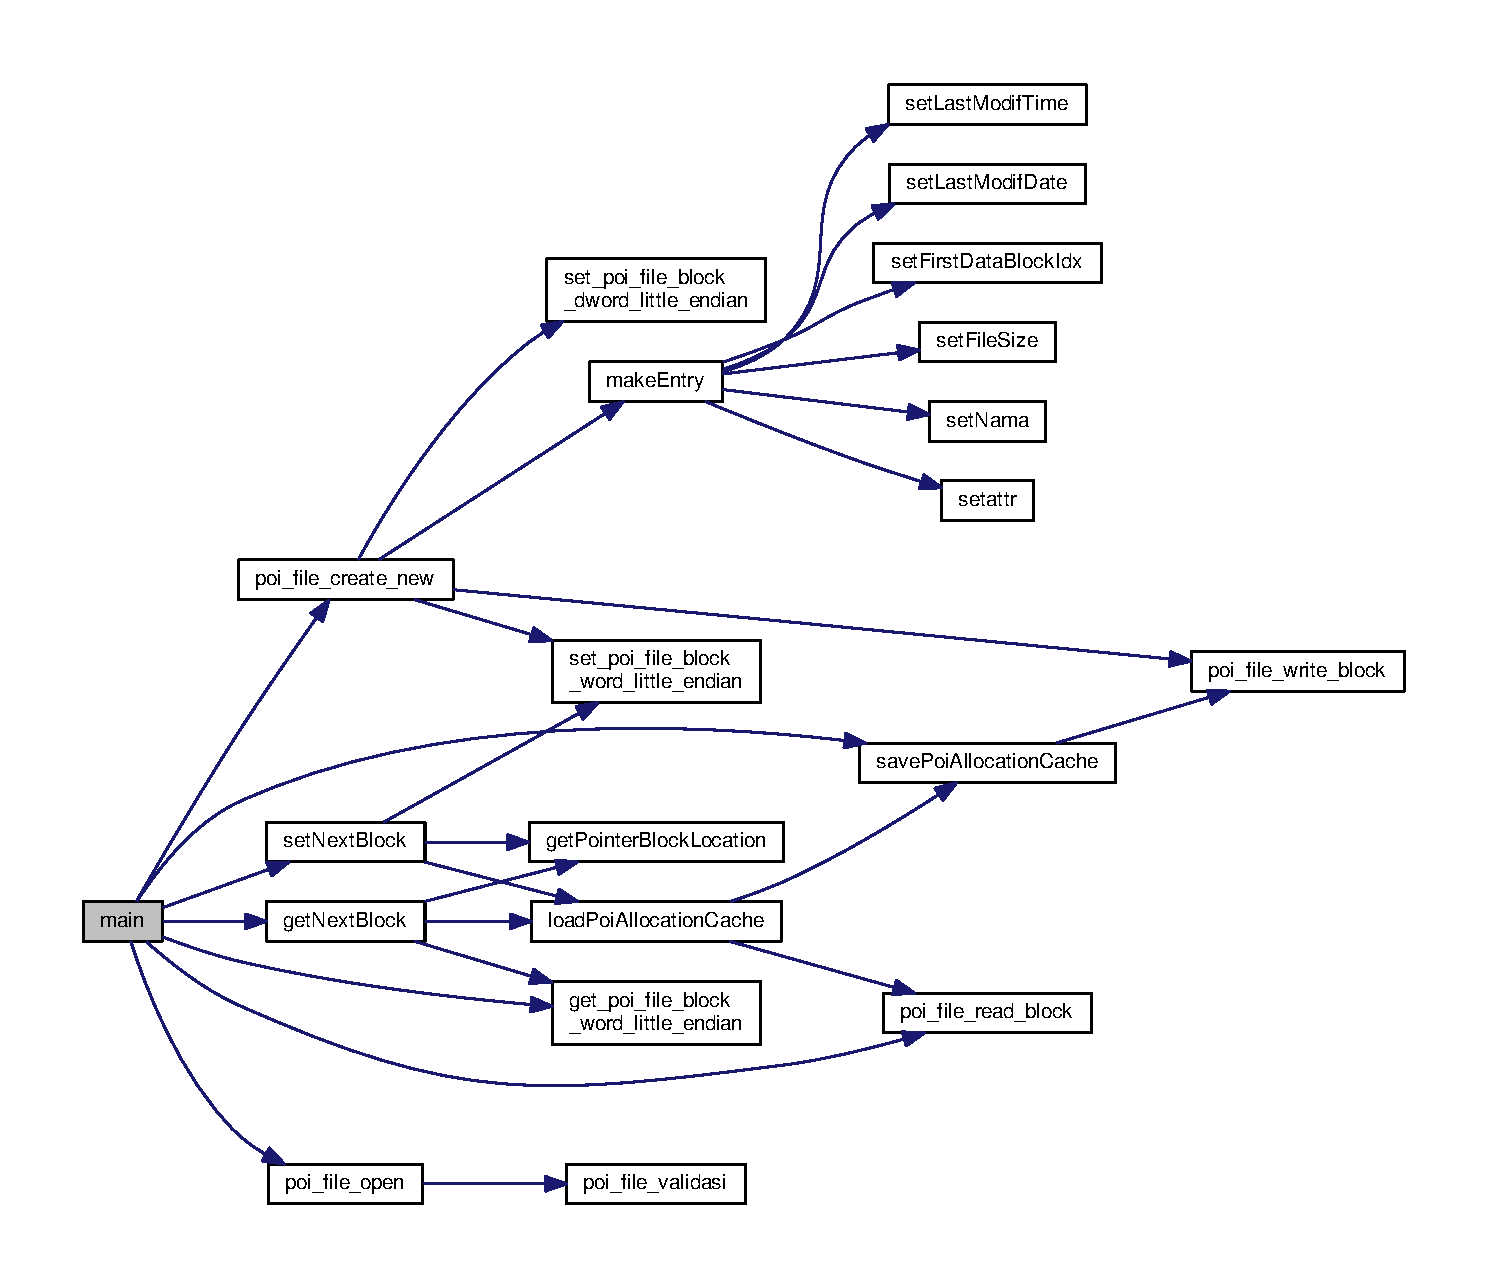
\includegraphics[width=350pt]{allocation-block-manager-test_8c_ae66f6b31b5ad750f1fe042a706a4e3d4_cgraph}
\end{center}
\end{figure}



\hypertarget{allocation-block-manager_8c}{\section{src/allocation-\/block-\/manager.c File Reference}
\label{allocation-block-manager_8c}\index{src/allocation-\/block-\/manager.\-c@{src/allocation-\/block-\/manager.\-c}}
}


mengambil dan menyimpan pointer to next di allocation table.  


{\ttfamily \#include \char`\"{}allocation-\/block-\/manager.\-h\char`\"{}}\\*
{\ttfamily \#include $<$assert.\-h$>$}\\*
Include dependency graph for allocation-\/block-\/manager.c\-:\nopagebreak
\begin{figure}[H]
\begin{center}
\leavevmode
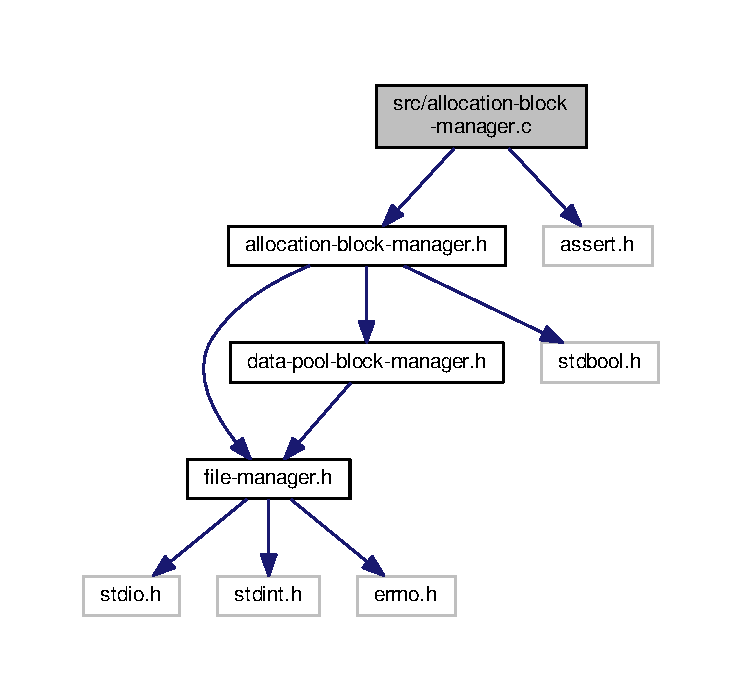
\includegraphics[width=350pt]{allocation-block-manager_8c__incl}
\end{center}
\end{figure}
\subsection*{Macros}
\begin{DoxyCompactItemize}
\item 
\#define \hyperlink{allocation-block-manager_8c_a7c27d1e5590b712625952d2abcef87f2}{allocation\-\_\-manager\-\_\-c}
\end{DoxyCompactItemize}
\subsection*{Functions}
\begin{DoxyCompactItemize}
\item 
void \hyperlink{allocation-block-manager_8c_a2d77f886ffa0a0d025a6a521cc6cf294}{load\-Poi\-Allocation\-Cache} (\hyperlink{file-manager_8h_aef709af8fc6566dcaf55b656bb9f8881}{poi\-\_\-file\-\_\-block\-\_\-num\-\_\-t} \hyperlink{allocation-table-test_8c_a24010dade8ebab3f87a48022772cd975}{n})
\item 
void \hyperlink{allocation-block-manager_8c_aa62c7923af0be489b52b1dcdd7c04e23}{save\-Poi\-Allocation\-Cache} ()
\item 
bool \hyperlink{allocation-block-manager_8c_a4b553c2a61827a60738c9323e6082903}{is\-Empty} (\hyperlink{data-pool-block-manager_8h_a87e19ab8290bcd76be1c7db1e90cc6f6}{poi\-\_\-data\-\_\-pool\-\_\-block\-\_\-idx\-\_\-t} \hyperlink{allocation-table-test_8c_a24010dade8ebab3f87a48022772cd975}{n})
\item 
\hyperlink{file-manager_8h_aef709af8fc6566dcaf55b656bb9f8881}{poi\-\_\-file\-\_\-block\-\_\-num\-\_\-t} \hyperlink{allocation-block-manager_8c_a451dec2ee6d7a7241ab5fbc0a2ad0259}{get\-Pointer\-Block\-Location} (\hyperlink{data-pool-block-manager_8h_a87e19ab8290bcd76be1c7db1e90cc6f6}{poi\-\_\-data\-\_\-pool\-\_\-block\-\_\-idx\-\_\-t} \hyperlink{allocation-table-test_8c_a24010dade8ebab3f87a48022772cd975}{n})
\item 
\hyperlink{data-pool-block-manager_8h_a87e19ab8290bcd76be1c7db1e90cc6f6}{poi\-\_\-data\-\_\-pool\-\_\-block\-\_\-idx\-\_\-t} \hyperlink{allocation-block-manager_8c_a0843a74a7e1cc7c50dbfa521e4ea1cc8}{get\-Next\-Block} (\hyperlink{data-pool-block-manager_8h_a87e19ab8290bcd76be1c7db1e90cc6f6}{poi\-\_\-data\-\_\-pool\-\_\-block\-\_\-idx\-\_\-t} \hyperlink{allocation-table-test_8c_a24010dade8ebab3f87a48022772cd975}{n})
\item 
void \hyperlink{allocation-block-manager_8c_a7387272862663d2af1af9d5c21cddc84}{set\-Next\-Block} (\hyperlink{data-pool-block-manager_8h_a87e19ab8290bcd76be1c7db1e90cc6f6}{poi\-\_\-data\-\_\-pool\-\_\-block\-\_\-idx\-\_\-t} current, \hyperlink{data-pool-block-manager_8h_a87e19ab8290bcd76be1c7db1e90cc6f6}{poi\-\_\-data\-\_\-pool\-\_\-block\-\_\-idx\-\_\-t} next)
\item 
\hyperlink{data-pool-block-manager_8h_a87e19ab8290bcd76be1c7db1e90cc6f6}{poi\-\_\-data\-\_\-pool\-\_\-block\-\_\-idx\-\_\-t} \hyperlink{allocation-block-manager_8c_ab352dc84382d70f0044e92c52165c2cc}{get\-Next\-Empty} (\hyperlink{data-pool-block-manager_8h_a87e19ab8290bcd76be1c7db1e90cc6f6}{poi\-\_\-data\-\_\-pool\-\_\-block\-\_\-idx\-\_\-t} \hyperlink{allocation-table-test_8c_a24010dade8ebab3f87a48022772cd975}{n})
\end{DoxyCompactItemize}
\subsection*{Variables}
\begin{DoxyCompactItemize}
\item 
\hyperlink{structpoi__file__block}{poi\-\_\-file\-\_\-block} \hyperlink{allocation-block-manager_8c_a8cca9731003c6880e9aa8c3eb9d24951}{poi\-\_\-allocation\-\_\-cache}
\item 
int \hyperlink{allocation-block-manager_8c_a0f8b81672add5e3cee6cadcec0ff91b6}{poi\-\_\-allocation\-\_\-cache\-\_\-file\-\_\-block\-\_\-num} = 0
\end{DoxyCompactItemize}


\subsection{Detailed Description}
mengambil dan menyimpan pointer to next di allocation table. \begin{DoxyAuthor}{Author}
jang berikoetnja Tidak memperhitungkan free space. Memiliki cache. Setiap akhir manipulasi harus memanggil \hyperlink{allocation-block-manager_8c_aa62c7923af0be489b52b1dcdd7c04e23}{save\-Poi\-Allocation\-Cache()} 
\end{DoxyAuthor}


\subsection{Macro Definition Documentation}
\hypertarget{allocation-block-manager_8c_a7c27d1e5590b712625952d2abcef87f2}{\index{allocation-\/block-\/manager.\-c@{allocation-\/block-\/manager.\-c}!allocation\-\_\-manager\-\_\-c@{allocation\-\_\-manager\-\_\-c}}
\index{allocation\-\_\-manager\-\_\-c@{allocation\-\_\-manager\-\_\-c}!allocation-block-manager.c@{allocation-\/block-\/manager.\-c}}
\subsubsection[{allocation\-\_\-manager\-\_\-c}]{\setlength{\rightskip}{0pt plus 5cm}\#define allocation\-\_\-manager\-\_\-c}}\label{allocation-block-manager_8c_a7c27d1e5590b712625952d2abcef87f2}


\subsection{Function Documentation}
\hypertarget{allocation-block-manager_8c_a0843a74a7e1cc7c50dbfa521e4ea1cc8}{\index{allocation-\/block-\/manager.\-c@{allocation-\/block-\/manager.\-c}!get\-Next\-Block@{get\-Next\-Block}}
\index{get\-Next\-Block@{get\-Next\-Block}!allocation-block-manager.c@{allocation-\/block-\/manager.\-c}}
\subsubsection[{get\-Next\-Block}]{\setlength{\rightskip}{0pt plus 5cm}{\bf poi\-\_\-data\-\_\-pool\-\_\-block\-\_\-idx\-\_\-t} get\-Next\-Block (
\begin{DoxyParamCaption}
\item[{{\bf poi\-\_\-data\-\_\-pool\-\_\-block\-\_\-idx\-\_\-t}}]{n}
\end{DoxyParamCaption}
)}}\label{allocation-block-manager_8c_a0843a74a7e1cc7c50dbfa521e4ea1cc8}


Here is the call graph for this function\-:\nopagebreak
\begin{figure}[H]
\begin{center}
\leavevmode
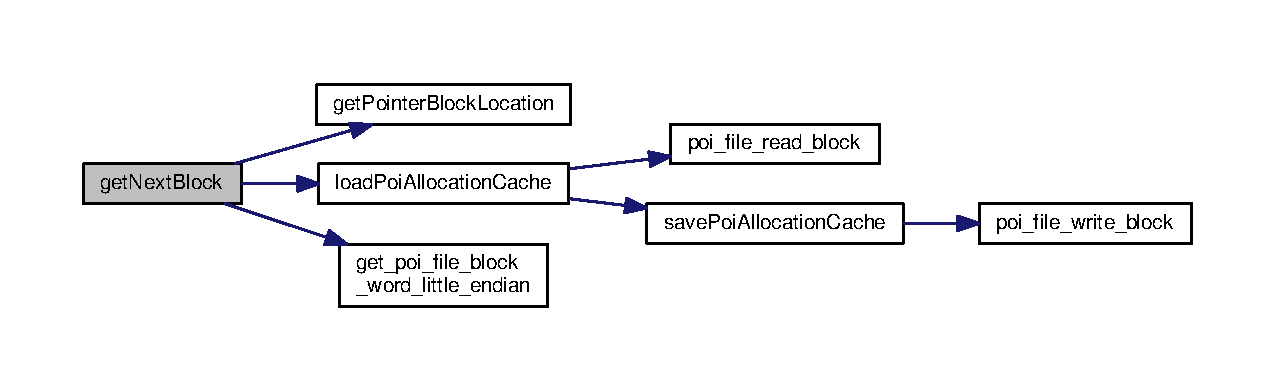
\includegraphics[width=350pt]{allocation-block-manager_8c_a0843a74a7e1cc7c50dbfa521e4ea1cc8_cgraph}
\end{center}
\end{figure}




Here is the caller graph for this function\-:
\nopagebreak
\begin{figure}[H]
\begin{center}
\leavevmode
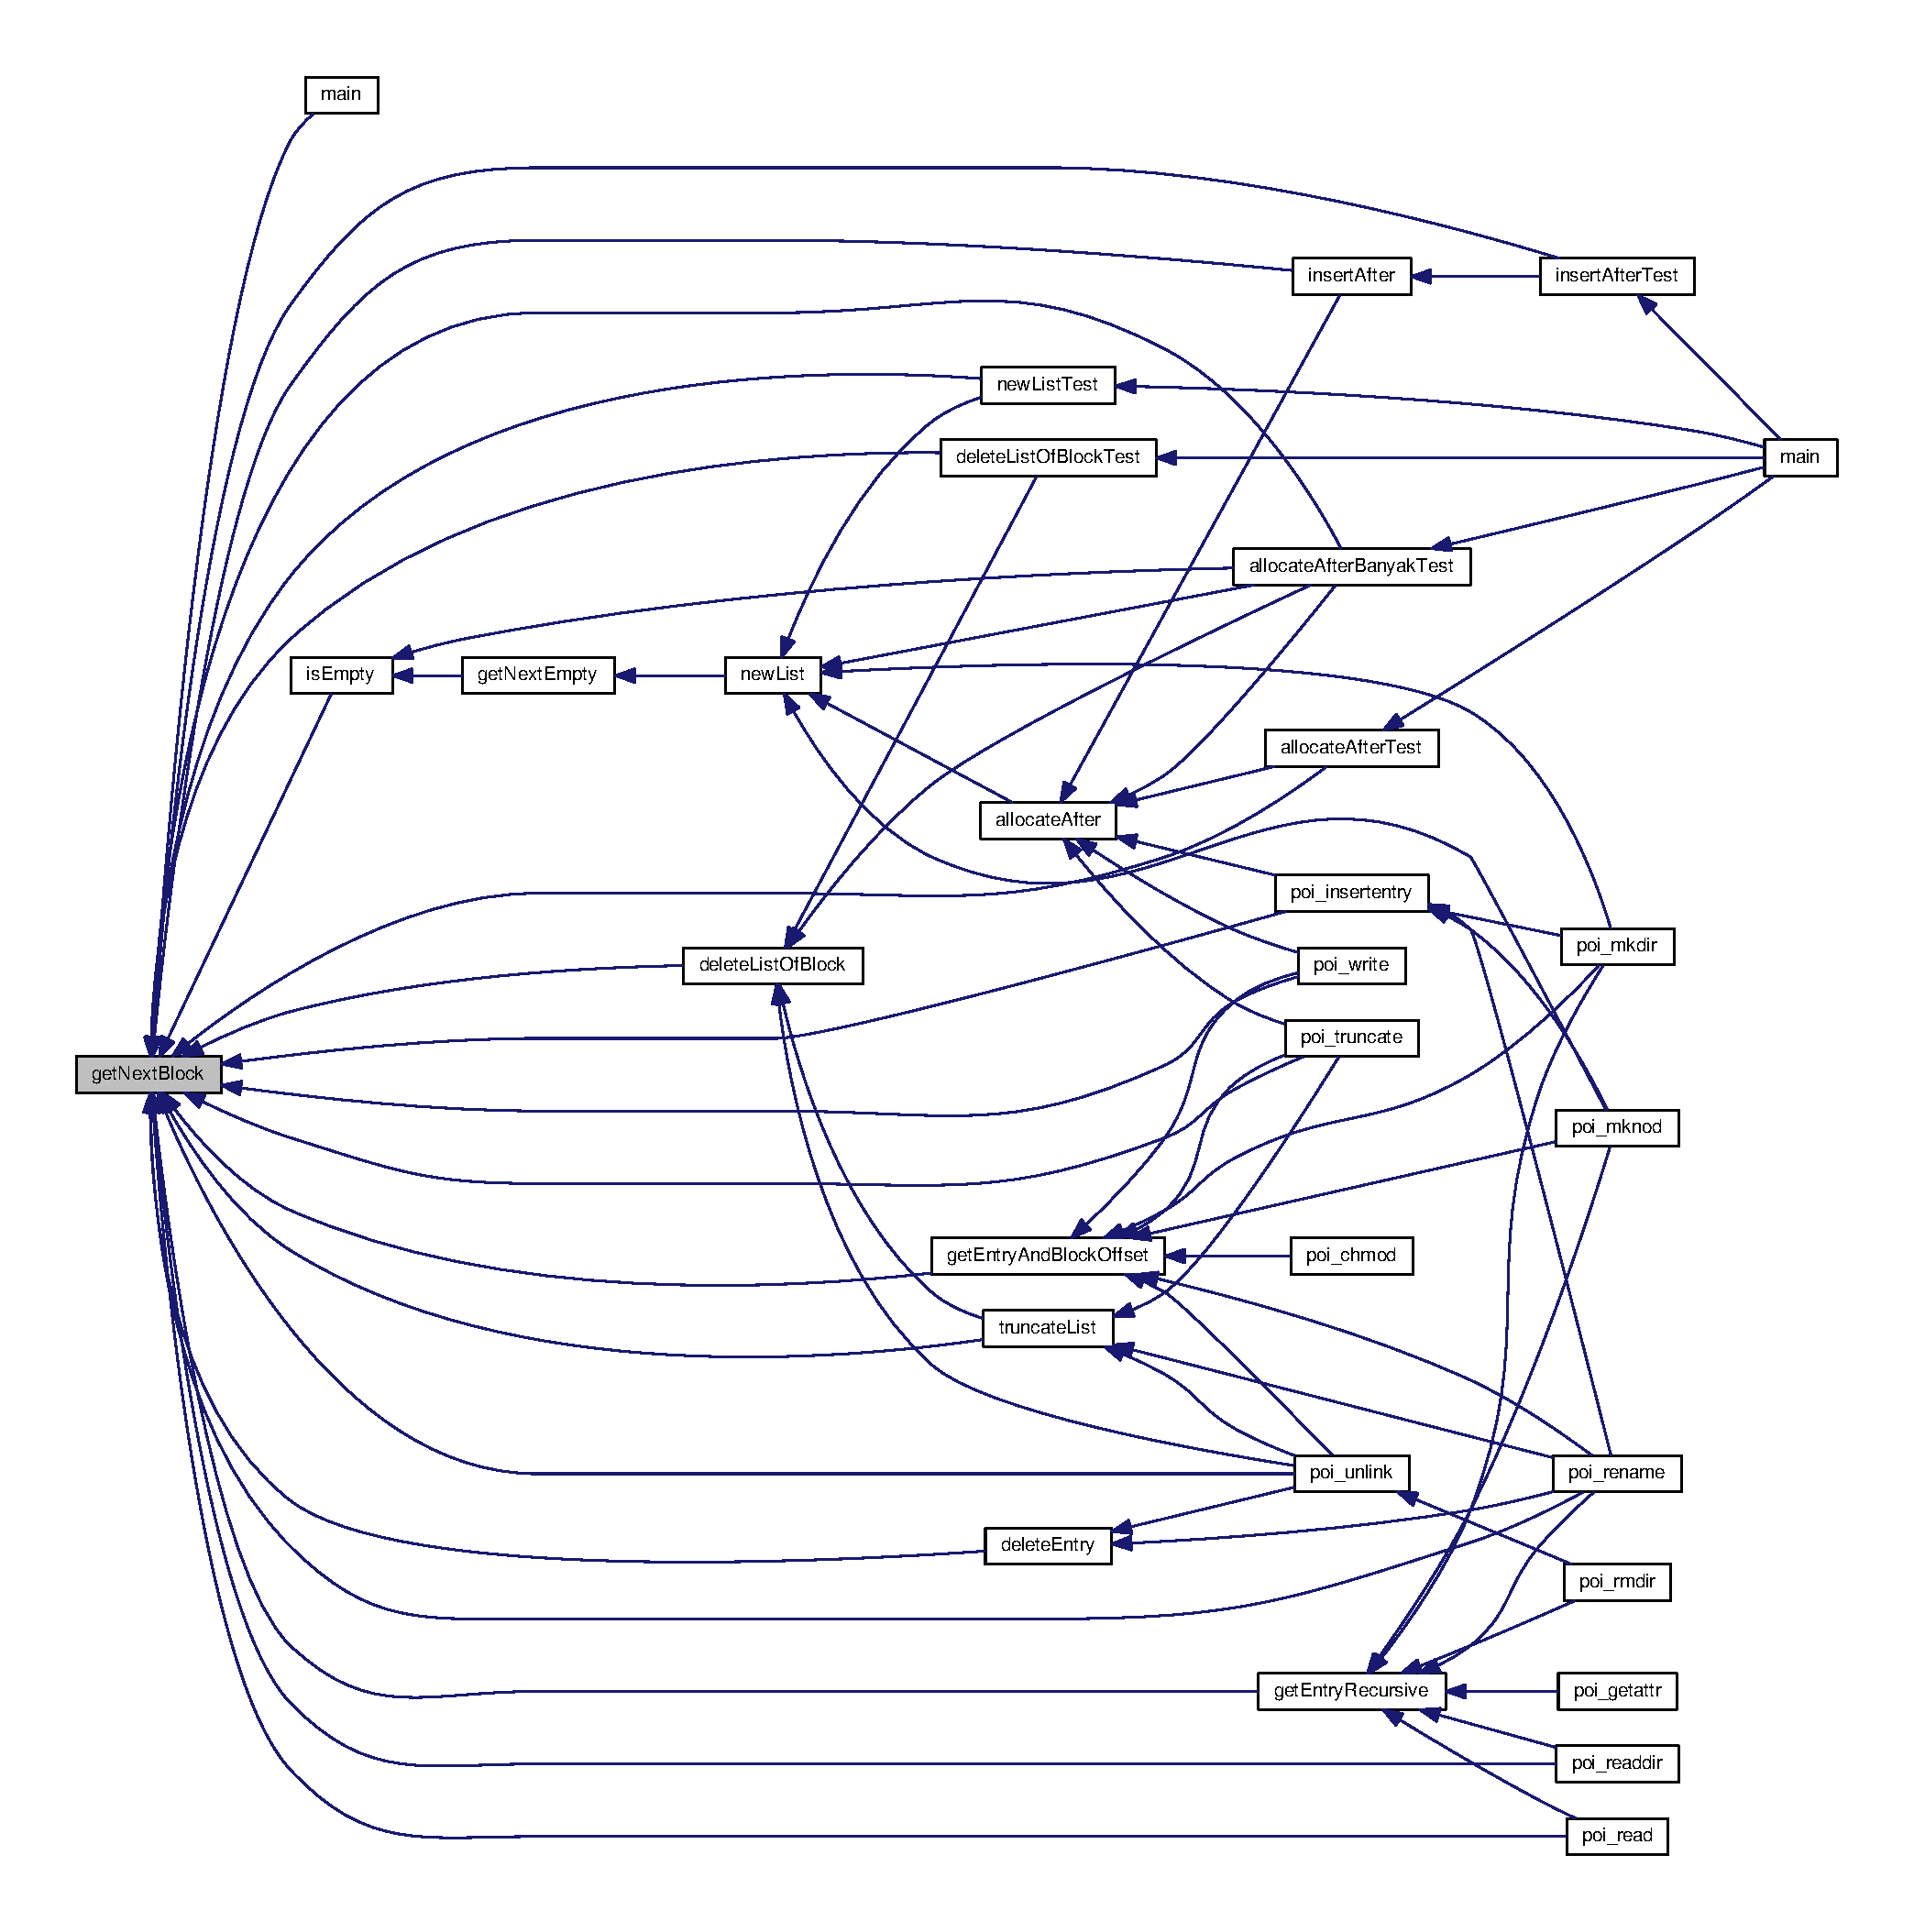
\includegraphics[width=350pt]{allocation-block-manager_8c_a0843a74a7e1cc7c50dbfa521e4ea1cc8_icgraph}
\end{center}
\end{figure}


\hypertarget{allocation-block-manager_8c_ab352dc84382d70f0044e92c52165c2cc}{\index{allocation-\/block-\/manager.\-c@{allocation-\/block-\/manager.\-c}!get\-Next\-Empty@{get\-Next\-Empty}}
\index{get\-Next\-Empty@{get\-Next\-Empty}!allocation-block-manager.c@{allocation-\/block-\/manager.\-c}}
\subsubsection[{get\-Next\-Empty}]{\setlength{\rightskip}{0pt plus 5cm}{\bf poi\-\_\-data\-\_\-pool\-\_\-block\-\_\-idx\-\_\-t} get\-Next\-Empty (
\begin{DoxyParamCaption}
\item[{{\bf poi\-\_\-data\-\_\-pool\-\_\-block\-\_\-idx\-\_\-t}}]{n}
\end{DoxyParamCaption}
)}}\label{allocation-block-manager_8c_ab352dc84382d70f0044e92c52165c2cc}


Here is the call graph for this function\-:\nopagebreak
\begin{figure}[H]
\begin{center}
\leavevmode
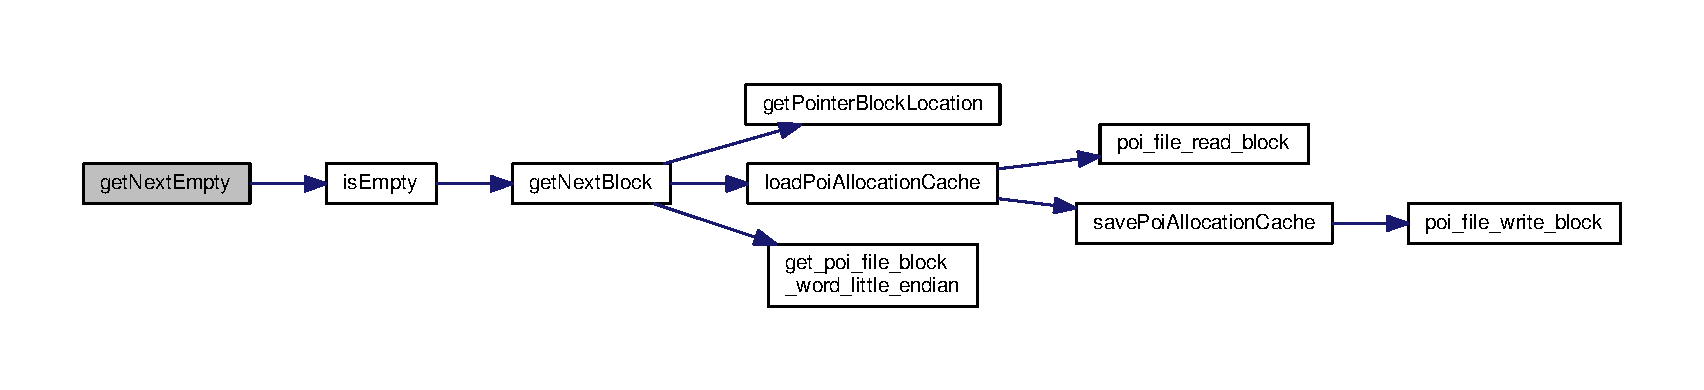
\includegraphics[width=350pt]{allocation-block-manager_8c_ab352dc84382d70f0044e92c52165c2cc_cgraph}
\end{center}
\end{figure}




Here is the caller graph for this function\-:\nopagebreak
\begin{figure}[H]
\begin{center}
\leavevmode
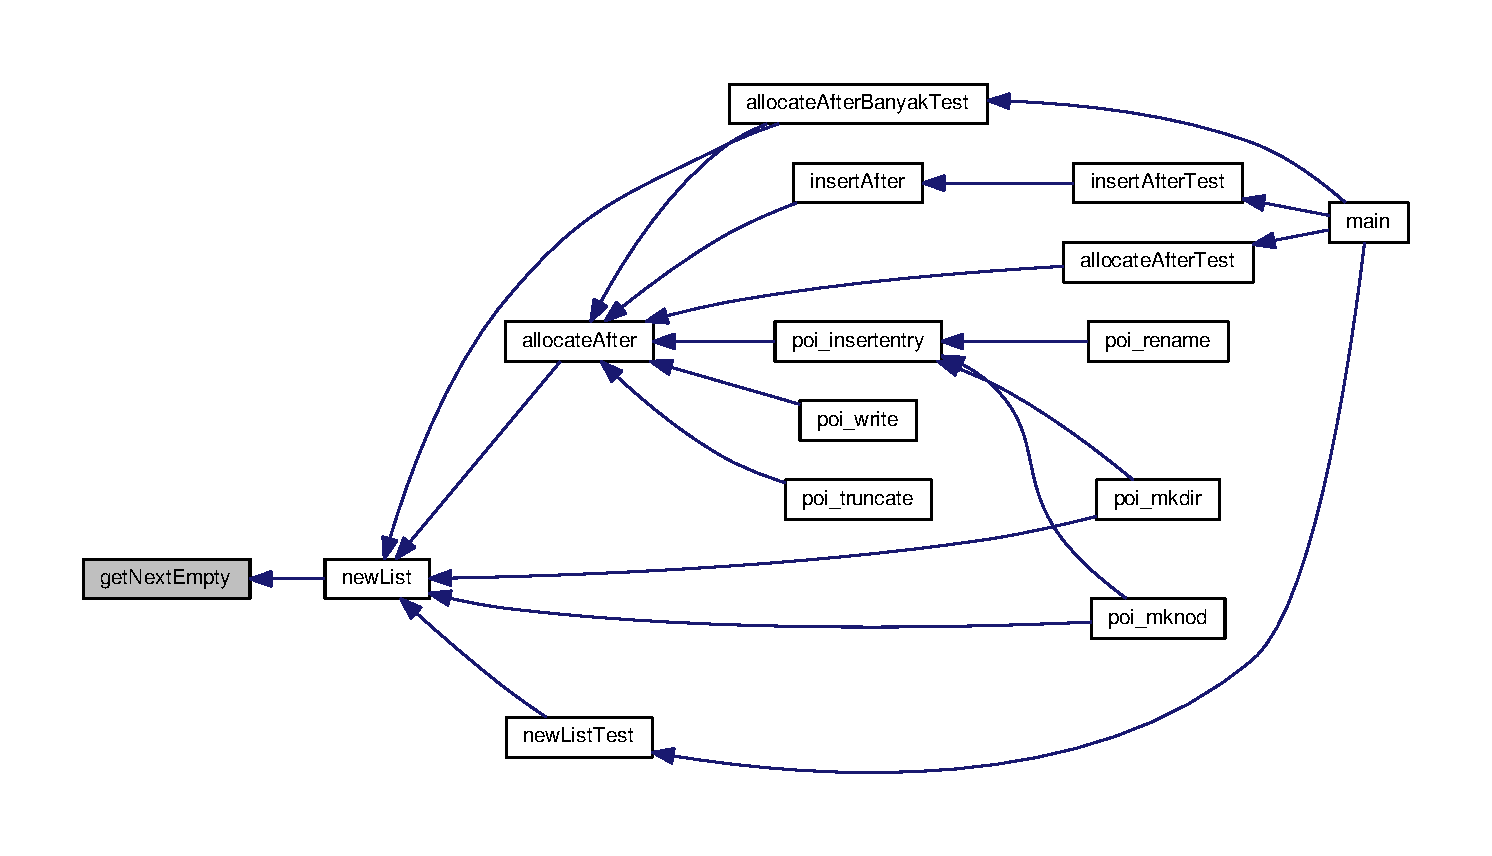
\includegraphics[width=350pt]{allocation-block-manager_8c_ab352dc84382d70f0044e92c52165c2cc_icgraph}
\end{center}
\end{figure}


\hypertarget{allocation-block-manager_8c_a451dec2ee6d7a7241ab5fbc0a2ad0259}{\index{allocation-\/block-\/manager.\-c@{allocation-\/block-\/manager.\-c}!get\-Pointer\-Block\-Location@{get\-Pointer\-Block\-Location}}
\index{get\-Pointer\-Block\-Location@{get\-Pointer\-Block\-Location}!allocation-block-manager.c@{allocation-\/block-\/manager.\-c}}
\subsubsection[{get\-Pointer\-Block\-Location}]{\setlength{\rightskip}{0pt plus 5cm}{\bf poi\-\_\-file\-\_\-block\-\_\-num\-\_\-t} get\-Pointer\-Block\-Location (
\begin{DoxyParamCaption}
\item[{{\bf poi\-\_\-data\-\_\-pool\-\_\-block\-\_\-idx\-\_\-t}}]{n}
\end{DoxyParamCaption}
)}}\label{allocation-block-manager_8c_a451dec2ee6d7a7241ab5fbc0a2ad0259}


Here is the caller graph for this function\-:
\nopagebreak
\begin{figure}[H]
\begin{center}
\leavevmode
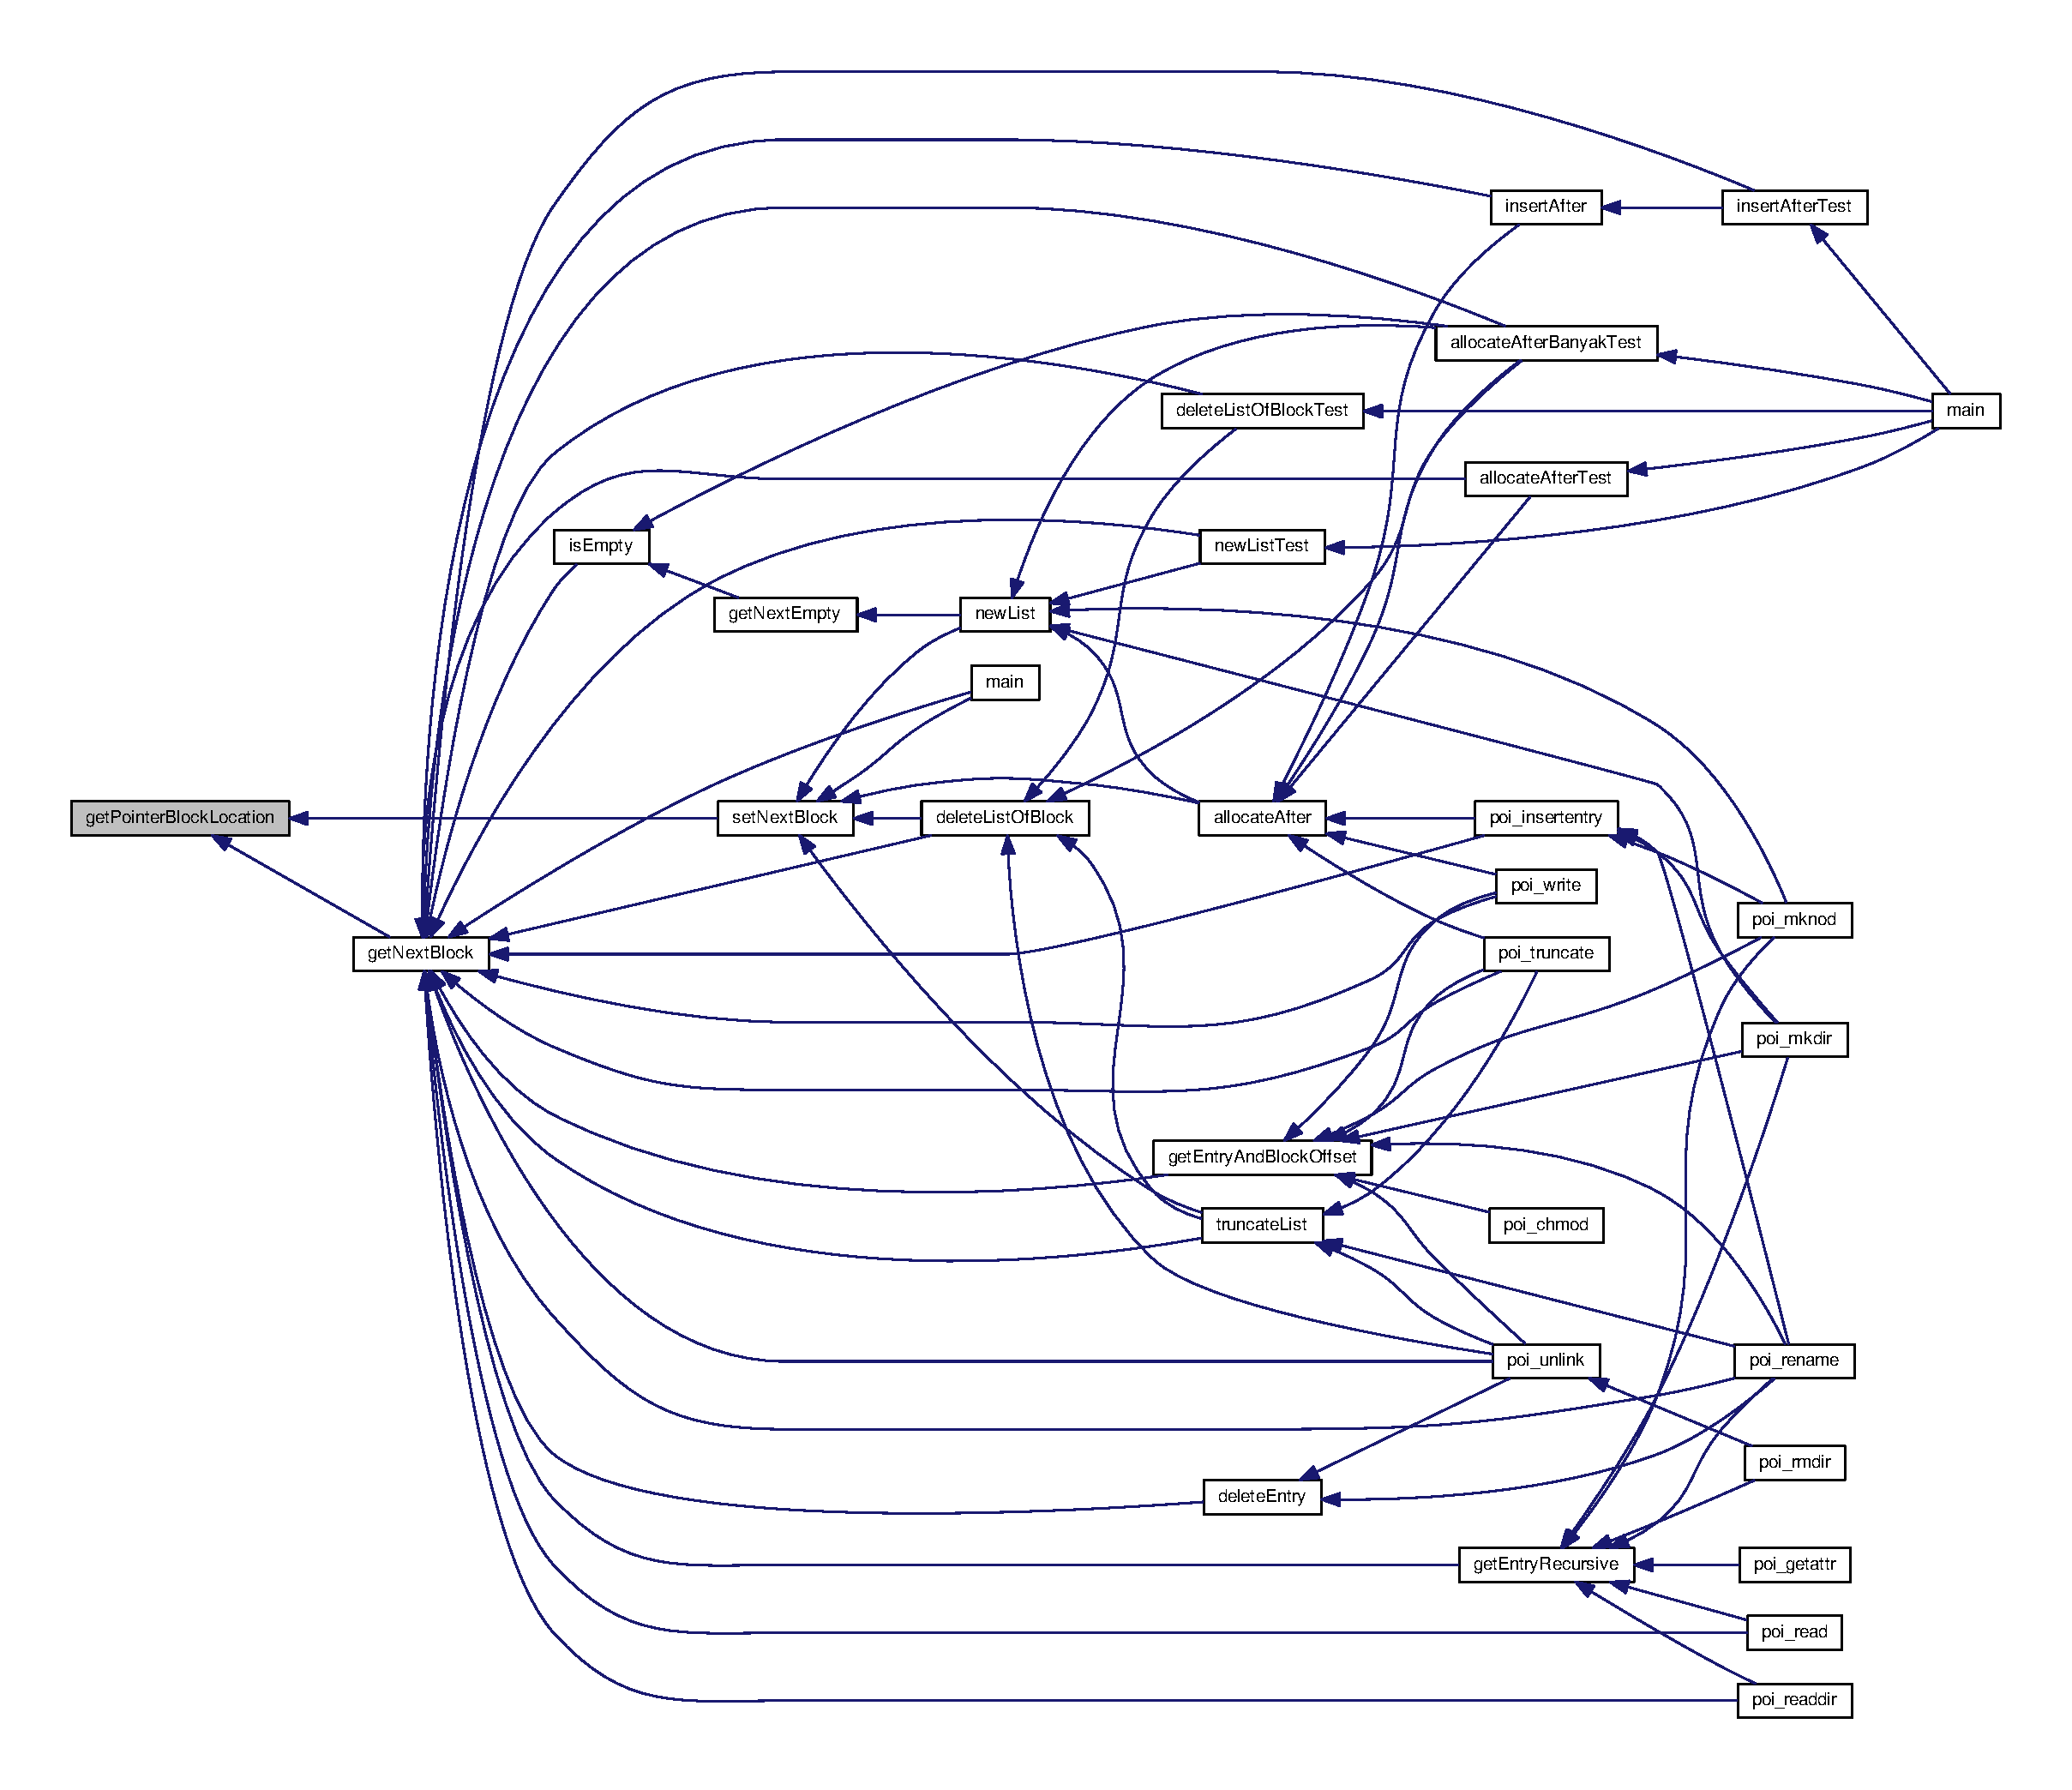
\includegraphics[width=350pt]{allocation-block-manager_8c_a451dec2ee6d7a7241ab5fbc0a2ad0259_icgraph}
\end{center}
\end{figure}


\hypertarget{allocation-block-manager_8c_a4b553c2a61827a60738c9323e6082903}{\index{allocation-\/block-\/manager.\-c@{allocation-\/block-\/manager.\-c}!is\-Empty@{is\-Empty}}
\index{is\-Empty@{is\-Empty}!allocation-block-manager.c@{allocation-\/block-\/manager.\-c}}
\subsubsection[{is\-Empty}]{\setlength{\rightskip}{0pt plus 5cm}bool is\-Empty (
\begin{DoxyParamCaption}
\item[{{\bf poi\-\_\-data\-\_\-pool\-\_\-block\-\_\-idx\-\_\-t}}]{n}
\end{DoxyParamCaption}
)}}\label{allocation-block-manager_8c_a4b553c2a61827a60738c9323e6082903}


Here is the call graph for this function\-:\nopagebreak
\begin{figure}[H]
\begin{center}
\leavevmode
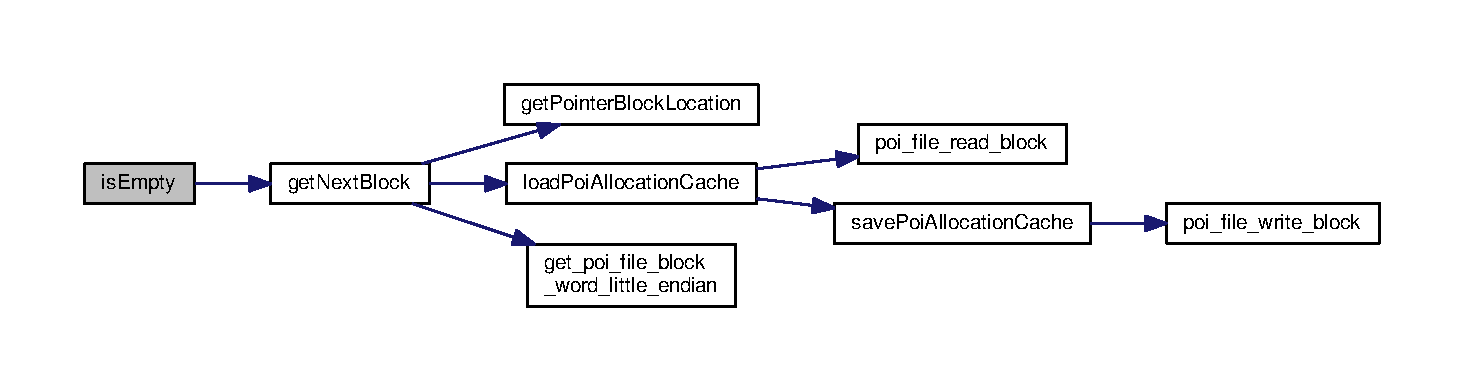
\includegraphics[width=350pt]{allocation-block-manager_8c_a4b553c2a61827a60738c9323e6082903_cgraph}
\end{center}
\end{figure}




Here is the caller graph for this function\-:\nopagebreak
\begin{figure}[H]
\begin{center}
\leavevmode
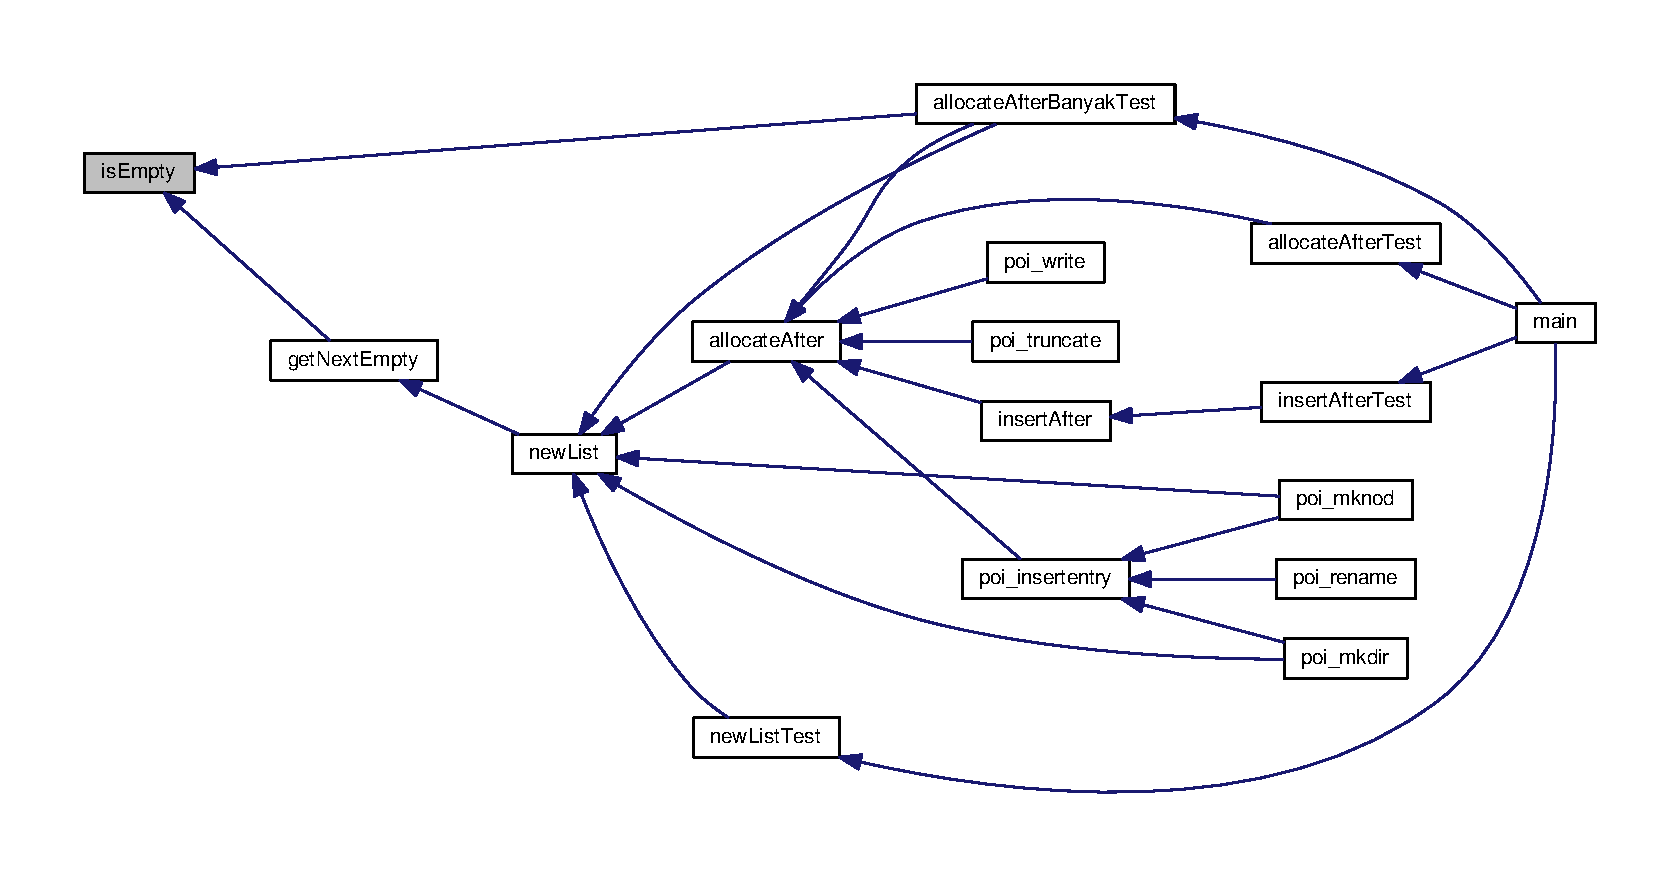
\includegraphics[width=350pt]{allocation-block-manager_8c_a4b553c2a61827a60738c9323e6082903_icgraph}
\end{center}
\end{figure}


\hypertarget{allocation-block-manager_8c_a2d77f886ffa0a0d025a6a521cc6cf294}{\index{allocation-\/block-\/manager.\-c@{allocation-\/block-\/manager.\-c}!load\-Poi\-Allocation\-Cache@{load\-Poi\-Allocation\-Cache}}
\index{load\-Poi\-Allocation\-Cache@{load\-Poi\-Allocation\-Cache}!allocation-block-manager.c@{allocation-\/block-\/manager.\-c}}
\subsubsection[{load\-Poi\-Allocation\-Cache}]{\setlength{\rightskip}{0pt plus 5cm}void load\-Poi\-Allocation\-Cache (
\begin{DoxyParamCaption}
\item[{{\bf poi\-\_\-file\-\_\-block\-\_\-num\-\_\-t}}]{n}
\end{DoxyParamCaption}
)}}\label{allocation-block-manager_8c_a2d77f886ffa0a0d025a6a521cc6cf294}


Here is the call graph for this function\-:\nopagebreak
\begin{figure}[H]
\begin{center}
\leavevmode
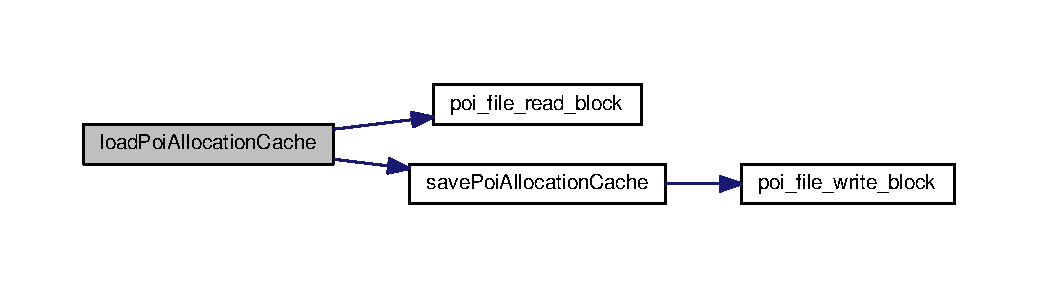
\includegraphics[width=350pt]{allocation-block-manager_8c_a2d77f886ffa0a0d025a6a521cc6cf294_cgraph}
\end{center}
\end{figure}




Here is the caller graph for this function\-:
\nopagebreak
\begin{figure}[H]
\begin{center}
\leavevmode
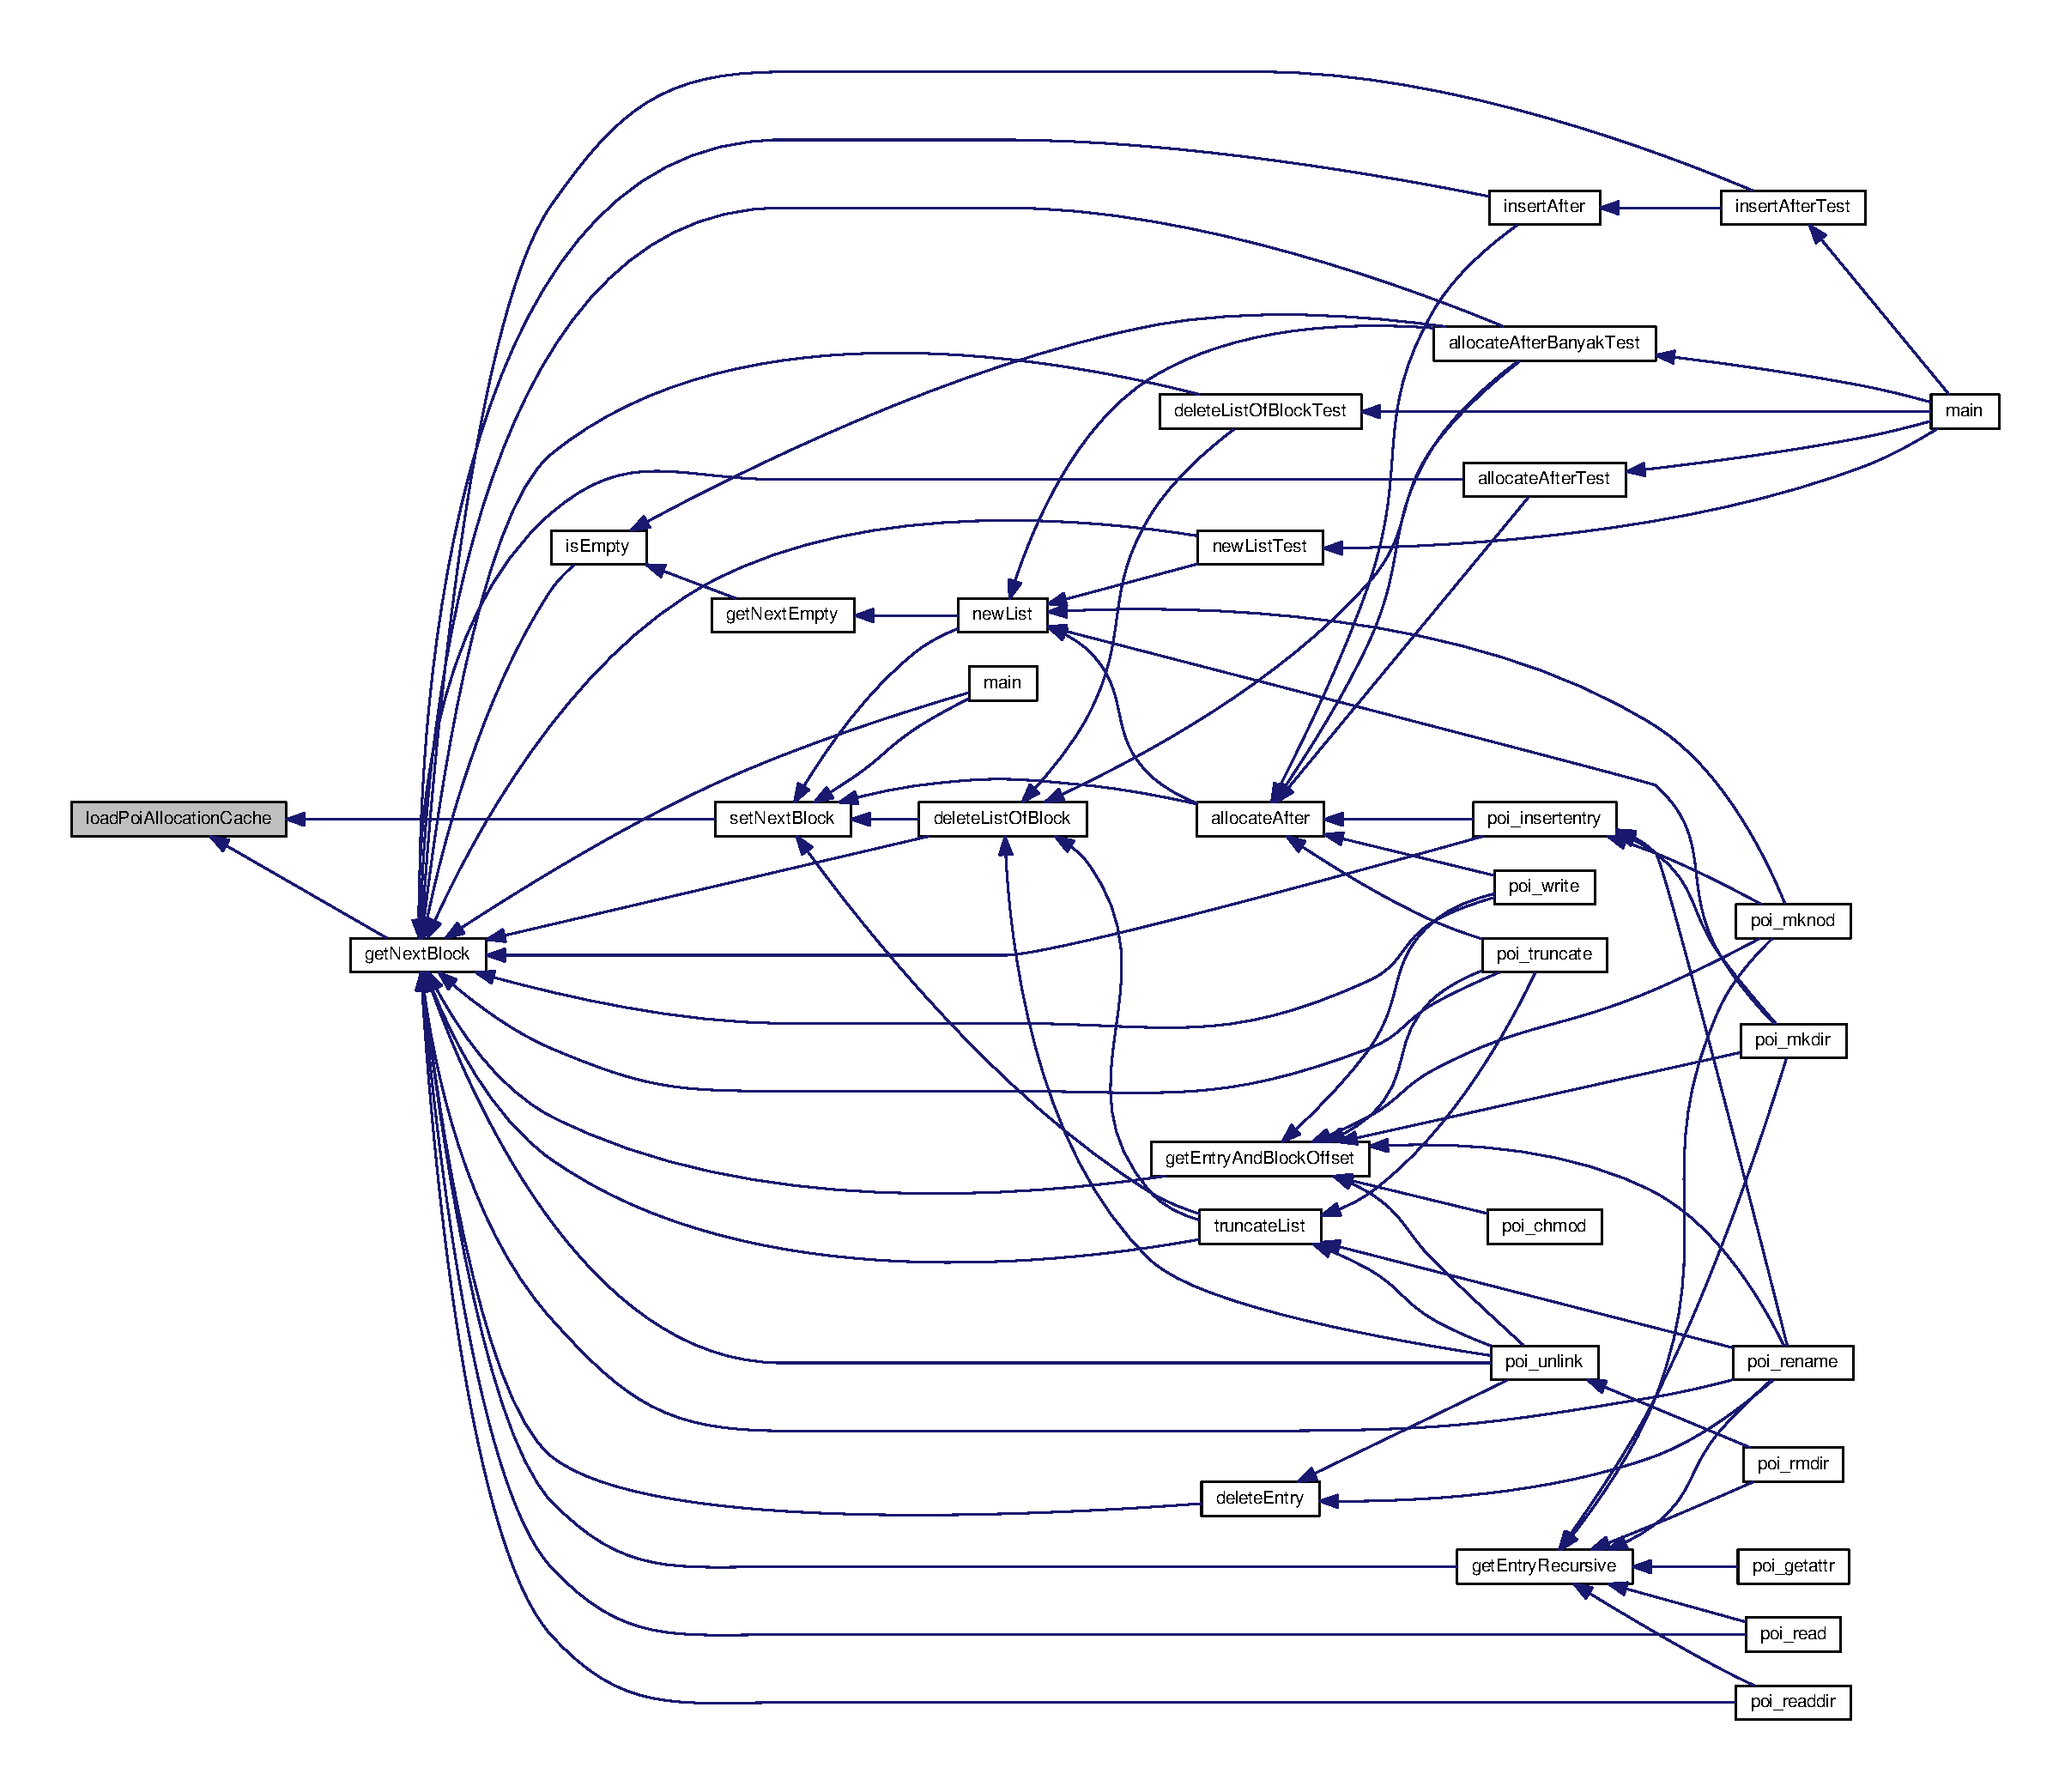
\includegraphics[width=350pt]{allocation-block-manager_8c_a2d77f886ffa0a0d025a6a521cc6cf294_icgraph}
\end{center}
\end{figure}


\hypertarget{allocation-block-manager_8c_aa62c7923af0be489b52b1dcdd7c04e23}{\index{allocation-\/block-\/manager.\-c@{allocation-\/block-\/manager.\-c}!save\-Poi\-Allocation\-Cache@{save\-Poi\-Allocation\-Cache}}
\index{save\-Poi\-Allocation\-Cache@{save\-Poi\-Allocation\-Cache}!allocation-block-manager.c@{allocation-\/block-\/manager.\-c}}
\subsubsection[{save\-Poi\-Allocation\-Cache}]{\setlength{\rightskip}{0pt plus 5cm}void save\-Poi\-Allocation\-Cache (
\begin{DoxyParamCaption}
{}
\end{DoxyParamCaption}
)}}\label{allocation-block-manager_8c_aa62c7923af0be489b52b1dcdd7c04e23}


Here is the call graph for this function\-:\nopagebreak
\begin{figure}[H]
\begin{center}
\leavevmode
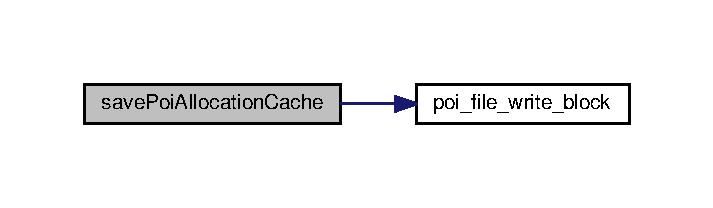
\includegraphics[width=342pt]{allocation-block-manager_8c_aa62c7923af0be489b52b1dcdd7c04e23_cgraph}
\end{center}
\end{figure}




Here is the caller graph for this function\-:
\nopagebreak
\begin{figure}[H]
\begin{center}
\leavevmode
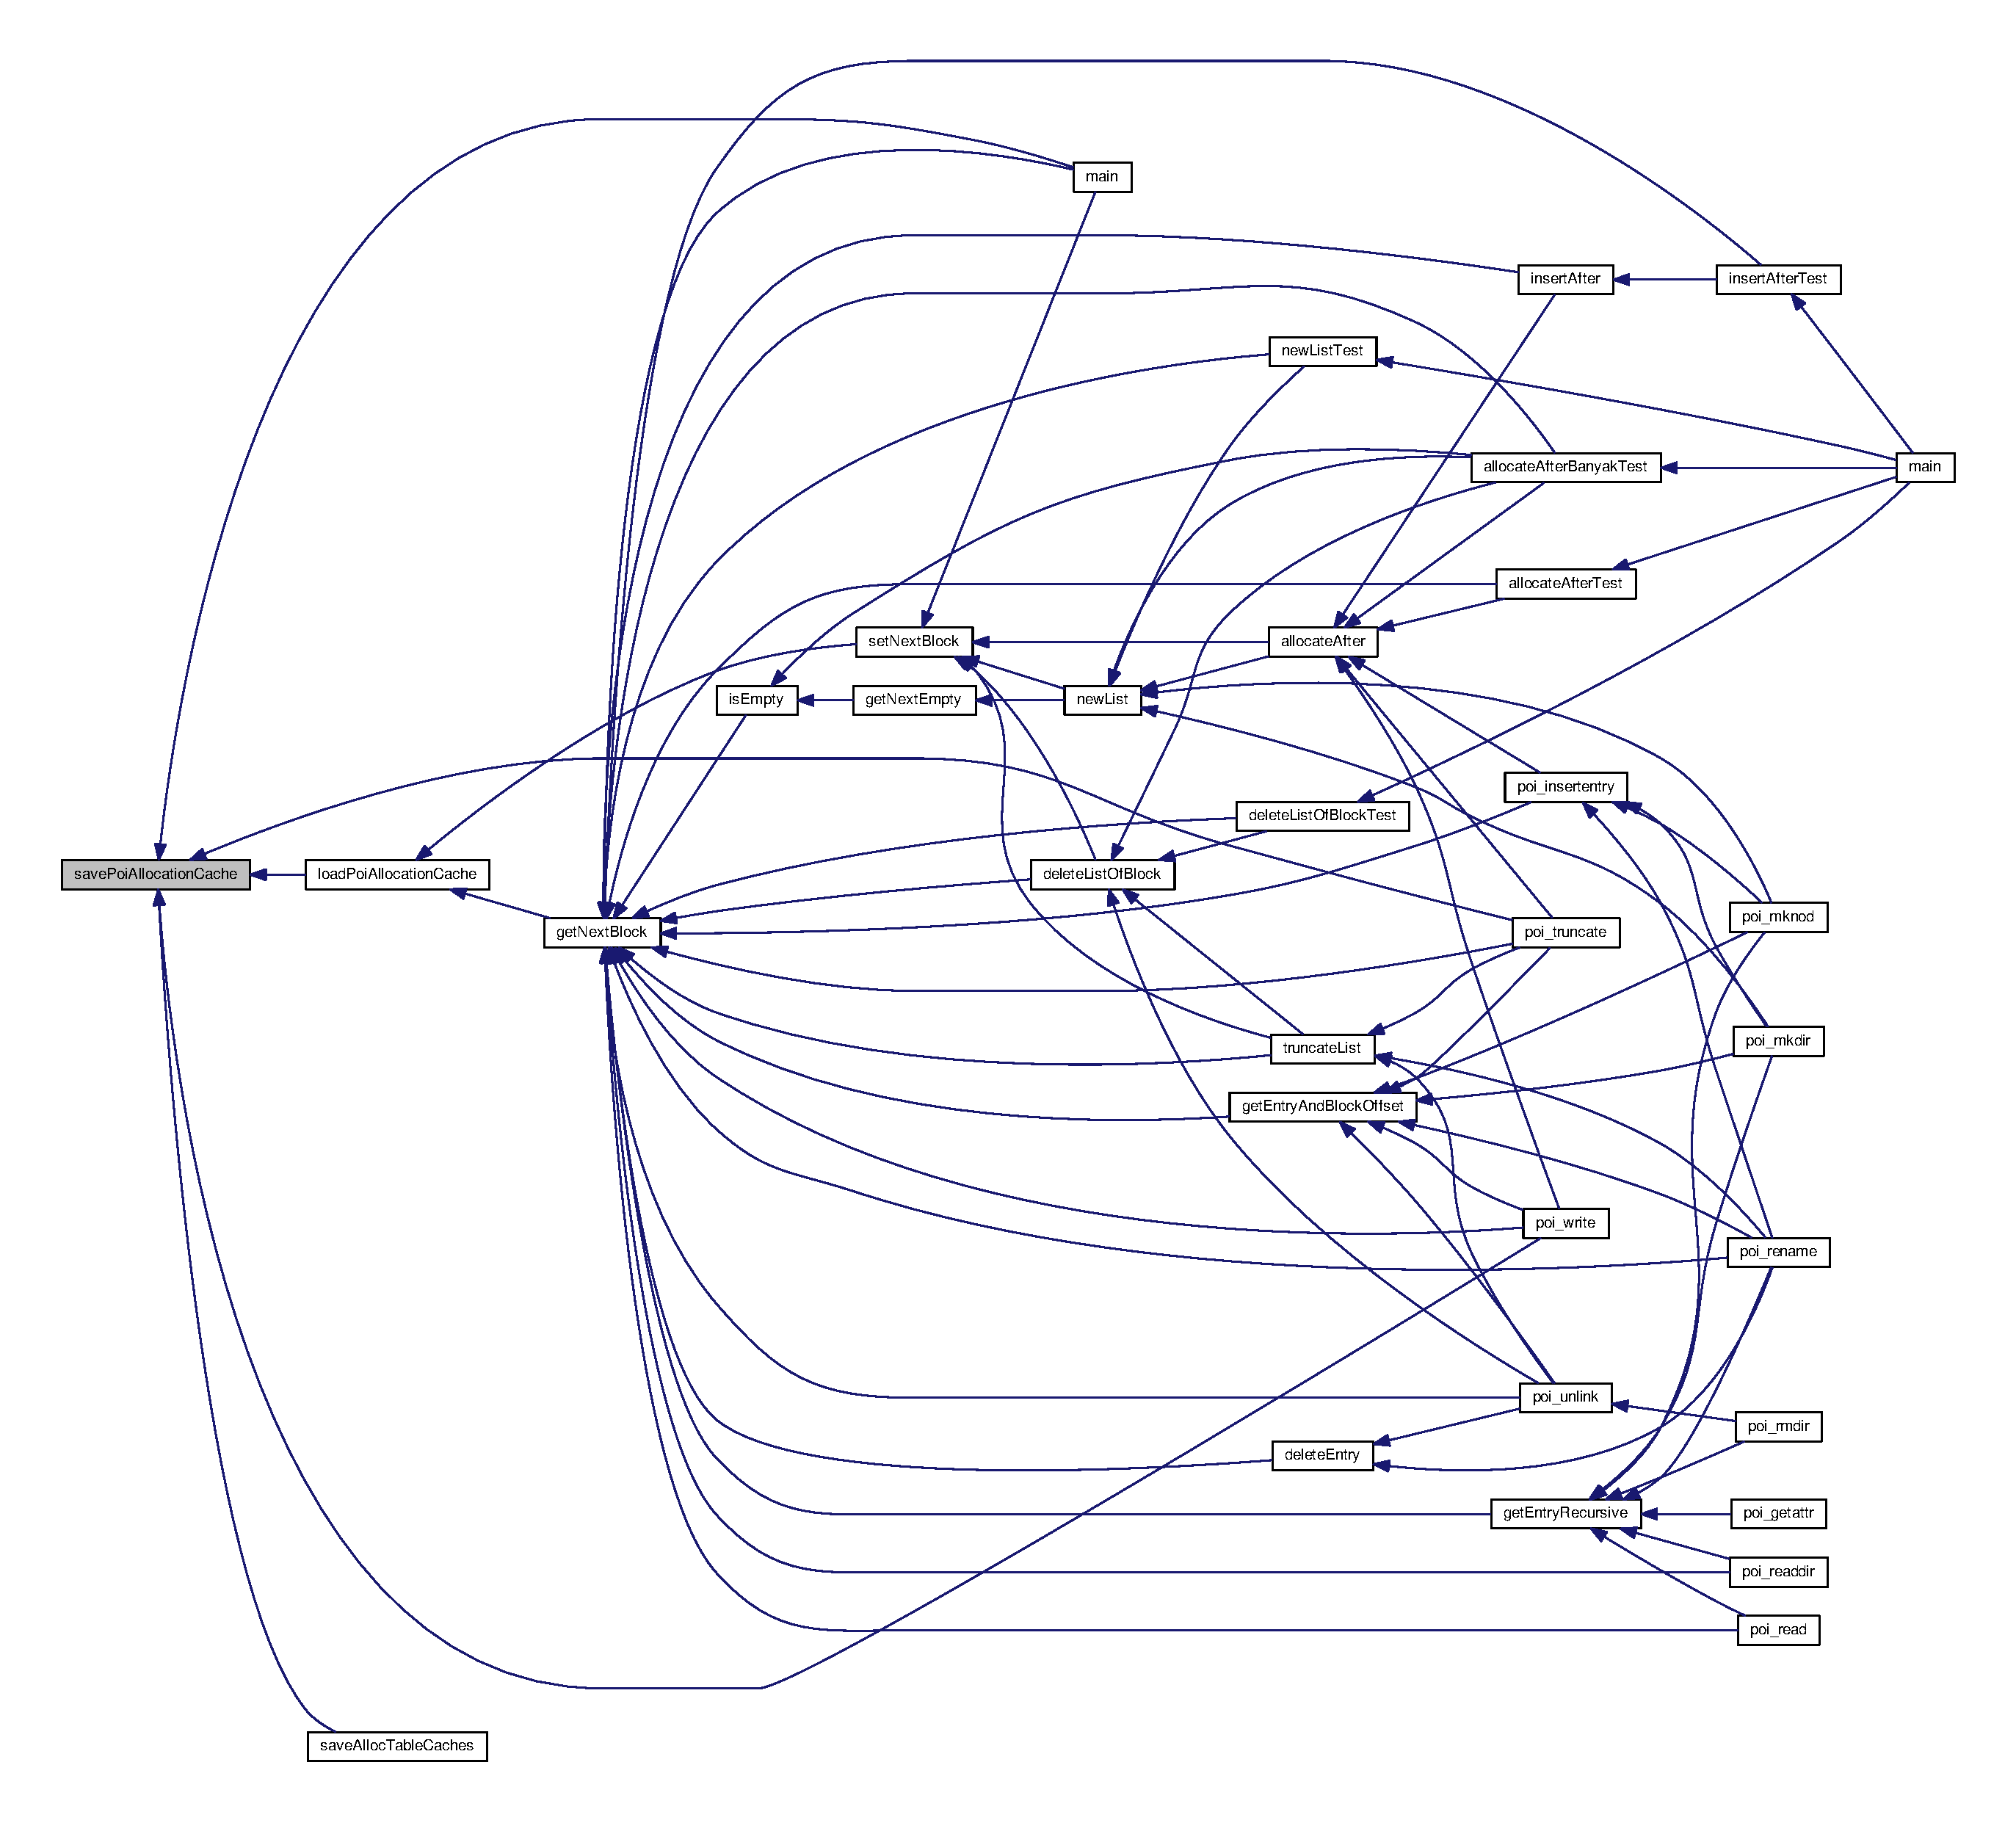
\includegraphics[width=350pt]{allocation-block-manager_8c_aa62c7923af0be489b52b1dcdd7c04e23_icgraph}
\end{center}
\end{figure}


\hypertarget{allocation-block-manager_8c_a7387272862663d2af1af9d5c21cddc84}{\index{allocation-\/block-\/manager.\-c@{allocation-\/block-\/manager.\-c}!set\-Next\-Block@{set\-Next\-Block}}
\index{set\-Next\-Block@{set\-Next\-Block}!allocation-block-manager.c@{allocation-\/block-\/manager.\-c}}
\subsubsection[{set\-Next\-Block}]{\setlength{\rightskip}{0pt plus 5cm}void set\-Next\-Block (
\begin{DoxyParamCaption}
\item[{{\bf poi\-\_\-data\-\_\-pool\-\_\-block\-\_\-idx\-\_\-t}}]{current, }
\item[{{\bf poi\-\_\-data\-\_\-pool\-\_\-block\-\_\-idx\-\_\-t}}]{next}
\end{DoxyParamCaption}
)}}\label{allocation-block-manager_8c_a7387272862663d2af1af9d5c21cddc84}


Here is the call graph for this function\-:\nopagebreak
\begin{figure}[H]
\begin{center}
\leavevmode
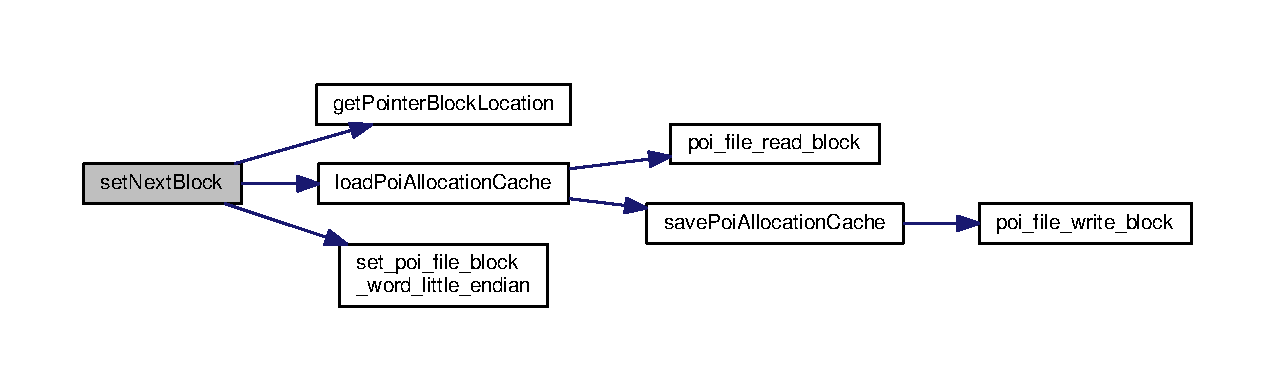
\includegraphics[width=350pt]{allocation-block-manager_8c_a7387272862663d2af1af9d5c21cddc84_cgraph}
\end{center}
\end{figure}




Here is the caller graph for this function\-:\nopagebreak
\begin{figure}[H]
\begin{center}
\leavevmode
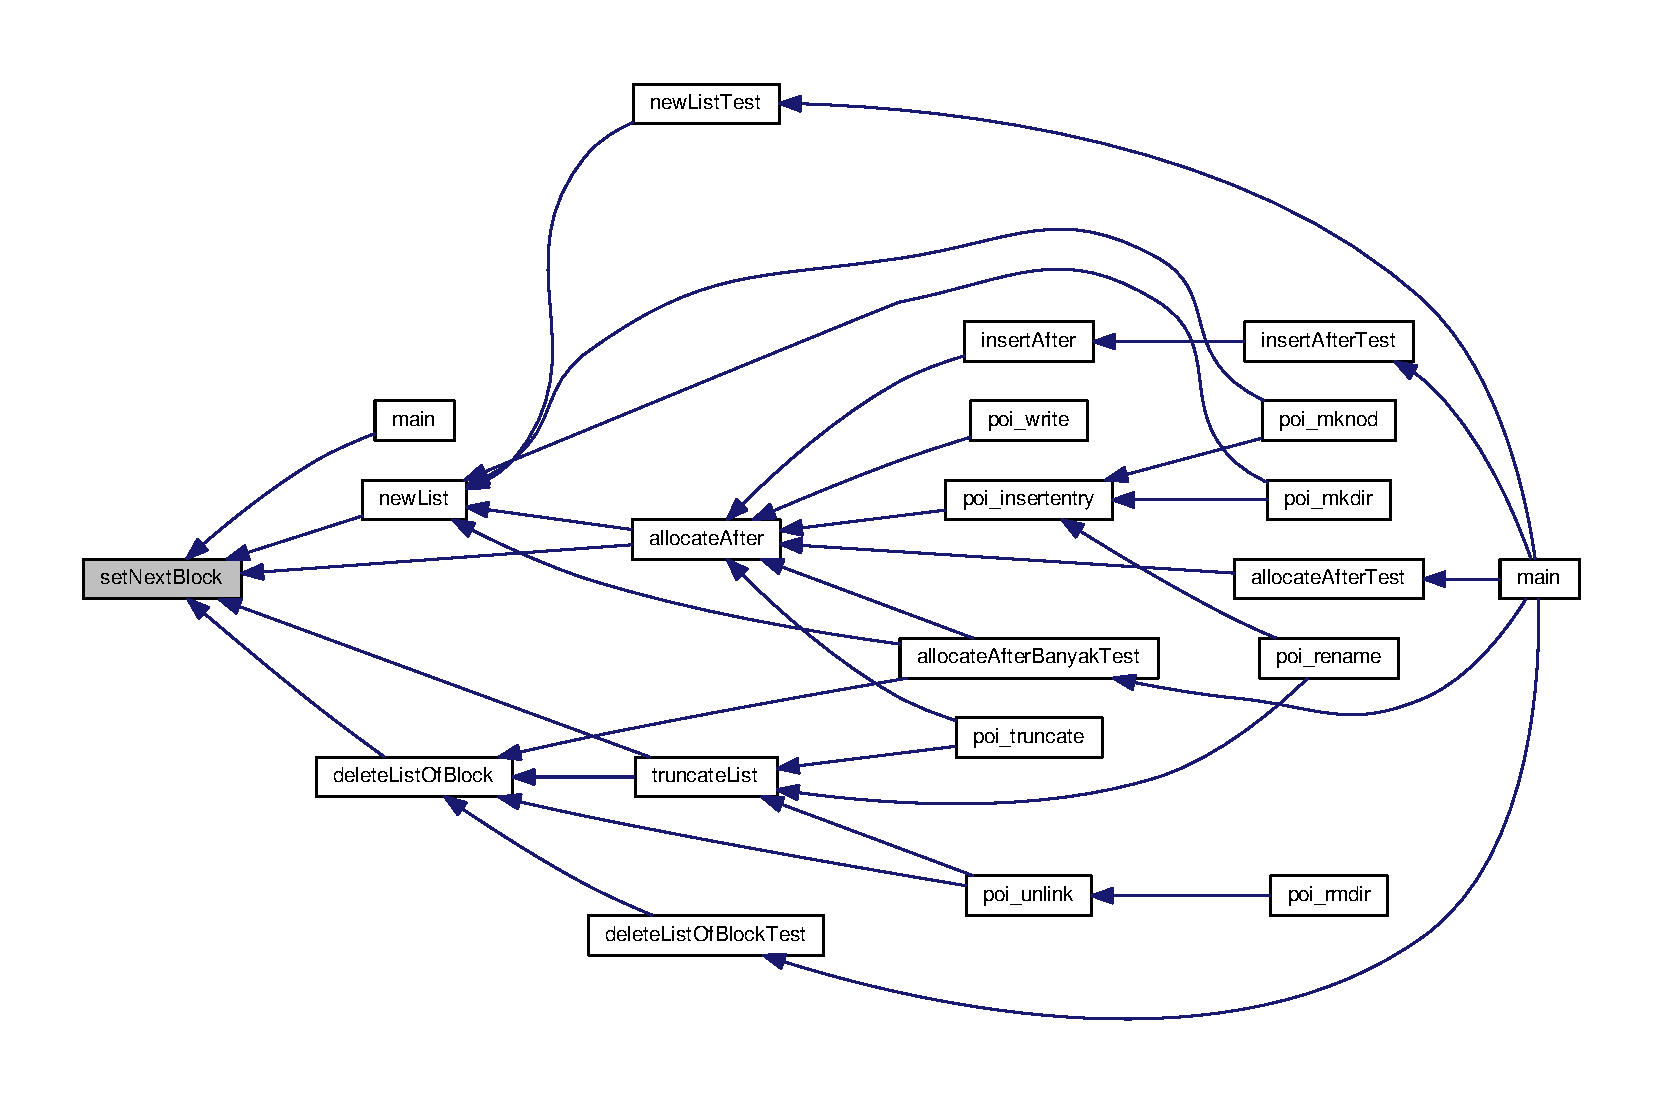
\includegraphics[width=350pt]{allocation-block-manager_8c_a7387272862663d2af1af9d5c21cddc84_icgraph}
\end{center}
\end{figure}




\subsection{Variable Documentation}
\hypertarget{allocation-block-manager_8c_a8cca9731003c6880e9aa8c3eb9d24951}{\index{allocation-\/block-\/manager.\-c@{allocation-\/block-\/manager.\-c}!poi\-\_\-allocation\-\_\-cache@{poi\-\_\-allocation\-\_\-cache}}
\index{poi\-\_\-allocation\-\_\-cache@{poi\-\_\-allocation\-\_\-cache}!allocation-block-manager.c@{allocation-\/block-\/manager.\-c}}
\subsubsection[{poi\-\_\-allocation\-\_\-cache}]{\setlength{\rightskip}{0pt plus 5cm}{\bf poi\-\_\-file\-\_\-block} poi\-\_\-allocation\-\_\-cache}}\label{allocation-block-manager_8c_a8cca9731003c6880e9aa8c3eb9d24951}
\hypertarget{allocation-block-manager_8c_a0f8b81672add5e3cee6cadcec0ff91b6}{\index{allocation-\/block-\/manager.\-c@{allocation-\/block-\/manager.\-c}!poi\-\_\-allocation\-\_\-cache\-\_\-file\-\_\-block\-\_\-num@{poi\-\_\-allocation\-\_\-cache\-\_\-file\-\_\-block\-\_\-num}}
\index{poi\-\_\-allocation\-\_\-cache\-\_\-file\-\_\-block\-\_\-num@{poi\-\_\-allocation\-\_\-cache\-\_\-file\-\_\-block\-\_\-num}!allocation-block-manager.c@{allocation-\/block-\/manager.\-c}}
\subsubsection[{poi\-\_\-allocation\-\_\-cache\-\_\-file\-\_\-block\-\_\-num}]{\setlength{\rightskip}{0pt plus 5cm}int poi\-\_\-allocation\-\_\-cache\-\_\-file\-\_\-block\-\_\-num = 0}}\label{allocation-block-manager_8c_a0f8b81672add5e3cee6cadcec0ff91b6}

\hypertarget{allocation-block-manager_8h}{\section{src/allocation-\/block-\/manager.h File Reference}
\label{allocation-block-manager_8h}\index{src/allocation-\/block-\/manager.\-h@{src/allocation-\/block-\/manager.\-h}}
}
{\ttfamily \#include \char`\"{}file-\/manager.\-h\char`\"{}}\\*
{\ttfamily \#include \char`\"{}data-\/pool-\/block-\/manager.\-h\char`\"{}}\\*
{\ttfamily \#include $<$stdbool.\-h$>$}\\*
Include dependency graph for allocation-\/block-\/manager.h\-:
\nopagebreak
\begin{figure}[H]
\begin{center}
\leavevmode
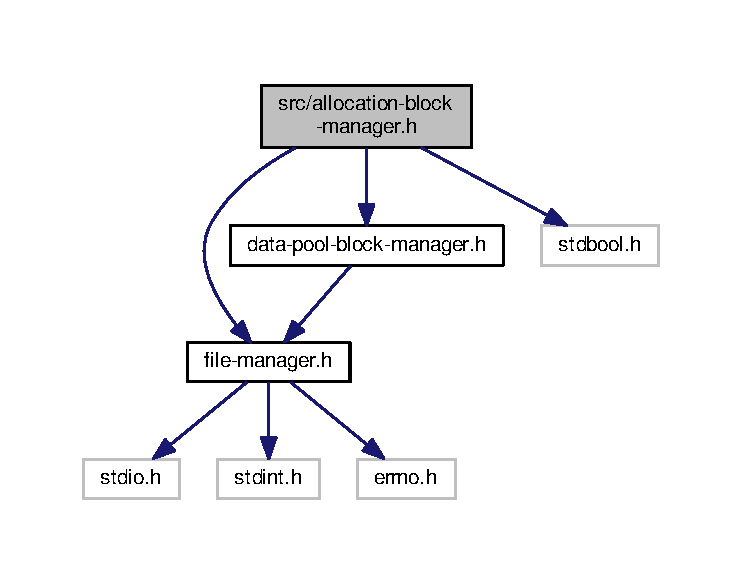
\includegraphics[width=350pt]{allocation-block-manager_8h__incl}
\end{center}
\end{figure}
This graph shows which files directly or indirectly include this file\-:
\nopagebreak
\begin{figure}[H]
\begin{center}
\leavevmode
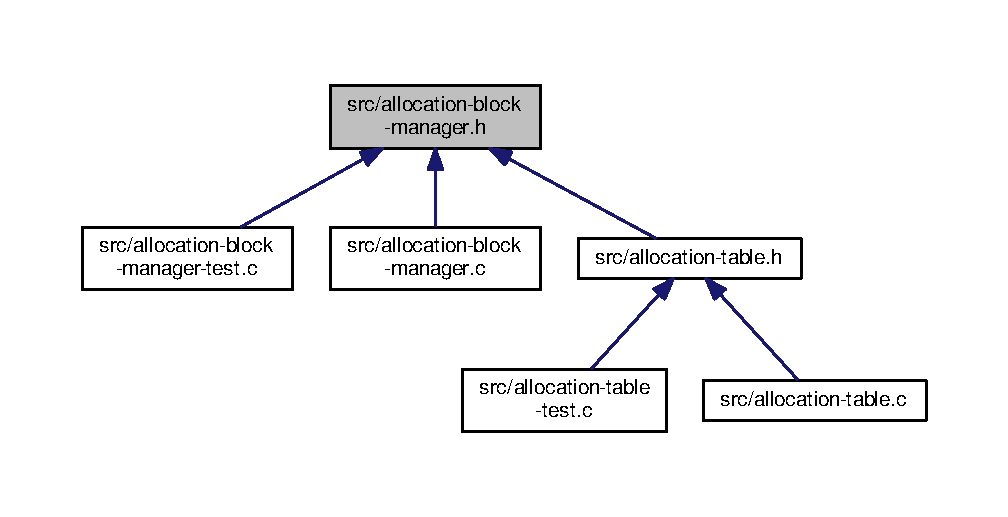
\includegraphics[width=350pt]{allocation-block-manager_8h__dep__incl}
\end{center}
\end{figure}
\subsection*{Functions}
\begin{DoxyCompactItemize}
\item 
void \hyperlink{allocation-block-manager_8h_a2d77f886ffa0a0d025a6a521cc6cf294}{load\-Poi\-Allocation\-Cache} (\hyperlink{file-manager_8h_aef709af8fc6566dcaf55b656bb9f8881}{poi\-\_\-file\-\_\-block\-\_\-num\-\_\-t} \hyperlink{allocation-table-test_8c_a24010dade8ebab3f87a48022772cd975}{n})
\item 
void \hyperlink{allocation-block-manager_8h_aa62c7923af0be489b52b1dcdd7c04e23}{save\-Poi\-Allocation\-Cache} ()
\item 
bool \hyperlink{allocation-block-manager_8h_a4b553c2a61827a60738c9323e6082903}{is\-Empty} (\hyperlink{data-pool-block-manager_8h_a87e19ab8290bcd76be1c7db1e90cc6f6}{poi\-\_\-data\-\_\-pool\-\_\-block\-\_\-idx\-\_\-t} \hyperlink{allocation-table-test_8c_a24010dade8ebab3f87a48022772cd975}{n})
\item 
\hyperlink{data-pool-block-manager_8h_a87e19ab8290bcd76be1c7db1e90cc6f6}{poi\-\_\-data\-\_\-pool\-\_\-block\-\_\-idx\-\_\-t} \hyperlink{allocation-block-manager_8h_a0843a74a7e1cc7c50dbfa521e4ea1cc8}{get\-Next\-Block} (\hyperlink{data-pool-block-manager_8h_a87e19ab8290bcd76be1c7db1e90cc6f6}{poi\-\_\-data\-\_\-pool\-\_\-block\-\_\-idx\-\_\-t} \hyperlink{allocation-table-test_8c_a24010dade8ebab3f87a48022772cd975}{n})
\item 
void \hyperlink{allocation-block-manager_8h_a7387272862663d2af1af9d5c21cddc84}{set\-Next\-Block} (\hyperlink{data-pool-block-manager_8h_a87e19ab8290bcd76be1c7db1e90cc6f6}{poi\-\_\-data\-\_\-pool\-\_\-block\-\_\-idx\-\_\-t} current, \hyperlink{data-pool-block-manager_8h_a87e19ab8290bcd76be1c7db1e90cc6f6}{poi\-\_\-data\-\_\-pool\-\_\-block\-\_\-idx\-\_\-t} next)
\item 
\hyperlink{data-pool-block-manager_8h_a87e19ab8290bcd76be1c7db1e90cc6f6}{poi\-\_\-data\-\_\-pool\-\_\-block\-\_\-idx\-\_\-t} \hyperlink{allocation-block-manager_8h_ab352dc84382d70f0044e92c52165c2cc}{get\-Next\-Empty} (\hyperlink{data-pool-block-manager_8h_a87e19ab8290bcd76be1c7db1e90cc6f6}{poi\-\_\-data\-\_\-pool\-\_\-block\-\_\-idx\-\_\-t} \hyperlink{allocation-table-test_8c_a24010dade8ebab3f87a48022772cd975}{n})
\end{DoxyCompactItemize}


\subsection{Function Documentation}
\hypertarget{allocation-block-manager_8h_a0843a74a7e1cc7c50dbfa521e4ea1cc8}{\index{allocation-\/block-\/manager.\-h@{allocation-\/block-\/manager.\-h}!get\-Next\-Block@{get\-Next\-Block}}
\index{get\-Next\-Block@{get\-Next\-Block}!allocation-block-manager.h@{allocation-\/block-\/manager.\-h}}
\subsubsection[{get\-Next\-Block}]{\setlength{\rightskip}{0pt plus 5cm}{\bf poi\-\_\-data\-\_\-pool\-\_\-block\-\_\-idx\-\_\-t} get\-Next\-Block (
\begin{DoxyParamCaption}
\item[{{\bf poi\-\_\-data\-\_\-pool\-\_\-block\-\_\-idx\-\_\-t}}]{n}
\end{DoxyParamCaption}
)}}\label{allocation-block-manager_8h_a0843a74a7e1cc7c50dbfa521e4ea1cc8}


Definition at line 47 of file allocation-\/block-\/manager.\-c.



Here is the call graph for this function\-:
\nopagebreak
\begin{figure}[H]
\begin{center}
\leavevmode
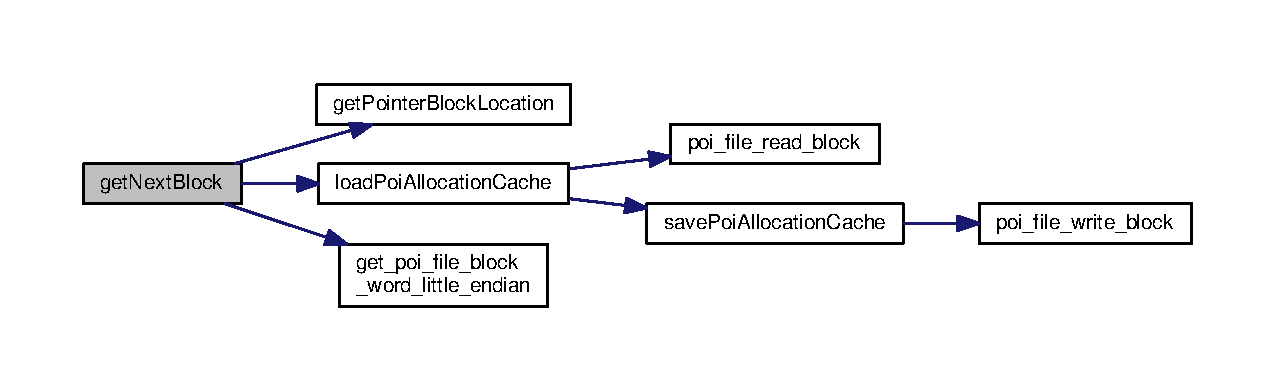
\includegraphics[width=350pt]{allocation-block-manager_8h_a0843a74a7e1cc7c50dbfa521e4ea1cc8_cgraph}
\end{center}
\end{figure}




Here is the caller graph for this function\-:
\nopagebreak
\begin{figure}[H]
\begin{center}
\leavevmode
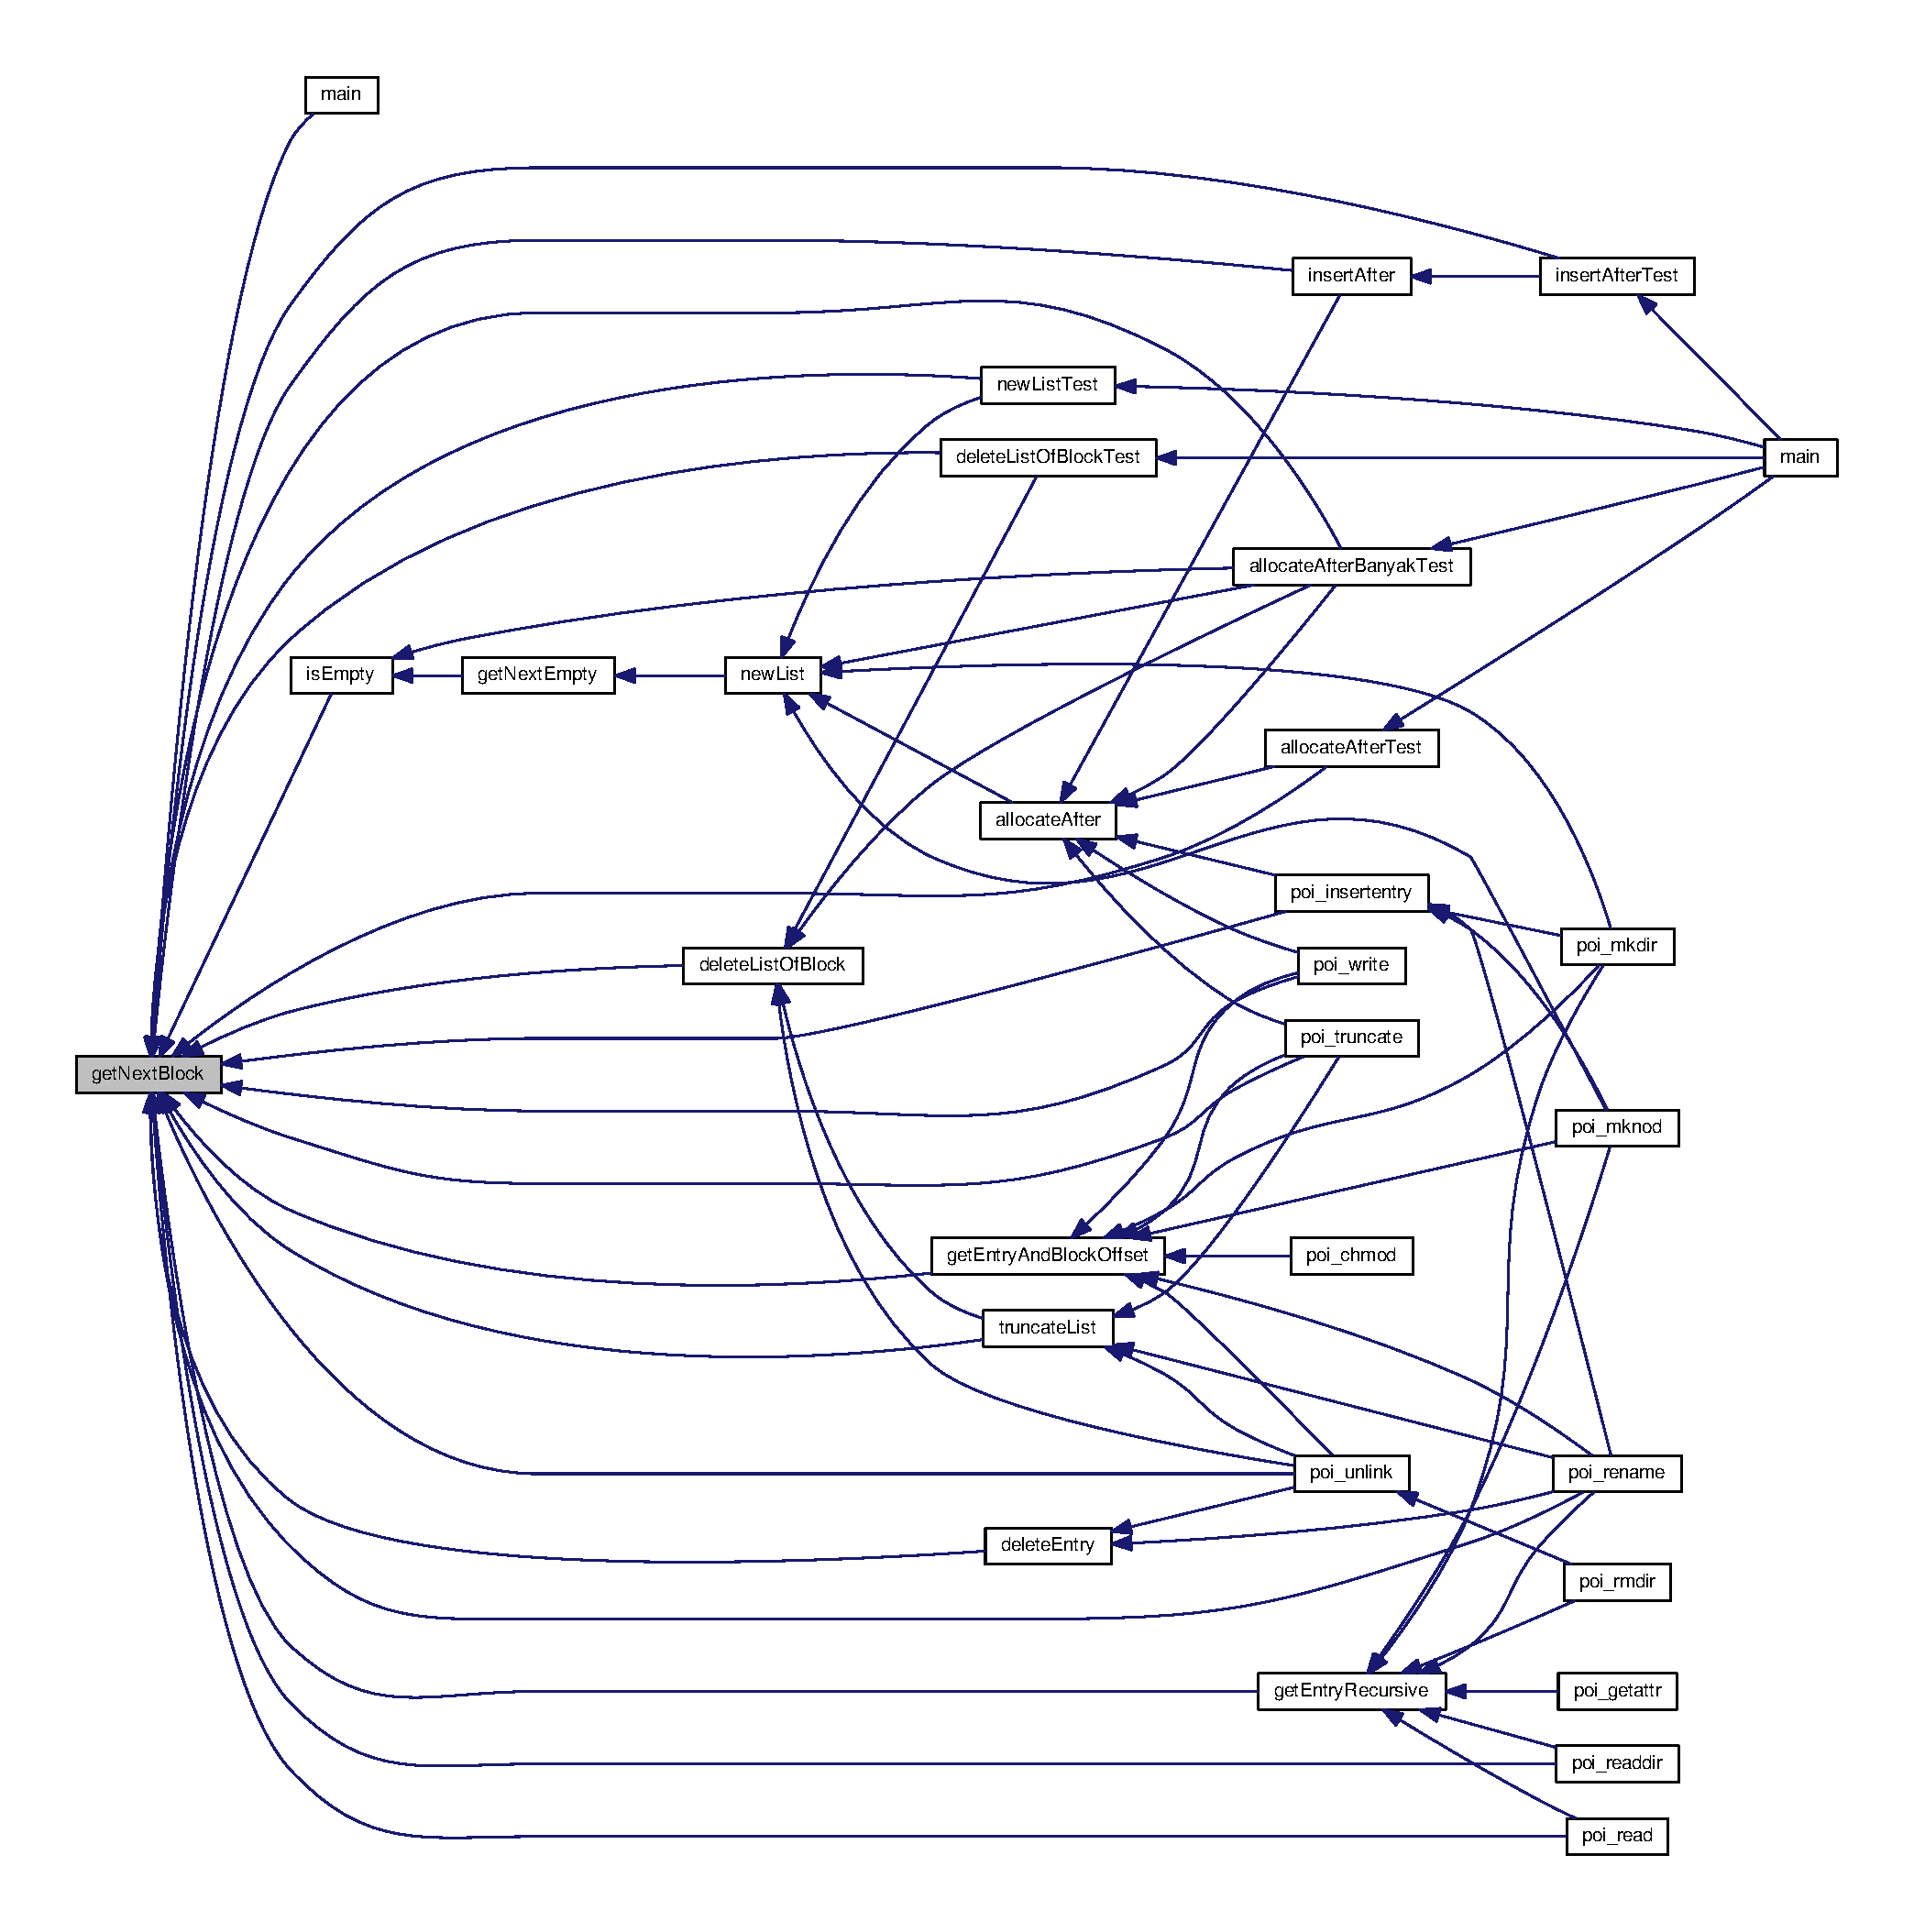
\includegraphics[width=350pt]{allocation-block-manager_8h_a0843a74a7e1cc7c50dbfa521e4ea1cc8_icgraph}
\end{center}
\end{figure}


\hypertarget{allocation-block-manager_8h_ab352dc84382d70f0044e92c52165c2cc}{\index{allocation-\/block-\/manager.\-h@{allocation-\/block-\/manager.\-h}!get\-Next\-Empty@{get\-Next\-Empty}}
\index{get\-Next\-Empty@{get\-Next\-Empty}!allocation-block-manager.h@{allocation-\/block-\/manager.\-h}}
\subsubsection[{get\-Next\-Empty}]{\setlength{\rightskip}{0pt plus 5cm}{\bf poi\-\_\-data\-\_\-pool\-\_\-block\-\_\-idx\-\_\-t} get\-Next\-Empty (
\begin{DoxyParamCaption}
\item[{{\bf poi\-\_\-data\-\_\-pool\-\_\-block\-\_\-idx\-\_\-t}}]{n}
\end{DoxyParamCaption}
)}}\label{allocation-block-manager_8h_ab352dc84382d70f0044e92c52165c2cc}


Definition at line 74 of file allocation-\/block-\/manager.\-c.



Here is the call graph for this function\-:
\nopagebreak
\begin{figure}[H]
\begin{center}
\leavevmode
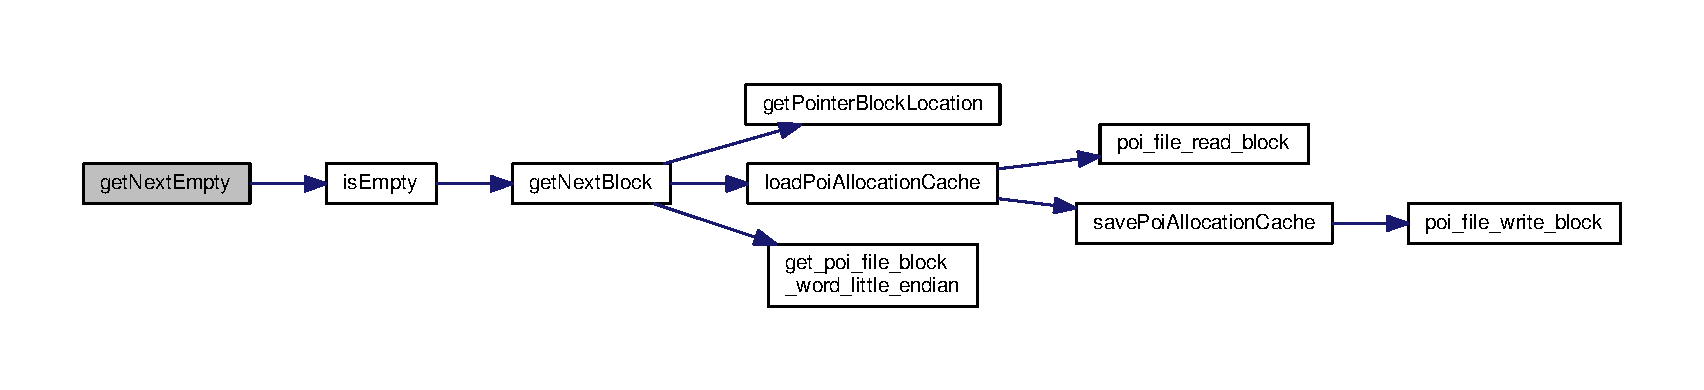
\includegraphics[width=350pt]{allocation-block-manager_8h_ab352dc84382d70f0044e92c52165c2cc_cgraph}
\end{center}
\end{figure}




Here is the caller graph for this function\-:
\nopagebreak
\begin{figure}[H]
\begin{center}
\leavevmode
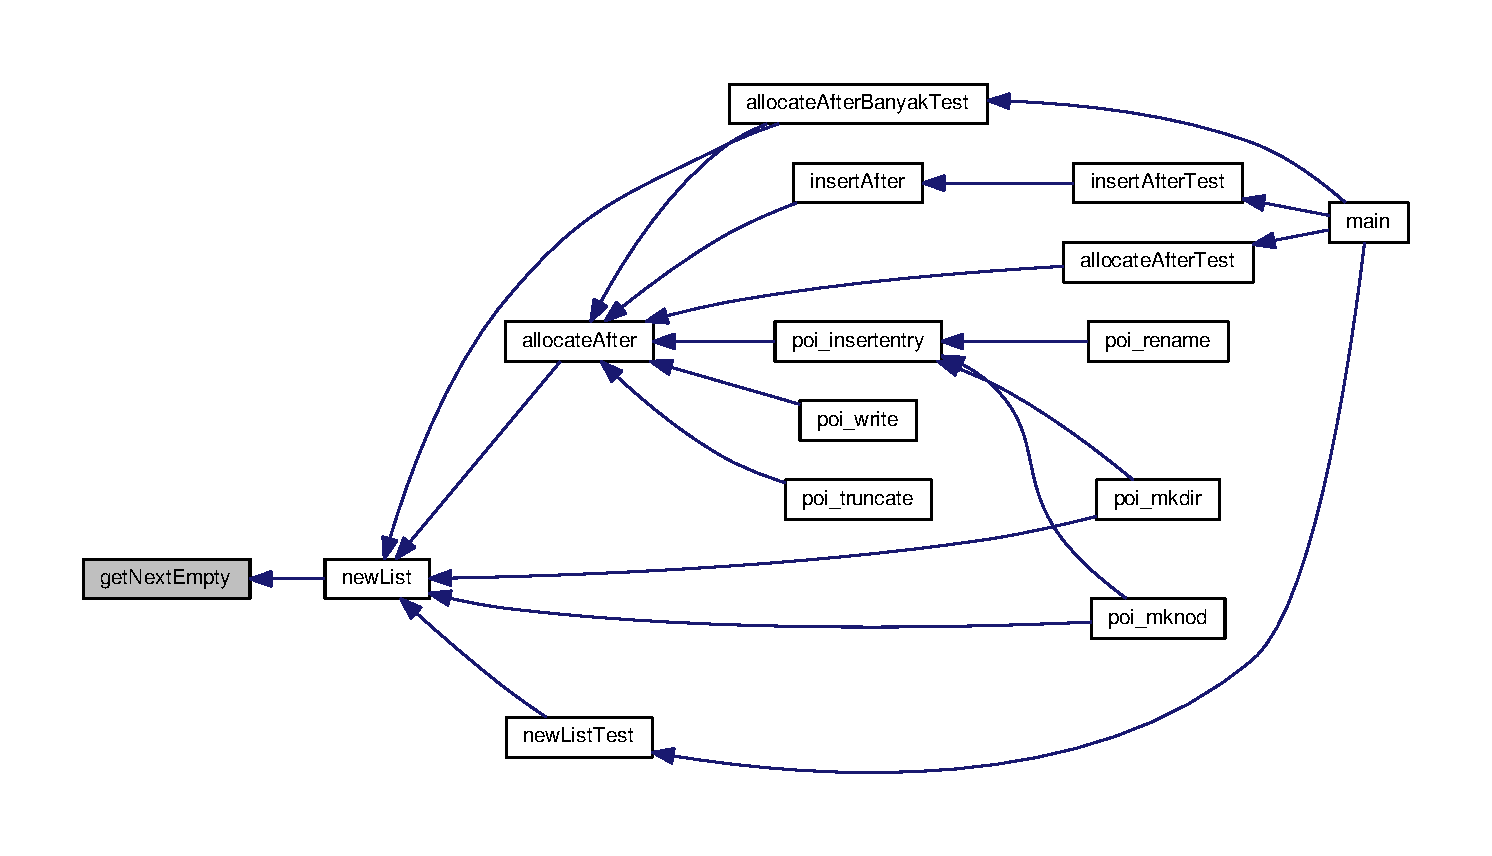
\includegraphics[width=350pt]{allocation-block-manager_8h_ab352dc84382d70f0044e92c52165c2cc_icgraph}
\end{center}
\end{figure}


\hypertarget{allocation-block-manager_8h_a4b553c2a61827a60738c9323e6082903}{\index{allocation-\/block-\/manager.\-h@{allocation-\/block-\/manager.\-h}!is\-Empty@{is\-Empty}}
\index{is\-Empty@{is\-Empty}!allocation-block-manager.h@{allocation-\/block-\/manager.\-h}}
\subsubsection[{is\-Empty}]{\setlength{\rightskip}{0pt plus 5cm}bool is\-Empty (
\begin{DoxyParamCaption}
\item[{{\bf poi\-\_\-data\-\_\-pool\-\_\-block\-\_\-idx\-\_\-t}}]{n}
\end{DoxyParamCaption}
)}}\label{allocation-block-manager_8h_a4b553c2a61827a60738c9323e6082903}


Definition at line 34 of file allocation-\/block-\/manager.\-c.



Here is the call graph for this function\-:
\nopagebreak
\begin{figure}[H]
\begin{center}
\leavevmode
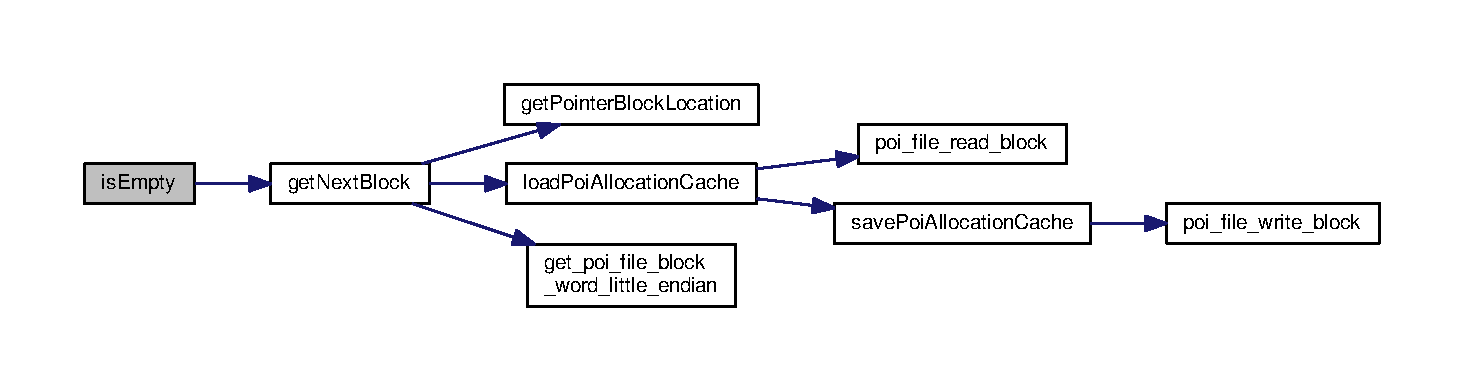
\includegraphics[width=350pt]{allocation-block-manager_8h_a4b553c2a61827a60738c9323e6082903_cgraph}
\end{center}
\end{figure}




Here is the caller graph for this function\-:
\nopagebreak
\begin{figure}[H]
\begin{center}
\leavevmode
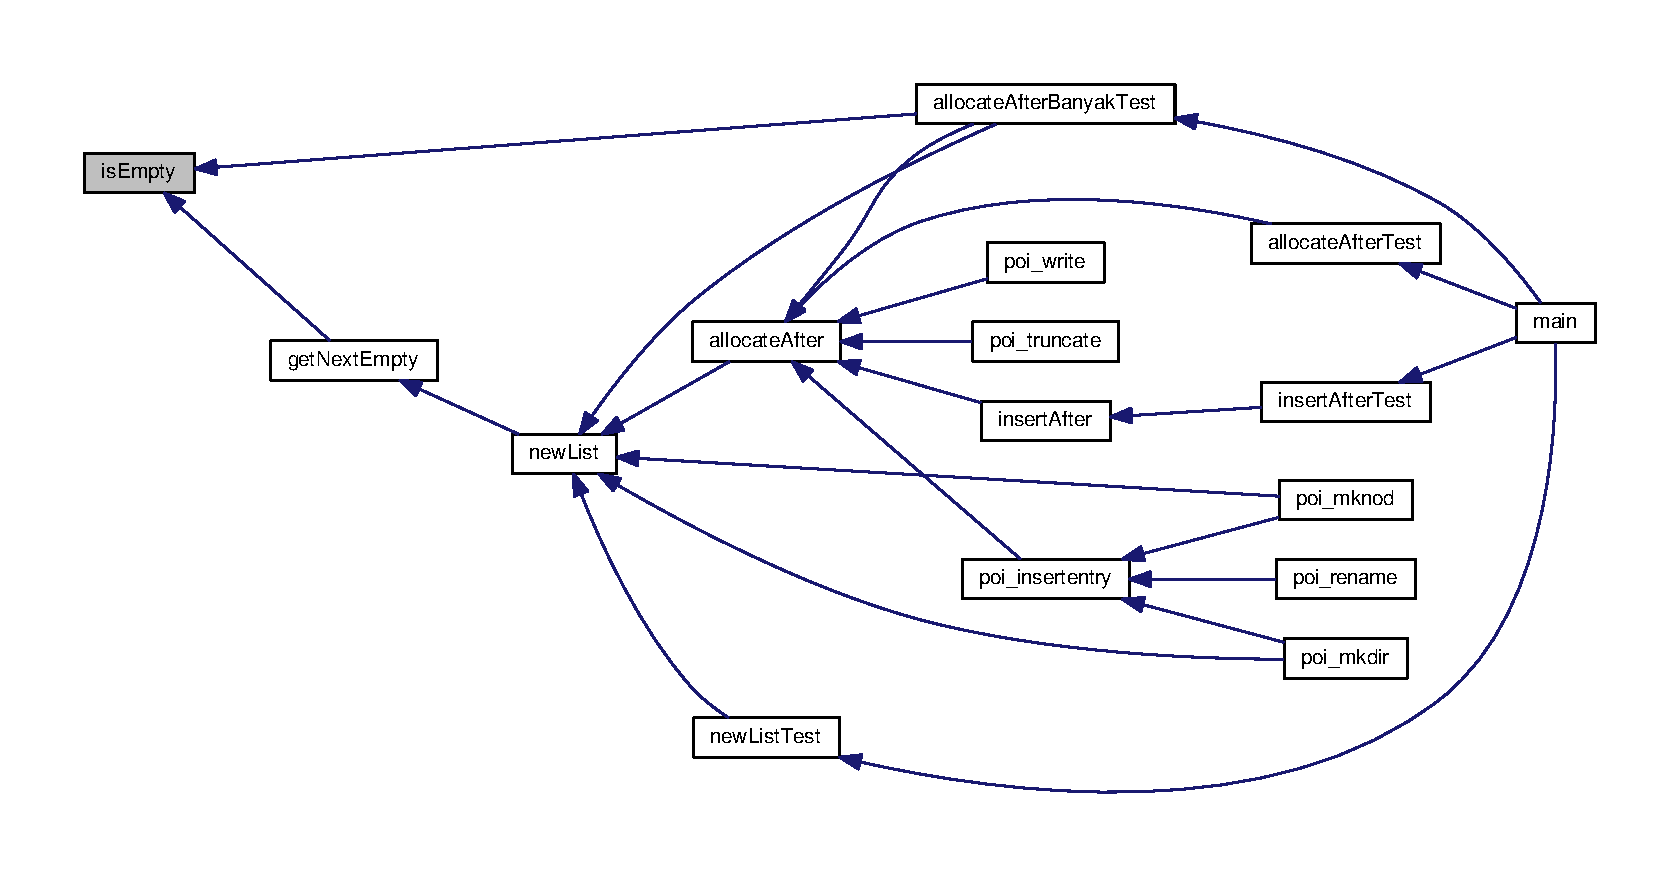
\includegraphics[width=350pt]{allocation-block-manager_8h_a4b553c2a61827a60738c9323e6082903_icgraph}
\end{center}
\end{figure}


\hypertarget{allocation-block-manager_8h_a2d77f886ffa0a0d025a6a521cc6cf294}{\index{allocation-\/block-\/manager.\-h@{allocation-\/block-\/manager.\-h}!load\-Poi\-Allocation\-Cache@{load\-Poi\-Allocation\-Cache}}
\index{load\-Poi\-Allocation\-Cache@{load\-Poi\-Allocation\-Cache}!allocation-block-manager.h@{allocation-\/block-\/manager.\-h}}
\subsubsection[{load\-Poi\-Allocation\-Cache}]{\setlength{\rightskip}{0pt plus 5cm}void load\-Poi\-Allocation\-Cache (
\begin{DoxyParamCaption}
\item[{{\bf poi\-\_\-file\-\_\-block\-\_\-num\-\_\-t}}]{n}
\end{DoxyParamCaption}
)}}\label{allocation-block-manager_8h_a2d77f886ffa0a0d025a6a521cc6cf294}


Definition at line 12 of file allocation-\/block-\/manager.\-c.



Here is the call graph for this function\-:
\nopagebreak
\begin{figure}[H]
\begin{center}
\leavevmode
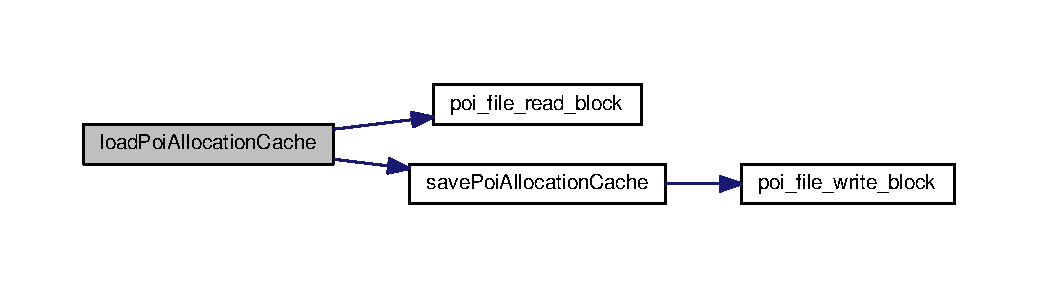
\includegraphics[width=350pt]{allocation-block-manager_8h_a2d77f886ffa0a0d025a6a521cc6cf294_cgraph}
\end{center}
\end{figure}




Here is the caller graph for this function\-:
\nopagebreak
\begin{figure}[H]
\begin{center}
\leavevmode
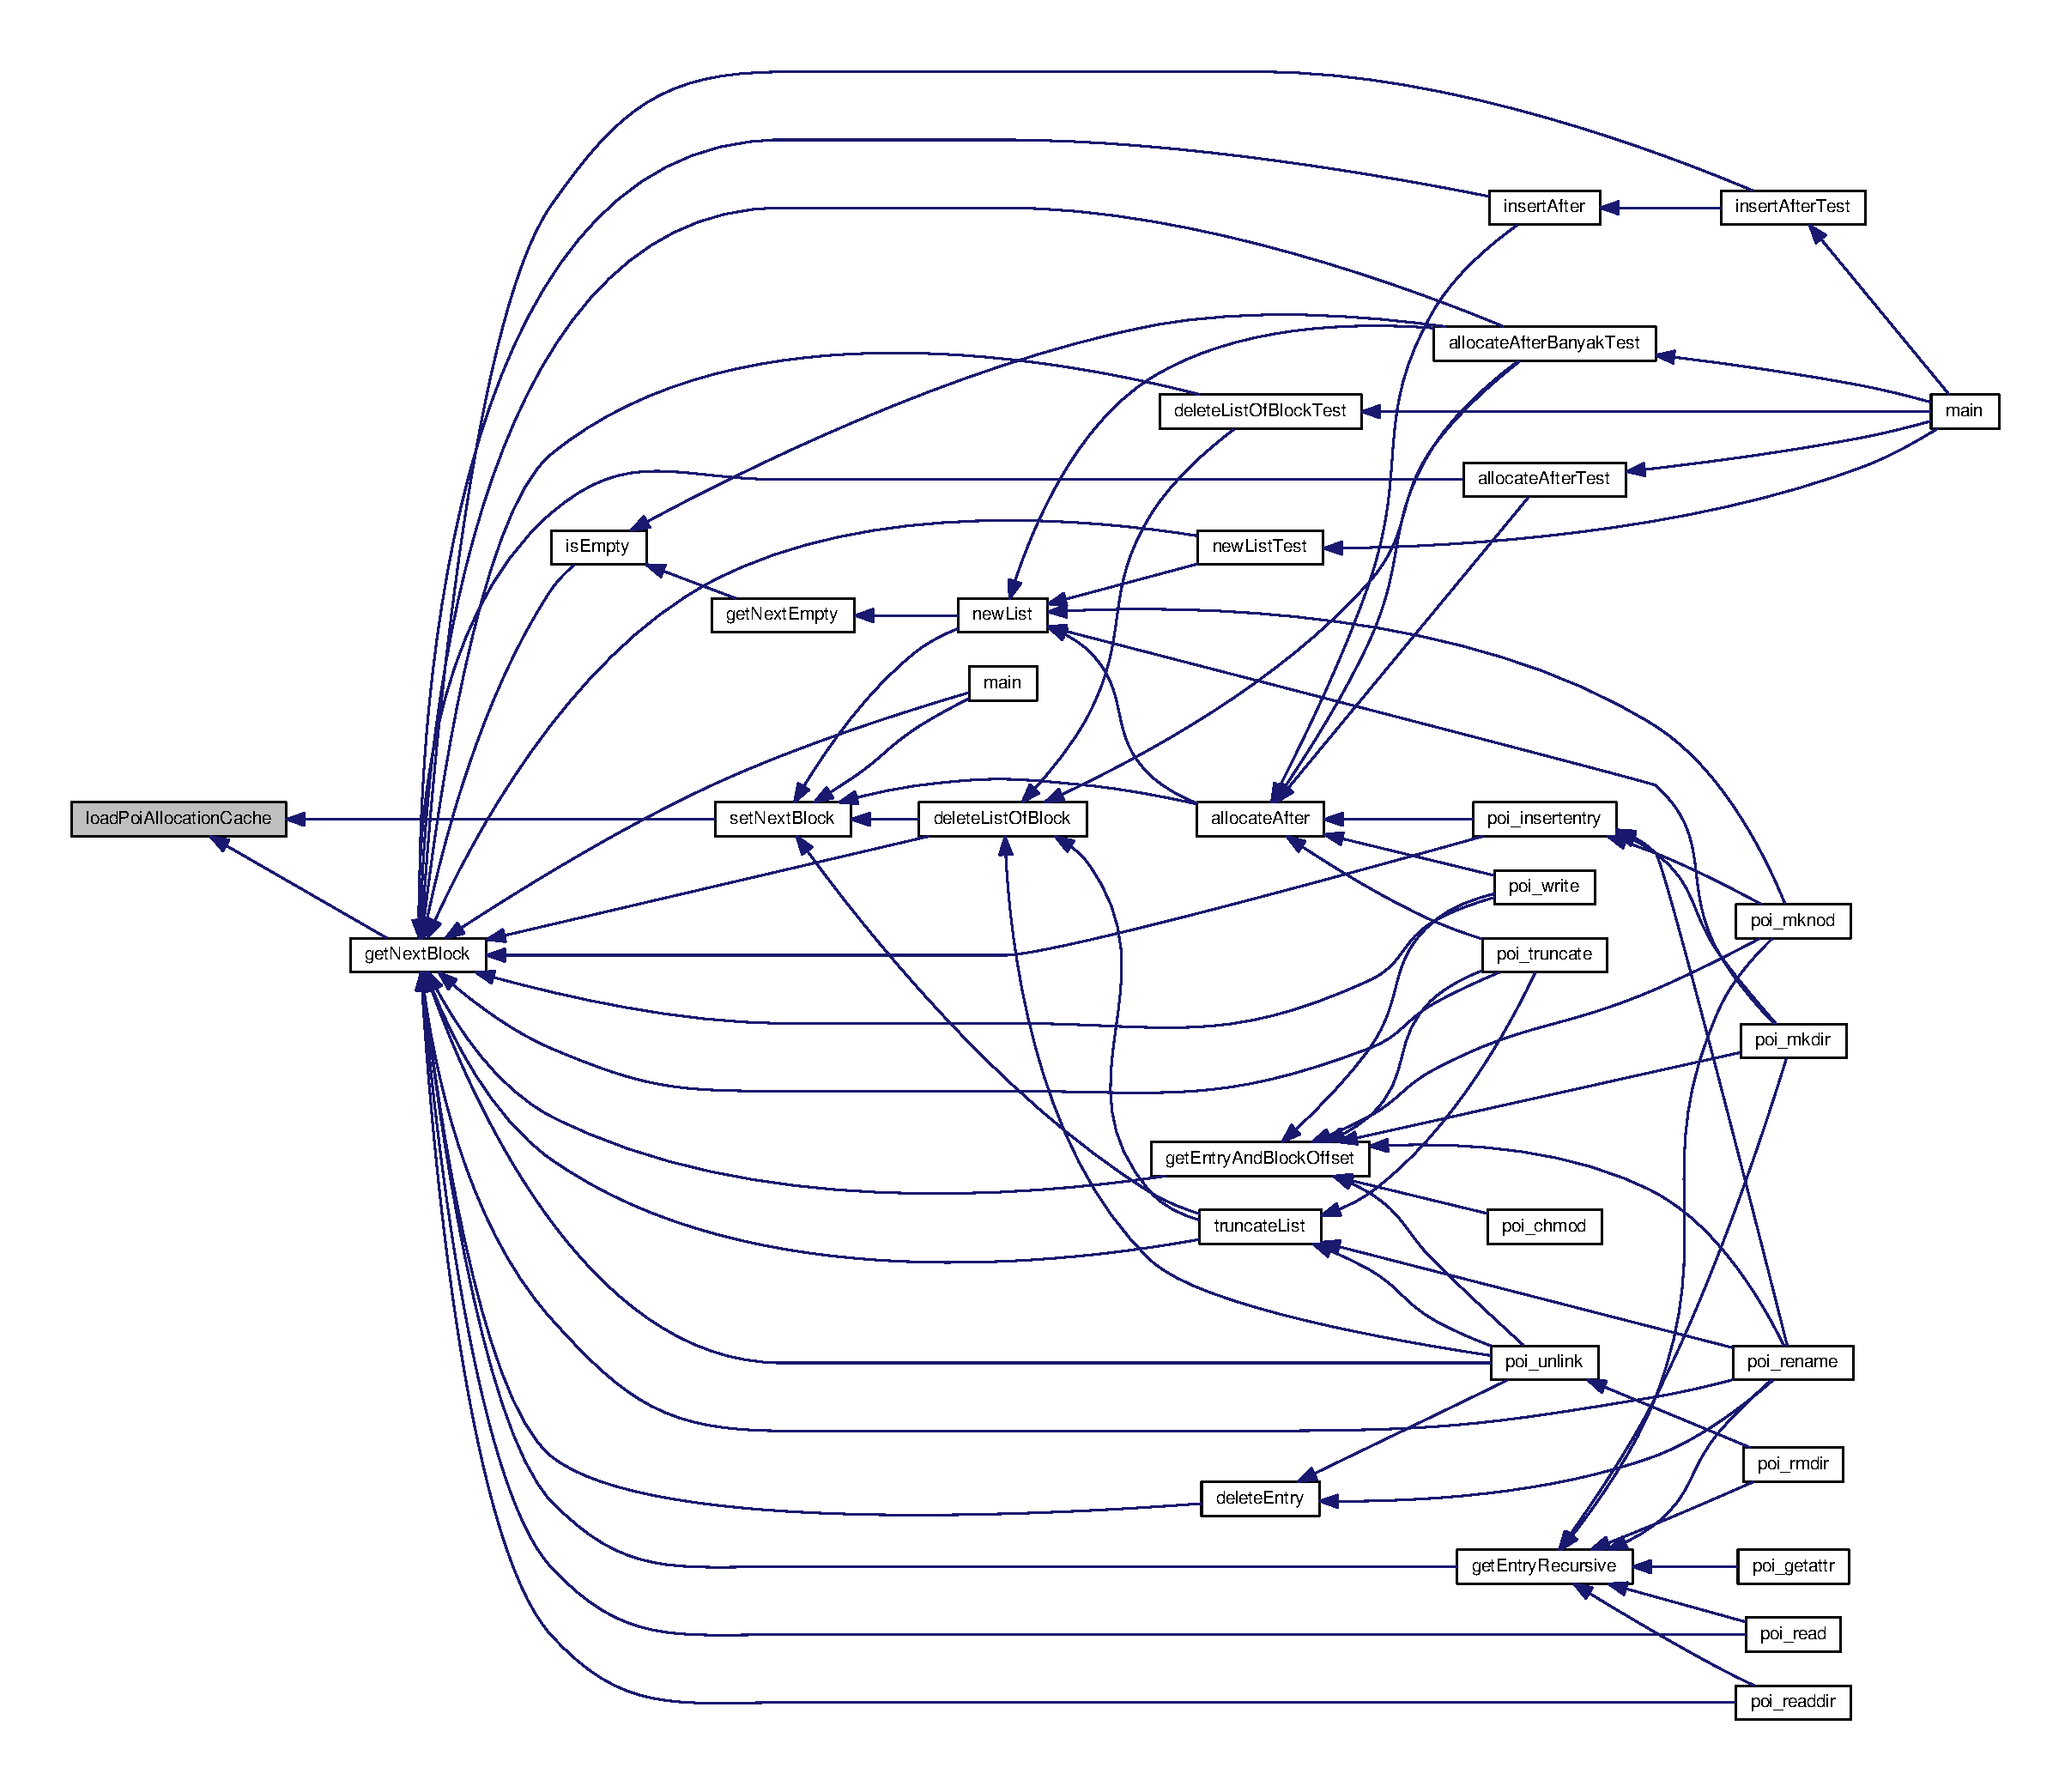
\includegraphics[width=350pt]{allocation-block-manager_8h_a2d77f886ffa0a0d025a6a521cc6cf294_icgraph}
\end{center}
\end{figure}


\hypertarget{allocation-block-manager_8h_aa62c7923af0be489b52b1dcdd7c04e23}{\index{allocation-\/block-\/manager.\-h@{allocation-\/block-\/manager.\-h}!save\-Poi\-Allocation\-Cache@{save\-Poi\-Allocation\-Cache}}
\index{save\-Poi\-Allocation\-Cache@{save\-Poi\-Allocation\-Cache}!allocation-block-manager.h@{allocation-\/block-\/manager.\-h}}
\subsubsection[{save\-Poi\-Allocation\-Cache}]{\setlength{\rightskip}{0pt plus 5cm}void save\-Poi\-Allocation\-Cache (
\begin{DoxyParamCaption}
{}
\end{DoxyParamCaption}
)}}\label{allocation-block-manager_8h_aa62c7923af0be489b52b1dcdd7c04e23}


Definition at line 25 of file allocation-\/block-\/manager.\-c.



Here is the call graph for this function\-:
\nopagebreak
\begin{figure}[H]
\begin{center}
\leavevmode
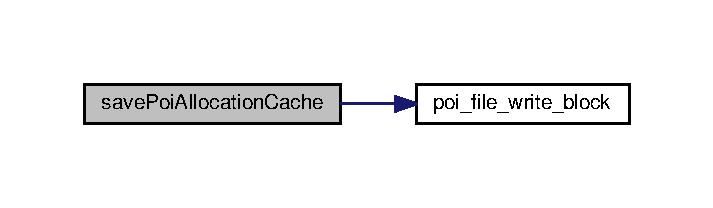
\includegraphics[width=342pt]{allocation-block-manager_8h_aa62c7923af0be489b52b1dcdd7c04e23_cgraph}
\end{center}
\end{figure}




Here is the caller graph for this function\-:
\nopagebreak
\begin{figure}[H]
\begin{center}
\leavevmode
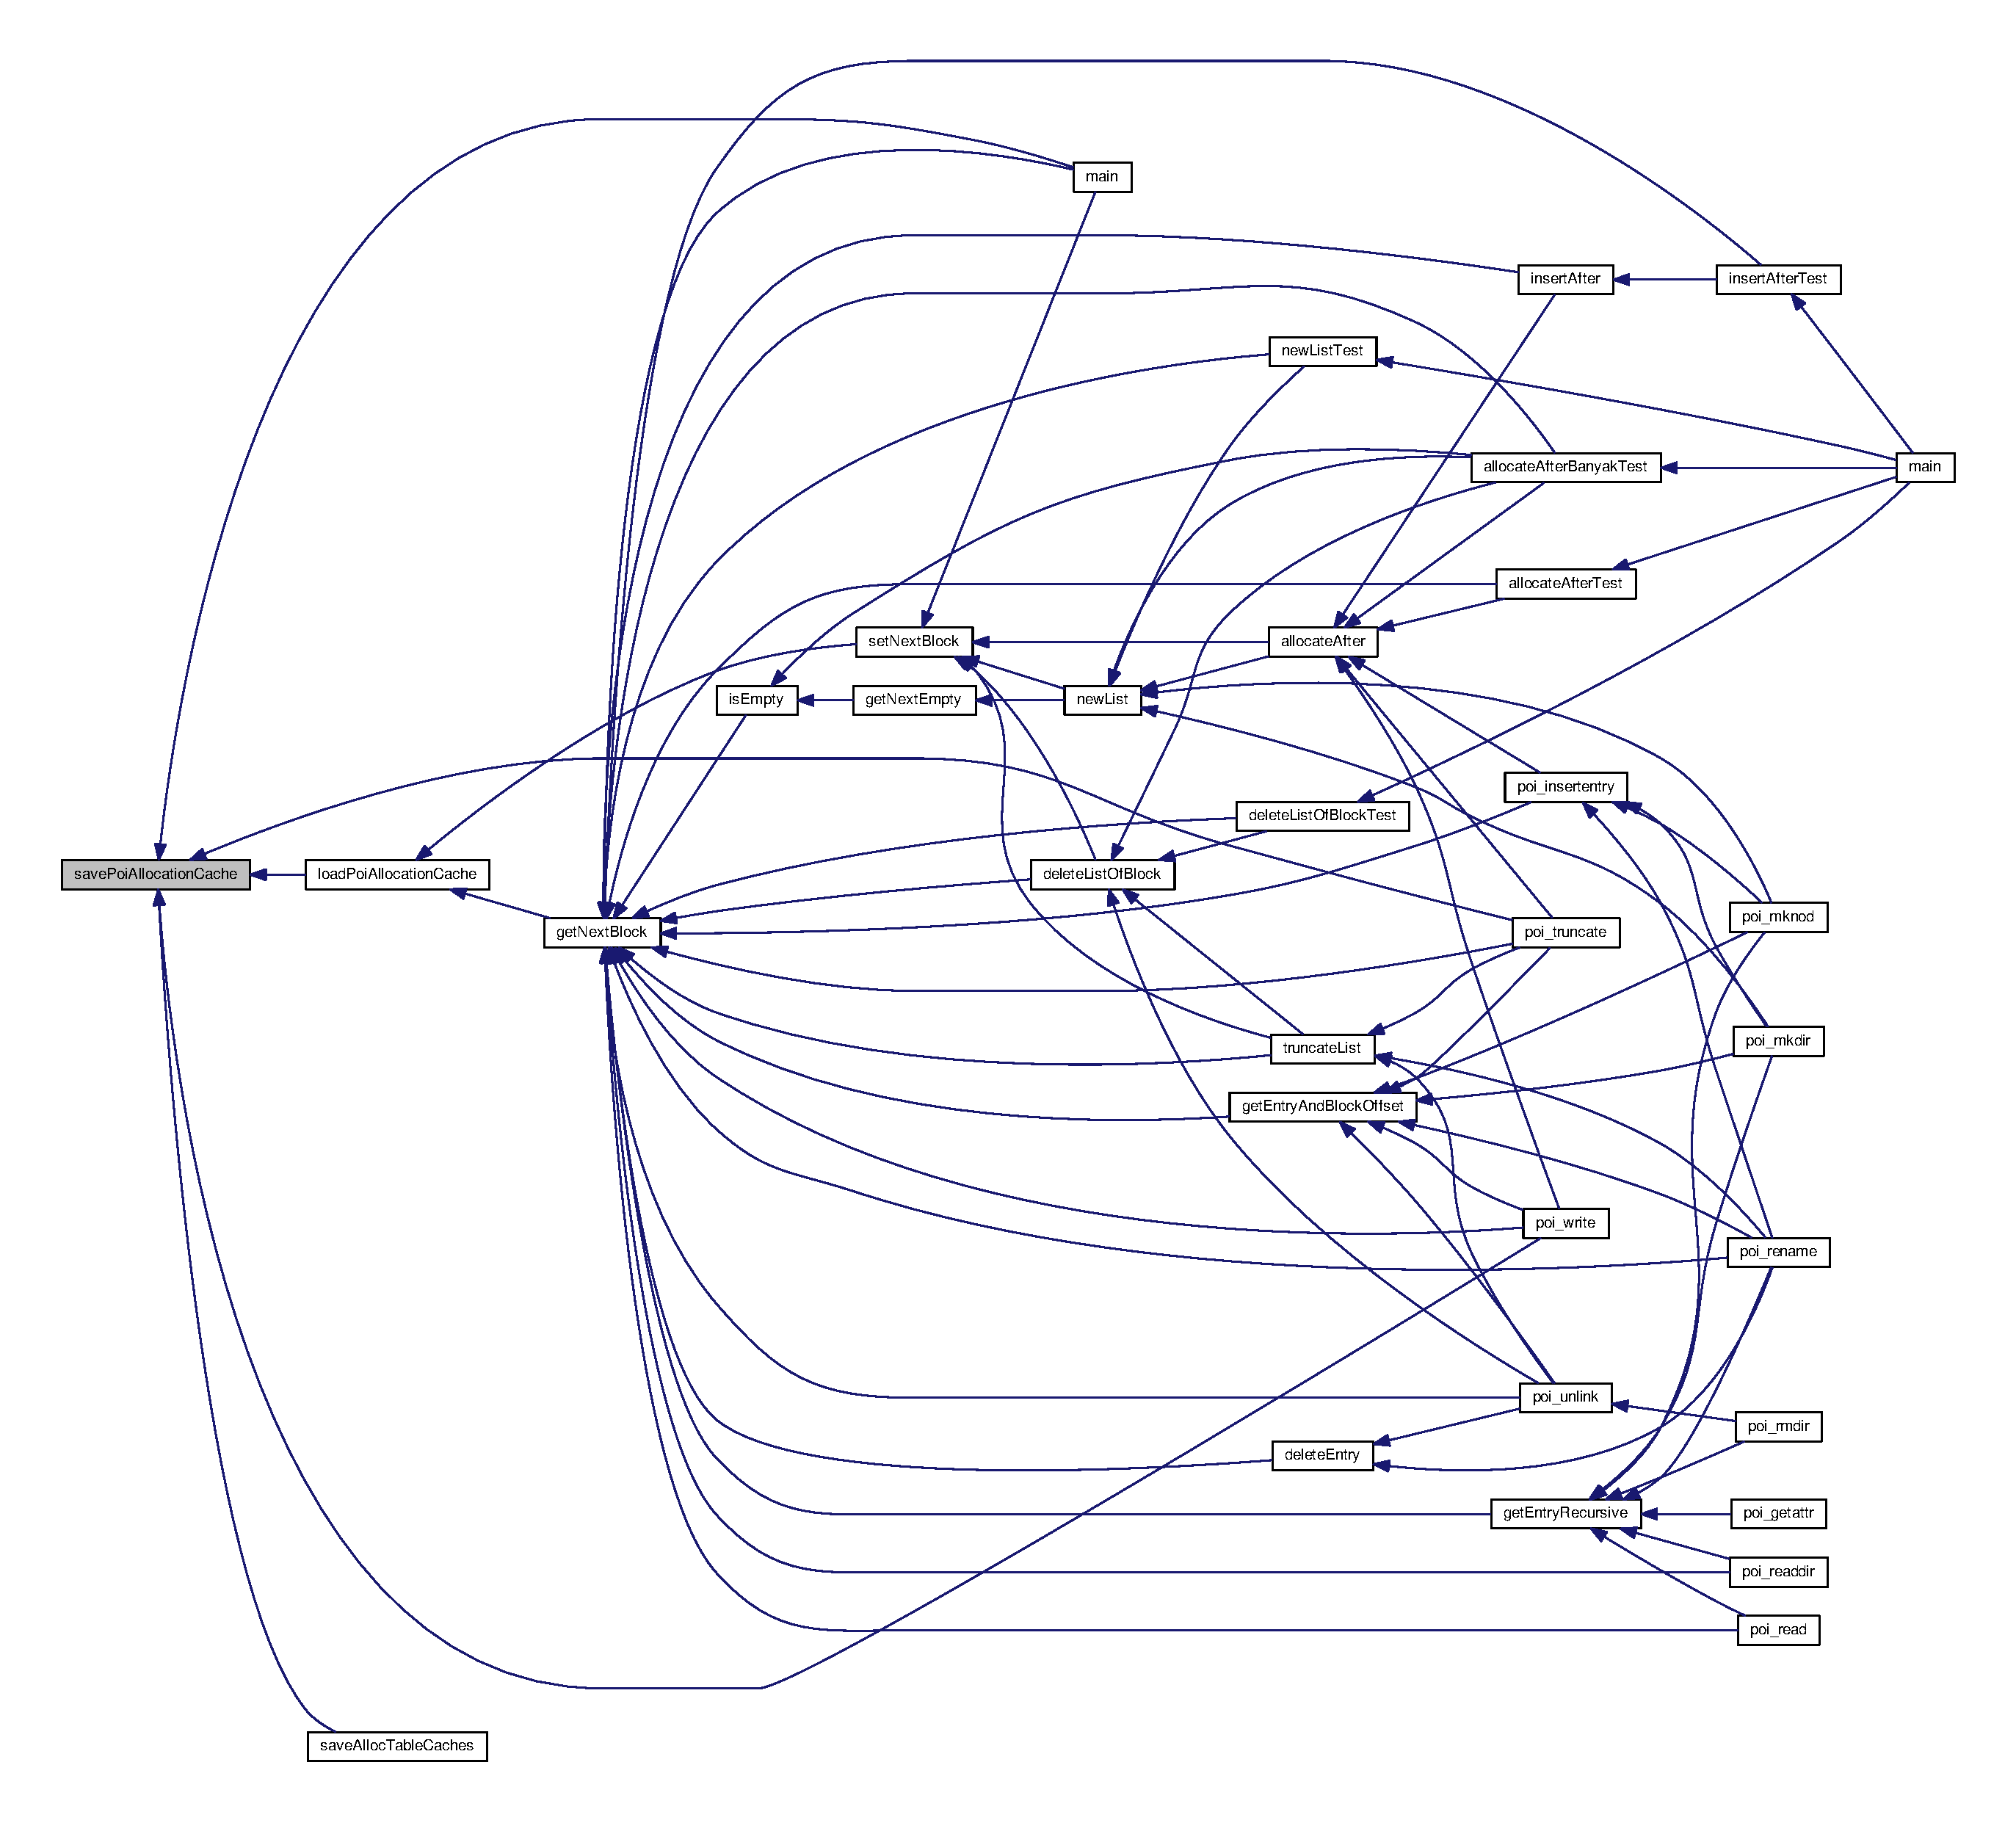
\includegraphics[width=350pt]{allocation-block-manager_8h_aa62c7923af0be489b52b1dcdd7c04e23_icgraph}
\end{center}
\end{figure}


\hypertarget{allocation-block-manager_8h_a7387272862663d2af1af9d5c21cddc84}{\index{allocation-\/block-\/manager.\-h@{allocation-\/block-\/manager.\-h}!set\-Next\-Block@{set\-Next\-Block}}
\index{set\-Next\-Block@{set\-Next\-Block}!allocation-block-manager.h@{allocation-\/block-\/manager.\-h}}
\subsubsection[{set\-Next\-Block}]{\setlength{\rightskip}{0pt plus 5cm}void set\-Next\-Block (
\begin{DoxyParamCaption}
\item[{{\bf poi\-\_\-data\-\_\-pool\-\_\-block\-\_\-idx\-\_\-t}}]{current, }
\item[{{\bf poi\-\_\-data\-\_\-pool\-\_\-block\-\_\-idx\-\_\-t}}]{next}
\end{DoxyParamCaption}
)}}\label{allocation-block-manager_8h_a7387272862663d2af1af9d5c21cddc84}


Definition at line 59 of file allocation-\/block-\/manager.\-c.



Here is the call graph for this function\-:
\nopagebreak
\begin{figure}[H]
\begin{center}
\leavevmode
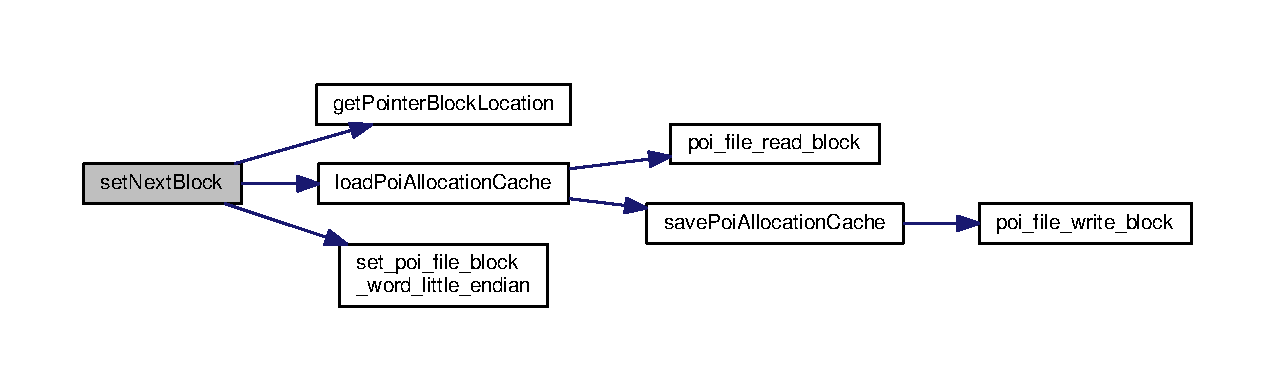
\includegraphics[width=350pt]{allocation-block-manager_8h_a7387272862663d2af1af9d5c21cddc84_cgraph}
\end{center}
\end{figure}




Here is the caller graph for this function\-:
\nopagebreak
\begin{figure}[H]
\begin{center}
\leavevmode
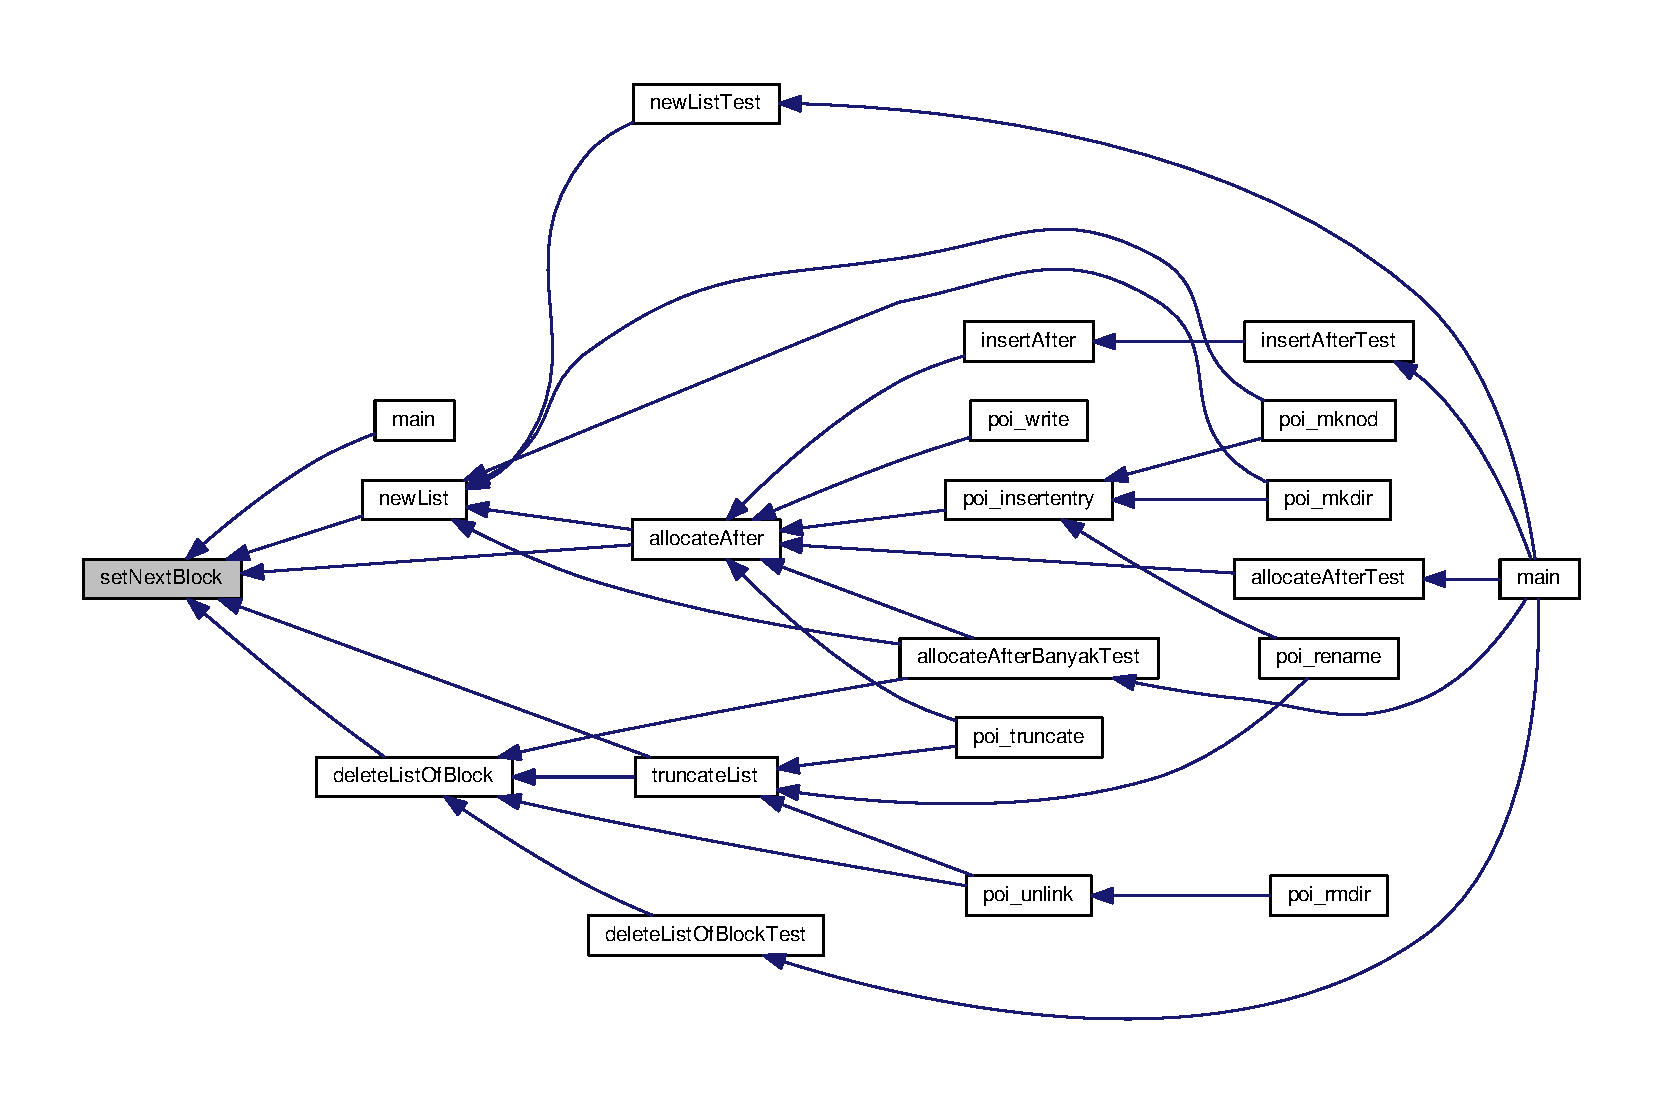
\includegraphics[width=350pt]{allocation-block-manager_8h_a7387272862663d2af1af9d5c21cddc84_icgraph}
\end{center}
\end{figure}



\hypertarget{allocation-manager_8h}{\section{src/allocation-\/manager.h File Reference}
\label{allocation-manager_8h}\index{src/allocation-\/manager.\-h@{src/allocation-\/manager.\-h}}
}


berkas sampah  


{\ttfamily \#include \char`\"{}file-\/manager.\-h\char`\"{}}\\*
{\ttfamily \#include \char`\"{}data-\/pool-\/block-\/manager.\-h\char`\"{}}\\*
{\ttfamily \#include $<$stdbool.\-h$>$}\\*
Include dependency graph for allocation-\/manager.h\-:\nopagebreak
\begin{figure}[H]
\begin{center}
\leavevmode
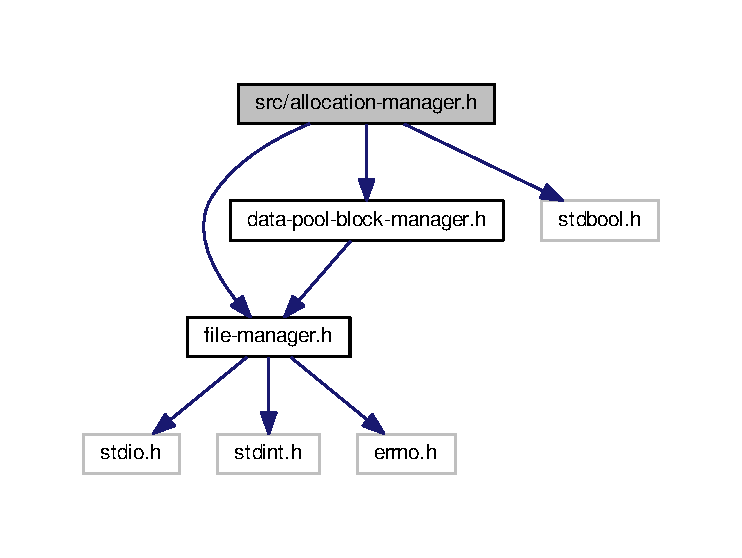
\includegraphics[width=350pt]{allocation-manager_8h__incl}
\end{center}
\end{figure}
\subsection*{Functions}
\begin{DoxyCompactItemize}
\item 
bool \hyperlink{allocation-manager_8h_a56b807a333a2fc6f627265865c1e9f7d}{is\-Empty} (poi\-\_\-data\-\_\-pool\-\_\-block\-\_\-num\-\_\-t \hyperlink{allocation-table-test_8c_a24010dade8ebab3f87a48022772cd975}{n})
\item 
poi\-\_\-data\-\_\-pool\-\_\-block\-\_\-num\-\_\-t \hyperlink{allocation-manager_8h_aac60c48ce4acad3a1d8e459ba5649259}{get\-Next\-Block} (poi\-\_\-data\-\_\-pool\-\_\-block\-\_\-num\-\_\-t \hyperlink{allocation-table-test_8c_a24010dade8ebab3f87a48022772cd975}{n})
\item 
poi\-\_\-data\-\_\-pool\-\_\-block\-\_\-num\-\_\-t \hyperlink{allocation-manager_8h_a98a30f2070bd2d0ace14f19f86484d16}{get\-Next\-Empty} (poi\-\_\-data\-\_\-pool\-\_\-block\-\_\-num\-\_\-t \hyperlink{allocation-table-test_8c_a24010dade8ebab3f87a48022772cd975}{n})
\end{DoxyCompactItemize}
\subsection*{Variables}
\begin{DoxyCompactItemize}
\item 
\hyperlink{structpoi__file__block}{poi\-\_\-file\-\_\-block} \hyperlink{allocation-manager_8h_a8cca9731003c6880e9aa8c3eb9d24951}{poi\-\_\-allocation\-\_\-cache}
\item 
int \hyperlink{allocation-manager_8h_a0f8b81672add5e3cee6cadcec0ff91b6}{poi\-\_\-allocation\-\_\-cache\-\_\-file\-\_\-block\-\_\-num}
\end{DoxyCompactItemize}


\subsection{Detailed Description}
berkas sampah \begin{DoxyAuthor}{Author}
jang berikoetnja 
\end{DoxyAuthor}


\subsection{Function Documentation}
\hypertarget{allocation-manager_8h_aac60c48ce4acad3a1d8e459ba5649259}{\index{allocation-\/manager.\-h@{allocation-\/manager.\-h}!get\-Next\-Block@{get\-Next\-Block}}
\index{get\-Next\-Block@{get\-Next\-Block}!allocation-manager.h@{allocation-\/manager.\-h}}
\subsubsection[{get\-Next\-Block}]{\setlength{\rightskip}{0pt plus 5cm}poi\-\_\-data\-\_\-pool\-\_\-block\-\_\-num\-\_\-t get\-Next\-Block (
\begin{DoxyParamCaption}
\item[{poi\-\_\-data\-\_\-pool\-\_\-block\-\_\-num\-\_\-t}]{n}
\end{DoxyParamCaption}
)}}\label{allocation-manager_8h_aac60c48ce4acad3a1d8e459ba5649259}
\hypertarget{allocation-manager_8h_a98a30f2070bd2d0ace14f19f86484d16}{\index{allocation-\/manager.\-h@{allocation-\/manager.\-h}!get\-Next\-Empty@{get\-Next\-Empty}}
\index{get\-Next\-Empty@{get\-Next\-Empty}!allocation-manager.h@{allocation-\/manager.\-h}}
\subsubsection[{get\-Next\-Empty}]{\setlength{\rightskip}{0pt plus 5cm}poi\-\_\-data\-\_\-pool\-\_\-block\-\_\-num\-\_\-t get\-Next\-Empty (
\begin{DoxyParamCaption}
\item[{poi\-\_\-data\-\_\-pool\-\_\-block\-\_\-num\-\_\-t}]{n}
\end{DoxyParamCaption}
)}}\label{allocation-manager_8h_a98a30f2070bd2d0ace14f19f86484d16}
\hypertarget{allocation-manager_8h_a56b807a333a2fc6f627265865c1e9f7d}{\index{allocation-\/manager.\-h@{allocation-\/manager.\-h}!is\-Empty@{is\-Empty}}
\index{is\-Empty@{is\-Empty}!allocation-manager.h@{allocation-\/manager.\-h}}
\subsubsection[{is\-Empty}]{\setlength{\rightskip}{0pt plus 5cm}bool is\-Empty (
\begin{DoxyParamCaption}
\item[{poi\-\_\-data\-\_\-pool\-\_\-block\-\_\-num\-\_\-t}]{n}
\end{DoxyParamCaption}
)}}\label{allocation-manager_8h_a56b807a333a2fc6f627265865c1e9f7d}


\subsection{Variable Documentation}
\hypertarget{allocation-manager_8h_a8cca9731003c6880e9aa8c3eb9d24951}{\index{allocation-\/manager.\-h@{allocation-\/manager.\-h}!poi\-\_\-allocation\-\_\-cache@{poi\-\_\-allocation\-\_\-cache}}
\index{poi\-\_\-allocation\-\_\-cache@{poi\-\_\-allocation\-\_\-cache}!allocation-manager.h@{allocation-\/manager.\-h}}
\subsubsection[{poi\-\_\-allocation\-\_\-cache}]{\setlength{\rightskip}{0pt plus 5cm}{\bf poi\-\_\-file\-\_\-block} poi\-\_\-allocation\-\_\-cache}}\label{allocation-manager_8h_a8cca9731003c6880e9aa8c3eb9d24951}
\hypertarget{allocation-manager_8h_a0f8b81672add5e3cee6cadcec0ff91b6}{\index{allocation-\/manager.\-h@{allocation-\/manager.\-h}!poi\-\_\-allocation\-\_\-cache\-\_\-file\-\_\-block\-\_\-num@{poi\-\_\-allocation\-\_\-cache\-\_\-file\-\_\-block\-\_\-num}}
\index{poi\-\_\-allocation\-\_\-cache\-\_\-file\-\_\-block\-\_\-num@{poi\-\_\-allocation\-\_\-cache\-\_\-file\-\_\-block\-\_\-num}!allocation-manager.h@{allocation-\/manager.\-h}}
\subsubsection[{poi\-\_\-allocation\-\_\-cache\-\_\-file\-\_\-block\-\_\-num}]{\setlength{\rightskip}{0pt plus 5cm}int poi\-\_\-allocation\-\_\-cache\-\_\-file\-\_\-block\-\_\-num}}\label{allocation-manager_8h_a0f8b81672add5e3cee6cadcec0ff91b6}

\hypertarget{allocation-table-test_8c}{\section{/home/nim\-\_\-13512501/\-Documents/tubes 2 O\-S/poi/src/allocation-\/table-\/test.c File Reference}
\label{allocation-table-test_8c}\index{/home/nim\-\_\-13512501/\-Documents/tubes 2 O\-S/poi/src/allocation-\/table-\/test.\-c@{/home/nim\-\_\-13512501/\-Documents/tubes 2 O\-S/poi/src/allocation-\/table-\/test.\-c}}
}


berkas penggerak uji untuk \hyperlink{allocation-table-test_8c}{allocation-\/table-\/test.\-c}  


{\ttfamily \#include \char`\"{}allocation-\/table.\-h\char`\"{}}\\*
{\ttfamily \#include $<$stdio.\-h$>$}\\*
{\ttfamily \#include $<$string.\-h$>$}\\*
{\ttfamily \#include $<$unistd.\-h$>$}\\*
Include dependency graph for allocation-\/table-\/test.c\-:\nopagebreak
\begin{figure}[H]
\begin{center}
\leavevmode
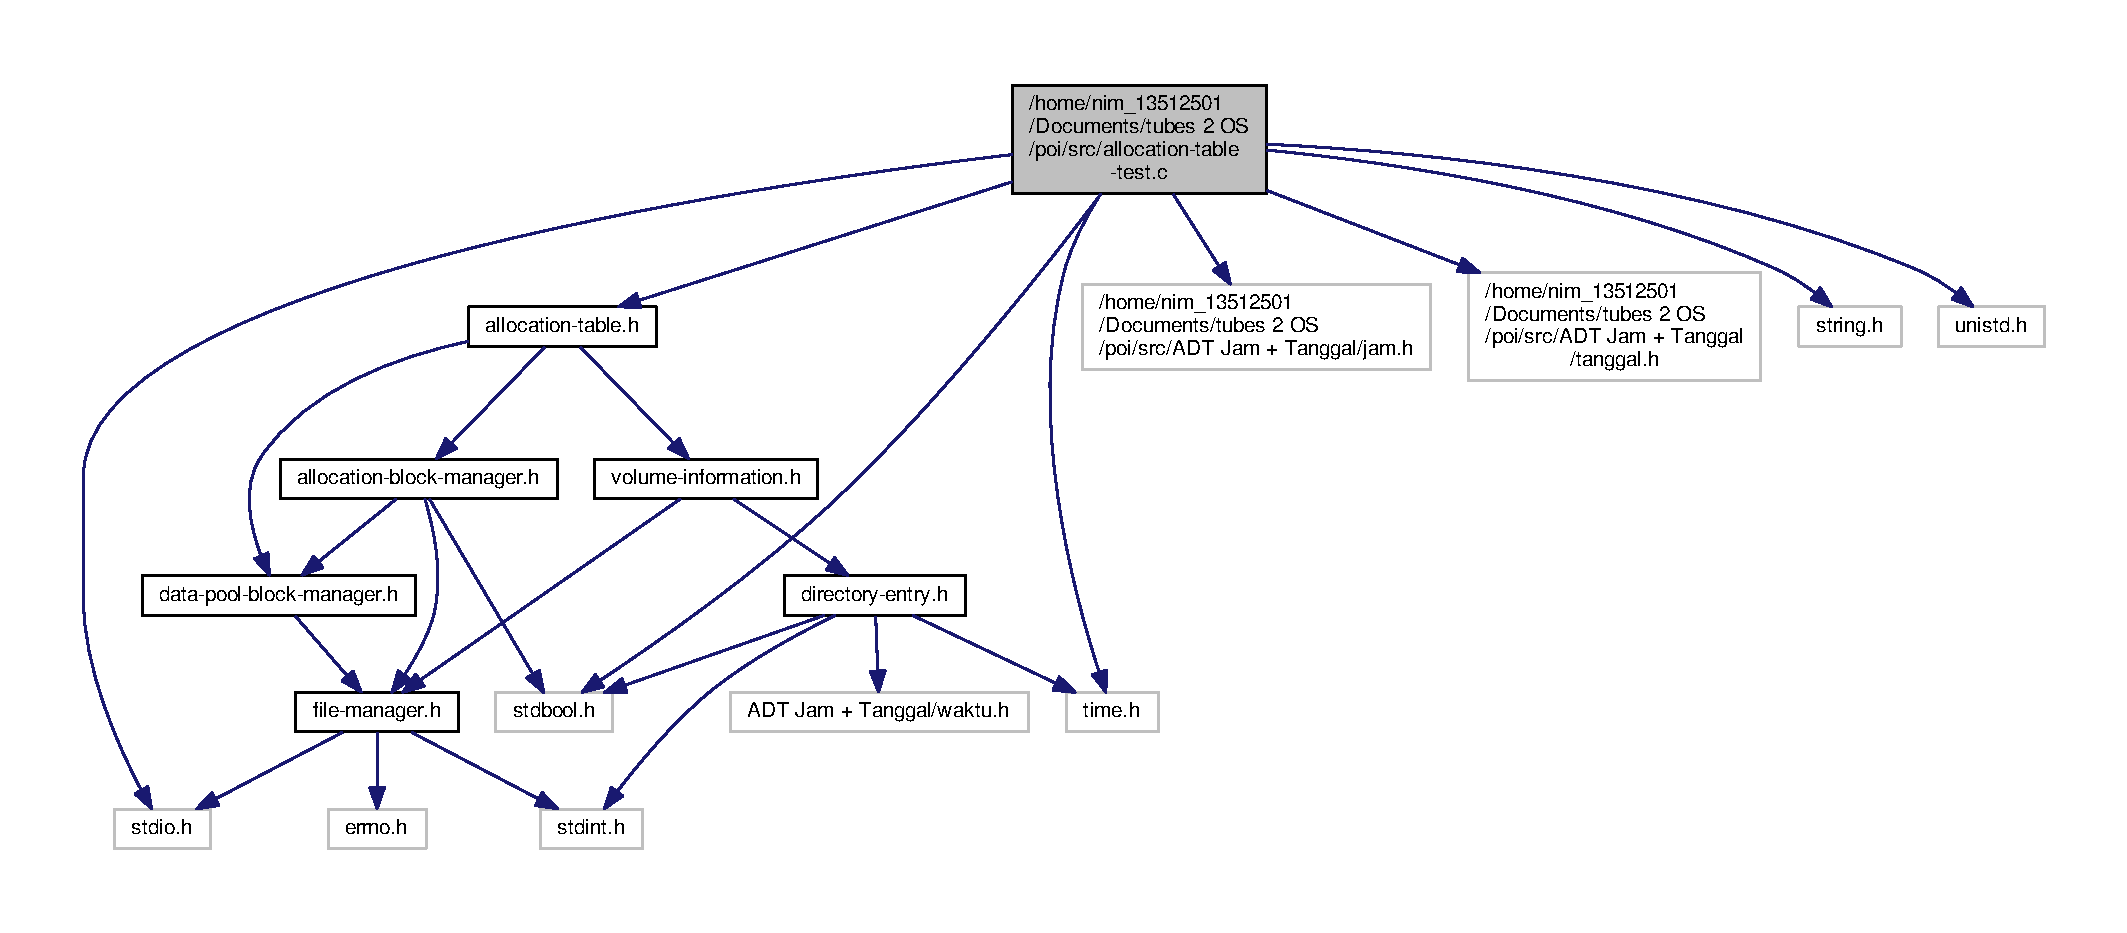
\includegraphics[width=350pt]{allocation-table-test_8c__incl}
\end{center}
\end{figure}
\subsection*{Functions}
\begin{DoxyCompactItemize}
\item 
void \hyperlink{allocation-table-test_8c_a20af25d3b441d1f25e4830ee2173480c}{save\-Alloc\-Table\-Caches} ()
\item 
void \hyperlink{allocation-table-test_8c_ae0bde2314239fb8dbf38c13fee0a68fe}{new\-List\-Test} ()
\item 
void \hyperlink{allocation-table-test_8c_a57b7cb9823d22ea55528c91e219b7dae}{allocate\-After\-Test} ()
\item 
int32\-\_\-t \hyperlink{allocation-table-test_8c_ae8700eb5d460019b20c7bdf4d0b5880b}{insert\-After\-Test} ()
\item 
void \hyperlink{allocation-table-test_8c_ace8f7db6e87db1e1e06efbc9437e58f1}{delete\-List\-Of\-Block\-Test} ()
\item 
void \hyperlink{allocation-table-test_8c_a9126bcf052408b8d8f30110d1a6c7627}{allocate\-After\-Banyak\-Test} ()
\item 
int \hyperlink{allocation-table-test_8c_ae66f6b31b5ad750f1fe042a706a4e3d4}{main} ()
\end{DoxyCompactItemize}
\subsection*{Variables}
\begin{DoxyCompactItemize}
\item 
\hyperlink{data-pool-block-manager_8h_a87e19ab8290bcd76be1c7db1e90cc6f6}{poi\-\_\-data\-\_\-pool\-\_\-block\-\_\-idx\-\_\-t} \hyperlink{allocation-table-test_8c_a24010dade8ebab3f87a48022772cd975}{n}
\item 
\hyperlink{data-pool-block-manager_8h_a87e19ab8290bcd76be1c7db1e90cc6f6}{poi\-\_\-data\-\_\-pool\-\_\-block\-\_\-idx\-\_\-t} \hyperlink{allocation-table-test_8c_a64e8737d2c8316bb6a1c98ea9ccda670}{m}
\end{DoxyCompactItemize}


\subsection{Detailed Description}
berkas penggerak uji untuk \hyperlink{allocation-table-test_8c}{allocation-\/table-\/test.\-c} \begin{DoxyAuthor}{Author}
jang berikoetnja 
\end{DoxyAuthor}


\subsection{Function Documentation}
\hypertarget{allocation-table-test_8c_a9126bcf052408b8d8f30110d1a6c7627}{\index{allocation-\/table-\/test.\-c@{allocation-\/table-\/test.\-c}!allocate\-After\-Banyak\-Test@{allocate\-After\-Banyak\-Test}}
\index{allocate\-After\-Banyak\-Test@{allocate\-After\-Banyak\-Test}!allocation-table-test.c@{allocation-\/table-\/test.\-c}}
\subsubsection[{allocate\-After\-Banyak\-Test}]{\setlength{\rightskip}{0pt plus 5cm}void allocate\-After\-Banyak\-Test (
\begin{DoxyParamCaption}
{}
\end{DoxyParamCaption}
)}}\label{allocation-table-test_8c_a9126bcf052408b8d8f30110d1a6c7627}


Here is the call graph for this function\-:\nopagebreak
\begin{figure}[H]
\begin{center}
\leavevmode
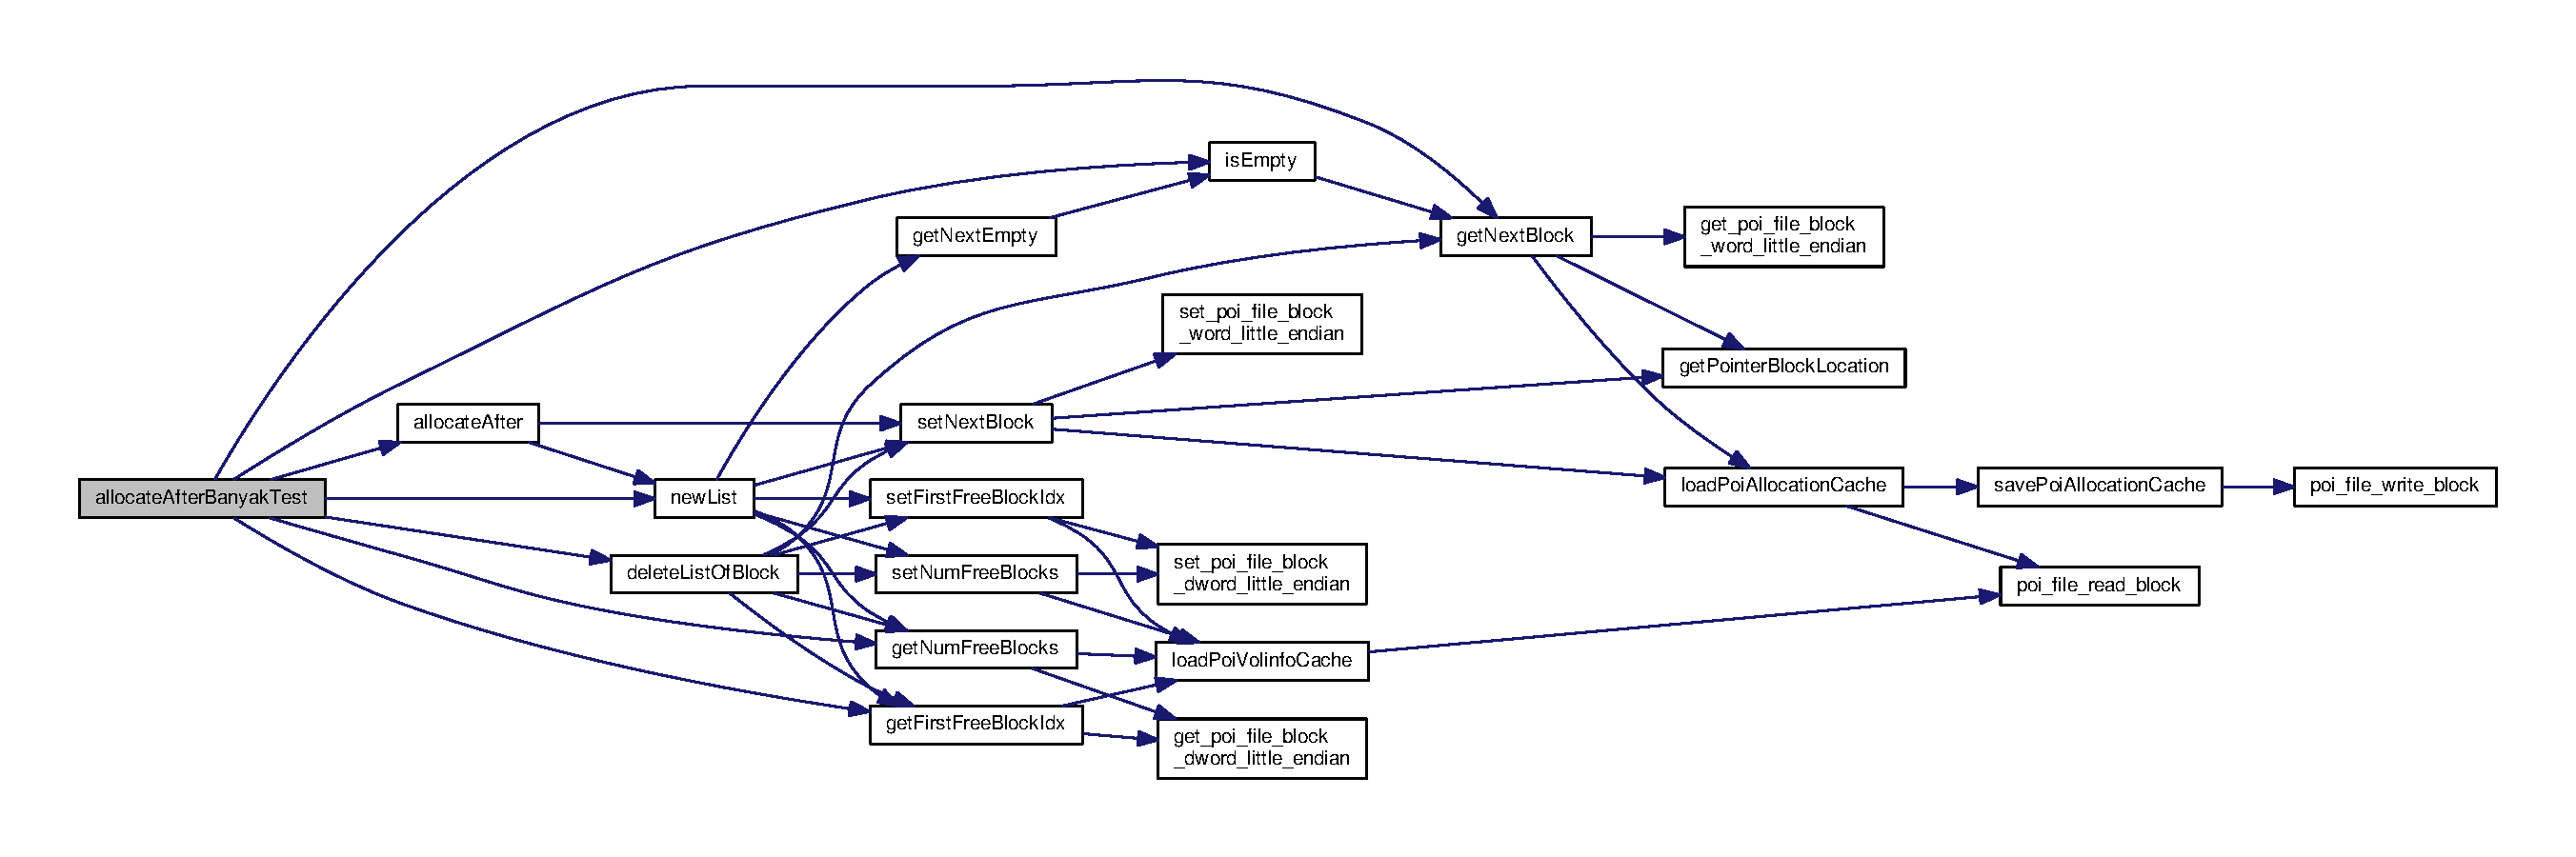
\includegraphics[width=350pt]{allocation-table-test_8c_a9126bcf052408b8d8f30110d1a6c7627_cgraph}
\end{center}
\end{figure}




Here is the caller graph for this function\-:\nopagebreak
\begin{figure}[H]
\begin{center}
\leavevmode
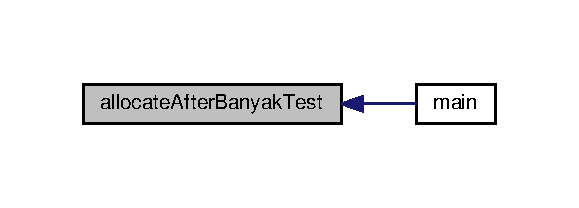
\includegraphics[width=278pt]{allocation-table-test_8c_a9126bcf052408b8d8f30110d1a6c7627_icgraph}
\end{center}
\end{figure}


\hypertarget{allocation-table-test_8c_a57b7cb9823d22ea55528c91e219b7dae}{\index{allocation-\/table-\/test.\-c@{allocation-\/table-\/test.\-c}!allocate\-After\-Test@{allocate\-After\-Test}}
\index{allocate\-After\-Test@{allocate\-After\-Test}!allocation-table-test.c@{allocation-\/table-\/test.\-c}}
\subsubsection[{allocate\-After\-Test}]{\setlength{\rightskip}{0pt plus 5cm}void allocate\-After\-Test (
\begin{DoxyParamCaption}
{}
\end{DoxyParamCaption}
)}}\label{allocation-table-test_8c_a57b7cb9823d22ea55528c91e219b7dae}


Here is the call graph for this function\-:\nopagebreak
\begin{figure}[H]
\begin{center}
\leavevmode
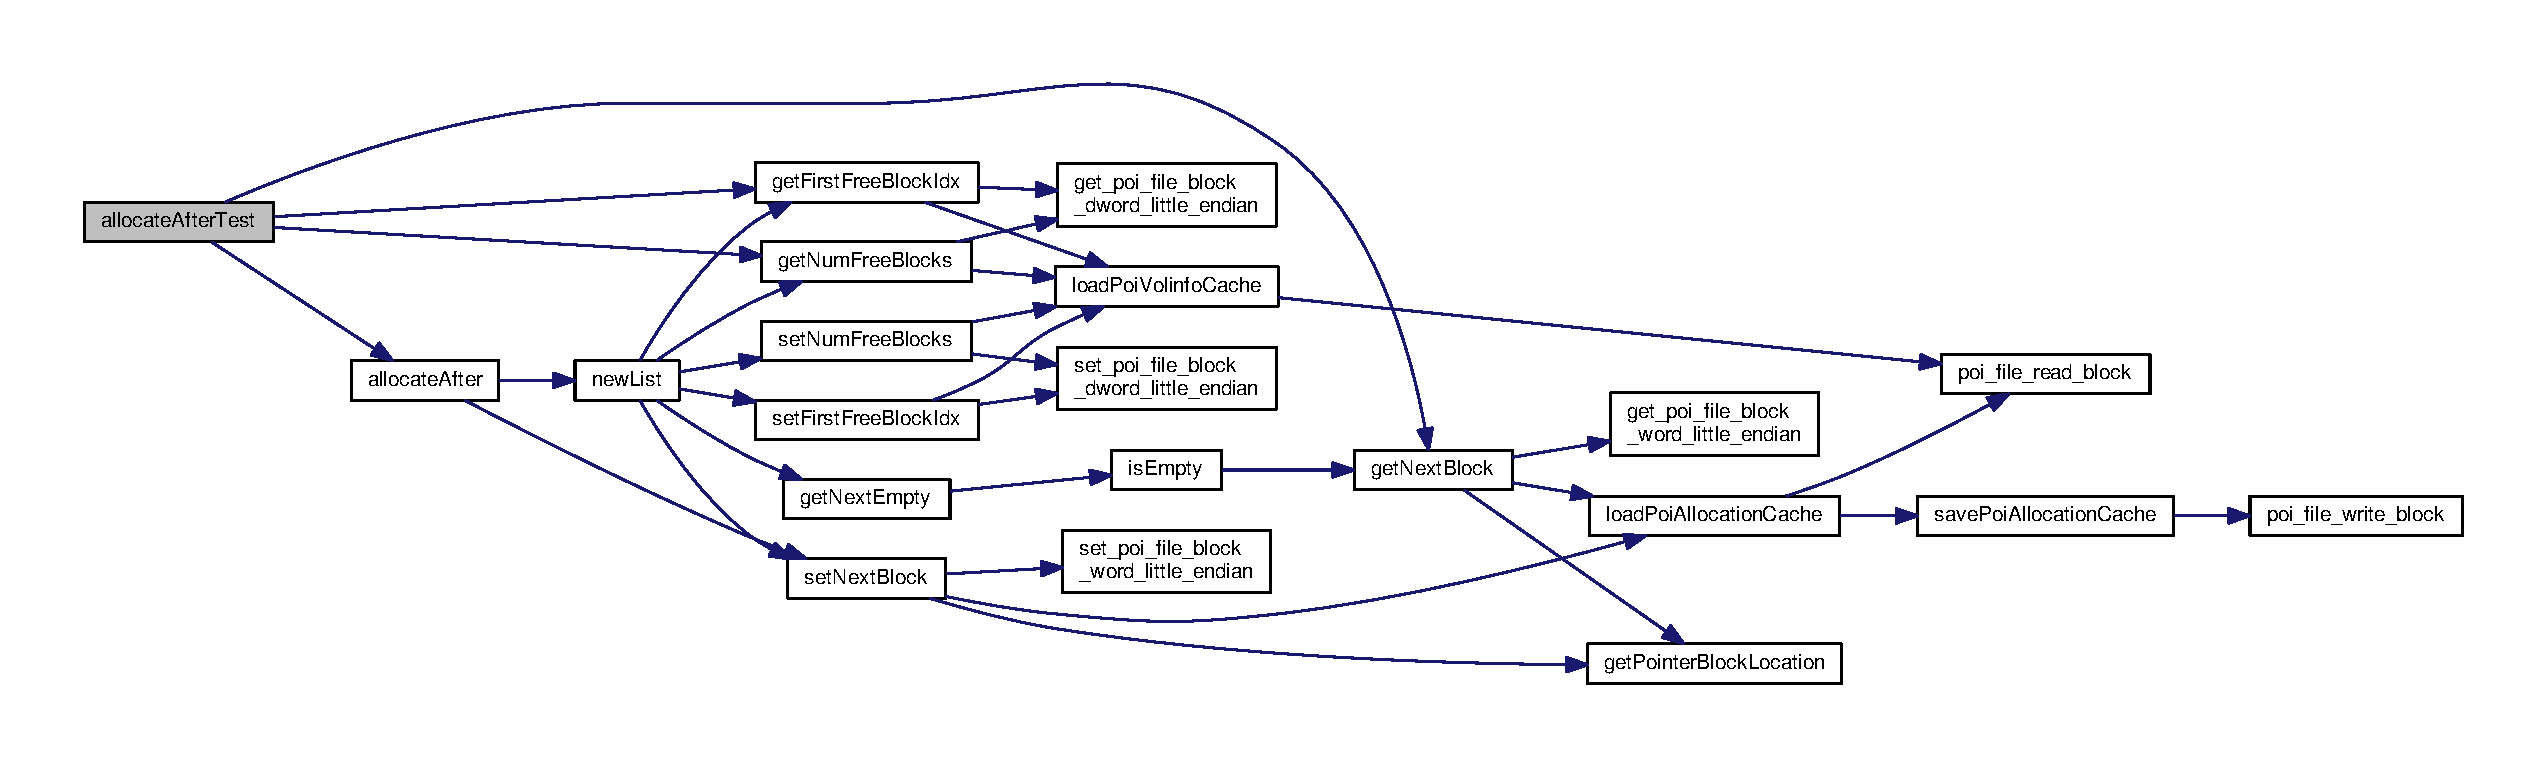
\includegraphics[width=350pt]{allocation-table-test_8c_a57b7cb9823d22ea55528c91e219b7dae_cgraph}
\end{center}
\end{figure}




Here is the caller graph for this function\-:\nopagebreak
\begin{figure}[H]
\begin{center}
\leavevmode
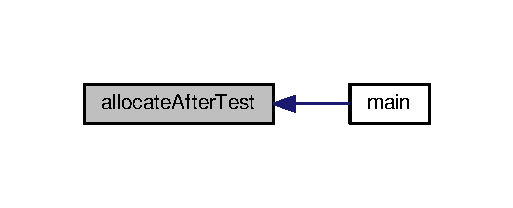
\includegraphics[width=246pt]{allocation-table-test_8c_a57b7cb9823d22ea55528c91e219b7dae_icgraph}
\end{center}
\end{figure}


\hypertarget{allocation-table-test_8c_ace8f7db6e87db1e1e06efbc9437e58f1}{\index{allocation-\/table-\/test.\-c@{allocation-\/table-\/test.\-c}!delete\-List\-Of\-Block\-Test@{delete\-List\-Of\-Block\-Test}}
\index{delete\-List\-Of\-Block\-Test@{delete\-List\-Of\-Block\-Test}!allocation-table-test.c@{allocation-\/table-\/test.\-c}}
\subsubsection[{delete\-List\-Of\-Block\-Test}]{\setlength{\rightskip}{0pt plus 5cm}void delete\-List\-Of\-Block\-Test (
\begin{DoxyParamCaption}
{}
\end{DoxyParamCaption}
)}}\label{allocation-table-test_8c_ace8f7db6e87db1e1e06efbc9437e58f1}


Here is the call graph for this function\-:\nopagebreak
\begin{figure}[H]
\begin{center}
\leavevmode
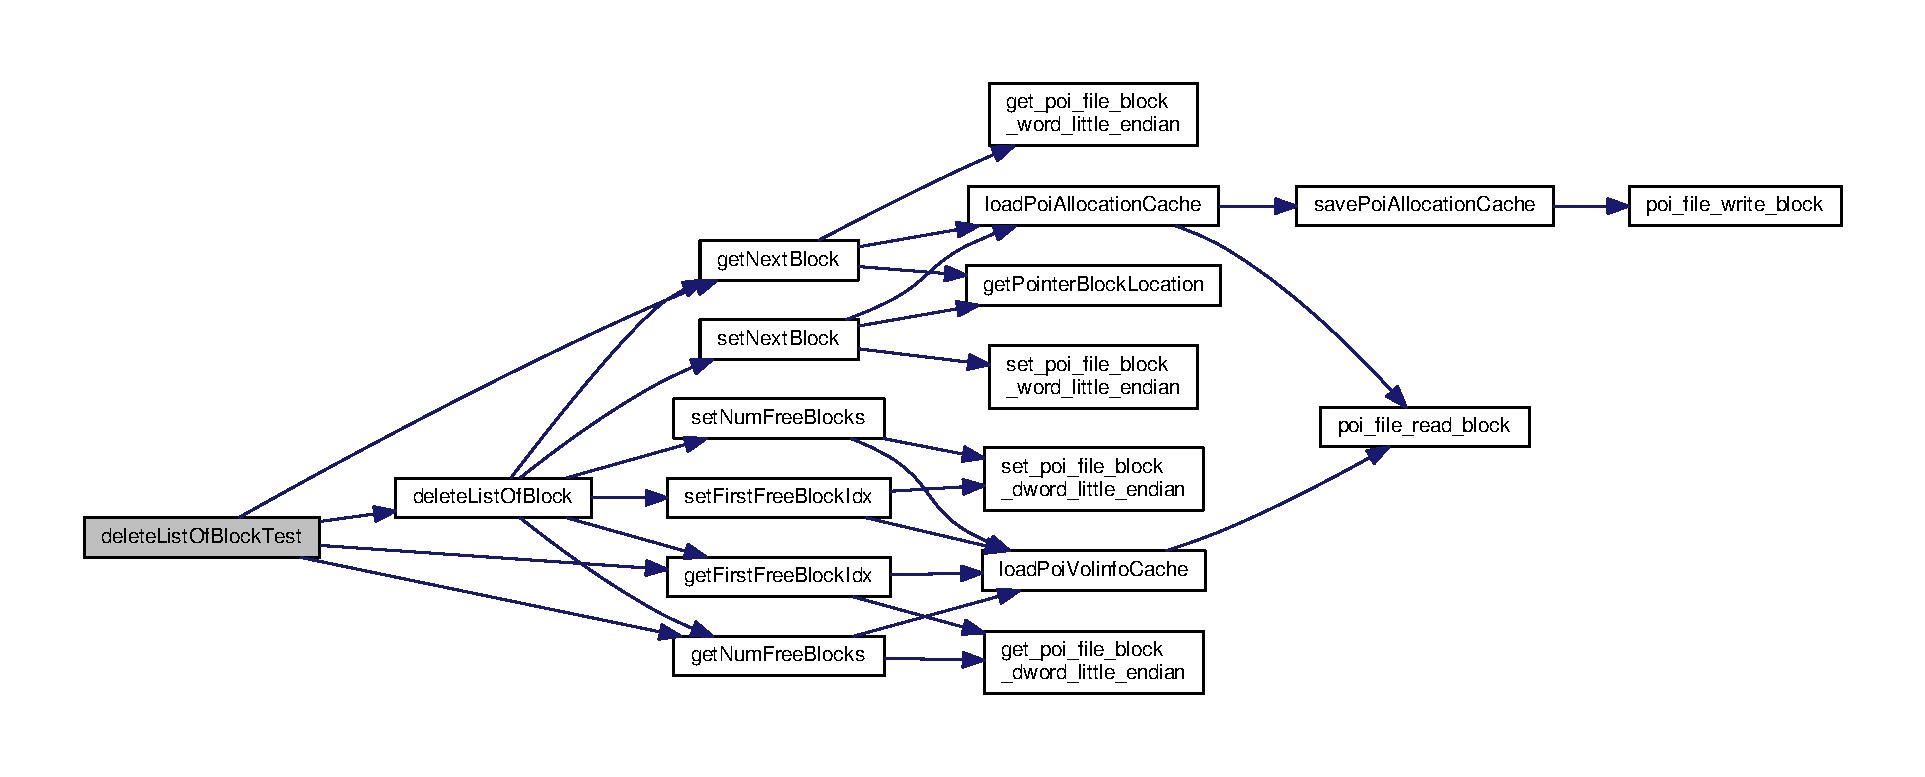
\includegraphics[width=350pt]{allocation-table-test_8c_ace8f7db6e87db1e1e06efbc9437e58f1_cgraph}
\end{center}
\end{figure}




Here is the caller graph for this function\-:\nopagebreak
\begin{figure}[H]
\begin{center}
\leavevmode
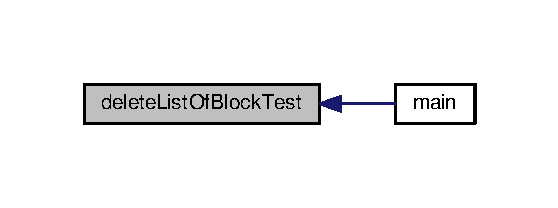
\includegraphics[width=268pt]{allocation-table-test_8c_ace8f7db6e87db1e1e06efbc9437e58f1_icgraph}
\end{center}
\end{figure}


\hypertarget{allocation-table-test_8c_ae8700eb5d460019b20c7bdf4d0b5880b}{\index{allocation-\/table-\/test.\-c@{allocation-\/table-\/test.\-c}!insert\-After\-Test@{insert\-After\-Test}}
\index{insert\-After\-Test@{insert\-After\-Test}!allocation-table-test.c@{allocation-\/table-\/test.\-c}}
\subsubsection[{insert\-After\-Test}]{\setlength{\rightskip}{0pt plus 5cm}int32\-\_\-t insert\-After\-Test (
\begin{DoxyParamCaption}
{}
\end{DoxyParamCaption}
)}}\label{allocation-table-test_8c_ae8700eb5d460019b20c7bdf4d0b5880b}


Here is the call graph for this function\-:\nopagebreak
\begin{figure}[H]
\begin{center}
\leavevmode
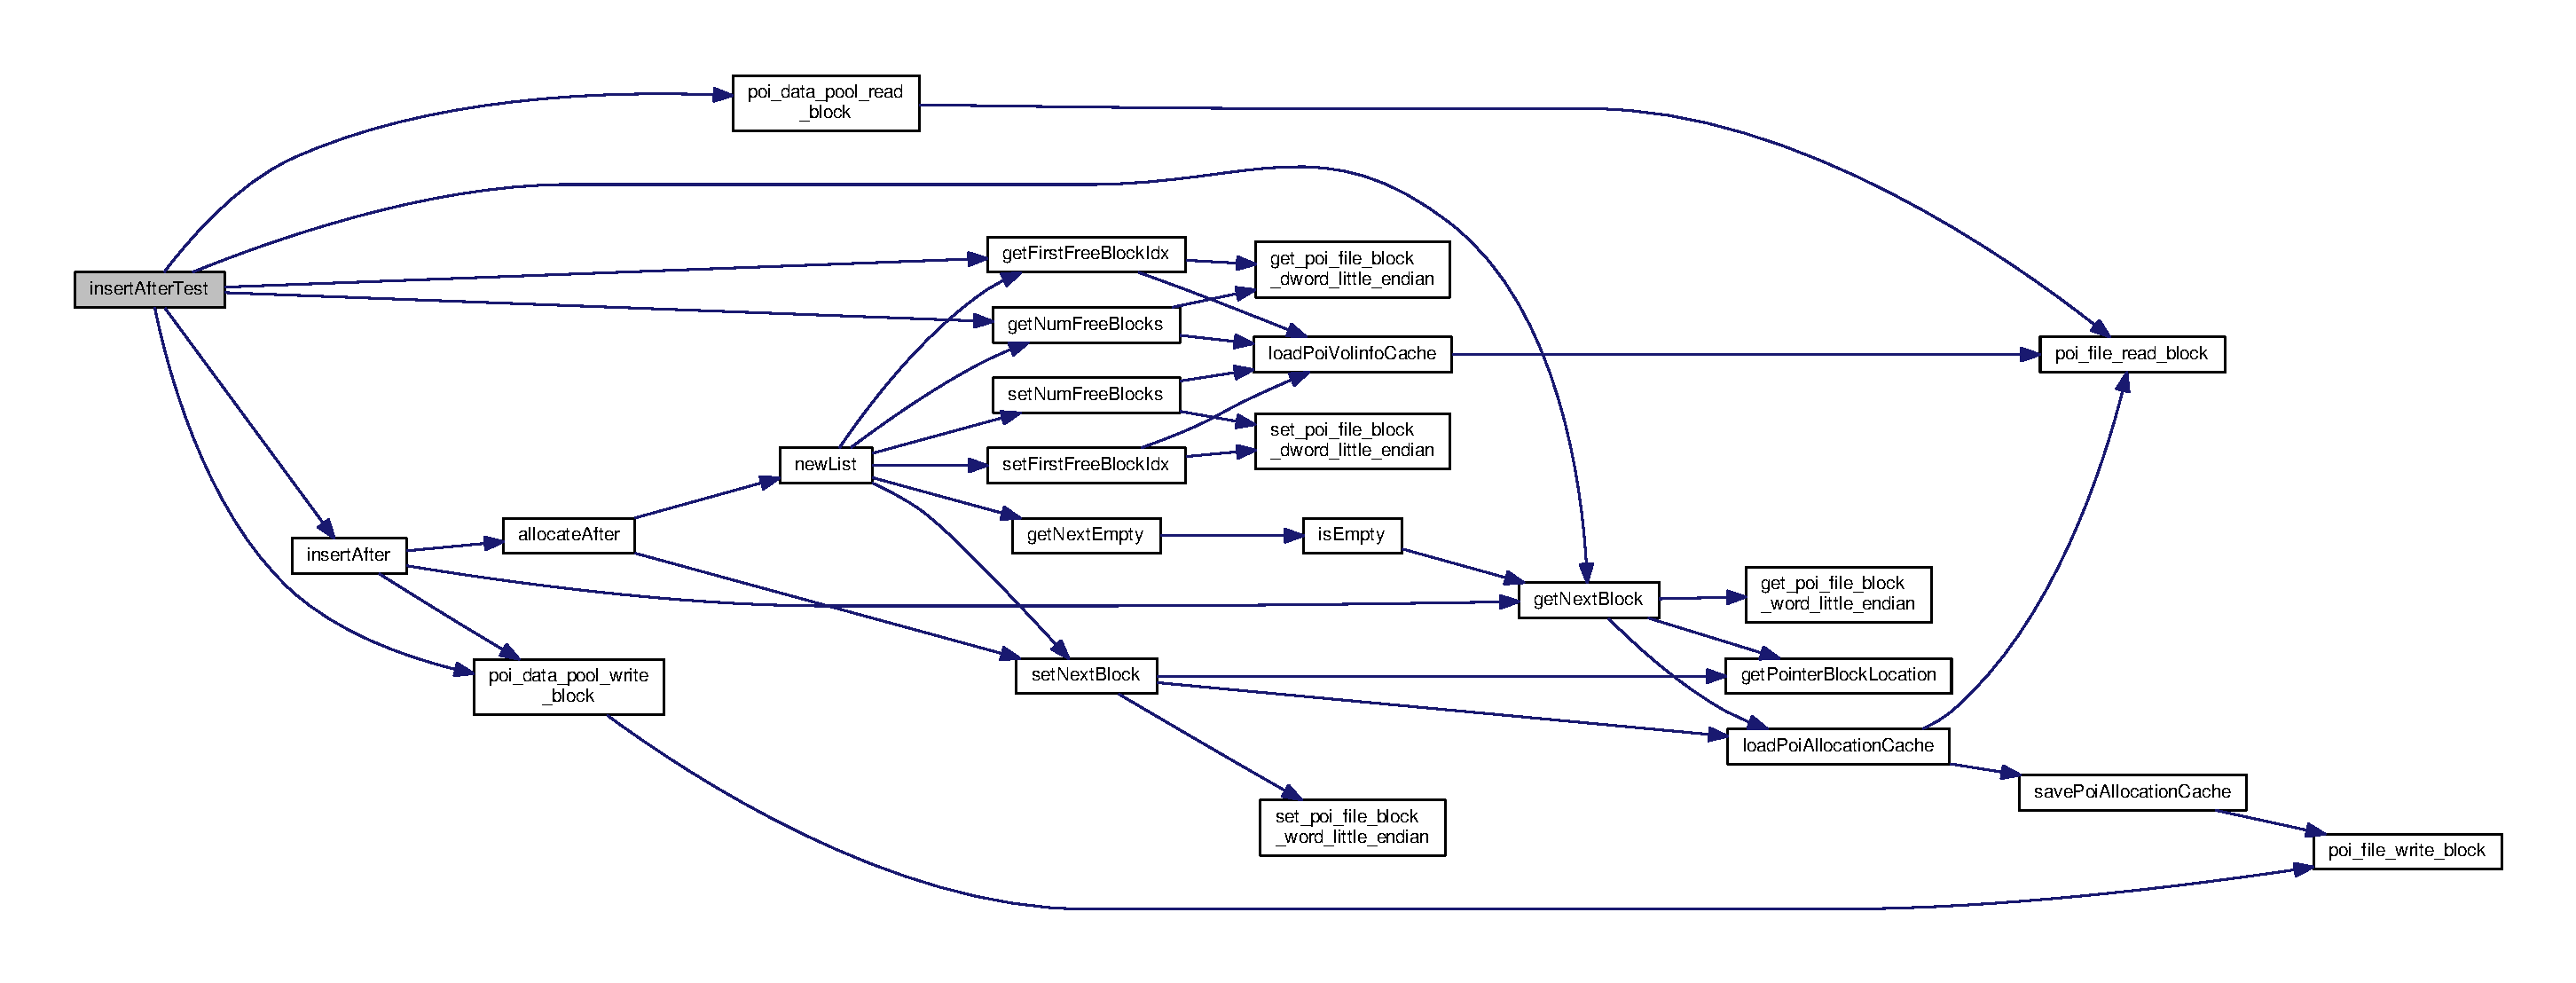
\includegraphics[width=350pt]{allocation-table-test_8c_ae8700eb5d460019b20c7bdf4d0b5880b_cgraph}
\end{center}
\end{figure}




Here is the caller graph for this function\-:\nopagebreak
\begin{figure}[H]
\begin{center}
\leavevmode
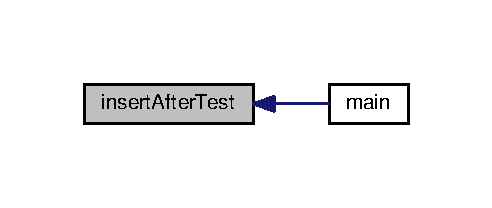
\includegraphics[width=236pt]{allocation-table-test_8c_ae8700eb5d460019b20c7bdf4d0b5880b_icgraph}
\end{center}
\end{figure}


\hypertarget{allocation-table-test_8c_ae66f6b31b5ad750f1fe042a706a4e3d4}{\index{allocation-\/table-\/test.\-c@{allocation-\/table-\/test.\-c}!main@{main}}
\index{main@{main}!allocation-table-test.c@{allocation-\/table-\/test.\-c}}
\subsubsection[{main}]{\setlength{\rightskip}{0pt plus 5cm}int main (
\begin{DoxyParamCaption}
{}
\end{DoxyParamCaption}
)}}\label{allocation-table-test_8c_ae66f6b31b5ad750f1fe042a706a4e3d4}


Here is the call graph for this function\-:\nopagebreak
\begin{figure}[H]
\begin{center}
\leavevmode
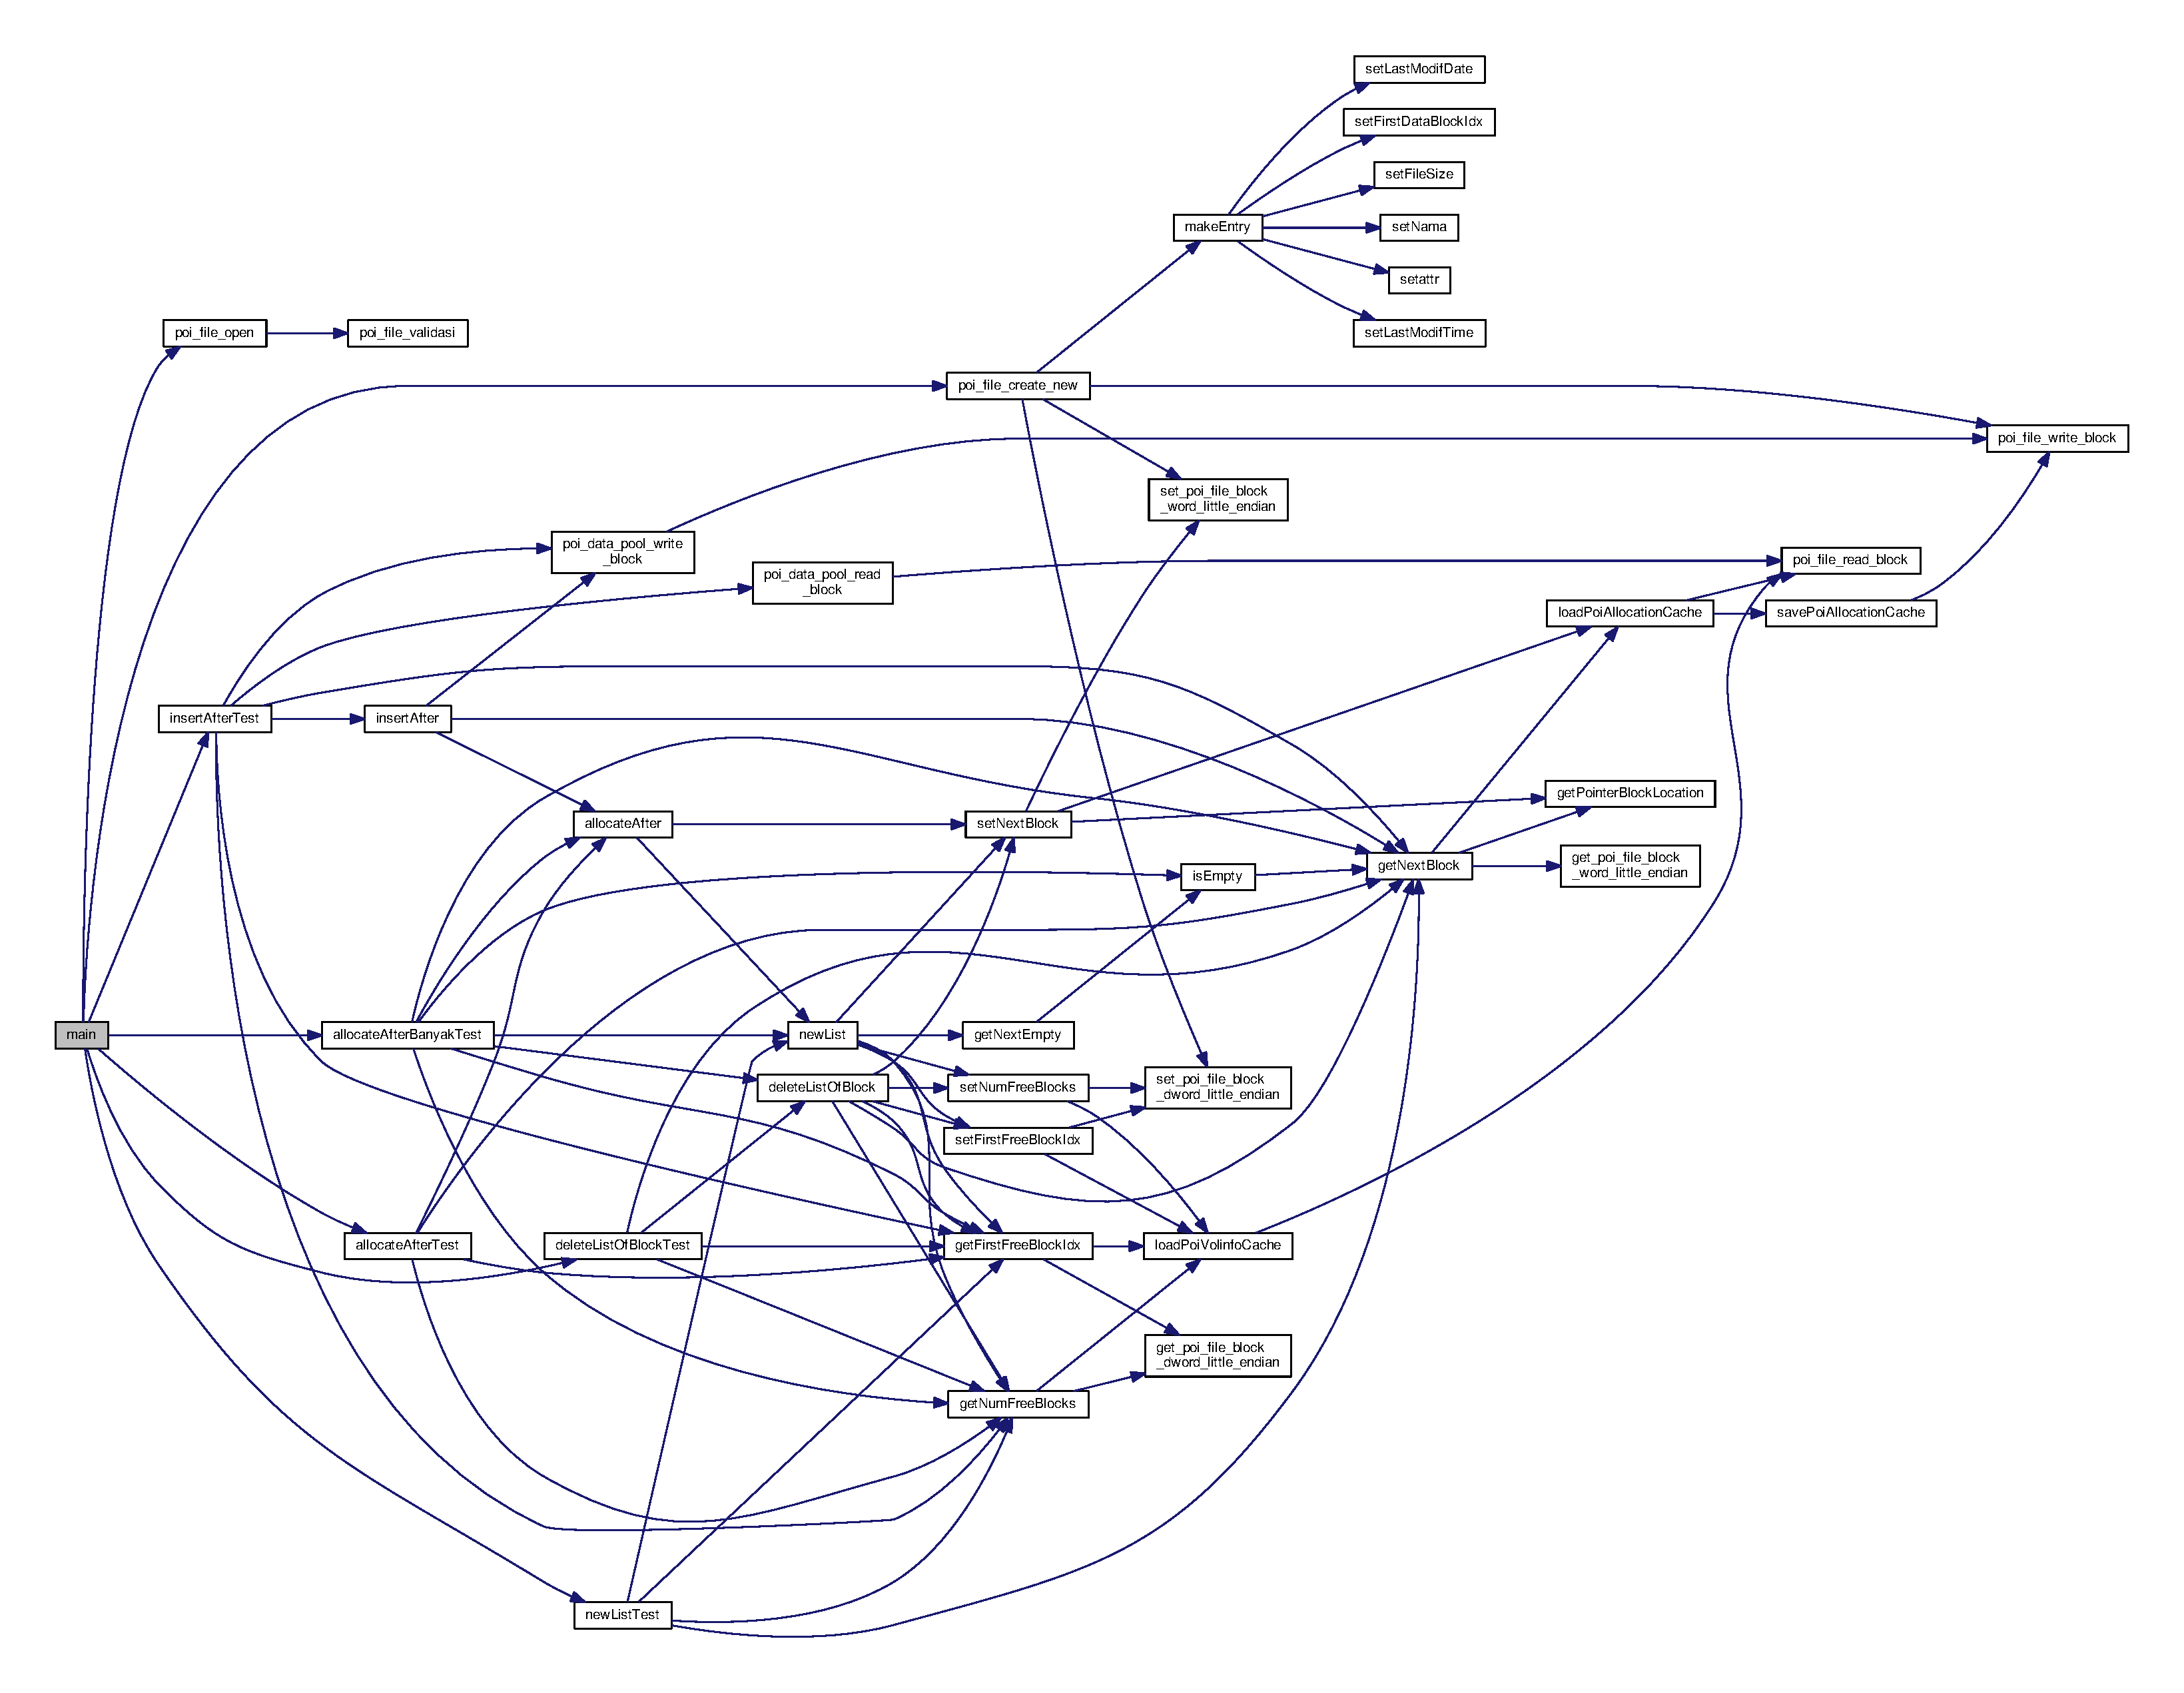
\includegraphics[width=350pt]{allocation-table-test_8c_ae66f6b31b5ad750f1fe042a706a4e3d4_cgraph}
\end{center}
\end{figure}


\hypertarget{allocation-table-test_8c_ae0bde2314239fb8dbf38c13fee0a68fe}{\index{allocation-\/table-\/test.\-c@{allocation-\/table-\/test.\-c}!new\-List\-Test@{new\-List\-Test}}
\index{new\-List\-Test@{new\-List\-Test}!allocation-table-test.c@{allocation-\/table-\/test.\-c}}
\subsubsection[{new\-List\-Test}]{\setlength{\rightskip}{0pt plus 5cm}void new\-List\-Test (
\begin{DoxyParamCaption}
{}
\end{DoxyParamCaption}
)}}\label{allocation-table-test_8c_ae0bde2314239fb8dbf38c13fee0a68fe}


Here is the call graph for this function\-:\nopagebreak
\begin{figure}[H]
\begin{center}
\leavevmode
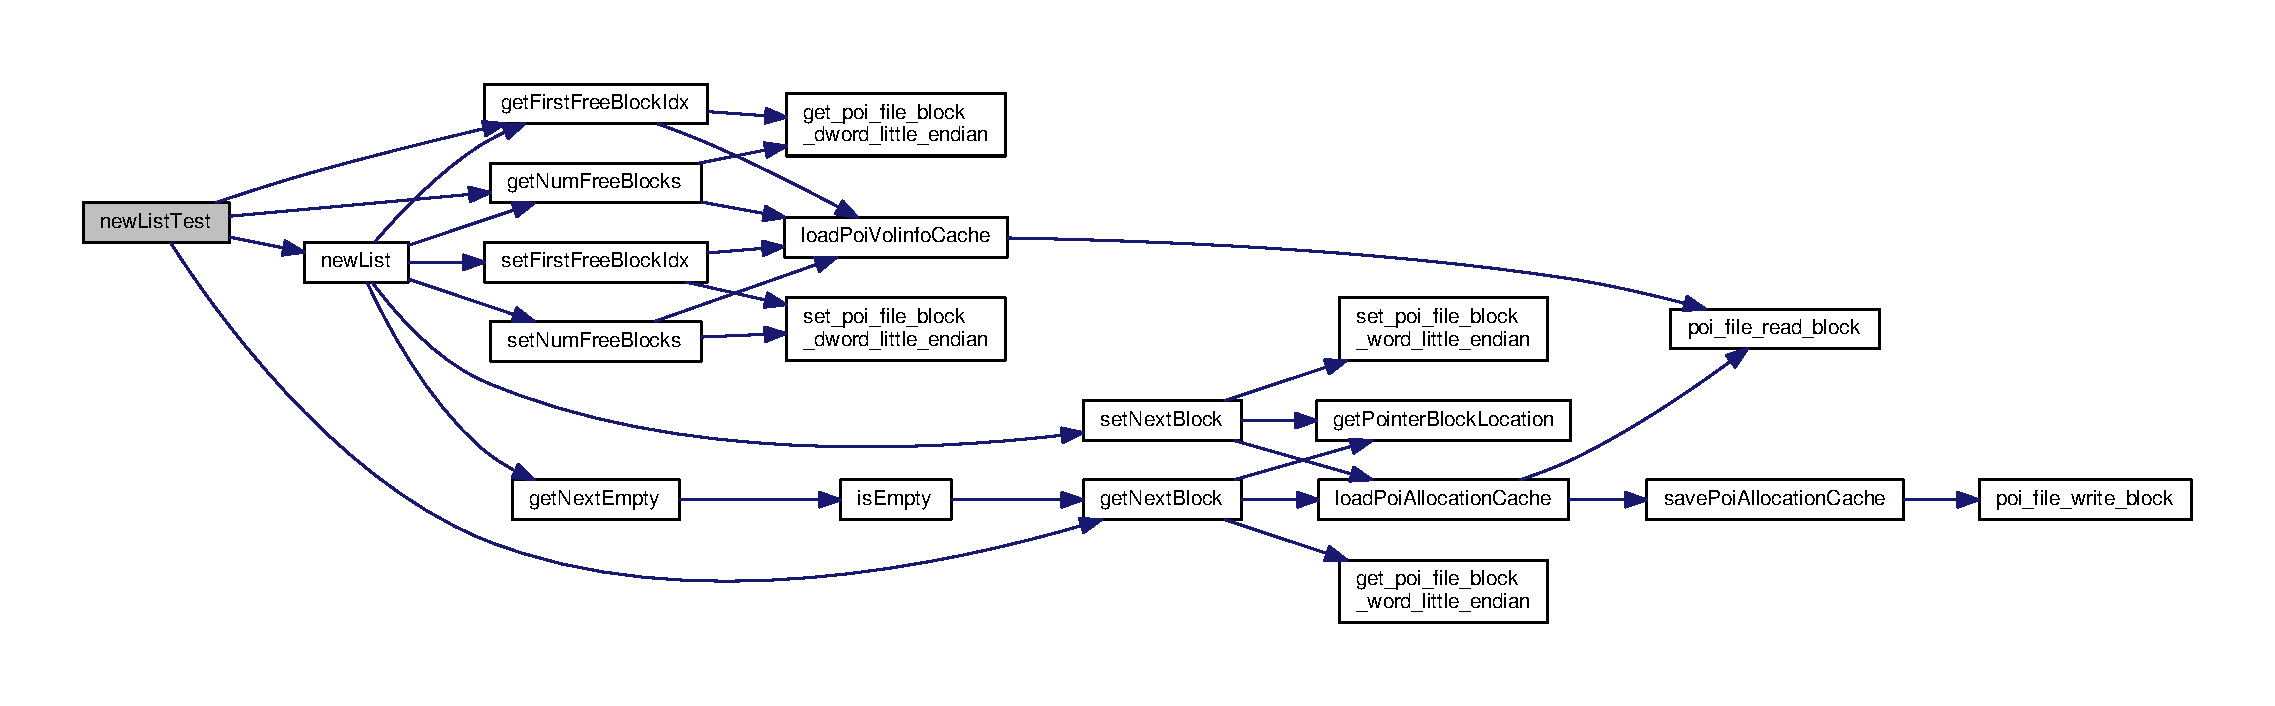
\includegraphics[width=350pt]{allocation-table-test_8c_ae0bde2314239fb8dbf38c13fee0a68fe_cgraph}
\end{center}
\end{figure}




Here is the caller graph for this function\-:\nopagebreak
\begin{figure}[H]
\begin{center}
\leavevmode
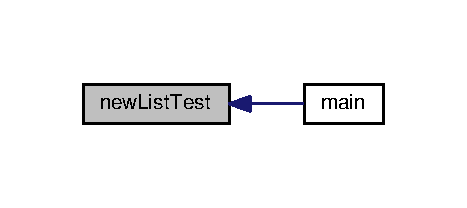
\includegraphics[width=224pt]{allocation-table-test_8c_ae0bde2314239fb8dbf38c13fee0a68fe_icgraph}
\end{center}
\end{figure}


\hypertarget{allocation-table-test_8c_a20af25d3b441d1f25e4830ee2173480c}{\index{allocation-\/table-\/test.\-c@{allocation-\/table-\/test.\-c}!save\-Alloc\-Table\-Caches@{save\-Alloc\-Table\-Caches}}
\index{save\-Alloc\-Table\-Caches@{save\-Alloc\-Table\-Caches}!allocation-table-test.c@{allocation-\/table-\/test.\-c}}
\subsubsection[{save\-Alloc\-Table\-Caches}]{\setlength{\rightskip}{0pt plus 5cm}void save\-Alloc\-Table\-Caches (
\begin{DoxyParamCaption}
{}
\end{DoxyParamCaption}
)}}\label{allocation-table-test_8c_a20af25d3b441d1f25e4830ee2173480c}


Here is the caller graph for this function\-:\nopagebreak
\begin{figure}[H]
\begin{center}
\leavevmode
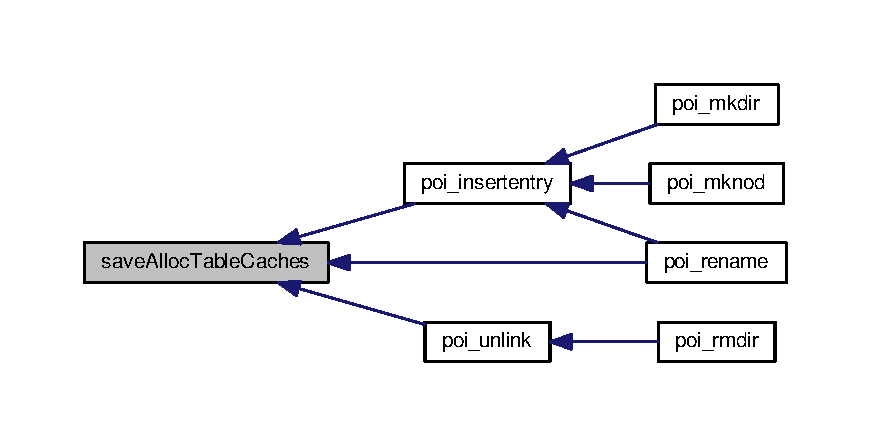
\includegraphics[width=350pt]{allocation-table-test_8c_a20af25d3b441d1f25e4830ee2173480c_icgraph}
\end{center}
\end{figure}




\subsection{Variable Documentation}
\hypertarget{allocation-table-test_8c_a64e8737d2c8316bb6a1c98ea9ccda670}{\index{allocation-\/table-\/test.\-c@{allocation-\/table-\/test.\-c}!m@{m}}
\index{m@{m}!allocation-table-test.c@{allocation-\/table-\/test.\-c}}
\subsubsection[{m}]{\setlength{\rightskip}{0pt plus 5cm}{\bf poi\-\_\-data\-\_\-pool\-\_\-block\-\_\-idx\-\_\-t} m}}\label{allocation-table-test_8c_a64e8737d2c8316bb6a1c98ea9ccda670}
\hypertarget{allocation-table-test_8c_a24010dade8ebab3f87a48022772cd975}{\index{allocation-\/table-\/test.\-c@{allocation-\/table-\/test.\-c}!n@{n}}
\index{n@{n}!allocation-table-test.c@{allocation-\/table-\/test.\-c}}
\subsubsection[{n}]{\setlength{\rightskip}{0pt plus 5cm}{\bf poi\-\_\-data\-\_\-pool\-\_\-block\-\_\-idx\-\_\-t} n}}\label{allocation-table-test_8c_a24010dade8ebab3f87a48022772cd975}

\hypertarget{allocation-table_8c}{\section{/home/nim\-\_\-13512501/\-Documents/tubes 2 O\-S/poi/src/allocation-\/table.c File Reference}
\label{allocation-table_8c}\index{/home/nim\-\_\-13512501/\-Documents/tubes 2 O\-S/poi/src/allocation-\/table.\-c@{/home/nim\-\_\-13512501/\-Documents/tubes 2 O\-S/poi/src/allocation-\/table.\-c}}
}


mengatur seluruh senarai berkait alokasi berkas.  


{\ttfamily \#include \char`\"{}allocation-\/table.\-h\char`\"{}}\\*
Include dependency graph for allocation-\/table.c\-:\nopagebreak
\begin{figure}[H]
\begin{center}
\leavevmode
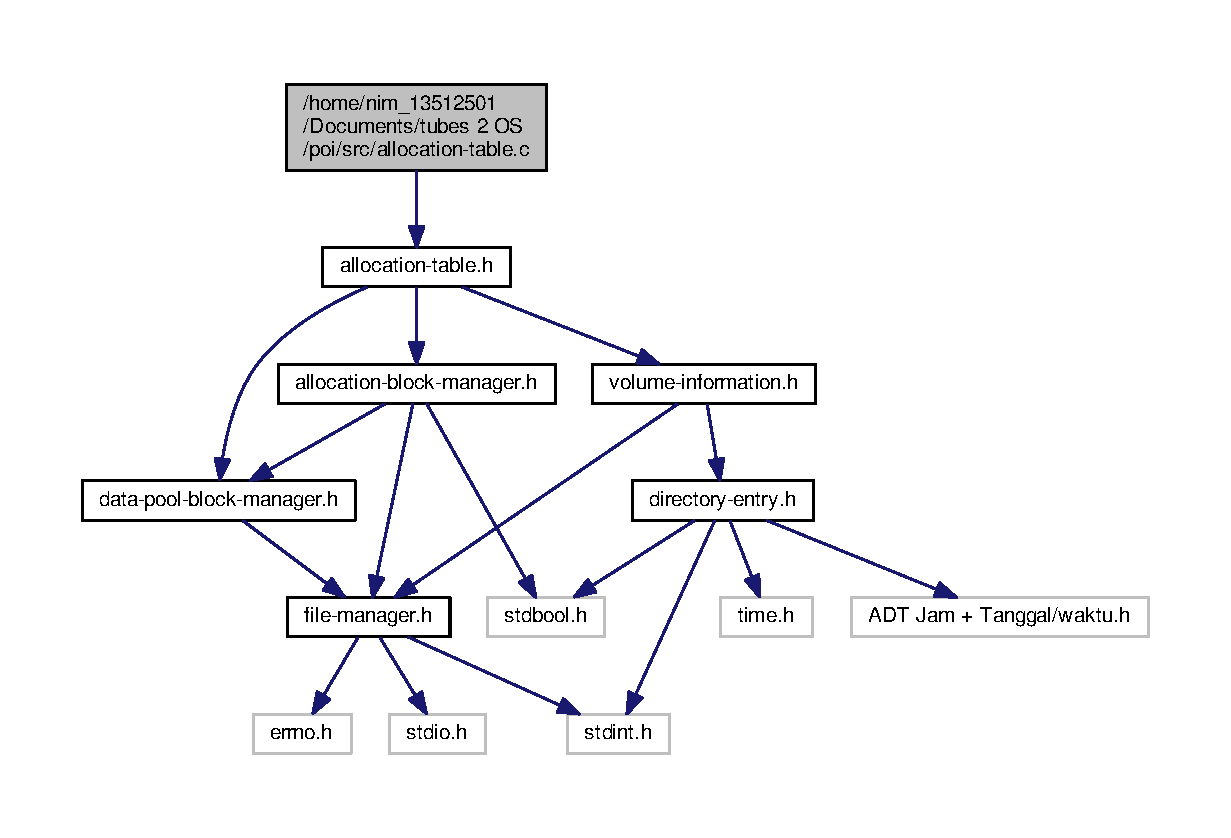
\includegraphics[width=350pt]{allocation-table_8c__incl}
\end{center}
\end{figure}
\subsection*{Macros}
\begin{DoxyCompactItemize}
\item 
\#define \hyperlink{allocation-table_8c_afc5318de31f175f755f75812b44051c6}{allocation\-\_\-table\-\_\-c}
\end{DoxyCompactItemize}
\subsection*{Functions}
\begin{DoxyCompactItemize}
\item 
void \hyperlink{allocation-table_8c_a20af25d3b441d1f25e4830ee2173480c}{save\-Alloc\-Table\-Caches} ()
\item 
int32\-\_\-t \hyperlink{allocation-table_8c_ada2e09277dd8e97a2b2b75484b738126}{new\-List} (\hyperlink{data-pool-block-manager_8h_a87e19ab8290bcd76be1c7db1e90cc6f6}{poi\-\_\-data\-\_\-pool\-\_\-block\-\_\-idx\-\_\-t} $\ast$\hyperlink{allocation-table-test_8c_a24010dade8ebab3f87a48022772cd975}{n})
\item 
int32\-\_\-t \hyperlink{allocation-table_8c_a89ea9558bd50decb1bbbf85e569fe6c5}{allocate\-After} (\hyperlink{data-pool-block-manager_8h_a87e19ab8290bcd76be1c7db1e90cc6f6}{poi\-\_\-data\-\_\-pool\-\_\-block\-\_\-idx\-\_\-t} \hyperlink{allocation-table-test_8c_a24010dade8ebab3f87a48022772cd975}{n})
\item 
int32\-\_\-t \hyperlink{allocation-table_8c_a6de48f9bdf37e8005b9973a75d07633a}{insert\-After} (\hyperlink{data-pool-block-manager_8h_a87e19ab8290bcd76be1c7db1e90cc6f6}{poi\-\_\-data\-\_\-pool\-\_\-block\-\_\-idx\-\_\-t} \hyperlink{allocation-table-test_8c_a24010dade8ebab3f87a48022772cd975}{n}, \hyperlink{structpoi__file__block}{poi\-\_\-file\-\_\-block} blk)
\item 
void \hyperlink{allocation-table_8c_a8d703df55ad80bb8fb1177a0542065b6}{delete\-List\-Of\-Block} (\hyperlink{data-pool-block-manager_8h_a87e19ab8290bcd76be1c7db1e90cc6f6}{poi\-\_\-data\-\_\-pool\-\_\-block\-\_\-idx\-\_\-t} \hyperlink{allocation-table-test_8c_a24010dade8ebab3f87a48022772cd975}{n})
\item 
void \hyperlink{allocation-table_8c_a986965542b07562f2f205f9d68043a9c}{truncate\-List} (\hyperlink{data-pool-block-manager_8h_a87e19ab8290bcd76be1c7db1e90cc6f6}{poi\-\_\-data\-\_\-pool\-\_\-block\-\_\-idx\-\_\-t} \hyperlink{allocation-table-test_8c_a24010dade8ebab3f87a48022772cd975}{n})
\end{DoxyCompactItemize}


\subsection{Detailed Description}
mengatur seluruh senarai berkait alokasi berkas. \begin{DoxyAuthor}{Author}
jang berikoetnja Memperhitungkan juga ruang kosong. Bila ingin aman dengan perhitungan ruang kosong, panggil ini dan tidak langsung ke \hyperlink{allocation-block-manager_8h}{allocation-\/block-\/manager.\-h} dalam hal manipulasi senarai. (dalam hal pengambilan saja, aman untuk mengambil langsung ke \hyperlink{allocation-block-manager_8h}{allocation-\/block-\/manager.\-h}) Menggunakan cache dari allocation-\/table dan volume-\/information. Setiap akhir manipulasi harus memanggil \hyperlink{allocation-table_8c_a20af25d3b441d1f25e4830ee2173480c}{save\-Alloc\-Table\-Caches()} 
\end{DoxyAuthor}


\subsection{Macro Definition Documentation}
\hypertarget{allocation-table_8c_afc5318de31f175f755f75812b44051c6}{\index{allocation-\/table.\-c@{allocation-\/table.\-c}!allocation\-\_\-table\-\_\-c@{allocation\-\_\-table\-\_\-c}}
\index{allocation\-\_\-table\-\_\-c@{allocation\-\_\-table\-\_\-c}!allocation-table.c@{allocation-\/table.\-c}}
\subsubsection[{allocation\-\_\-table\-\_\-c}]{\setlength{\rightskip}{0pt plus 5cm}\#define allocation\-\_\-table\-\_\-c}}\label{allocation-table_8c_afc5318de31f175f755f75812b44051c6}


\subsection{Function Documentation}
\hypertarget{allocation-table_8c_a89ea9558bd50decb1bbbf85e569fe6c5}{\index{allocation-\/table.\-c@{allocation-\/table.\-c}!allocate\-After@{allocate\-After}}
\index{allocate\-After@{allocate\-After}!allocation-table.c@{allocation-\/table.\-c}}
\subsubsection[{allocate\-After}]{\setlength{\rightskip}{0pt plus 5cm}int32\-\_\-t allocate\-After (
\begin{DoxyParamCaption}
\item[{{\bf poi\-\_\-data\-\_\-pool\-\_\-block\-\_\-idx\-\_\-t}}]{n}
\end{DoxyParamCaption}
)}}\label{allocation-table_8c_a89ea9558bd50decb1bbbf85e569fe6c5}


Here is the call graph for this function\-:\nopagebreak
\begin{figure}[H]
\begin{center}
\leavevmode
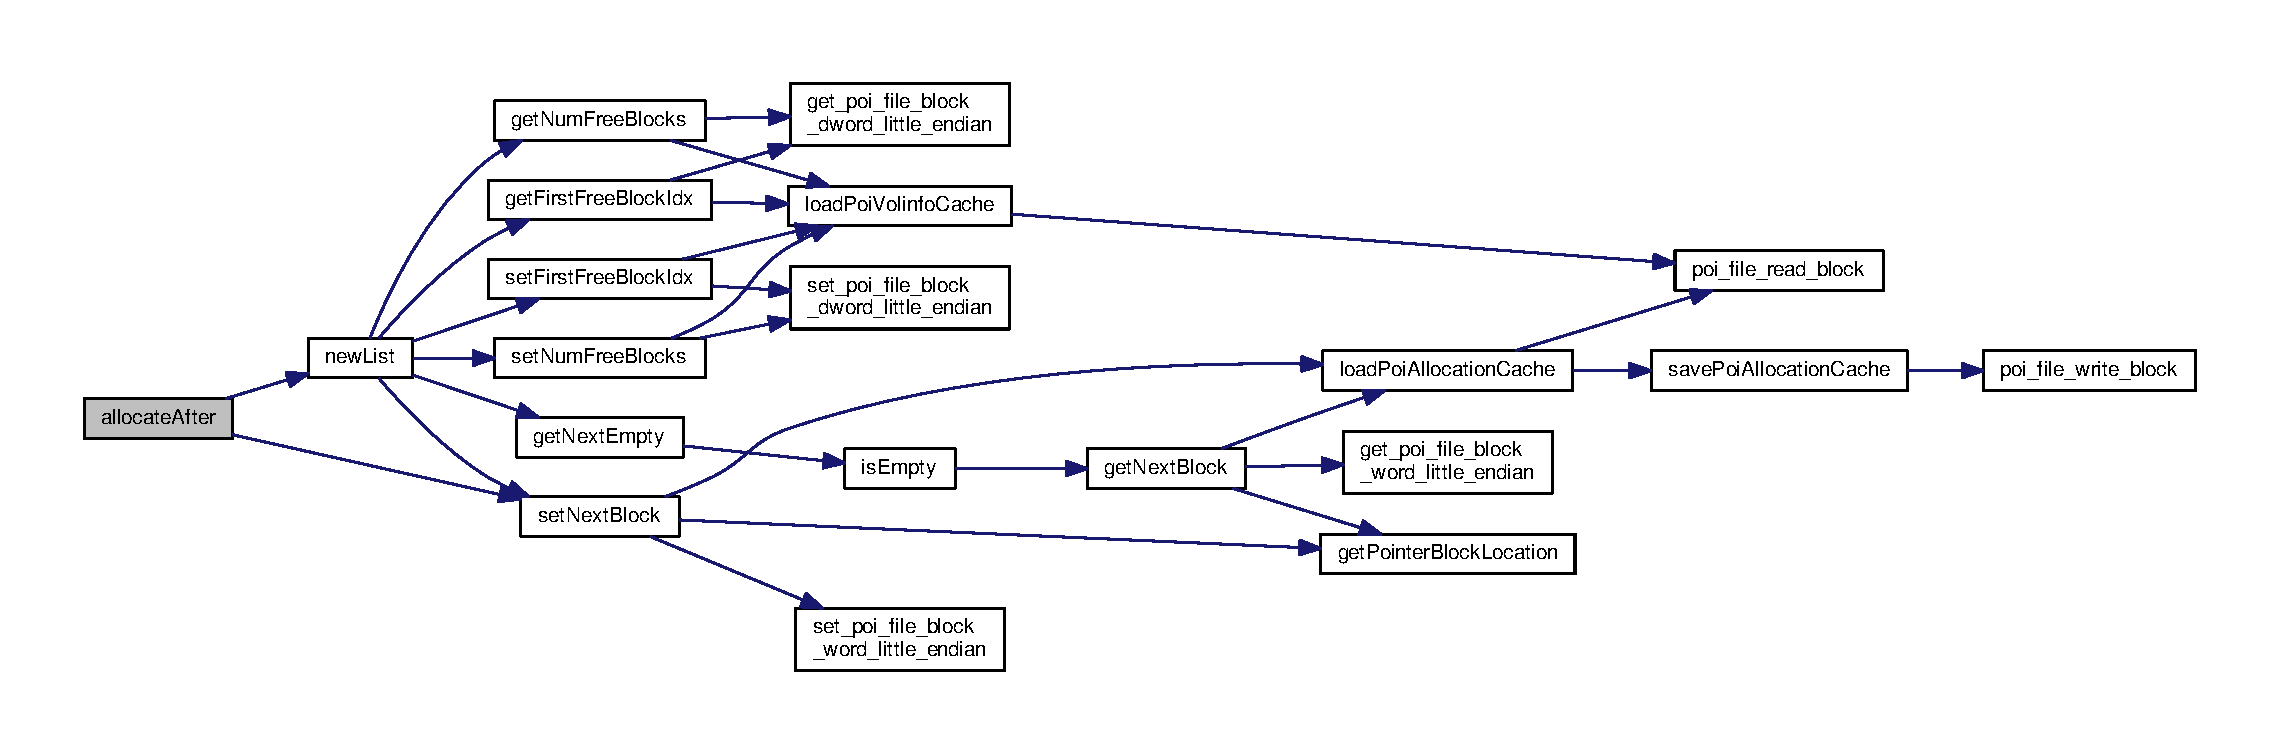
\includegraphics[width=350pt]{allocation-table_8c_a89ea9558bd50decb1bbbf85e569fe6c5_cgraph}
\end{center}
\end{figure}




Here is the caller graph for this function\-:\nopagebreak
\begin{figure}[H]
\begin{center}
\leavevmode
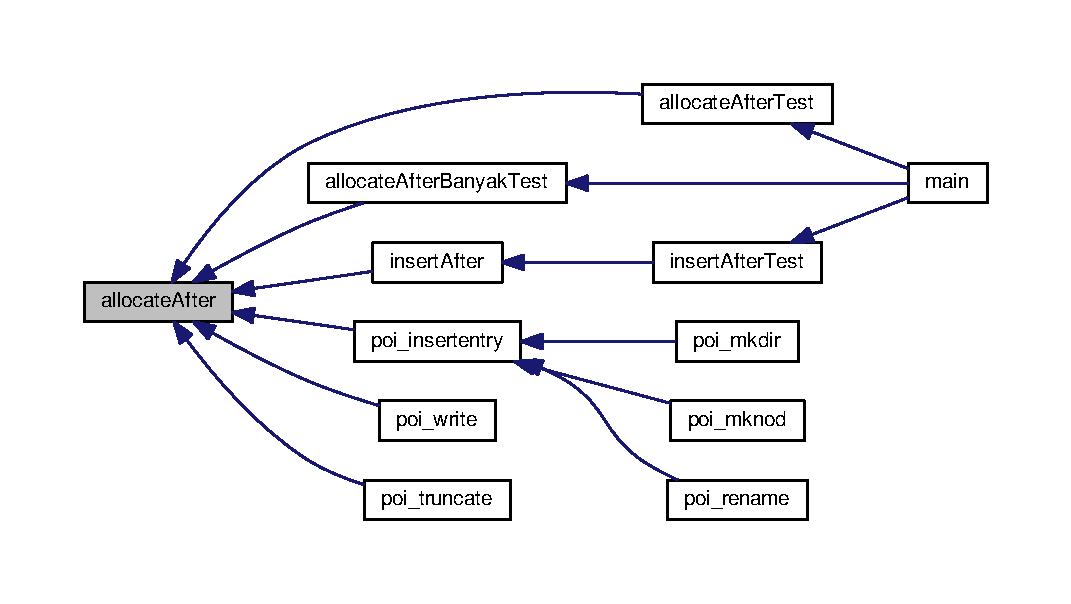
\includegraphics[width=350pt]{allocation-table_8c_a89ea9558bd50decb1bbbf85e569fe6c5_icgraph}
\end{center}
\end{figure}


\hypertarget{allocation-table_8c_a8d703df55ad80bb8fb1177a0542065b6}{\index{allocation-\/table.\-c@{allocation-\/table.\-c}!delete\-List\-Of\-Block@{delete\-List\-Of\-Block}}
\index{delete\-List\-Of\-Block@{delete\-List\-Of\-Block}!allocation-table.c@{allocation-\/table.\-c}}
\subsubsection[{delete\-List\-Of\-Block}]{\setlength{\rightskip}{0pt plus 5cm}void delete\-List\-Of\-Block (
\begin{DoxyParamCaption}
\item[{{\bf poi\-\_\-data\-\_\-pool\-\_\-block\-\_\-idx\-\_\-t}}]{n}
\end{DoxyParamCaption}
)}}\label{allocation-table_8c_a8d703df55ad80bb8fb1177a0542065b6}


Here is the call graph for this function\-:\nopagebreak
\begin{figure}[H]
\begin{center}
\leavevmode
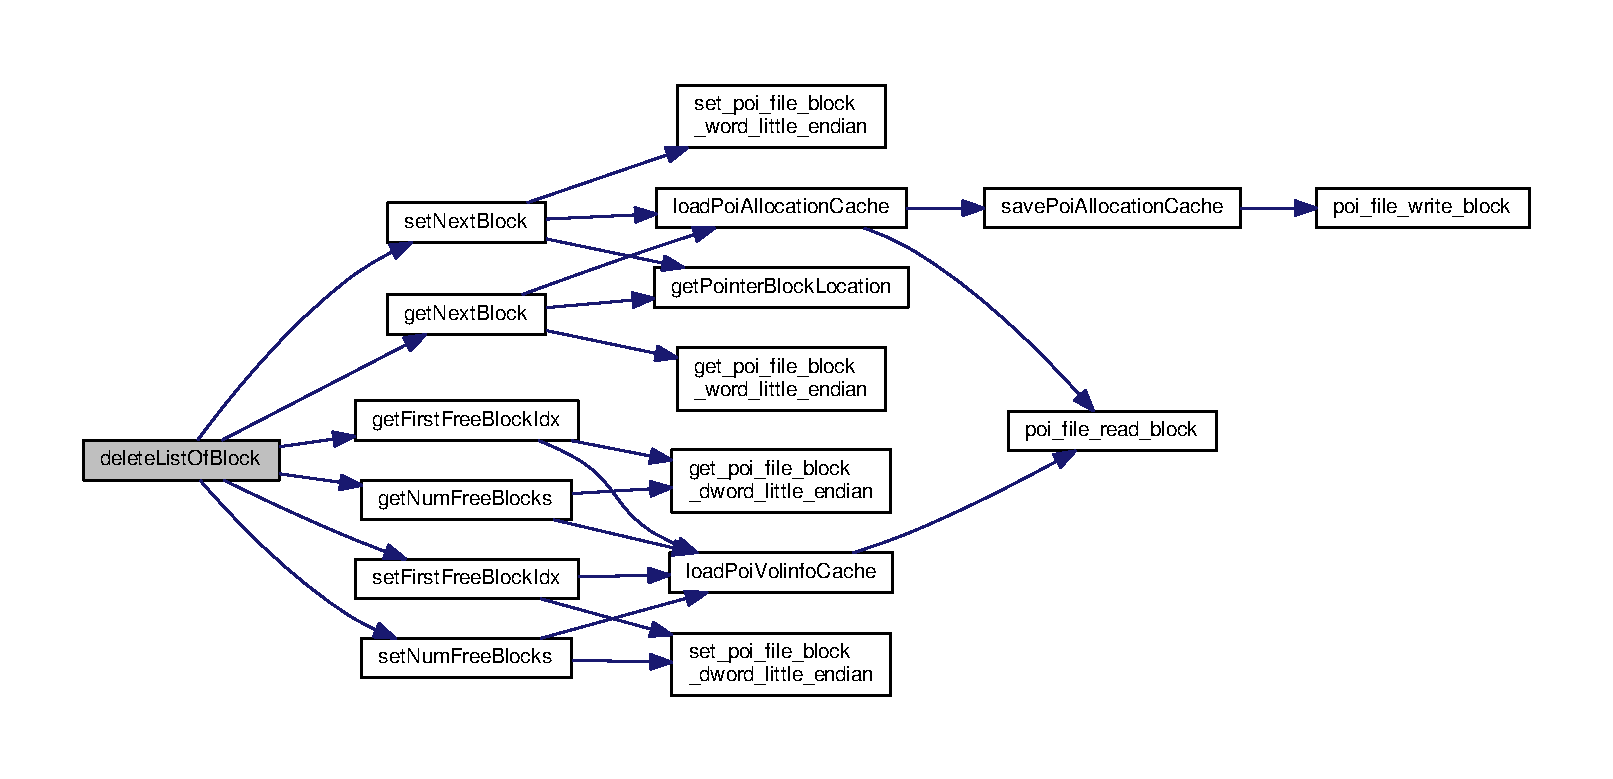
\includegraphics[width=350pt]{allocation-table_8c_a8d703df55ad80bb8fb1177a0542065b6_cgraph}
\end{center}
\end{figure}




Here is the caller graph for this function\-:\nopagebreak
\begin{figure}[H]
\begin{center}
\leavevmode
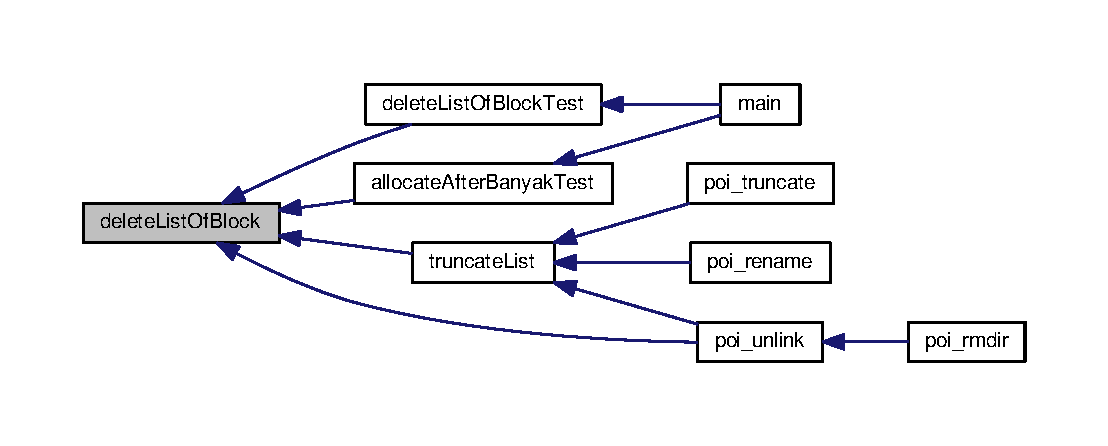
\includegraphics[width=350pt]{allocation-table_8c_a8d703df55ad80bb8fb1177a0542065b6_icgraph}
\end{center}
\end{figure}


\hypertarget{allocation-table_8c_a6de48f9bdf37e8005b9973a75d07633a}{\index{allocation-\/table.\-c@{allocation-\/table.\-c}!insert\-After@{insert\-After}}
\index{insert\-After@{insert\-After}!allocation-table.c@{allocation-\/table.\-c}}
\subsubsection[{insert\-After}]{\setlength{\rightskip}{0pt plus 5cm}int32\-\_\-t insert\-After (
\begin{DoxyParamCaption}
\item[{{\bf poi\-\_\-data\-\_\-pool\-\_\-block\-\_\-idx\-\_\-t}}]{n, }
\item[{{\bf poi\-\_\-file\-\_\-block}}]{blk}
\end{DoxyParamCaption}
)}}\label{allocation-table_8c_a6de48f9bdf37e8005b9973a75d07633a}


Here is the call graph for this function\-:\nopagebreak
\begin{figure}[H]
\begin{center}
\leavevmode
\includegraphics[width=350pt]{allocation-table_8c_a6de48f9bdf37e8005b9973a75d07633a_cgraph}
\end{center}
\end{figure}




Here is the caller graph for this function\-:\nopagebreak
\begin{figure}[H]
\begin{center}
\leavevmode
\includegraphics[width=334pt]{allocation-table_8c_a6de48f9bdf37e8005b9973a75d07633a_icgraph}
\end{center}
\end{figure}


\hypertarget{allocation-table_8c_ada2e09277dd8e97a2b2b75484b738126}{\index{allocation-\/table.\-c@{allocation-\/table.\-c}!new\-List@{new\-List}}
\index{new\-List@{new\-List}!allocation-table.c@{allocation-\/table.\-c}}
\subsubsection[{new\-List}]{\setlength{\rightskip}{0pt plus 5cm}int32\-\_\-t new\-List (
\begin{DoxyParamCaption}
\item[{{\bf poi\-\_\-data\-\_\-pool\-\_\-block\-\_\-idx\-\_\-t} $\ast$}]{n}
\end{DoxyParamCaption}
)}}\label{allocation-table_8c_ada2e09277dd8e97a2b2b75484b738126}


Here is the call graph for this function\-:\nopagebreak
\begin{figure}[H]
\begin{center}
\leavevmode
\includegraphics[width=350pt]{allocation-table_8c_ada2e09277dd8e97a2b2b75484b738126_cgraph}
\end{center}
\end{figure}




Here is the caller graph for this function\-:\nopagebreak
\begin{figure}[H]
\begin{center}
\leavevmode
\includegraphics[width=350pt]{allocation-table_8c_ada2e09277dd8e97a2b2b75484b738126_icgraph}
\end{center}
\end{figure}


\hypertarget{allocation-table_8c_a20af25d3b441d1f25e4830ee2173480c}{\index{allocation-\/table.\-c@{allocation-\/table.\-c}!save\-Alloc\-Table\-Caches@{save\-Alloc\-Table\-Caches}}
\index{save\-Alloc\-Table\-Caches@{save\-Alloc\-Table\-Caches}!allocation-table.c@{allocation-\/table.\-c}}
\subsubsection[{save\-Alloc\-Table\-Caches}]{\setlength{\rightskip}{0pt plus 5cm}void save\-Alloc\-Table\-Caches (
\begin{DoxyParamCaption}
{}
\end{DoxyParamCaption}
)}}\label{allocation-table_8c_a20af25d3b441d1f25e4830ee2173480c}


Here is the call graph for this function\-:\nopagebreak
\begin{figure}[H]
\begin{center}
\leavevmode
\includegraphics[width=350pt]{allocation-table_8c_a20af25d3b441d1f25e4830ee2173480c_cgraph}
\end{center}
\end{figure}




Here is the caller graph for this function\-:\nopagebreak
\begin{figure}[H]
\begin{center}
\leavevmode
\includegraphics[width=350pt]{allocation-table_8c_a20af25d3b441d1f25e4830ee2173480c_icgraph}
\end{center}
\end{figure}


\hypertarget{allocation-table_8c_a986965542b07562f2f205f9d68043a9c}{\index{allocation-\/table.\-c@{allocation-\/table.\-c}!truncate\-List@{truncate\-List}}
\index{truncate\-List@{truncate\-List}!allocation-table.c@{allocation-\/table.\-c}}
\subsubsection[{truncate\-List}]{\setlength{\rightskip}{0pt plus 5cm}void truncate\-List (
\begin{DoxyParamCaption}
\item[{{\bf poi\-\_\-data\-\_\-pool\-\_\-block\-\_\-idx\-\_\-t}}]{n}
\end{DoxyParamCaption}
)}}\label{allocation-table_8c_a986965542b07562f2f205f9d68043a9c}


Here is the call graph for this function\-:\nopagebreak
\begin{figure}[H]
\begin{center}
\leavevmode
\includegraphics[width=350pt]{allocation-table_8c_a986965542b07562f2f205f9d68043a9c_cgraph}
\end{center}
\end{figure}




Here is the caller graph for this function\-:\nopagebreak
\begin{figure}[H]
\begin{center}
\leavevmode
\includegraphics[width=346pt]{allocation-table_8c_a986965542b07562f2f205f9d68043a9c_icgraph}
\end{center}
\end{figure}



\hypertarget{allocation-table_8h}{\section{src/allocation-\/table.h File Reference}
\label{allocation-table_8h}\index{src/allocation-\/table.\-h@{src/allocation-\/table.\-h}}
}
{\ttfamily \#include \char`\"{}allocation-\/block-\/manager.\-h\char`\"{}}\\*
{\ttfamily \#include \char`\"{}volume-\/information.\-h\char`\"{}}\\*
{\ttfamily \#include \char`\"{}data-\/pool-\/block-\/manager.\-h\char`\"{}}\\*
Include dependency graph for allocation-\/table.h\-:
\nopagebreak
\begin{figure}[H]
\begin{center}
\leavevmode
\includegraphics[width=350pt]{allocation-table_8h__incl}
\end{center}
\end{figure}
This graph shows which files directly or indirectly include this file\-:
\nopagebreak
\begin{figure}[H]
\begin{center}
\leavevmode
\includegraphics[width=302pt]{allocation-table_8h__dep__incl}
\end{center}
\end{figure}
\subsection*{Functions}
\begin{DoxyCompactItemize}
\item 
void \hyperlink{allocation-table_8h_a20af25d3b441d1f25e4830ee2173480c}{save\-Alloc\-Table\-Caches} ()
\item 
int32\-\_\-t \hyperlink{allocation-table_8h_ada2e09277dd8e97a2b2b75484b738126}{new\-List} (\hyperlink{data-pool-block-manager_8h_a87e19ab8290bcd76be1c7db1e90cc6f6}{poi\-\_\-data\-\_\-pool\-\_\-block\-\_\-idx\-\_\-t} $\ast$\hyperlink{allocation-table-test_8c_a24010dade8ebab3f87a48022772cd975}{n})
\item 
int32\-\_\-t \hyperlink{allocation-table_8h_a89ea9558bd50decb1bbbf85e569fe6c5}{allocate\-After} (\hyperlink{data-pool-block-manager_8h_a87e19ab8290bcd76be1c7db1e90cc6f6}{poi\-\_\-data\-\_\-pool\-\_\-block\-\_\-idx\-\_\-t} \hyperlink{allocation-table-test_8c_a24010dade8ebab3f87a48022772cd975}{n})
\item 
int32\-\_\-t \hyperlink{allocation-table_8h_a6de48f9bdf37e8005b9973a75d07633a}{insert\-After} (\hyperlink{data-pool-block-manager_8h_a87e19ab8290bcd76be1c7db1e90cc6f6}{poi\-\_\-data\-\_\-pool\-\_\-block\-\_\-idx\-\_\-t} \hyperlink{allocation-table-test_8c_a24010dade8ebab3f87a48022772cd975}{n}, \hyperlink{structpoi__file__block}{poi\-\_\-file\-\_\-block} blk)
\item 
void \hyperlink{allocation-table_8h_a8d703df55ad80bb8fb1177a0542065b6}{delete\-List\-Of\-Block} (\hyperlink{data-pool-block-manager_8h_a87e19ab8290bcd76be1c7db1e90cc6f6}{poi\-\_\-data\-\_\-pool\-\_\-block\-\_\-idx\-\_\-t} \hyperlink{allocation-table-test_8c_a24010dade8ebab3f87a48022772cd975}{n})
\item 
void \hyperlink{allocation-table_8h_a986965542b07562f2f205f9d68043a9c}{truncate\-List} (\hyperlink{data-pool-block-manager_8h_a87e19ab8290bcd76be1c7db1e90cc6f6}{poi\-\_\-data\-\_\-pool\-\_\-block\-\_\-idx\-\_\-t} \hyperlink{allocation-table-test_8c_a24010dade8ebab3f87a48022772cd975}{n})
\end{DoxyCompactItemize}


\subsection{Function Documentation}
\hypertarget{allocation-table_8h_a89ea9558bd50decb1bbbf85e569fe6c5}{\index{allocation-\/table.\-h@{allocation-\/table.\-h}!allocate\-After@{allocate\-After}}
\index{allocate\-After@{allocate\-After}!allocation-table.h@{allocation-\/table.\-h}}
\subsubsection[{allocate\-After}]{\setlength{\rightskip}{0pt plus 5cm}int32\-\_\-t allocate\-After (
\begin{DoxyParamCaption}
\item[{{\bf poi\-\_\-data\-\_\-pool\-\_\-block\-\_\-idx\-\_\-t}}]{n}
\end{DoxyParamCaption}
)}}\label{allocation-table_8h_a89ea9558bd50decb1bbbf85e569fe6c5}


Definition at line 40 of file allocation-\/table.\-c.



Here is the call graph for this function\-:
\nopagebreak
\begin{figure}[H]
\begin{center}
\leavevmode
\includegraphics[width=350pt]{allocation-table_8h_a89ea9558bd50decb1bbbf85e569fe6c5_cgraph}
\end{center}
\end{figure}




Here is the caller graph for this function\-:
\nopagebreak
\begin{figure}[H]
\begin{center}
\leavevmode
\includegraphics[width=350pt]{allocation-table_8h_a89ea9558bd50decb1bbbf85e569fe6c5_icgraph}
\end{center}
\end{figure}


\hypertarget{allocation-table_8h_a8d703df55ad80bb8fb1177a0542065b6}{\index{allocation-\/table.\-h@{allocation-\/table.\-h}!delete\-List\-Of\-Block@{delete\-List\-Of\-Block}}
\index{delete\-List\-Of\-Block@{delete\-List\-Of\-Block}!allocation-table.h@{allocation-\/table.\-h}}
\subsubsection[{delete\-List\-Of\-Block}]{\setlength{\rightskip}{0pt plus 5cm}void delete\-List\-Of\-Block (
\begin{DoxyParamCaption}
\item[{{\bf poi\-\_\-data\-\_\-pool\-\_\-block\-\_\-idx\-\_\-t}}]{n}
\end{DoxyParamCaption}
)}}\label{allocation-table_8h_a8d703df55ad80bb8fb1177a0542065b6}


Definition at line 67 of file allocation-\/table.\-c.



Here is the call graph for this function\-:
\nopagebreak
\begin{figure}[H]
\begin{center}
\leavevmode
\includegraphics[width=350pt]{allocation-table_8h_a8d703df55ad80bb8fb1177a0542065b6_cgraph}
\end{center}
\end{figure}




Here is the caller graph for this function\-:
\nopagebreak
\begin{figure}[H]
\begin{center}
\leavevmode
\includegraphics[width=350pt]{allocation-table_8h_a8d703df55ad80bb8fb1177a0542065b6_icgraph}
\end{center}
\end{figure}


\hypertarget{allocation-table_8h_a6de48f9bdf37e8005b9973a75d07633a}{\index{allocation-\/table.\-h@{allocation-\/table.\-h}!insert\-After@{insert\-After}}
\index{insert\-After@{insert\-After}!allocation-table.h@{allocation-\/table.\-h}}
\subsubsection[{insert\-After}]{\setlength{\rightskip}{0pt plus 5cm}int32\-\_\-t insert\-After (
\begin{DoxyParamCaption}
\item[{{\bf poi\-\_\-data\-\_\-pool\-\_\-block\-\_\-idx\-\_\-t}}]{n, }
\item[{{\bf poi\-\_\-file\-\_\-block}}]{blk}
\end{DoxyParamCaption}
)}}\label{allocation-table_8h_a6de48f9bdf37e8005b9973a75d07633a}


Definition at line 55 of file allocation-\/table.\-c.



Here is the call graph for this function\-:
\nopagebreak
\begin{figure}[H]
\begin{center}
\leavevmode
\includegraphics[width=350pt]{allocation-table_8h_a6de48f9bdf37e8005b9973a75d07633a_cgraph}
\end{center}
\end{figure}




Here is the caller graph for this function\-:
\nopagebreak
\begin{figure}[H]
\begin{center}
\leavevmode
\includegraphics[width=334pt]{allocation-table_8h_a6de48f9bdf37e8005b9973a75d07633a_icgraph}
\end{center}
\end{figure}


\hypertarget{allocation-table_8h_ada2e09277dd8e97a2b2b75484b738126}{\index{allocation-\/table.\-h@{allocation-\/table.\-h}!new\-List@{new\-List}}
\index{new\-List@{new\-List}!allocation-table.h@{allocation-\/table.\-h}}
\subsubsection[{new\-List}]{\setlength{\rightskip}{0pt plus 5cm}int32\-\_\-t new\-List (
\begin{DoxyParamCaption}
\item[{{\bf poi\-\_\-data\-\_\-pool\-\_\-block\-\_\-idx\-\_\-t} $\ast$}]{n}
\end{DoxyParamCaption}
)}}\label{allocation-table_8h_ada2e09277dd8e97a2b2b75484b738126}


Definition at line 25 of file allocation-\/table.\-c.



Here is the call graph for this function\-:
\nopagebreak
\begin{figure}[H]
\begin{center}
\leavevmode
\includegraphics[width=350pt]{allocation-table_8h_ada2e09277dd8e97a2b2b75484b738126_cgraph}
\end{center}
\end{figure}




Here is the caller graph for this function\-:
\nopagebreak
\begin{figure}[H]
\begin{center}
\leavevmode
\includegraphics[width=350pt]{allocation-table_8h_ada2e09277dd8e97a2b2b75484b738126_icgraph}
\end{center}
\end{figure}


\hypertarget{allocation-table_8h_a20af25d3b441d1f25e4830ee2173480c}{\index{allocation-\/table.\-h@{allocation-\/table.\-h}!save\-Alloc\-Table\-Caches@{save\-Alloc\-Table\-Caches}}
\index{save\-Alloc\-Table\-Caches@{save\-Alloc\-Table\-Caches}!allocation-table.h@{allocation-\/table.\-h}}
\subsubsection[{save\-Alloc\-Table\-Caches}]{\setlength{\rightskip}{0pt plus 5cm}void save\-Alloc\-Table\-Caches (
\begin{DoxyParamCaption}
{}
\end{DoxyParamCaption}
)}}\label{allocation-table_8h_a20af25d3b441d1f25e4830ee2173480c}


Definition at line 14 of file allocation-\/table.\-c.



Here is the call graph for this function\-:
\nopagebreak
\begin{figure}[H]
\begin{center}
\leavevmode
\includegraphics[width=350pt]{allocation-table_8h_a20af25d3b441d1f25e4830ee2173480c_cgraph}
\end{center}
\end{figure}


\hypertarget{allocation-table_8h_a986965542b07562f2f205f9d68043a9c}{\index{allocation-\/table.\-h@{allocation-\/table.\-h}!truncate\-List@{truncate\-List}}
\index{truncate\-List@{truncate\-List}!allocation-table.h@{allocation-\/table.\-h}}
\subsubsection[{truncate\-List}]{\setlength{\rightskip}{0pt plus 5cm}void truncate\-List (
\begin{DoxyParamCaption}
\item[{{\bf poi\-\_\-data\-\_\-pool\-\_\-block\-\_\-idx\-\_\-t}}]{n}
\end{DoxyParamCaption}
)}}\label{allocation-table_8h_a986965542b07562f2f205f9d68043a9c}


Definition at line 91 of file allocation-\/table.\-c.



Here is the call graph for this function\-:
\nopagebreak
\begin{figure}[H]
\begin{center}
\leavevmode
\includegraphics[width=350pt]{allocation-table_8h_a986965542b07562f2f205f9d68043a9c_cgraph}
\end{center}
\end{figure}




Here is the caller graph for this function\-:
\nopagebreak
\begin{figure}[H]
\begin{center}
\leavevmode
\includegraphics[width=346pt]{allocation-table_8h_a986965542b07562f2f205f9d68043a9c_icgraph}
\end{center}
\end{figure}



\hypertarget{data-pool-block-manager-test_8c}{\section{src/data-\/pool-\/block-\/manager-\/test.c File Reference}
\label{data-pool-block-manager-test_8c}\index{src/data-\/pool-\/block-\/manager-\/test.\-c@{src/data-\/pool-\/block-\/manager-\/test.\-c}}
}
{\ttfamily \#include \char`\"{}data-\/pool-\/block-\/manager.\-h\char`\"{}}\\*
{\ttfamily \#include $<$assert.\-h$>$}\\*
Include dependency graph for data-\/pool-\/block-\/manager-\/test.c\-:
\nopagebreak
\begin{figure}[H]
\begin{center}
\leavevmode
\includegraphics[width=305pt]{data-pool-block-manager-test_8c__incl}
\end{center}
\end{figure}
\subsection*{Functions}
\begin{DoxyCompactItemize}
\item 
void \hyperlink{data-pool-block-manager-test_8c_ae85954364eb34c20aec506171ba5f351}{test\-Constants} ()
\item 
void \hyperlink{data-pool-block-manager-test_8c_a75323f97b259a6284370855087fb48ff}{test\-Read\-Write} ()
\item 
int \hyperlink{data-pool-block-manager-test_8c_ae66f6b31b5ad750f1fe042a706a4e3d4}{main} ()
\end{DoxyCompactItemize}


\subsection{Function Documentation}
\hypertarget{data-pool-block-manager-test_8c_ae66f6b31b5ad750f1fe042a706a4e3d4}{\index{data-\/pool-\/block-\/manager-\/test.\-c@{data-\/pool-\/block-\/manager-\/test.\-c}!main@{main}}
\index{main@{main}!data-pool-block-manager-test.c@{data-\/pool-\/block-\/manager-\/test.\-c}}
\subsubsection[{main}]{\setlength{\rightskip}{0pt plus 5cm}int main (
\begin{DoxyParamCaption}
{}
\end{DoxyParamCaption}
)}}\label{data-pool-block-manager-test_8c_ae66f6b31b5ad750f1fe042a706a4e3d4}


Definition at line 23 of file data-\/pool-\/block-\/manager-\/test.\-c.



Here is the call graph for this function\-:
\nopagebreak
\begin{figure}[H]
\begin{center}
\leavevmode
\includegraphics[width=350pt]{data-pool-block-manager-test_8c_ae66f6b31b5ad750f1fe042a706a4e3d4_cgraph}
\end{center}
\end{figure}


\hypertarget{data-pool-block-manager-test_8c_ae85954364eb34c20aec506171ba5f351}{\index{data-\/pool-\/block-\/manager-\/test.\-c@{data-\/pool-\/block-\/manager-\/test.\-c}!test\-Constants@{test\-Constants}}
\index{test\-Constants@{test\-Constants}!data-pool-block-manager-test.c@{data-\/pool-\/block-\/manager-\/test.\-c}}
\subsubsection[{test\-Constants}]{\setlength{\rightskip}{0pt plus 5cm}void test\-Constants (
\begin{DoxyParamCaption}
{}
\end{DoxyParamCaption}
)}}\label{data-pool-block-manager-test_8c_ae85954364eb34c20aec506171ba5f351}


Definition at line 4 of file data-\/pool-\/block-\/manager-\/test.\-c.



Here is the caller graph for this function\-:
\nopagebreak
\begin{figure}[H]
\begin{center}
\leavevmode
\includegraphics[width=232pt]{data-pool-block-manager-test_8c_ae85954364eb34c20aec506171ba5f351_icgraph}
\end{center}
\end{figure}


\hypertarget{data-pool-block-manager-test_8c_a75323f97b259a6284370855087fb48ff}{\index{data-\/pool-\/block-\/manager-\/test.\-c@{data-\/pool-\/block-\/manager-\/test.\-c}!test\-Read\-Write@{test\-Read\-Write}}
\index{test\-Read\-Write@{test\-Read\-Write}!data-pool-block-manager-test.c@{data-\/pool-\/block-\/manager-\/test.\-c}}
\subsubsection[{test\-Read\-Write}]{\setlength{\rightskip}{0pt plus 5cm}void test\-Read\-Write (
\begin{DoxyParamCaption}
{}
\end{DoxyParamCaption}
)}}\label{data-pool-block-manager-test_8c_a75323f97b259a6284370855087fb48ff}


Definition at line 9 of file data-\/pool-\/block-\/manager-\/test.\-c.



Here is the call graph for this function\-:
\nopagebreak
\begin{figure}[H]
\begin{center}
\leavevmode
\includegraphics[width=350pt]{data-pool-block-manager-test_8c_a75323f97b259a6284370855087fb48ff_cgraph}
\end{center}
\end{figure}




Here is the caller graph for this function\-:
\nopagebreak
\begin{figure}[H]
\begin{center}
\leavevmode
\includegraphics[width=234pt]{data-pool-block-manager-test_8c_a75323f97b259a6284370855087fb48ff_icgraph}
\end{center}
\end{figure}



\hypertarget{data-pool-block-manager_8c}{\section{src/data-\/pool-\/block-\/manager.c File Reference}
\label{data-pool-block-manager_8c}\index{src/data-\/pool-\/block-\/manager.\-c@{src/data-\/pool-\/block-\/manager.\-c}}
}
{\ttfamily \#include \char`\"{}file-\/manager.\-h\char`\"{}}\\*
{\ttfamily \#include \char`\"{}data-\/pool-\/block-\/manager.\-h\char`\"{}}\\*
{\ttfamily \#include $<$assert.\-h$>$}\\*
Include dependency graph for data-\/pool-\/block-\/manager.c\-:
\nopagebreak
\begin{figure}[H]
\begin{center}
\leavevmode
\includegraphics[width=350pt]{data-pool-block-manager_8c__incl}
\end{center}
\end{figure}
\subsection*{Macros}
\begin{DoxyCompactItemize}
\item 
\#define \hyperlink{data-pool-block-manager_8c_acc334690346a1892e11c892ed27f70e7}{data\-\_\-pool\-\_\-block\-\_\-manager\-\_\-c}
\end{DoxyCompactItemize}
\subsection*{Functions}
\begin{DoxyCompactItemize}
\item 
\hyperlink{structpoi__file__block}{poi\-\_\-file\-\_\-block} \hyperlink{data-pool-block-manager_8c_ac930ae4a4b3ca65a49d45c7654f15149}{poi\-\_\-data\-\_\-pool\-\_\-read\-\_\-block} (\hyperlink{data-pool-block-manager_8h_a87e19ab8290bcd76be1c7db1e90cc6f6}{poi\-\_\-data\-\_\-pool\-\_\-block\-\_\-idx\-\_\-t} \hyperlink{allocation-table-test_8c_a24010dade8ebab3f87a48022772cd975}{n})
\item 
int \hyperlink{data-pool-block-manager_8c_a10624f1cbc61dd0a8a03aa94d8502567}{poi\-\_\-data\-\_\-pool\-\_\-write\-\_\-block} (\hyperlink{structpoi__file__block}{poi\-\_\-file\-\_\-block} b, \hyperlink{data-pool-block-manager_8h_a87e19ab8290bcd76be1c7db1e90cc6f6}{poi\-\_\-data\-\_\-pool\-\_\-block\-\_\-idx\-\_\-t} \hyperlink{allocation-table-test_8c_a24010dade8ebab3f87a48022772cd975}{n})
\end{DoxyCompactItemize}


\subsection{Macro Definition Documentation}
\hypertarget{data-pool-block-manager_8c_acc334690346a1892e11c892ed27f70e7}{\index{data-\/pool-\/block-\/manager.\-c@{data-\/pool-\/block-\/manager.\-c}!data\-\_\-pool\-\_\-block\-\_\-manager\-\_\-c@{data\-\_\-pool\-\_\-block\-\_\-manager\-\_\-c}}
\index{data\-\_\-pool\-\_\-block\-\_\-manager\-\_\-c@{data\-\_\-pool\-\_\-block\-\_\-manager\-\_\-c}!data-pool-block-manager.c@{data-\/pool-\/block-\/manager.\-c}}
\subsubsection[{data\-\_\-pool\-\_\-block\-\_\-manager\-\_\-c}]{\setlength{\rightskip}{0pt plus 5cm}\#define data\-\_\-pool\-\_\-block\-\_\-manager\-\_\-c}}\label{data-pool-block-manager_8c_acc334690346a1892e11c892ed27f70e7}


Definition at line 2 of file data-\/pool-\/block-\/manager.\-c.



\subsection{Function Documentation}
\hypertarget{data-pool-block-manager_8c_ac930ae4a4b3ca65a49d45c7654f15149}{\index{data-\/pool-\/block-\/manager.\-c@{data-\/pool-\/block-\/manager.\-c}!poi\-\_\-data\-\_\-pool\-\_\-read\-\_\-block@{poi\-\_\-data\-\_\-pool\-\_\-read\-\_\-block}}
\index{poi\-\_\-data\-\_\-pool\-\_\-read\-\_\-block@{poi\-\_\-data\-\_\-pool\-\_\-read\-\_\-block}!data-pool-block-manager.c@{data-\/pool-\/block-\/manager.\-c}}
\subsubsection[{poi\-\_\-data\-\_\-pool\-\_\-read\-\_\-block}]{\setlength{\rightskip}{0pt plus 5cm}{\bf poi\-\_\-file\-\_\-block} poi\-\_\-data\-\_\-pool\-\_\-read\-\_\-block (
\begin{DoxyParamCaption}
\item[{{\bf poi\-\_\-data\-\_\-pool\-\_\-block\-\_\-idx\-\_\-t}}]{n}
\end{DoxyParamCaption}
)}}\label{data-pool-block-manager_8c_ac930ae4a4b3ca65a49d45c7654f15149}


Definition at line 10 of file data-\/pool-\/block-\/manager.\-c.



Here is the call graph for this function\-:
\nopagebreak
\begin{figure}[H]
\begin{center}
\leavevmode
\includegraphics[width=318pt]{data-pool-block-manager_8c_ac930ae4a4b3ca65a49d45c7654f15149_cgraph}
\end{center}
\end{figure}




Here is the caller graph for this function\-:
\nopagebreak
\begin{figure}[H]
\begin{center}
\leavevmode
\includegraphics[width=350pt]{data-pool-block-manager_8c_ac930ae4a4b3ca65a49d45c7654f15149_icgraph}
\end{center}
\end{figure}


\hypertarget{data-pool-block-manager_8c_a10624f1cbc61dd0a8a03aa94d8502567}{\index{data-\/pool-\/block-\/manager.\-c@{data-\/pool-\/block-\/manager.\-c}!poi\-\_\-data\-\_\-pool\-\_\-write\-\_\-block@{poi\-\_\-data\-\_\-pool\-\_\-write\-\_\-block}}
\index{poi\-\_\-data\-\_\-pool\-\_\-write\-\_\-block@{poi\-\_\-data\-\_\-pool\-\_\-write\-\_\-block}!data-pool-block-manager.c@{data-\/pool-\/block-\/manager.\-c}}
\subsubsection[{poi\-\_\-data\-\_\-pool\-\_\-write\-\_\-block}]{\setlength{\rightskip}{0pt plus 5cm}int poi\-\_\-data\-\_\-pool\-\_\-write\-\_\-block (
\begin{DoxyParamCaption}
\item[{{\bf poi\-\_\-file\-\_\-block}}]{b, }
\item[{{\bf poi\-\_\-data\-\_\-pool\-\_\-block\-\_\-idx\-\_\-t}}]{n}
\end{DoxyParamCaption}
)}}\label{data-pool-block-manager_8c_a10624f1cbc61dd0a8a03aa94d8502567}


Definition at line 17 of file data-\/pool-\/block-\/manager.\-c.



Here is the call graph for this function\-:
\nopagebreak
\begin{figure}[H]
\begin{center}
\leavevmode
\includegraphics[width=322pt]{data-pool-block-manager_8c_a10624f1cbc61dd0a8a03aa94d8502567_cgraph}
\end{center}
\end{figure}




Here is the caller graph for this function\-:
\nopagebreak
\begin{figure}[H]
\begin{center}
\leavevmode
\includegraphics[width=350pt]{data-pool-block-manager_8c_a10624f1cbc61dd0a8a03aa94d8502567_icgraph}
\end{center}
\end{figure}



\hypertarget{data-pool-block-manager_8h}{\section{src/data-\/pool-\/block-\/manager.h File Reference}
\label{data-pool-block-manager_8h}\index{src/data-\/pool-\/block-\/manager.\-h@{src/data-\/pool-\/block-\/manager.\-h}}
}


mengatur pembacaan dan penulisan blok kantong data  


{\ttfamily \#include \char`\"{}file-\/manager.\-h\char`\"{}}\\*
Include dependency graph for data-\/pool-\/block-\/manager.h\-:\nopagebreak
\begin{figure}[H]
\begin{center}
\leavevmode
\includegraphics[width=258pt]{data-pool-block-manager_8h__incl}
\end{center}
\end{figure}
This graph shows which files directly or indirectly include this file\-:\nopagebreak
\begin{figure}[H]
\begin{center}
\leavevmode
\includegraphics[width=350pt]{data-pool-block-manager_8h__dep__incl}
\end{center}
\end{figure}
\subsection*{Macros}
\begin{DoxyCompactItemize}
\item 
\#define \hyperlink{data-pool-block-manager_8h_ab249bb14ed04381809b0cfeffaa6e01d}{D\-A\-T\-A\-\_\-\-P\-O\-O\-L\-\_\-\-B\-L\-O\-C\-K\-\_\-\-M\-I\-N\-\_\-\-I\-D\-X}~0
\item 
\#define \hyperlink{data-pool-block-manager_8h_a7d56b75785e6fcf7a7e48cf1e0597fce}{D\-A\-T\-A\-\_\-\-P\-O\-O\-L\-\_\-\-B\-L\-O\-C\-K\-\_\-\-M\-A\-X\-\_\-\-I\-D\-X}~(\hyperlink{file-manager_8h_a6e4b52d19d492676f83a8576aba19a34}{P\-O\-I\-\_\-\-D\-A\-T\-A\-\_\-\-P\-O\-O\-L\-\_\-\-B\-L\-O\-C\-K\-S\-\_\-\-N\-U\-M}-\/1)
\item 
\#define \hyperlink{data-pool-block-manager_8h_ae9bd339a611ae2c33781964f7337dff5}{D\-A\-T\-A\-\_\-\-P\-O\-O\-L\-\_\-\-B\-L\-O\-C\-K\-\_\-\-M\-I\-N\-\_\-\-N\-U\-M}~(\hyperlink{file-manager_8h_a87ede160157563bbccc56097d4c431d7}{P\-O\-I\-\_\-\-V\-O\-L\-U\-M\-E\-\_\-\-I\-N\-F\-O\-R\-M\-A\-T\-I\-O\-N\-\_\-\-B\-L\-O\-C\-K\-S\-\_\-\-N\-U\-M} + \hyperlink{file-manager_8h_a555a4a22088989bb446cc085f19844ec}{P\-O\-I\-\_\-\-A\-L\-L\-O\-C\-A\-T\-I\-O\-N\-\_\-\-T\-A\-B\-L\-E\-\_\-\-B\-L\-O\-C\-K\-S\-\_\-\-N\-U\-M})
\item 
\#define \hyperlink{data-pool-block-manager_8h_a7154b2941bf1144d8886fdbafc64a1ff}{D\-A\-T\-A\-\_\-\-P\-O\-O\-L\-\_\-\-B\-L\-O\-C\-K\-\_\-\-M\-A\-X\-\_\-\-N\-U\-M}~(\hyperlink{data-pool-block-manager_8h_ae9bd339a611ae2c33781964f7337dff5}{D\-A\-T\-A\-\_\-\-P\-O\-O\-L\-\_\-\-B\-L\-O\-C\-K\-\_\-\-M\-I\-N\-\_\-\-N\-U\-M}+\hyperlink{data-pool-block-manager_8h_a7d56b75785e6fcf7a7e48cf1e0597fce}{D\-A\-T\-A\-\_\-\-P\-O\-O\-L\-\_\-\-B\-L\-O\-C\-K\-\_\-\-M\-A\-X\-\_\-\-I\-D\-X})
\end{DoxyCompactItemize}
\subsection*{Typedefs}
\begin{DoxyCompactItemize}
\item 
typedef uint16\-\_\-t \hyperlink{data-pool-block-manager_8h_a87e19ab8290bcd76be1c7db1e90cc6f6}{poi\-\_\-data\-\_\-pool\-\_\-block\-\_\-idx\-\_\-t}
\end{DoxyCompactItemize}
\subsection*{Functions}
\begin{DoxyCompactItemize}
\item 
\hyperlink{structpoi__file__block}{poi\-\_\-file\-\_\-block} \hyperlink{data-pool-block-manager_8h_ac930ae4a4b3ca65a49d45c7654f15149}{poi\-\_\-data\-\_\-pool\-\_\-read\-\_\-block} (\hyperlink{data-pool-block-manager_8h_a87e19ab8290bcd76be1c7db1e90cc6f6}{poi\-\_\-data\-\_\-pool\-\_\-block\-\_\-idx\-\_\-t} \hyperlink{allocation-table-test_8c_a24010dade8ebab3f87a48022772cd975}{n})
\item 
int \hyperlink{data-pool-block-manager_8h_a10624f1cbc61dd0a8a03aa94d8502567}{poi\-\_\-data\-\_\-pool\-\_\-write\-\_\-block} (\hyperlink{structpoi__file__block}{poi\-\_\-file\-\_\-block} b, \hyperlink{data-pool-block-manager_8h_a87e19ab8290bcd76be1c7db1e90cc6f6}{poi\-\_\-data\-\_\-pool\-\_\-block\-\_\-idx\-\_\-t} \hyperlink{allocation-table-test_8c_a24010dade8ebab3f87a48022772cd975}{n})
\item 
\hyperlink{data-pool-block-manager_8h_a87e19ab8290bcd76be1c7db1e90cc6f6}{poi\-\_\-data\-\_\-pool\-\_\-block\-\_\-idx\-\_\-t} \hyperlink{data-pool-block-manager_8h_ae02f040d4e0f458f0d63751bc09f55b7}{poi\-\_\-data\-\_\-pool\-\_\-get\-\_\-next\-\_\-empty} (\hyperlink{data-pool-block-manager_8h_a87e19ab8290bcd76be1c7db1e90cc6f6}{poi\-\_\-data\-\_\-pool\-\_\-block\-\_\-idx\-\_\-t} \hyperlink{allocation-table-test_8c_a24010dade8ebab3f87a48022772cd975}{n})
\end{DoxyCompactItemize}


\subsection{Detailed Description}
mengatur pembacaan dan penulisan blok kantong data \begin{DoxyAuthor}{Author}
jang berikoetnja 
\end{DoxyAuthor}


\subsection{Macro Definition Documentation}
\hypertarget{data-pool-block-manager_8h_a7d56b75785e6fcf7a7e48cf1e0597fce}{\index{data-\/pool-\/block-\/manager.\-h@{data-\/pool-\/block-\/manager.\-h}!D\-A\-T\-A\-\_\-\-P\-O\-O\-L\-\_\-\-B\-L\-O\-C\-K\-\_\-\-M\-A\-X\-\_\-\-I\-D\-X@{D\-A\-T\-A\-\_\-\-P\-O\-O\-L\-\_\-\-B\-L\-O\-C\-K\-\_\-\-M\-A\-X\-\_\-\-I\-D\-X}}
\index{D\-A\-T\-A\-\_\-\-P\-O\-O\-L\-\_\-\-B\-L\-O\-C\-K\-\_\-\-M\-A\-X\-\_\-\-I\-D\-X@{D\-A\-T\-A\-\_\-\-P\-O\-O\-L\-\_\-\-B\-L\-O\-C\-K\-\_\-\-M\-A\-X\-\_\-\-I\-D\-X}!data-pool-block-manager.h@{data-\/pool-\/block-\/manager.\-h}}
\subsubsection[{D\-A\-T\-A\-\_\-\-P\-O\-O\-L\-\_\-\-B\-L\-O\-C\-K\-\_\-\-M\-A\-X\-\_\-\-I\-D\-X}]{\setlength{\rightskip}{0pt plus 5cm}\#define D\-A\-T\-A\-\_\-\-P\-O\-O\-L\-\_\-\-B\-L\-O\-C\-K\-\_\-\-M\-A\-X\-\_\-\-I\-D\-X~({\bf P\-O\-I\-\_\-\-D\-A\-T\-A\-\_\-\-P\-O\-O\-L\-\_\-\-B\-L\-O\-C\-K\-S\-\_\-\-N\-U\-M}-\/1)}}\label{data-pool-block-manager_8h_a7d56b75785e6fcf7a7e48cf1e0597fce}
\hypertarget{data-pool-block-manager_8h_a7154b2941bf1144d8886fdbafc64a1ff}{\index{data-\/pool-\/block-\/manager.\-h@{data-\/pool-\/block-\/manager.\-h}!D\-A\-T\-A\-\_\-\-P\-O\-O\-L\-\_\-\-B\-L\-O\-C\-K\-\_\-\-M\-A\-X\-\_\-\-N\-U\-M@{D\-A\-T\-A\-\_\-\-P\-O\-O\-L\-\_\-\-B\-L\-O\-C\-K\-\_\-\-M\-A\-X\-\_\-\-N\-U\-M}}
\index{D\-A\-T\-A\-\_\-\-P\-O\-O\-L\-\_\-\-B\-L\-O\-C\-K\-\_\-\-M\-A\-X\-\_\-\-N\-U\-M@{D\-A\-T\-A\-\_\-\-P\-O\-O\-L\-\_\-\-B\-L\-O\-C\-K\-\_\-\-M\-A\-X\-\_\-\-N\-U\-M}!data-pool-block-manager.h@{data-\/pool-\/block-\/manager.\-h}}
\subsubsection[{D\-A\-T\-A\-\_\-\-P\-O\-O\-L\-\_\-\-B\-L\-O\-C\-K\-\_\-\-M\-A\-X\-\_\-\-N\-U\-M}]{\setlength{\rightskip}{0pt plus 5cm}\#define D\-A\-T\-A\-\_\-\-P\-O\-O\-L\-\_\-\-B\-L\-O\-C\-K\-\_\-\-M\-A\-X\-\_\-\-N\-U\-M~({\bf D\-A\-T\-A\-\_\-\-P\-O\-O\-L\-\_\-\-B\-L\-O\-C\-K\-\_\-\-M\-I\-N\-\_\-\-N\-U\-M}+{\bf D\-A\-T\-A\-\_\-\-P\-O\-O\-L\-\_\-\-B\-L\-O\-C\-K\-\_\-\-M\-A\-X\-\_\-\-I\-D\-X})}}\label{data-pool-block-manager_8h_a7154b2941bf1144d8886fdbafc64a1ff}
\hypertarget{data-pool-block-manager_8h_ab249bb14ed04381809b0cfeffaa6e01d}{\index{data-\/pool-\/block-\/manager.\-h@{data-\/pool-\/block-\/manager.\-h}!D\-A\-T\-A\-\_\-\-P\-O\-O\-L\-\_\-\-B\-L\-O\-C\-K\-\_\-\-M\-I\-N\-\_\-\-I\-D\-X@{D\-A\-T\-A\-\_\-\-P\-O\-O\-L\-\_\-\-B\-L\-O\-C\-K\-\_\-\-M\-I\-N\-\_\-\-I\-D\-X}}
\index{D\-A\-T\-A\-\_\-\-P\-O\-O\-L\-\_\-\-B\-L\-O\-C\-K\-\_\-\-M\-I\-N\-\_\-\-I\-D\-X@{D\-A\-T\-A\-\_\-\-P\-O\-O\-L\-\_\-\-B\-L\-O\-C\-K\-\_\-\-M\-I\-N\-\_\-\-I\-D\-X}!data-pool-block-manager.h@{data-\/pool-\/block-\/manager.\-h}}
\subsubsection[{D\-A\-T\-A\-\_\-\-P\-O\-O\-L\-\_\-\-B\-L\-O\-C\-K\-\_\-\-M\-I\-N\-\_\-\-I\-D\-X}]{\setlength{\rightskip}{0pt plus 5cm}\#define D\-A\-T\-A\-\_\-\-P\-O\-O\-L\-\_\-\-B\-L\-O\-C\-K\-\_\-\-M\-I\-N\-\_\-\-I\-D\-X~0}}\label{data-pool-block-manager_8h_ab249bb14ed04381809b0cfeffaa6e01d}
\hypertarget{data-pool-block-manager_8h_ae9bd339a611ae2c33781964f7337dff5}{\index{data-\/pool-\/block-\/manager.\-h@{data-\/pool-\/block-\/manager.\-h}!D\-A\-T\-A\-\_\-\-P\-O\-O\-L\-\_\-\-B\-L\-O\-C\-K\-\_\-\-M\-I\-N\-\_\-\-N\-U\-M@{D\-A\-T\-A\-\_\-\-P\-O\-O\-L\-\_\-\-B\-L\-O\-C\-K\-\_\-\-M\-I\-N\-\_\-\-N\-U\-M}}
\index{D\-A\-T\-A\-\_\-\-P\-O\-O\-L\-\_\-\-B\-L\-O\-C\-K\-\_\-\-M\-I\-N\-\_\-\-N\-U\-M@{D\-A\-T\-A\-\_\-\-P\-O\-O\-L\-\_\-\-B\-L\-O\-C\-K\-\_\-\-M\-I\-N\-\_\-\-N\-U\-M}!data-pool-block-manager.h@{data-\/pool-\/block-\/manager.\-h}}
\subsubsection[{D\-A\-T\-A\-\_\-\-P\-O\-O\-L\-\_\-\-B\-L\-O\-C\-K\-\_\-\-M\-I\-N\-\_\-\-N\-U\-M}]{\setlength{\rightskip}{0pt plus 5cm}\#define D\-A\-T\-A\-\_\-\-P\-O\-O\-L\-\_\-\-B\-L\-O\-C\-K\-\_\-\-M\-I\-N\-\_\-\-N\-U\-M~({\bf P\-O\-I\-\_\-\-V\-O\-L\-U\-M\-E\-\_\-\-I\-N\-F\-O\-R\-M\-A\-T\-I\-O\-N\-\_\-\-B\-L\-O\-C\-K\-S\-\_\-\-N\-U\-M} + {\bf P\-O\-I\-\_\-\-A\-L\-L\-O\-C\-A\-T\-I\-O\-N\-\_\-\-T\-A\-B\-L\-E\-\_\-\-B\-L\-O\-C\-K\-S\-\_\-\-N\-U\-M})}}\label{data-pool-block-manager_8h_ae9bd339a611ae2c33781964f7337dff5}


\subsection{Typedef Documentation}
\hypertarget{data-pool-block-manager_8h_a87e19ab8290bcd76be1c7db1e90cc6f6}{\index{data-\/pool-\/block-\/manager.\-h@{data-\/pool-\/block-\/manager.\-h}!poi\-\_\-data\-\_\-pool\-\_\-block\-\_\-idx\-\_\-t@{poi\-\_\-data\-\_\-pool\-\_\-block\-\_\-idx\-\_\-t}}
\index{poi\-\_\-data\-\_\-pool\-\_\-block\-\_\-idx\-\_\-t@{poi\-\_\-data\-\_\-pool\-\_\-block\-\_\-idx\-\_\-t}!data-pool-block-manager.h@{data-\/pool-\/block-\/manager.\-h}}
\subsubsection[{poi\-\_\-data\-\_\-pool\-\_\-block\-\_\-idx\-\_\-t}]{\setlength{\rightskip}{0pt plus 5cm}typedef uint16\-\_\-t {\bf poi\-\_\-data\-\_\-pool\-\_\-block\-\_\-idx\-\_\-t}}}\label{data-pool-block-manager_8h_a87e19ab8290bcd76be1c7db1e90cc6f6}


\subsection{Function Documentation}
\hypertarget{data-pool-block-manager_8h_ae02f040d4e0f458f0d63751bc09f55b7}{\index{data-\/pool-\/block-\/manager.\-h@{data-\/pool-\/block-\/manager.\-h}!poi\-\_\-data\-\_\-pool\-\_\-get\-\_\-next\-\_\-empty@{poi\-\_\-data\-\_\-pool\-\_\-get\-\_\-next\-\_\-empty}}
\index{poi\-\_\-data\-\_\-pool\-\_\-get\-\_\-next\-\_\-empty@{poi\-\_\-data\-\_\-pool\-\_\-get\-\_\-next\-\_\-empty}!data-pool-block-manager.h@{data-\/pool-\/block-\/manager.\-h}}
\subsubsection[{poi\-\_\-data\-\_\-pool\-\_\-get\-\_\-next\-\_\-empty}]{\setlength{\rightskip}{0pt plus 5cm}{\bf poi\-\_\-data\-\_\-pool\-\_\-block\-\_\-idx\-\_\-t} poi\-\_\-data\-\_\-pool\-\_\-get\-\_\-next\-\_\-empty (
\begin{DoxyParamCaption}
\item[{{\bf poi\-\_\-data\-\_\-pool\-\_\-block\-\_\-idx\-\_\-t}}]{n}
\end{DoxyParamCaption}
)}}\label{data-pool-block-manager_8h_ae02f040d4e0f458f0d63751bc09f55b7}
\hypertarget{data-pool-block-manager_8h_ac930ae4a4b3ca65a49d45c7654f15149}{\index{data-\/pool-\/block-\/manager.\-h@{data-\/pool-\/block-\/manager.\-h}!poi\-\_\-data\-\_\-pool\-\_\-read\-\_\-block@{poi\-\_\-data\-\_\-pool\-\_\-read\-\_\-block}}
\index{poi\-\_\-data\-\_\-pool\-\_\-read\-\_\-block@{poi\-\_\-data\-\_\-pool\-\_\-read\-\_\-block}!data-pool-block-manager.h@{data-\/pool-\/block-\/manager.\-h}}
\subsubsection[{poi\-\_\-data\-\_\-pool\-\_\-read\-\_\-block}]{\setlength{\rightskip}{0pt plus 5cm}{\bf poi\-\_\-file\-\_\-block} poi\-\_\-data\-\_\-pool\-\_\-read\-\_\-block (
\begin{DoxyParamCaption}
\item[{{\bf poi\-\_\-data\-\_\-pool\-\_\-block\-\_\-idx\-\_\-t}}]{n}
\end{DoxyParamCaption}
)}}\label{data-pool-block-manager_8h_ac930ae4a4b3ca65a49d45c7654f15149}


Here is the call graph for this function\-:\nopagebreak
\begin{figure}[H]
\begin{center}
\leavevmode
\includegraphics[width=318pt]{data-pool-block-manager_8h_ac930ae4a4b3ca65a49d45c7654f15149_cgraph}
\end{center}
\end{figure}




Here is the caller graph for this function\-:\nopagebreak
\begin{figure}[H]
\begin{center}
\leavevmode
\includegraphics[width=350pt]{data-pool-block-manager_8h_ac930ae4a4b3ca65a49d45c7654f15149_icgraph}
\end{center}
\end{figure}


\hypertarget{data-pool-block-manager_8h_a10624f1cbc61dd0a8a03aa94d8502567}{\index{data-\/pool-\/block-\/manager.\-h@{data-\/pool-\/block-\/manager.\-h}!poi\-\_\-data\-\_\-pool\-\_\-write\-\_\-block@{poi\-\_\-data\-\_\-pool\-\_\-write\-\_\-block}}
\index{poi\-\_\-data\-\_\-pool\-\_\-write\-\_\-block@{poi\-\_\-data\-\_\-pool\-\_\-write\-\_\-block}!data-pool-block-manager.h@{data-\/pool-\/block-\/manager.\-h}}
\subsubsection[{poi\-\_\-data\-\_\-pool\-\_\-write\-\_\-block}]{\setlength{\rightskip}{0pt plus 5cm}int poi\-\_\-data\-\_\-pool\-\_\-write\-\_\-block (
\begin{DoxyParamCaption}
\item[{{\bf poi\-\_\-file\-\_\-block}}]{b, }
\item[{{\bf poi\-\_\-data\-\_\-pool\-\_\-block\-\_\-idx\-\_\-t}}]{n}
\end{DoxyParamCaption}
)}}\label{data-pool-block-manager_8h_a10624f1cbc61dd0a8a03aa94d8502567}


Here is the call graph for this function\-:\nopagebreak
\begin{figure}[H]
\begin{center}
\leavevmode
\includegraphics[width=322pt]{data-pool-block-manager_8h_a10624f1cbc61dd0a8a03aa94d8502567_cgraph}
\end{center}
\end{figure}




Here is the caller graph for this function\-:\nopagebreak
\begin{figure}[H]
\begin{center}
\leavevmode
\includegraphics[width=350pt]{data-pool-block-manager_8h_a10624f1cbc61dd0a8a03aa94d8502567_icgraph}
\end{center}
\end{figure}



\hypertarget{directory-entry-test_8c}{\section{src/directory-\/entry-\/test.c File Reference}
\label{directory-entry-test_8c}\index{src/directory-\/entry-\/test.\-c@{src/directory-\/entry-\/test.\-c}}
}
{\ttfamily \#include \char`\"{}directory-\/entry.\-h\char`\"{}}\\*
{\ttfamily \#include $<$stdio.\-h$>$}\\*
Include dependency graph for directory-\/entry-\/test.c\-:
\nopagebreak
\begin{figure}[H]
\begin{center}
\leavevmode
\includegraphics[width=350pt]{directory-entry-test_8c__incl}
\end{center}
\end{figure}
\subsection*{Functions}
\begin{DoxyCompactItemize}
\item 
int \hyperlink{directory-entry-test_8c_ae66f6b31b5ad750f1fe042a706a4e3d4}{main} ()
\end{DoxyCompactItemize}


\subsection{Function Documentation}
\hypertarget{directory-entry-test_8c_ae66f6b31b5ad750f1fe042a706a4e3d4}{\index{directory-\/entry-\/test.\-c@{directory-\/entry-\/test.\-c}!main@{main}}
\index{main@{main}!directory-entry-test.c@{directory-\/entry-\/test.\-c}}
\subsubsection[{main}]{\setlength{\rightskip}{0pt plus 5cm}int main (
\begin{DoxyParamCaption}
{}
\end{DoxyParamCaption}
)}}\label{directory-entry-test_8c_ae66f6b31b5ad750f1fe042a706a4e3d4}


Definition at line 5 of file directory-\/entry-\/test.\-c.



Here is the call graph for this function\-:
\nopagebreak
\begin{figure}[H]
\begin{center}
\leavevmode
\includegraphics[width=350pt]{directory-entry-test_8c_ae66f6b31b5ad750f1fe042a706a4e3d4_cgraph}
\end{center}
\end{figure}



\hypertarget{directory-entry_8c}{\section{/home/nim\-\_\-13512501/\-Documents/tubes 2 O\-S/poi/src/directory-\/entry.c File Reference}
\label{directory-entry_8c}\index{/home/nim\-\_\-13512501/\-Documents/tubes 2 O\-S/poi/src/directory-\/entry.\-c@{/home/nim\-\_\-13512501/\-Documents/tubes 2 O\-S/poi/src/directory-\/entry.\-c}}
}


struktur data entri direktori  


{\ttfamily \#include \char`\"{}directory-\/entry.\-h\char`\"{}}\\*
{\ttfamily \#include $<$string.\-h$>$}\\*
Include dependency graph for directory-\/entry.c\-:\nopagebreak
\begin{figure}[H]
\begin{center}
\leavevmode
\includegraphics[width=350pt]{directory-entry_8c__incl}
\end{center}
\end{figure}
\subsection*{Macros}
\begin{DoxyCompactItemize}
\item 
\#define \hyperlink{directory-entry_8c_a4cfbd0d55293ca255d9a15bad4e9e0fd}{directory\-\_\-entry\-\_\-c}
\end{DoxyCompactItemize}
\subsection*{Functions}
\begin{DoxyCompactItemize}
\item 
char $\ast$ \hyperlink{directory-entry_8c_a0a7b4158bec0f7e95ad6df41314397cd}{get\-Nama} (char $\ast$dst, \hyperlink{structdirectory__entry}{directory\-\_\-entry} e)
\item 
\hyperlink{structpoi__attr__t}{poi\-\_\-attr\-\_\-t} \hyperlink{directory-entry_8c_a227f567ee0e8d9841e899f0dec64d678}{getattr} (\hyperlink{structdirectory__entry}{directory\-\_\-entry} e)
\item 
J\-A\-M \hyperlink{directory-entry_8c_aefc5e5fefc3001fa03539165440f4720}{get\-Last\-Modif\-Time} (\hyperlink{structdirectory__entry}{directory\-\_\-entry} e)
\item 
T\-A\-N\-G\-G\-A\-L \hyperlink{directory-entry_8c_a40cef09c0fc8f91e59441578582e0b8e}{get\-Last\-Modif\-Date} (\hyperlink{structdirectory__entry}{directory\-\_\-entry} e)
\item 
W\-A\-K\-T\-U \hyperlink{directory-entry_8c_a470a6bf272a569acfa071474105e2317}{get\-Last\-Modif\-Date\-Time} (\hyperlink{structdirectory__entry}{directory\-\_\-entry} e)
\item 
time\-\_\-t \hyperlink{directory-entry_8c_ac5adead83b794823faf9472d68a6ce23}{get\-Last\-Modif\-Timetime\-\_\-t} (\hyperlink{structdirectory__entry}{directory\-\_\-entry} e)
\item 
uint16\-\_\-t \hyperlink{directory-entry_8c_ae2d5c0b699d98670b2d768bc747ee9c3}{get\-First\-Data\-Block\-Idx} (\hyperlink{structdirectory__entry}{directory\-\_\-entry} e)
\item 
uint32\-\_\-t \hyperlink{directory-entry_8c_a21ccf64e7638d962dba75f7c4b62ab69}{get\-File\-Size} (\hyperlink{structdirectory__entry}{directory\-\_\-entry} e)
\item 
void \hyperlink{directory-entry_8c_aaf2d59e38899c1a88c878a113355e68e}{set\-Nama} (\hyperlink{structdirectory__entry}{directory\-\_\-entry} $\ast$e, const char $\ast$nama)
\item 
void \hyperlink{directory-entry_8c_ab707665b70d7b489fea00097a365302b}{setattr} (\hyperlink{structdirectory__entry}{directory\-\_\-entry} $\ast$e, \hyperlink{structpoi__attr__t}{poi\-\_\-attr\-\_\-t} attr)
\item 
void \hyperlink{directory-entry_8c_a0dbc96b3055551072fccce217082e16a}{set\-Last\-Modif\-Time} (\hyperlink{structdirectory__entry}{directory\-\_\-entry} $\ast$e, J\-A\-M J)
\item 
void \hyperlink{directory-entry_8c_a0d6184c06efca3bd8ee3e3314de4013d}{set\-Last\-Modif\-Date} (\hyperlink{structdirectory__entry}{directory\-\_\-entry} $\ast$e, T\-A\-N\-G\-G\-A\-L T)
\item 
void \hyperlink{directory-entry_8c_afa6f9ebace0db1160a2b1b53dcf6bff0}{set\-Last\-Modif\-Date\-Time} (\hyperlink{structdirectory__entry}{directory\-\_\-entry} $\ast$e, W\-A\-K\-T\-U W)
\item 
void \hyperlink{directory-entry_8c_a4275d4bb22d8095e6319637119694d9a}{set\-First\-Data\-Block\-Idx} (\hyperlink{structdirectory__entry}{directory\-\_\-entry} $\ast$e, uint16\-\_\-t idx)
\item 
void \hyperlink{directory-entry_8c_a602a8f906599cd997e73640df620a514}{set\-File\-Size} (\hyperlink{structdirectory__entry}{directory\-\_\-entry} $\ast$e, uint32\-\_\-t size)
\item 
\hyperlink{structdirectory__entry}{directory\-\_\-entry} \hyperlink{directory-entry_8c_a9316a7dff46a87f98e3471031896670f}{make\-Entry} (const char $\ast$nama, \hyperlink{structpoi__attr__t}{poi\-\_\-attr\-\_\-t} atribut, J\-A\-M waktu, T\-A\-N\-G\-G\-A\-L tanggal, uint16\-\_\-t idx, uint32\-\_\-t size)
\end{DoxyCompactItemize}


\subsection{Detailed Description}
struktur data entri direktori \begin{DoxyAuthor}{Author}
jang berikoetnja Ini adalah struktur data entri direktori yang sudah dalam bentuk array of byte. Untuk menulis, tinggal disalin ke array of byte lain lalu ditulis. penyalinan array of byte dapat menggunakan memcpy langsung ke \hyperlink{structdirectory__entry_a380aef5511e7e06c9677a3ef970b32bc}{directory\-\_\-entry.\-bytearr} 
\end{DoxyAuthor}


\subsection{Macro Definition Documentation}
\hypertarget{directory-entry_8c_a4cfbd0d55293ca255d9a15bad4e9e0fd}{\index{directory-\/entry.\-c@{directory-\/entry.\-c}!directory\-\_\-entry\-\_\-c@{directory\-\_\-entry\-\_\-c}}
\index{directory\-\_\-entry\-\_\-c@{directory\-\_\-entry\-\_\-c}!directory-entry.c@{directory-\/entry.\-c}}
\subsubsection[{directory\-\_\-entry\-\_\-c}]{\setlength{\rightskip}{0pt plus 5cm}\#define directory\-\_\-entry\-\_\-c}}\label{directory-entry_8c_a4cfbd0d55293ca255d9a15bad4e9e0fd}


\subsection{Function Documentation}
\hypertarget{directory-entry_8c_a227f567ee0e8d9841e899f0dec64d678}{\index{directory-\/entry.\-c@{directory-\/entry.\-c}!getattr@{getattr}}
\index{getattr@{getattr}!directory-entry.c@{directory-\/entry.\-c}}
\subsubsection[{getattr}]{\setlength{\rightskip}{0pt plus 5cm}{\bf poi\-\_\-attr\-\_\-t} getattr (
\begin{DoxyParamCaption}
\item[{{\bf directory\-\_\-entry}}]{e}
\end{DoxyParamCaption}
)}}\label{directory-entry_8c_a227f567ee0e8d9841e899f0dec64d678}


Here is the caller graph for this function\-:\nopagebreak
\begin{figure}[H]
\begin{center}
\leavevmode
\includegraphics[width=350pt]{directory-entry_8c_a227f567ee0e8d9841e899f0dec64d678_icgraph}
\end{center}
\end{figure}


\hypertarget{directory-entry_8c_a21ccf64e7638d962dba75f7c4b62ab69}{\index{directory-\/entry.\-c@{directory-\/entry.\-c}!get\-File\-Size@{get\-File\-Size}}
\index{get\-File\-Size@{get\-File\-Size}!directory-entry.c@{directory-\/entry.\-c}}
\subsubsection[{get\-File\-Size}]{\setlength{\rightskip}{0pt plus 5cm}uint32\-\_\-t get\-File\-Size (
\begin{DoxyParamCaption}
\item[{{\bf directory\-\_\-entry}}]{e}
\end{DoxyParamCaption}
)}}\label{directory-entry_8c_a21ccf64e7638d962dba75f7c4b62ab69}


Here is the caller graph for this function\-:\nopagebreak
\begin{figure}[H]
\begin{center}
\leavevmode
\includegraphics[width=350pt]{directory-entry_8c_a21ccf64e7638d962dba75f7c4b62ab69_icgraph}
\end{center}
\end{figure}


\hypertarget{directory-entry_8c_ae2d5c0b699d98670b2d768bc747ee9c3}{\index{directory-\/entry.\-c@{directory-\/entry.\-c}!get\-First\-Data\-Block\-Idx@{get\-First\-Data\-Block\-Idx}}
\index{get\-First\-Data\-Block\-Idx@{get\-First\-Data\-Block\-Idx}!directory-entry.c@{directory-\/entry.\-c}}
\subsubsection[{get\-First\-Data\-Block\-Idx}]{\setlength{\rightskip}{0pt plus 5cm}uint16\-\_\-t get\-First\-Data\-Block\-Idx (
\begin{DoxyParamCaption}
\item[{{\bf directory\-\_\-entry}}]{e}
\end{DoxyParamCaption}
)}}\label{directory-entry_8c_ae2d5c0b699d98670b2d768bc747ee9c3}


Here is the caller graph for this function\-:\nopagebreak
\begin{figure}[H]
\begin{center}
\leavevmode
\includegraphics[width=350pt]{directory-entry_8c_ae2d5c0b699d98670b2d768bc747ee9c3_icgraph}
\end{center}
\end{figure}


\hypertarget{directory-entry_8c_a40cef09c0fc8f91e59441578582e0b8e}{\index{directory-\/entry.\-c@{directory-\/entry.\-c}!get\-Last\-Modif\-Date@{get\-Last\-Modif\-Date}}
\index{get\-Last\-Modif\-Date@{get\-Last\-Modif\-Date}!directory-entry.c@{directory-\/entry.\-c}}
\subsubsection[{get\-Last\-Modif\-Date}]{\setlength{\rightskip}{0pt plus 5cm}T\-A\-N\-G\-G\-A\-L get\-Last\-Modif\-Date (
\begin{DoxyParamCaption}
\item[{{\bf directory\-\_\-entry}}]{e}
\end{DoxyParamCaption}
)}}\label{directory-entry_8c_a40cef09c0fc8f91e59441578582e0b8e}


Here is the caller graph for this function\-:\nopagebreak
\begin{figure}[H]
\begin{center}
\leavevmode
\includegraphics[width=350pt]{directory-entry_8c_a40cef09c0fc8f91e59441578582e0b8e_icgraph}
\end{center}
\end{figure}


\hypertarget{directory-entry_8c_a470a6bf272a569acfa071474105e2317}{\index{directory-\/entry.\-c@{directory-\/entry.\-c}!get\-Last\-Modif\-Date\-Time@{get\-Last\-Modif\-Date\-Time}}
\index{get\-Last\-Modif\-Date\-Time@{get\-Last\-Modif\-Date\-Time}!directory-entry.c@{directory-\/entry.\-c}}
\subsubsection[{get\-Last\-Modif\-Date\-Time}]{\setlength{\rightskip}{0pt plus 5cm}W\-A\-K\-T\-U get\-Last\-Modif\-Date\-Time (
\begin{DoxyParamCaption}
\item[{{\bf directory\-\_\-entry}}]{e}
\end{DoxyParamCaption}
)}}\label{directory-entry_8c_a470a6bf272a569acfa071474105e2317}


Here is the call graph for this function\-:\nopagebreak
\begin{figure}[H]
\begin{center}
\leavevmode
\includegraphics[width=328pt]{directory-entry_8c_a470a6bf272a569acfa071474105e2317_cgraph}
\end{center}
\end{figure}




Here is the caller graph for this function\-:\nopagebreak
\begin{figure}[H]
\begin{center}
\leavevmode
\includegraphics[width=350pt]{directory-entry_8c_a470a6bf272a569acfa071474105e2317_icgraph}
\end{center}
\end{figure}


\hypertarget{directory-entry_8c_aefc5e5fefc3001fa03539165440f4720}{\index{directory-\/entry.\-c@{directory-\/entry.\-c}!get\-Last\-Modif\-Time@{get\-Last\-Modif\-Time}}
\index{get\-Last\-Modif\-Time@{get\-Last\-Modif\-Time}!directory-entry.c@{directory-\/entry.\-c}}
\subsubsection[{get\-Last\-Modif\-Time}]{\setlength{\rightskip}{0pt plus 5cm}J\-A\-M get\-Last\-Modif\-Time (
\begin{DoxyParamCaption}
\item[{{\bf directory\-\_\-entry}}]{e}
\end{DoxyParamCaption}
)}}\label{directory-entry_8c_aefc5e5fefc3001fa03539165440f4720}


Here is the caller graph for this function\-:\nopagebreak
\begin{figure}[H]
\begin{center}
\leavevmode
\includegraphics[width=350pt]{directory-entry_8c_aefc5e5fefc3001fa03539165440f4720_icgraph}
\end{center}
\end{figure}


\hypertarget{directory-entry_8c_ac5adead83b794823faf9472d68a6ce23}{\index{directory-\/entry.\-c@{directory-\/entry.\-c}!get\-Last\-Modif\-Timetime\-\_\-t@{get\-Last\-Modif\-Timetime\-\_\-t}}
\index{get\-Last\-Modif\-Timetime\-\_\-t@{get\-Last\-Modif\-Timetime\-\_\-t}!directory-entry.c@{directory-\/entry.\-c}}
\subsubsection[{get\-Last\-Modif\-Timetime\-\_\-t}]{\setlength{\rightskip}{0pt plus 5cm}time\-\_\-t get\-Last\-Modif\-Timetime\-\_\-t (
\begin{DoxyParamCaption}
\item[{{\bf directory\-\_\-entry}}]{e}
\end{DoxyParamCaption}
)}}\label{directory-entry_8c_ac5adead83b794823faf9472d68a6ce23}


Here is the call graph for this function\-:\nopagebreak
\begin{figure}[H]
\begin{center}
\leavevmode
\includegraphics[width=350pt]{directory-entry_8c_ac5adead83b794823faf9472d68a6ce23_cgraph}
\end{center}
\end{figure}




Here is the caller graph for this function\-:\nopagebreak
\begin{figure}[H]
\begin{center}
\leavevmode
\includegraphics[width=350pt]{directory-entry_8c_ac5adead83b794823faf9472d68a6ce23_icgraph}
\end{center}
\end{figure}


\hypertarget{directory-entry_8c_a0a7b4158bec0f7e95ad6df41314397cd}{\index{directory-\/entry.\-c@{directory-\/entry.\-c}!get\-Nama@{get\-Nama}}
\index{get\-Nama@{get\-Nama}!directory-entry.c@{directory-\/entry.\-c}}
\subsubsection[{get\-Nama}]{\setlength{\rightskip}{0pt plus 5cm}char$\ast$ get\-Nama (
\begin{DoxyParamCaption}
\item[{char $\ast$}]{dst, }
\item[{{\bf directory\-\_\-entry}}]{e}
\end{DoxyParamCaption}
)}}\label{directory-entry_8c_a0a7b4158bec0f7e95ad6df41314397cd}


Here is the caller graph for this function\-:\nopagebreak
\begin{figure}[H]
\begin{center}
\leavevmode
\includegraphics[width=350pt]{directory-entry_8c_a0a7b4158bec0f7e95ad6df41314397cd_icgraph}
\end{center}
\end{figure}


\hypertarget{directory-entry_8c_a9316a7dff46a87f98e3471031896670f}{\index{directory-\/entry.\-c@{directory-\/entry.\-c}!make\-Entry@{make\-Entry}}
\index{make\-Entry@{make\-Entry}!directory-entry.c@{directory-\/entry.\-c}}
\subsubsection[{make\-Entry}]{\setlength{\rightskip}{0pt plus 5cm}{\bf directory\-\_\-entry} make\-Entry (
\begin{DoxyParamCaption}
\item[{const char $\ast$}]{nama, }
\item[{{\bf poi\-\_\-attr\-\_\-t}}]{atribut, }
\item[{J\-A\-M}]{waktu, }
\item[{T\-A\-N\-G\-G\-A\-L}]{tanggal, }
\item[{uint16\-\_\-t}]{idx, }
\item[{uint32\-\_\-t}]{size}
\end{DoxyParamCaption}
)}}\label{directory-entry_8c_a9316a7dff46a87f98e3471031896670f}


Here is the call graph for this function\-:\nopagebreak
\begin{figure}[H]
\begin{center}
\leavevmode
\includegraphics[width=290pt]{directory-entry_8c_a9316a7dff46a87f98e3471031896670f_cgraph}
\end{center}
\end{figure}




Here is the caller graph for this function\-:\nopagebreak
\begin{figure}[H]
\begin{center}
\leavevmode
\includegraphics[width=350pt]{directory-entry_8c_a9316a7dff46a87f98e3471031896670f_icgraph}
\end{center}
\end{figure}


\hypertarget{directory-entry_8c_ab707665b70d7b489fea00097a365302b}{\index{directory-\/entry.\-c@{directory-\/entry.\-c}!setattr@{setattr}}
\index{setattr@{setattr}!directory-entry.c@{directory-\/entry.\-c}}
\subsubsection[{setattr}]{\setlength{\rightskip}{0pt plus 5cm}void setattr (
\begin{DoxyParamCaption}
\item[{{\bf directory\-\_\-entry} $\ast$}]{e, }
\item[{{\bf poi\-\_\-attr\-\_\-t}}]{attr}
\end{DoxyParamCaption}
)}}\label{directory-entry_8c_ab707665b70d7b489fea00097a365302b}


Here is the caller graph for this function\-:\nopagebreak
\begin{figure}[H]
\begin{center}
\leavevmode
\includegraphics[width=350pt]{directory-entry_8c_ab707665b70d7b489fea00097a365302b_icgraph}
\end{center}
\end{figure}


\hypertarget{directory-entry_8c_a602a8f906599cd997e73640df620a514}{\index{directory-\/entry.\-c@{directory-\/entry.\-c}!set\-File\-Size@{set\-File\-Size}}
\index{set\-File\-Size@{set\-File\-Size}!directory-entry.c@{directory-\/entry.\-c}}
\subsubsection[{set\-File\-Size}]{\setlength{\rightskip}{0pt plus 5cm}void set\-File\-Size (
\begin{DoxyParamCaption}
\item[{{\bf directory\-\_\-entry} $\ast$}]{e, }
\item[{uint32\-\_\-t}]{size}
\end{DoxyParamCaption}
)}}\label{directory-entry_8c_a602a8f906599cd997e73640df620a514}


Here is the caller graph for this function\-:\nopagebreak
\begin{figure}[H]
\begin{center}
\leavevmode
\includegraphics[width=350pt]{directory-entry_8c_a602a8f906599cd997e73640df620a514_icgraph}
\end{center}
\end{figure}


\hypertarget{directory-entry_8c_a4275d4bb22d8095e6319637119694d9a}{\index{directory-\/entry.\-c@{directory-\/entry.\-c}!set\-First\-Data\-Block\-Idx@{set\-First\-Data\-Block\-Idx}}
\index{set\-First\-Data\-Block\-Idx@{set\-First\-Data\-Block\-Idx}!directory-entry.c@{directory-\/entry.\-c}}
\subsubsection[{set\-First\-Data\-Block\-Idx}]{\setlength{\rightskip}{0pt plus 5cm}void set\-First\-Data\-Block\-Idx (
\begin{DoxyParamCaption}
\item[{{\bf directory\-\_\-entry} $\ast$}]{e, }
\item[{uint16\-\_\-t}]{idx}
\end{DoxyParamCaption}
)}}\label{directory-entry_8c_a4275d4bb22d8095e6319637119694d9a}


Here is the caller graph for this function\-:\nopagebreak
\begin{figure}[H]
\begin{center}
\leavevmode
\includegraphics[width=350pt]{directory-entry_8c_a4275d4bb22d8095e6319637119694d9a_icgraph}
\end{center}
\end{figure}


\hypertarget{directory-entry_8c_a0d6184c06efca3bd8ee3e3314de4013d}{\index{directory-\/entry.\-c@{directory-\/entry.\-c}!set\-Last\-Modif\-Date@{set\-Last\-Modif\-Date}}
\index{set\-Last\-Modif\-Date@{set\-Last\-Modif\-Date}!directory-entry.c@{directory-\/entry.\-c}}
\subsubsection[{set\-Last\-Modif\-Date}]{\setlength{\rightskip}{0pt plus 5cm}void set\-Last\-Modif\-Date (
\begin{DoxyParamCaption}
\item[{{\bf directory\-\_\-entry} $\ast$}]{e, }
\item[{T\-A\-N\-G\-G\-A\-L}]{T}
\end{DoxyParamCaption}
)}}\label{directory-entry_8c_a0d6184c06efca3bd8ee3e3314de4013d}


Here is the caller graph for this function\-:\nopagebreak
\begin{figure}[H]
\begin{center}
\leavevmode
\includegraphics[width=350pt]{directory-entry_8c_a0d6184c06efca3bd8ee3e3314de4013d_icgraph}
\end{center}
\end{figure}


\hypertarget{directory-entry_8c_afa6f9ebace0db1160a2b1b53dcf6bff0}{\index{directory-\/entry.\-c@{directory-\/entry.\-c}!set\-Last\-Modif\-Date\-Time@{set\-Last\-Modif\-Date\-Time}}
\index{set\-Last\-Modif\-Date\-Time@{set\-Last\-Modif\-Date\-Time}!directory-entry.c@{directory-\/entry.\-c}}
\subsubsection[{set\-Last\-Modif\-Date\-Time}]{\setlength{\rightskip}{0pt plus 5cm}void set\-Last\-Modif\-Date\-Time (
\begin{DoxyParamCaption}
\item[{{\bf directory\-\_\-entry} $\ast$}]{e, }
\item[{W\-A\-K\-T\-U}]{W}
\end{DoxyParamCaption}
)}}\label{directory-entry_8c_afa6f9ebace0db1160a2b1b53dcf6bff0}


Here is the call graph for this function\-:\nopagebreak
\begin{figure}[H]
\begin{center}
\leavevmode
\includegraphics[width=328pt]{directory-entry_8c_afa6f9ebace0db1160a2b1b53dcf6bff0_cgraph}
\end{center}
\end{figure}




Here is the caller graph for this function\-:\nopagebreak
\begin{figure}[H]
\begin{center}
\leavevmode
\includegraphics[width=350pt]{directory-entry_8c_afa6f9ebace0db1160a2b1b53dcf6bff0_icgraph}
\end{center}
\end{figure}


\hypertarget{directory-entry_8c_a0dbc96b3055551072fccce217082e16a}{\index{directory-\/entry.\-c@{directory-\/entry.\-c}!set\-Last\-Modif\-Time@{set\-Last\-Modif\-Time}}
\index{set\-Last\-Modif\-Time@{set\-Last\-Modif\-Time}!directory-entry.c@{directory-\/entry.\-c}}
\subsubsection[{set\-Last\-Modif\-Time}]{\setlength{\rightskip}{0pt plus 5cm}void set\-Last\-Modif\-Time (
\begin{DoxyParamCaption}
\item[{{\bf directory\-\_\-entry} $\ast$}]{e, }
\item[{J\-A\-M}]{J}
\end{DoxyParamCaption}
)}}\label{directory-entry_8c_a0dbc96b3055551072fccce217082e16a}


Here is the caller graph for this function\-:\nopagebreak
\begin{figure}[H]
\begin{center}
\leavevmode
\includegraphics[width=350pt]{directory-entry_8c_a0dbc96b3055551072fccce217082e16a_icgraph}
\end{center}
\end{figure}


\hypertarget{directory-entry_8c_aaf2d59e38899c1a88c878a113355e68e}{\index{directory-\/entry.\-c@{directory-\/entry.\-c}!set\-Nama@{set\-Nama}}
\index{set\-Nama@{set\-Nama}!directory-entry.c@{directory-\/entry.\-c}}
\subsubsection[{set\-Nama}]{\setlength{\rightskip}{0pt plus 5cm}void set\-Nama (
\begin{DoxyParamCaption}
\item[{{\bf directory\-\_\-entry} $\ast$}]{e, }
\item[{const char $\ast$}]{nama}
\end{DoxyParamCaption}
)}}\label{directory-entry_8c_aaf2d59e38899c1a88c878a113355e68e}


Here is the caller graph for this function\-:\nopagebreak
\begin{figure}[H]
\begin{center}
\leavevmode
\includegraphics[width=350pt]{directory-entry_8c_aaf2d59e38899c1a88c878a113355e68e_icgraph}
\end{center}
\end{figure}



\hypertarget{directory-entry_8h}{\section{src/directory-\/entry.h File Reference}
\label{directory-entry_8h}\index{src/directory-\/entry.\-h@{src/directory-\/entry.\-h}}
}


struktur data entri direktori  


{\ttfamily \#include $<$stdint.\-h$>$}\\*
{\ttfamily \#include $<$stdbool.\-h$>$}\\*
{\ttfamily \#include $<$time.\-h$>$}\\*
{\ttfamily \#include \char`\"{}A\-D\-T Jam + Tanggal/waktu.\-h\char`\"{}}\\*
Include dependency graph for directory-\/entry.h\-:\nopagebreak
\begin{figure}[H]
\begin{center}
\leavevmode
\includegraphics[width=350pt]{directory-entry_8h__incl}
\end{center}
\end{figure}
This graph shows which files directly or indirectly include this file\-:\nopagebreak
\begin{figure}[H]
\begin{center}
\leavevmode
\includegraphics[width=350pt]{directory-entry_8h__dep__incl}
\end{center}
\end{figure}
\subsection*{Data Structures}
\begin{DoxyCompactItemize}
\item 
struct \hyperlink{structdirectory__entry}{directory\-\_\-entry}
\item 
struct \hyperlink{structpoi__attr__t}{poi\-\_\-attr\-\_\-t}
\end{DoxyCompactItemize}
\subsection*{Functions}
\begin{DoxyCompactItemize}
\item 
char $\ast$ \hyperlink{directory-entry_8h_a0a7b4158bec0f7e95ad6df41314397cd}{get\-Nama} (char $\ast$dst, \hyperlink{structdirectory__entry}{directory\-\_\-entry} e)
\item 
\hyperlink{structpoi__attr__t}{poi\-\_\-attr\-\_\-t} \hyperlink{directory-entry_8h_a227f567ee0e8d9841e899f0dec64d678}{getattr} (\hyperlink{structdirectory__entry}{directory\-\_\-entry} e)
\item 
J\-A\-M \hyperlink{directory-entry_8h_aefc5e5fefc3001fa03539165440f4720}{get\-Last\-Modif\-Time} (\hyperlink{structdirectory__entry}{directory\-\_\-entry} e)
\item 
T\-A\-N\-G\-G\-A\-L \hyperlink{directory-entry_8h_a40cef09c0fc8f91e59441578582e0b8e}{get\-Last\-Modif\-Date} (\hyperlink{structdirectory__entry}{directory\-\_\-entry} e)
\item 
W\-A\-K\-T\-U \hyperlink{directory-entry_8h_a470a6bf272a569acfa071474105e2317}{get\-Last\-Modif\-Date\-Time} (\hyperlink{structdirectory__entry}{directory\-\_\-entry} e)
\item 
time\-\_\-t \hyperlink{directory-entry_8h_ac5adead83b794823faf9472d68a6ce23}{get\-Last\-Modif\-Timetime\-\_\-t} (\hyperlink{structdirectory__entry}{directory\-\_\-entry} e)
\item 
uint16\-\_\-t \hyperlink{directory-entry_8h_ae2d5c0b699d98670b2d768bc747ee9c3}{get\-First\-Data\-Block\-Idx} (\hyperlink{structdirectory__entry}{directory\-\_\-entry} e)
\item 
uint32\-\_\-t \hyperlink{directory-entry_8h_a21ccf64e7638d962dba75f7c4b62ab69}{get\-File\-Size} (\hyperlink{structdirectory__entry}{directory\-\_\-entry} e)
\item 
void \hyperlink{directory-entry_8h_addf18916a7811fb36426ee54da8ae725}{set\-Nama} (\hyperlink{structdirectory__entry}{directory\-\_\-entry} $\ast$e, const char $\ast$namabaru)
\item 
void \hyperlink{directory-entry_8h_ab707665b70d7b489fea00097a365302b}{setattr} (\hyperlink{structdirectory__entry}{directory\-\_\-entry} $\ast$e, \hyperlink{structpoi__attr__t}{poi\-\_\-attr\-\_\-t} attr)
\item 
void \hyperlink{directory-entry_8h_a0dbc96b3055551072fccce217082e16a}{set\-Last\-Modif\-Time} (\hyperlink{structdirectory__entry}{directory\-\_\-entry} $\ast$e, J\-A\-M J)
\item 
void \hyperlink{directory-entry_8h_a0d6184c06efca3bd8ee3e3314de4013d}{set\-Last\-Modif\-Date} (\hyperlink{structdirectory__entry}{directory\-\_\-entry} $\ast$e, T\-A\-N\-G\-G\-A\-L T)
\item 
void \hyperlink{directory-entry_8h_afa6f9ebace0db1160a2b1b53dcf6bff0}{set\-Last\-Modif\-Date\-Time} (\hyperlink{structdirectory__entry}{directory\-\_\-entry} $\ast$e, W\-A\-K\-T\-U W)
\item 
void \hyperlink{directory-entry_8h_a4275d4bb22d8095e6319637119694d9a}{set\-First\-Data\-Block\-Idx} (\hyperlink{structdirectory__entry}{directory\-\_\-entry} $\ast$e, uint16\-\_\-t idx)
\item 
void \hyperlink{directory-entry_8h_a602a8f906599cd997e73640df620a514}{set\-File\-Size} (\hyperlink{structdirectory__entry}{directory\-\_\-entry} $\ast$e, uint32\-\_\-t size)
\item 
\hyperlink{structdirectory__entry}{directory\-\_\-entry} \hyperlink{directory-entry_8h_a9316a7dff46a87f98e3471031896670f}{make\-Entry} (const char $\ast$nama, \hyperlink{structpoi__attr__t}{poi\-\_\-attr\-\_\-t} atribut, J\-A\-M waktu, T\-A\-N\-G\-G\-A\-L tanggal, uint16\-\_\-t idx, uint32\-\_\-t size)
\end{DoxyCompactItemize}


\subsection{Detailed Description}
struktur data entri direktori \begin{DoxyAuthor}{Author}
jang berikoetnja Ini adalah struktur data entri direktori yang sudah dalam bentuk array of byte. Untuk menulis, tinggal disalin ke array of byte lain lalu ditulis. penyalinan array of byte dapat menggunakan memcpy langsung ke \hyperlink{structdirectory__entry_a380aef5511e7e06c9677a3ef970b32bc}{directory\-\_\-entry.\-bytearr} 
\end{DoxyAuthor}


\subsection{Function Documentation}
\hypertarget{directory-entry_8h_a227f567ee0e8d9841e899f0dec64d678}{\index{directory-\/entry.\-h@{directory-\/entry.\-h}!getattr@{getattr}}
\index{getattr@{getattr}!directory-entry.h@{directory-\/entry.\-h}}
\subsubsection[{getattr}]{\setlength{\rightskip}{0pt plus 5cm}{\bf poi\-\_\-attr\-\_\-t} getattr (
\begin{DoxyParamCaption}
\item[{{\bf directory\-\_\-entry}}]{e}
\end{DoxyParamCaption}
)}}\label{directory-entry_8h_a227f567ee0e8d9841e899f0dec64d678}


Here is the caller graph for this function\-:\nopagebreak
\begin{figure}[H]
\begin{center}
\leavevmode
\includegraphics[width=350pt]{directory-entry_8h_a227f567ee0e8d9841e899f0dec64d678_icgraph}
\end{center}
\end{figure}


\hypertarget{directory-entry_8h_a21ccf64e7638d962dba75f7c4b62ab69}{\index{directory-\/entry.\-h@{directory-\/entry.\-h}!get\-File\-Size@{get\-File\-Size}}
\index{get\-File\-Size@{get\-File\-Size}!directory-entry.h@{directory-\/entry.\-h}}
\subsubsection[{get\-File\-Size}]{\setlength{\rightskip}{0pt plus 5cm}uint32\-\_\-t get\-File\-Size (
\begin{DoxyParamCaption}
\item[{{\bf directory\-\_\-entry}}]{e}
\end{DoxyParamCaption}
)}}\label{directory-entry_8h_a21ccf64e7638d962dba75f7c4b62ab69}


Here is the caller graph for this function\-:
\nopagebreak
\begin{figure}[H]
\begin{center}
\leavevmode
\includegraphics[width=350pt]{directory-entry_8h_a21ccf64e7638d962dba75f7c4b62ab69_icgraph}
\end{center}
\end{figure}


\hypertarget{directory-entry_8h_ae2d5c0b699d98670b2d768bc747ee9c3}{\index{directory-\/entry.\-h@{directory-\/entry.\-h}!get\-First\-Data\-Block\-Idx@{get\-First\-Data\-Block\-Idx}}
\index{get\-First\-Data\-Block\-Idx@{get\-First\-Data\-Block\-Idx}!directory-entry.h@{directory-\/entry.\-h}}
\subsubsection[{get\-First\-Data\-Block\-Idx}]{\setlength{\rightskip}{0pt plus 5cm}uint16\-\_\-t get\-First\-Data\-Block\-Idx (
\begin{DoxyParamCaption}
\item[{{\bf directory\-\_\-entry}}]{e}
\end{DoxyParamCaption}
)}}\label{directory-entry_8h_ae2d5c0b699d98670b2d768bc747ee9c3}


Here is the caller graph for this function\-:
\nopagebreak
\begin{figure}[H]
\begin{center}
\leavevmode
\includegraphics[width=350pt]{directory-entry_8h_ae2d5c0b699d98670b2d768bc747ee9c3_icgraph}
\end{center}
\end{figure}


\hypertarget{directory-entry_8h_a40cef09c0fc8f91e59441578582e0b8e}{\index{directory-\/entry.\-h@{directory-\/entry.\-h}!get\-Last\-Modif\-Date@{get\-Last\-Modif\-Date}}
\index{get\-Last\-Modif\-Date@{get\-Last\-Modif\-Date}!directory-entry.h@{directory-\/entry.\-h}}
\subsubsection[{get\-Last\-Modif\-Date}]{\setlength{\rightskip}{0pt plus 5cm}T\-A\-N\-G\-G\-A\-L get\-Last\-Modif\-Date (
\begin{DoxyParamCaption}
\item[{{\bf directory\-\_\-entry}}]{e}
\end{DoxyParamCaption}
)}}\label{directory-entry_8h_a40cef09c0fc8f91e59441578582e0b8e}


Here is the caller graph for this function\-:\nopagebreak
\begin{figure}[H]
\begin{center}
\leavevmode
\includegraphics[width=350pt]{directory-entry_8h_a40cef09c0fc8f91e59441578582e0b8e_icgraph}
\end{center}
\end{figure}


\hypertarget{directory-entry_8h_a470a6bf272a569acfa071474105e2317}{\index{directory-\/entry.\-h@{directory-\/entry.\-h}!get\-Last\-Modif\-Date\-Time@{get\-Last\-Modif\-Date\-Time}}
\index{get\-Last\-Modif\-Date\-Time@{get\-Last\-Modif\-Date\-Time}!directory-entry.h@{directory-\/entry.\-h}}
\subsubsection[{get\-Last\-Modif\-Date\-Time}]{\setlength{\rightskip}{0pt plus 5cm}W\-A\-K\-T\-U get\-Last\-Modif\-Date\-Time (
\begin{DoxyParamCaption}
\item[{{\bf directory\-\_\-entry}}]{e}
\end{DoxyParamCaption}
)}}\label{directory-entry_8h_a470a6bf272a569acfa071474105e2317}


Here is the call graph for this function\-:\nopagebreak
\begin{figure}[H]
\begin{center}
\leavevmode
\includegraphics[width=328pt]{directory-entry_8h_a470a6bf272a569acfa071474105e2317_cgraph}
\end{center}
\end{figure}




Here is the caller graph for this function\-:\nopagebreak
\begin{figure}[H]
\begin{center}
\leavevmode
\includegraphics[width=350pt]{directory-entry_8h_a470a6bf272a569acfa071474105e2317_icgraph}
\end{center}
\end{figure}


\hypertarget{directory-entry_8h_aefc5e5fefc3001fa03539165440f4720}{\index{directory-\/entry.\-h@{directory-\/entry.\-h}!get\-Last\-Modif\-Time@{get\-Last\-Modif\-Time}}
\index{get\-Last\-Modif\-Time@{get\-Last\-Modif\-Time}!directory-entry.h@{directory-\/entry.\-h}}
\subsubsection[{get\-Last\-Modif\-Time}]{\setlength{\rightskip}{0pt plus 5cm}J\-A\-M get\-Last\-Modif\-Time (
\begin{DoxyParamCaption}
\item[{{\bf directory\-\_\-entry}}]{e}
\end{DoxyParamCaption}
)}}\label{directory-entry_8h_aefc5e5fefc3001fa03539165440f4720}


Here is the caller graph for this function\-:\nopagebreak
\begin{figure}[H]
\begin{center}
\leavevmode
\includegraphics[width=350pt]{directory-entry_8h_aefc5e5fefc3001fa03539165440f4720_icgraph}
\end{center}
\end{figure}


\hypertarget{directory-entry_8h_ac5adead83b794823faf9472d68a6ce23}{\index{directory-\/entry.\-h@{directory-\/entry.\-h}!get\-Last\-Modif\-Timetime\-\_\-t@{get\-Last\-Modif\-Timetime\-\_\-t}}
\index{get\-Last\-Modif\-Timetime\-\_\-t@{get\-Last\-Modif\-Timetime\-\_\-t}!directory-entry.h@{directory-\/entry.\-h}}
\subsubsection[{get\-Last\-Modif\-Timetime\-\_\-t}]{\setlength{\rightskip}{0pt plus 5cm}time\-\_\-t get\-Last\-Modif\-Timetime\-\_\-t (
\begin{DoxyParamCaption}
\item[{{\bf directory\-\_\-entry}}]{e}
\end{DoxyParamCaption}
)}}\label{directory-entry_8h_ac5adead83b794823faf9472d68a6ce23}


Here is the call graph for this function\-:\nopagebreak
\begin{figure}[H]
\begin{center}
\leavevmode
\includegraphics[width=350pt]{directory-entry_8h_ac5adead83b794823faf9472d68a6ce23_cgraph}
\end{center}
\end{figure}




Here is the caller graph for this function\-:\nopagebreak
\begin{figure}[H]
\begin{center}
\leavevmode
\includegraphics[width=350pt]{directory-entry_8h_ac5adead83b794823faf9472d68a6ce23_icgraph}
\end{center}
\end{figure}


\hypertarget{directory-entry_8h_a0a7b4158bec0f7e95ad6df41314397cd}{\index{directory-\/entry.\-h@{directory-\/entry.\-h}!get\-Nama@{get\-Nama}}
\index{get\-Nama@{get\-Nama}!directory-entry.h@{directory-\/entry.\-h}}
\subsubsection[{get\-Nama}]{\setlength{\rightskip}{0pt plus 5cm}char$\ast$ get\-Nama (
\begin{DoxyParamCaption}
\item[{char $\ast$}]{dst, }
\item[{{\bf directory\-\_\-entry}}]{e}
\end{DoxyParamCaption}
)}}\label{directory-entry_8h_a0a7b4158bec0f7e95ad6df41314397cd}


Here is the caller graph for this function\-:
\nopagebreak
\begin{figure}[H]
\begin{center}
\leavevmode
\includegraphics[width=350pt]{directory-entry_8h_a0a7b4158bec0f7e95ad6df41314397cd_icgraph}
\end{center}
\end{figure}


\hypertarget{directory-entry_8h_a9316a7dff46a87f98e3471031896670f}{\index{directory-\/entry.\-h@{directory-\/entry.\-h}!make\-Entry@{make\-Entry}}
\index{make\-Entry@{make\-Entry}!directory-entry.h@{directory-\/entry.\-h}}
\subsubsection[{make\-Entry}]{\setlength{\rightskip}{0pt plus 5cm}{\bf directory\-\_\-entry} make\-Entry (
\begin{DoxyParamCaption}
\item[{const char $\ast$}]{nama, }
\item[{{\bf poi\-\_\-attr\-\_\-t}}]{atribut, }
\item[{J\-A\-M}]{waktu, }
\item[{T\-A\-N\-G\-G\-A\-L}]{tanggal, }
\item[{uint16\-\_\-t}]{idx, }
\item[{uint32\-\_\-t}]{size}
\end{DoxyParamCaption}
)}}\label{directory-entry_8h_a9316a7dff46a87f98e3471031896670f}


Here is the call graph for this function\-:\nopagebreak
\begin{figure}[H]
\begin{center}
\leavevmode
\includegraphics[width=290pt]{directory-entry_8h_a9316a7dff46a87f98e3471031896670f_cgraph}
\end{center}
\end{figure}




Here is the caller graph for this function\-:\nopagebreak
\begin{figure}[H]
\begin{center}
\leavevmode
\includegraphics[width=350pt]{directory-entry_8h_a9316a7dff46a87f98e3471031896670f_icgraph}
\end{center}
\end{figure}


\hypertarget{directory-entry_8h_ab707665b70d7b489fea00097a365302b}{\index{directory-\/entry.\-h@{directory-\/entry.\-h}!setattr@{setattr}}
\index{setattr@{setattr}!directory-entry.h@{directory-\/entry.\-h}}
\subsubsection[{setattr}]{\setlength{\rightskip}{0pt plus 5cm}void setattr (
\begin{DoxyParamCaption}
\item[{{\bf directory\-\_\-entry} $\ast$}]{e, }
\item[{{\bf poi\-\_\-attr\-\_\-t}}]{attr}
\end{DoxyParamCaption}
)}}\label{directory-entry_8h_ab707665b70d7b489fea00097a365302b}


Here is the caller graph for this function\-:
\nopagebreak
\begin{figure}[H]
\begin{center}
\leavevmode
\includegraphics[width=350pt]{directory-entry_8h_ab707665b70d7b489fea00097a365302b_icgraph}
\end{center}
\end{figure}


\hypertarget{directory-entry_8h_a602a8f906599cd997e73640df620a514}{\index{directory-\/entry.\-h@{directory-\/entry.\-h}!set\-File\-Size@{set\-File\-Size}}
\index{set\-File\-Size@{set\-File\-Size}!directory-entry.h@{directory-\/entry.\-h}}
\subsubsection[{set\-File\-Size}]{\setlength{\rightskip}{0pt plus 5cm}void set\-File\-Size (
\begin{DoxyParamCaption}
\item[{{\bf directory\-\_\-entry} $\ast$}]{e, }
\item[{uint32\-\_\-t}]{size}
\end{DoxyParamCaption}
)}}\label{directory-entry_8h_a602a8f906599cd997e73640df620a514}


Here is the caller graph for this function\-:\nopagebreak
\begin{figure}[H]
\begin{center}
\leavevmode
\includegraphics[width=350pt]{directory-entry_8h_a602a8f906599cd997e73640df620a514_icgraph}
\end{center}
\end{figure}


\hypertarget{directory-entry_8h_a4275d4bb22d8095e6319637119694d9a}{\index{directory-\/entry.\-h@{directory-\/entry.\-h}!set\-First\-Data\-Block\-Idx@{set\-First\-Data\-Block\-Idx}}
\index{set\-First\-Data\-Block\-Idx@{set\-First\-Data\-Block\-Idx}!directory-entry.h@{directory-\/entry.\-h}}
\subsubsection[{set\-First\-Data\-Block\-Idx}]{\setlength{\rightskip}{0pt plus 5cm}void set\-First\-Data\-Block\-Idx (
\begin{DoxyParamCaption}
\item[{{\bf directory\-\_\-entry} $\ast$}]{e, }
\item[{uint16\-\_\-t}]{idx}
\end{DoxyParamCaption}
)}}\label{directory-entry_8h_a4275d4bb22d8095e6319637119694d9a}


Here is the caller graph for this function\-:\nopagebreak
\begin{figure}[H]
\begin{center}
\leavevmode
\includegraphics[width=350pt]{directory-entry_8h_a4275d4bb22d8095e6319637119694d9a_icgraph}
\end{center}
\end{figure}


\hypertarget{directory-entry_8h_a0d6184c06efca3bd8ee3e3314de4013d}{\index{directory-\/entry.\-h@{directory-\/entry.\-h}!set\-Last\-Modif\-Date@{set\-Last\-Modif\-Date}}
\index{set\-Last\-Modif\-Date@{set\-Last\-Modif\-Date}!directory-entry.h@{directory-\/entry.\-h}}
\subsubsection[{set\-Last\-Modif\-Date}]{\setlength{\rightskip}{0pt plus 5cm}void set\-Last\-Modif\-Date (
\begin{DoxyParamCaption}
\item[{{\bf directory\-\_\-entry} $\ast$}]{e, }
\item[{T\-A\-N\-G\-G\-A\-L}]{T}
\end{DoxyParamCaption}
)}}\label{directory-entry_8h_a0d6184c06efca3bd8ee3e3314de4013d}


Here is the caller graph for this function\-:\nopagebreak
\begin{figure}[H]
\begin{center}
\leavevmode
\includegraphics[width=350pt]{directory-entry_8h_a0d6184c06efca3bd8ee3e3314de4013d_icgraph}
\end{center}
\end{figure}


\hypertarget{directory-entry_8h_afa6f9ebace0db1160a2b1b53dcf6bff0}{\index{directory-\/entry.\-h@{directory-\/entry.\-h}!set\-Last\-Modif\-Date\-Time@{set\-Last\-Modif\-Date\-Time}}
\index{set\-Last\-Modif\-Date\-Time@{set\-Last\-Modif\-Date\-Time}!directory-entry.h@{directory-\/entry.\-h}}
\subsubsection[{set\-Last\-Modif\-Date\-Time}]{\setlength{\rightskip}{0pt plus 5cm}void set\-Last\-Modif\-Date\-Time (
\begin{DoxyParamCaption}
\item[{{\bf directory\-\_\-entry} $\ast$}]{e, }
\item[{W\-A\-K\-T\-U}]{W}
\end{DoxyParamCaption}
)}}\label{directory-entry_8h_afa6f9ebace0db1160a2b1b53dcf6bff0}


Here is the call graph for this function\-:\nopagebreak
\begin{figure}[H]
\begin{center}
\leavevmode
\includegraphics[width=328pt]{directory-entry_8h_afa6f9ebace0db1160a2b1b53dcf6bff0_cgraph}
\end{center}
\end{figure}




Here is the caller graph for this function\-:\nopagebreak
\begin{figure}[H]
\begin{center}
\leavevmode
\includegraphics[width=350pt]{directory-entry_8h_afa6f9ebace0db1160a2b1b53dcf6bff0_icgraph}
\end{center}
\end{figure}


\hypertarget{directory-entry_8h_a0dbc96b3055551072fccce217082e16a}{\index{directory-\/entry.\-h@{directory-\/entry.\-h}!set\-Last\-Modif\-Time@{set\-Last\-Modif\-Time}}
\index{set\-Last\-Modif\-Time@{set\-Last\-Modif\-Time}!directory-entry.h@{directory-\/entry.\-h}}
\subsubsection[{set\-Last\-Modif\-Time}]{\setlength{\rightskip}{0pt plus 5cm}void set\-Last\-Modif\-Time (
\begin{DoxyParamCaption}
\item[{{\bf directory\-\_\-entry} $\ast$}]{e, }
\item[{J\-A\-M}]{J}
\end{DoxyParamCaption}
)}}\label{directory-entry_8h_a0dbc96b3055551072fccce217082e16a}


Here is the caller graph for this function\-:\nopagebreak
\begin{figure}[H]
\begin{center}
\leavevmode
\includegraphics[width=350pt]{directory-entry_8h_a0dbc96b3055551072fccce217082e16a_icgraph}
\end{center}
\end{figure}


\hypertarget{directory-entry_8h_addf18916a7811fb36426ee54da8ae725}{\index{directory-\/entry.\-h@{directory-\/entry.\-h}!set\-Nama@{set\-Nama}}
\index{set\-Nama@{set\-Nama}!directory-entry.h@{directory-\/entry.\-h}}
\subsubsection[{set\-Nama}]{\setlength{\rightskip}{0pt plus 5cm}void set\-Nama (
\begin{DoxyParamCaption}
\item[{{\bf directory\-\_\-entry} $\ast$}]{e, }
\item[{const char $\ast$}]{namabaru}
\end{DoxyParamCaption}
)}}\label{directory-entry_8h_addf18916a7811fb36426ee54da8ae725}


Here is the caller graph for this function\-:\nopagebreak
\begin{figure}[H]
\begin{center}
\leavevmode
\includegraphics[width=350pt]{directory-entry_8h_addf18916a7811fb36426ee54da8ae725_icgraph}
\end{center}
\end{figure}



\hypertarget{file-manager-test_8c}{\section{src/file-\/manager-\/test.c File Reference}
\label{file-manager-test_8c}\index{src/file-\/manager-\/test.\-c@{src/file-\/manager-\/test.\-c}}
}


poros penggerak uji untuk file-\/manager  


{\ttfamily \#include \char`\"{}file-\/manager.\-h\char`\"{}}\\*
{\ttfamily \#include $<$assert.\-h$>$}\\*
{\ttfamily \#include $<$stdlib.\-h$>$}\\*
Include dependency graph for file-\/manager-\/test.c\-:\nopagebreak
\begin{figure}[H]
\begin{center}
\leavevmode
\includegraphics[width=344pt]{file-manager-test_8c__incl}
\end{center}
\end{figure}
\subsection*{Functions}
\begin{DoxyCompactItemize}
\item 
void \hyperlink{file-manager-test_8c_a5ac73022b92d1b11a8c7dd258e6a3c05}{test\-\_\-get\-\_\-poi\-\_\-file\-\_\-block\-\_\-byte} ()
\item 
void \hyperlink{file-manager-test_8c_ac83be9062708a320b213ea777b9936a2}{test\-\_\-get\-\_\-poi\-\_\-file\-\_\-block\-\_\-word\-\_\-terurut} ()
\item 
void \hyperlink{file-manager-test_8c_ab2796fc355518ea87a4543c95445efef}{test\-\_\-get\-\_\-poi\-\_\-file\-\_\-block\-\_\-word\-\_\-little\-\_\-endian} ()
\item 
void \hyperlink{file-manager-test_8c_a982b7f75dae7f0c64de90c336dc81e98}{test\-\_\-get\-\_\-poi\-\_\-file\-\_\-block\-\_\-dword\-\_\-terurut} ()
\item 
void \hyperlink{file-manager-test_8c_a14efb3c545560094cdba22615de84fa6}{test\-\_\-get\-\_\-poi\-\_\-file\-\_\-block\-\_\-dword\-\_\-little\-\_\-endian} ()
\item 
void \hyperlink{file-manager-test_8c_a3276ab307488f7d5d95914c1395d6dc8}{test\-\_\-get\-\_\-pointer\-\_\-to\-\_\-data} ()
\item 
void \hyperlink{file-manager-test_8c_a7ce915d534c2142afec851ce211736e9}{test\-\_\-set\-\_\-poi\-\_\-file\-\_\-block\-\_\-byte} ()
\item 
void \hyperlink{file-manager-test_8c_ae28da6065fa9458daae91f1e5a1b82f8}{test\-\_\-set\-\_\-poi\-\_\-file\-\_\-block\-\_\-word\-\_\-terurut} ()
\item 
void \hyperlink{file-manager-test_8c_ace8433f512d67f05bd72e87edff7bd2f}{test\-\_\-set\-\_\-poi\-\_\-file\-\_\-block\-\_\-word\-\_\-little\-\_\-endian} ()
\item 
void \hyperlink{file-manager-test_8c_a6ae0cb496015b2a05c9cf3dc5a26705a}{test\-\_\-set\-\_\-poi\-\_\-file\-\_\-block\-\_\-dword\-\_\-terurut} ()
\item 
void \hyperlink{file-manager-test_8c_a8d5dcc4b44c52164b17db995438894ca}{test\-\_\-set\-\_\-poi\-\_\-file\-\_\-block\-\_\-dword\-\_\-little\-\_\-endian} ()
\item 
void \hyperlink{file-manager-test_8c_a9a65ce90a5f89301cfabe93522750d72}{test\-\_\-poi\-\_\-file\-\_\-validasi} ()
\item 
void \hyperlink{file-manager-test_8c_a48a3a16433027e57b2849906439b9c5b}{test\-\_\-poi\-\_\-file\-\_\-create\-\_\-new} ()
\item 
void \hyperlink{file-manager-test_8c_a15832d194153478fa3939dc1e3d83add}{test\-\_\-poi\-\_\-file\-\_\-read\-\_\-write\-\_\-block} ()
\item 
int \hyperlink{file-manager-test_8c_ae66f6b31b5ad750f1fe042a706a4e3d4}{main} ()
\end{DoxyCompactItemize}


\subsection{Detailed Description}
poros penggerak uji untuk file-\/manager \begin{DoxyAuthor}{Author}
jang berikoetnja 
\end{DoxyAuthor}


\subsection{Function Documentation}
\hypertarget{file-manager-test_8c_ae66f6b31b5ad750f1fe042a706a4e3d4}{\index{file-\/manager-\/test.\-c@{file-\/manager-\/test.\-c}!main@{main}}
\index{main@{main}!file-manager-test.c@{file-\/manager-\/test.\-c}}
\subsubsection[{main}]{\setlength{\rightskip}{0pt plus 5cm}int main (
\begin{DoxyParamCaption}
{}
\end{DoxyParamCaption}
)}}\label{file-manager-test_8c_ae66f6b31b5ad750f1fe042a706a4e3d4}


Here is the call graph for this function\-:\nopagebreak
\begin{figure}[H]
\begin{center}
\leavevmode
\includegraphics[width=350pt]{file-manager-test_8c_ae66f6b31b5ad750f1fe042a706a4e3d4_cgraph}
\end{center}
\end{figure}


\hypertarget{file-manager-test_8c_a5ac73022b92d1b11a8c7dd258e6a3c05}{\index{file-\/manager-\/test.\-c@{file-\/manager-\/test.\-c}!test\-\_\-get\-\_\-poi\-\_\-file\-\_\-block\-\_\-byte@{test\-\_\-get\-\_\-poi\-\_\-file\-\_\-block\-\_\-byte}}
\index{test\-\_\-get\-\_\-poi\-\_\-file\-\_\-block\-\_\-byte@{test\-\_\-get\-\_\-poi\-\_\-file\-\_\-block\-\_\-byte}!file-manager-test.c@{file-\/manager-\/test.\-c}}
\subsubsection[{test\-\_\-get\-\_\-poi\-\_\-file\-\_\-block\-\_\-byte}]{\setlength{\rightskip}{0pt plus 5cm}void test\-\_\-get\-\_\-poi\-\_\-file\-\_\-block\-\_\-byte (
\begin{DoxyParamCaption}
{}
\end{DoxyParamCaption}
)}}\label{file-manager-test_8c_a5ac73022b92d1b11a8c7dd258e6a3c05}


Here is the call graph for this function\-:\nopagebreak
\begin{figure}[H]
\begin{center}
\leavevmode
\includegraphics[width=350pt]{file-manager-test_8c_a5ac73022b92d1b11a8c7dd258e6a3c05_cgraph}
\end{center}
\end{figure}




Here is the caller graph for this function\-:\nopagebreak
\begin{figure}[H]
\begin{center}
\leavevmode
\includegraphics[width=294pt]{file-manager-test_8c_a5ac73022b92d1b11a8c7dd258e6a3c05_icgraph}
\end{center}
\end{figure}


\hypertarget{file-manager-test_8c_a14efb3c545560094cdba22615de84fa6}{\index{file-\/manager-\/test.\-c@{file-\/manager-\/test.\-c}!test\-\_\-get\-\_\-poi\-\_\-file\-\_\-block\-\_\-dword\-\_\-little\-\_\-endian@{test\-\_\-get\-\_\-poi\-\_\-file\-\_\-block\-\_\-dword\-\_\-little\-\_\-endian}}
\index{test\-\_\-get\-\_\-poi\-\_\-file\-\_\-block\-\_\-dword\-\_\-little\-\_\-endian@{test\-\_\-get\-\_\-poi\-\_\-file\-\_\-block\-\_\-dword\-\_\-little\-\_\-endian}!file-manager-test.c@{file-\/manager-\/test.\-c}}
\subsubsection[{test\-\_\-get\-\_\-poi\-\_\-file\-\_\-block\-\_\-dword\-\_\-little\-\_\-endian}]{\setlength{\rightskip}{0pt plus 5cm}void test\-\_\-get\-\_\-poi\-\_\-file\-\_\-block\-\_\-dword\-\_\-little\-\_\-endian (
\begin{DoxyParamCaption}
{}
\end{DoxyParamCaption}
)}}\label{file-manager-test_8c_a14efb3c545560094cdba22615de84fa6}


Here is the call graph for this function\-:\nopagebreak
\begin{figure}[H]
\begin{center}
\leavevmode
\includegraphics[width=338pt]{file-manager-test_8c_a14efb3c545560094cdba22615de84fa6_cgraph}
\end{center}
\end{figure}




Here is the caller graph for this function\-:\nopagebreak
\begin{figure}[H]
\begin{center}
\leavevmode
\includegraphics[width=270pt]{file-manager-test_8c_a14efb3c545560094cdba22615de84fa6_icgraph}
\end{center}
\end{figure}


\hypertarget{file-manager-test_8c_a982b7f75dae7f0c64de90c336dc81e98}{\index{file-\/manager-\/test.\-c@{file-\/manager-\/test.\-c}!test\-\_\-get\-\_\-poi\-\_\-file\-\_\-block\-\_\-dword\-\_\-terurut@{test\-\_\-get\-\_\-poi\-\_\-file\-\_\-block\-\_\-dword\-\_\-terurut}}
\index{test\-\_\-get\-\_\-poi\-\_\-file\-\_\-block\-\_\-dword\-\_\-terurut@{test\-\_\-get\-\_\-poi\-\_\-file\-\_\-block\-\_\-dword\-\_\-terurut}!file-manager-test.c@{file-\/manager-\/test.\-c}}
\subsubsection[{test\-\_\-get\-\_\-poi\-\_\-file\-\_\-block\-\_\-dword\-\_\-terurut}]{\setlength{\rightskip}{0pt plus 5cm}void test\-\_\-get\-\_\-poi\-\_\-file\-\_\-block\-\_\-dword\-\_\-terurut (
\begin{DoxyParamCaption}
{}
\end{DoxyParamCaption}
)}}\label{file-manager-test_8c_a982b7f75dae7f0c64de90c336dc81e98}


Here is the call graph for this function\-:\nopagebreak
\begin{figure}[H]
\begin{center}
\leavevmode
\includegraphics[width=328pt]{file-manager-test_8c_a982b7f75dae7f0c64de90c336dc81e98_cgraph}
\end{center}
\end{figure}




Here is the caller graph for this function\-:\nopagebreak
\begin{figure}[H]
\begin{center}
\leavevmode
\includegraphics[width=270pt]{file-manager-test_8c_a982b7f75dae7f0c64de90c336dc81e98_icgraph}
\end{center}
\end{figure}


\hypertarget{file-manager-test_8c_ab2796fc355518ea87a4543c95445efef}{\index{file-\/manager-\/test.\-c@{file-\/manager-\/test.\-c}!test\-\_\-get\-\_\-poi\-\_\-file\-\_\-block\-\_\-word\-\_\-little\-\_\-endian@{test\-\_\-get\-\_\-poi\-\_\-file\-\_\-block\-\_\-word\-\_\-little\-\_\-endian}}
\index{test\-\_\-get\-\_\-poi\-\_\-file\-\_\-block\-\_\-word\-\_\-little\-\_\-endian@{test\-\_\-get\-\_\-poi\-\_\-file\-\_\-block\-\_\-word\-\_\-little\-\_\-endian}!file-manager-test.c@{file-\/manager-\/test.\-c}}
\subsubsection[{test\-\_\-get\-\_\-poi\-\_\-file\-\_\-block\-\_\-word\-\_\-little\-\_\-endian}]{\setlength{\rightskip}{0pt plus 5cm}void test\-\_\-get\-\_\-poi\-\_\-file\-\_\-block\-\_\-word\-\_\-little\-\_\-endian (
\begin{DoxyParamCaption}
{}
\end{DoxyParamCaption}
)}}\label{file-manager-test_8c_ab2796fc355518ea87a4543c95445efef}


Here is the call graph for this function\-:\nopagebreak
\begin{figure}[H]
\begin{center}
\leavevmode
\includegraphics[width=332pt]{file-manager-test_8c_ab2796fc355518ea87a4543c95445efef_cgraph}
\end{center}
\end{figure}




Here is the caller graph for this function\-:\nopagebreak
\begin{figure}[H]
\begin{center}
\leavevmode
\includegraphics[width=270pt]{file-manager-test_8c_ab2796fc355518ea87a4543c95445efef_icgraph}
\end{center}
\end{figure}


\hypertarget{file-manager-test_8c_ac83be9062708a320b213ea777b9936a2}{\index{file-\/manager-\/test.\-c@{file-\/manager-\/test.\-c}!test\-\_\-get\-\_\-poi\-\_\-file\-\_\-block\-\_\-word\-\_\-terurut@{test\-\_\-get\-\_\-poi\-\_\-file\-\_\-block\-\_\-word\-\_\-terurut}}
\index{test\-\_\-get\-\_\-poi\-\_\-file\-\_\-block\-\_\-word\-\_\-terurut@{test\-\_\-get\-\_\-poi\-\_\-file\-\_\-block\-\_\-word\-\_\-terurut}!file-manager-test.c@{file-\/manager-\/test.\-c}}
\subsubsection[{test\-\_\-get\-\_\-poi\-\_\-file\-\_\-block\-\_\-word\-\_\-terurut}]{\setlength{\rightskip}{0pt plus 5cm}void test\-\_\-get\-\_\-poi\-\_\-file\-\_\-block\-\_\-word\-\_\-terurut (
\begin{DoxyParamCaption}
{}
\end{DoxyParamCaption}
)}}\label{file-manager-test_8c_ac83be9062708a320b213ea777b9936a2}


Here is the call graph for this function\-:\nopagebreak
\begin{figure}[H]
\begin{center}
\leavevmode
\includegraphics[width=328pt]{file-manager-test_8c_ac83be9062708a320b213ea777b9936a2_cgraph}
\end{center}
\end{figure}




Here is the caller graph for this function\-:\nopagebreak
\begin{figure}[H]
\begin{center}
\leavevmode
\includegraphics[width=270pt]{file-manager-test_8c_ac83be9062708a320b213ea777b9936a2_icgraph}
\end{center}
\end{figure}


\hypertarget{file-manager-test_8c_a3276ab307488f7d5d95914c1395d6dc8}{\index{file-\/manager-\/test.\-c@{file-\/manager-\/test.\-c}!test\-\_\-get\-\_\-pointer\-\_\-to\-\_\-data@{test\-\_\-get\-\_\-pointer\-\_\-to\-\_\-data}}
\index{test\-\_\-get\-\_\-pointer\-\_\-to\-\_\-data@{test\-\_\-get\-\_\-pointer\-\_\-to\-\_\-data}!file-manager-test.c@{file-\/manager-\/test.\-c}}
\subsubsection[{test\-\_\-get\-\_\-pointer\-\_\-to\-\_\-data}]{\setlength{\rightskip}{0pt plus 5cm}void test\-\_\-get\-\_\-pointer\-\_\-to\-\_\-data (
\begin{DoxyParamCaption}
{}
\end{DoxyParamCaption}
)}}\label{file-manager-test_8c_a3276ab307488f7d5d95914c1395d6dc8}


Here is the call graph for this function\-:\nopagebreak
\begin{figure}[H]
\begin{center}
\leavevmode
\includegraphics[width=342pt]{file-manager-test_8c_a3276ab307488f7d5d95914c1395d6dc8_cgraph}
\end{center}
\end{figure}




Here is the caller graph for this function\-:\nopagebreak
\begin{figure}[H]
\begin{center}
\leavevmode
\includegraphics[width=278pt]{file-manager-test_8c_a3276ab307488f7d5d95914c1395d6dc8_icgraph}
\end{center}
\end{figure}


\hypertarget{file-manager-test_8c_a48a3a16433027e57b2849906439b9c5b}{\index{file-\/manager-\/test.\-c@{file-\/manager-\/test.\-c}!test\-\_\-poi\-\_\-file\-\_\-create\-\_\-new@{test\-\_\-poi\-\_\-file\-\_\-create\-\_\-new}}
\index{test\-\_\-poi\-\_\-file\-\_\-create\-\_\-new@{test\-\_\-poi\-\_\-file\-\_\-create\-\_\-new}!file-manager-test.c@{file-\/manager-\/test.\-c}}
\subsubsection[{test\-\_\-poi\-\_\-file\-\_\-create\-\_\-new}]{\setlength{\rightskip}{0pt plus 5cm}void test\-\_\-poi\-\_\-file\-\_\-create\-\_\-new (
\begin{DoxyParamCaption}
{}
\end{DoxyParamCaption}
)}}\label{file-manager-test_8c_a48a3a16433027e57b2849906439b9c5b}


Here is the call graph for this function\-:\nopagebreak
\begin{figure}[H]
\begin{center}
\leavevmode
\includegraphics[width=350pt]{file-manager-test_8c_a48a3a16433027e57b2849906439b9c5b_cgraph}
\end{center}
\end{figure}




Here is the caller graph for this function\-:\nopagebreak
\begin{figure}[H]
\begin{center}
\leavevmode
\includegraphics[width=280pt]{file-manager-test_8c_a48a3a16433027e57b2849906439b9c5b_icgraph}
\end{center}
\end{figure}


\hypertarget{file-manager-test_8c_a15832d194153478fa3939dc1e3d83add}{\index{file-\/manager-\/test.\-c@{file-\/manager-\/test.\-c}!test\-\_\-poi\-\_\-file\-\_\-read\-\_\-write\-\_\-block@{test\-\_\-poi\-\_\-file\-\_\-read\-\_\-write\-\_\-block}}
\index{test\-\_\-poi\-\_\-file\-\_\-read\-\_\-write\-\_\-block@{test\-\_\-poi\-\_\-file\-\_\-read\-\_\-write\-\_\-block}!file-manager-test.c@{file-\/manager-\/test.\-c}}
\subsubsection[{test\-\_\-poi\-\_\-file\-\_\-read\-\_\-write\-\_\-block}]{\setlength{\rightskip}{0pt plus 5cm}void test\-\_\-poi\-\_\-file\-\_\-read\-\_\-write\-\_\-block (
\begin{DoxyParamCaption}
{}
\end{DoxyParamCaption}
)}}\label{file-manager-test_8c_a15832d194153478fa3939dc1e3d83add}


Here is the call graph for this function\-:\nopagebreak
\begin{figure}[H]
\begin{center}
\leavevmode
\includegraphics[width=350pt]{file-manager-test_8c_a15832d194153478fa3939dc1e3d83add_cgraph}
\end{center}
\end{figure}




Here is the caller graph for this function\-:\nopagebreak
\begin{figure}[H]
\begin{center}
\leavevmode
\includegraphics[width=248pt]{file-manager-test_8c_a15832d194153478fa3939dc1e3d83add_icgraph}
\end{center}
\end{figure}


\hypertarget{file-manager-test_8c_a9a65ce90a5f89301cfabe93522750d72}{\index{file-\/manager-\/test.\-c@{file-\/manager-\/test.\-c}!test\-\_\-poi\-\_\-file\-\_\-validasi@{test\-\_\-poi\-\_\-file\-\_\-validasi}}
\index{test\-\_\-poi\-\_\-file\-\_\-validasi@{test\-\_\-poi\-\_\-file\-\_\-validasi}!file-manager-test.c@{file-\/manager-\/test.\-c}}
\subsubsection[{test\-\_\-poi\-\_\-file\-\_\-validasi}]{\setlength{\rightskip}{0pt plus 5cm}void test\-\_\-poi\-\_\-file\-\_\-validasi (
\begin{DoxyParamCaption}
{}
\end{DoxyParamCaption}
)}}\label{file-manager-test_8c_a9a65ce90a5f89301cfabe93522750d72}


Here is the call graph for this function\-:\nopagebreak
\begin{figure}[H]
\begin{center}
\leavevmode
\includegraphics[width=310pt]{file-manager-test_8c_a9a65ce90a5f89301cfabe93522750d72_cgraph}
\end{center}
\end{figure}




Here is the caller graph for this function\-:\nopagebreak
\begin{figure}[H]
\begin{center}
\leavevmode
\includegraphics[width=262pt]{file-manager-test_8c_a9a65ce90a5f89301cfabe93522750d72_icgraph}
\end{center}
\end{figure}


\hypertarget{file-manager-test_8c_a7ce915d534c2142afec851ce211736e9}{\index{file-\/manager-\/test.\-c@{file-\/manager-\/test.\-c}!test\-\_\-set\-\_\-poi\-\_\-file\-\_\-block\-\_\-byte@{test\-\_\-set\-\_\-poi\-\_\-file\-\_\-block\-\_\-byte}}
\index{test\-\_\-set\-\_\-poi\-\_\-file\-\_\-block\-\_\-byte@{test\-\_\-set\-\_\-poi\-\_\-file\-\_\-block\-\_\-byte}!file-manager-test.c@{file-\/manager-\/test.\-c}}
\subsubsection[{test\-\_\-set\-\_\-poi\-\_\-file\-\_\-block\-\_\-byte}]{\setlength{\rightskip}{0pt plus 5cm}void test\-\_\-set\-\_\-poi\-\_\-file\-\_\-block\-\_\-byte (
\begin{DoxyParamCaption}
{}
\end{DoxyParamCaption}
)}}\label{file-manager-test_8c_a7ce915d534c2142afec851ce211736e9}


Here is the call graph for this function\-:\nopagebreak
\begin{figure}[H]
\begin{center}
\leavevmode
\includegraphics[width=350pt]{file-manager-test_8c_a7ce915d534c2142afec851ce211736e9_cgraph}
\end{center}
\end{figure}




Here is the caller graph for this function\-:\nopagebreak
\begin{figure}[H]
\begin{center}
\leavevmode
\includegraphics[width=294pt]{file-manager-test_8c_a7ce915d534c2142afec851ce211736e9_icgraph}
\end{center}
\end{figure}


\hypertarget{file-manager-test_8c_a8d5dcc4b44c52164b17db995438894ca}{\index{file-\/manager-\/test.\-c@{file-\/manager-\/test.\-c}!test\-\_\-set\-\_\-poi\-\_\-file\-\_\-block\-\_\-dword\-\_\-little\-\_\-endian@{test\-\_\-set\-\_\-poi\-\_\-file\-\_\-block\-\_\-dword\-\_\-little\-\_\-endian}}
\index{test\-\_\-set\-\_\-poi\-\_\-file\-\_\-block\-\_\-dword\-\_\-little\-\_\-endian@{test\-\_\-set\-\_\-poi\-\_\-file\-\_\-block\-\_\-dword\-\_\-little\-\_\-endian}!file-manager-test.c@{file-\/manager-\/test.\-c}}
\subsubsection[{test\-\_\-set\-\_\-poi\-\_\-file\-\_\-block\-\_\-dword\-\_\-little\-\_\-endian}]{\setlength{\rightskip}{0pt plus 5cm}void test\-\_\-set\-\_\-poi\-\_\-file\-\_\-block\-\_\-dword\-\_\-little\-\_\-endian (
\begin{DoxyParamCaption}
{}
\end{DoxyParamCaption}
)}}\label{file-manager-test_8c_a8d5dcc4b44c52164b17db995438894ca}


Here is the call graph for this function\-:\nopagebreak
\begin{figure}[H]
\begin{center}
\leavevmode
\includegraphics[width=338pt]{file-manager-test_8c_a8d5dcc4b44c52164b17db995438894ca_cgraph}
\end{center}
\end{figure}




Here is the caller graph for this function\-:\nopagebreak
\begin{figure}[H]
\begin{center}
\leavevmode
\includegraphics[width=270pt]{file-manager-test_8c_a8d5dcc4b44c52164b17db995438894ca_icgraph}
\end{center}
\end{figure}


\hypertarget{file-manager-test_8c_a6ae0cb496015b2a05c9cf3dc5a26705a}{\index{file-\/manager-\/test.\-c@{file-\/manager-\/test.\-c}!test\-\_\-set\-\_\-poi\-\_\-file\-\_\-block\-\_\-dword\-\_\-terurut@{test\-\_\-set\-\_\-poi\-\_\-file\-\_\-block\-\_\-dword\-\_\-terurut}}
\index{test\-\_\-set\-\_\-poi\-\_\-file\-\_\-block\-\_\-dword\-\_\-terurut@{test\-\_\-set\-\_\-poi\-\_\-file\-\_\-block\-\_\-dword\-\_\-terurut}!file-manager-test.c@{file-\/manager-\/test.\-c}}
\subsubsection[{test\-\_\-set\-\_\-poi\-\_\-file\-\_\-block\-\_\-dword\-\_\-terurut}]{\setlength{\rightskip}{0pt plus 5cm}void test\-\_\-set\-\_\-poi\-\_\-file\-\_\-block\-\_\-dword\-\_\-terurut (
\begin{DoxyParamCaption}
{}
\end{DoxyParamCaption}
)}}\label{file-manager-test_8c_a6ae0cb496015b2a05c9cf3dc5a26705a}


Here is the call graph for this function\-:\nopagebreak
\begin{figure}[H]
\begin{center}
\leavevmode
\includegraphics[width=328pt]{file-manager-test_8c_a6ae0cb496015b2a05c9cf3dc5a26705a_cgraph}
\end{center}
\end{figure}




Here is the caller graph for this function\-:\nopagebreak
\begin{figure}[H]
\begin{center}
\leavevmode
\includegraphics[width=270pt]{file-manager-test_8c_a6ae0cb496015b2a05c9cf3dc5a26705a_icgraph}
\end{center}
\end{figure}


\hypertarget{file-manager-test_8c_ace8433f512d67f05bd72e87edff7bd2f}{\index{file-\/manager-\/test.\-c@{file-\/manager-\/test.\-c}!test\-\_\-set\-\_\-poi\-\_\-file\-\_\-block\-\_\-word\-\_\-little\-\_\-endian@{test\-\_\-set\-\_\-poi\-\_\-file\-\_\-block\-\_\-word\-\_\-little\-\_\-endian}}
\index{test\-\_\-set\-\_\-poi\-\_\-file\-\_\-block\-\_\-word\-\_\-little\-\_\-endian@{test\-\_\-set\-\_\-poi\-\_\-file\-\_\-block\-\_\-word\-\_\-little\-\_\-endian}!file-manager-test.c@{file-\/manager-\/test.\-c}}
\subsubsection[{test\-\_\-set\-\_\-poi\-\_\-file\-\_\-block\-\_\-word\-\_\-little\-\_\-endian}]{\setlength{\rightskip}{0pt plus 5cm}void test\-\_\-set\-\_\-poi\-\_\-file\-\_\-block\-\_\-word\-\_\-little\-\_\-endian (
\begin{DoxyParamCaption}
{}
\end{DoxyParamCaption}
)}}\label{file-manager-test_8c_ace8433f512d67f05bd72e87edff7bd2f}


Here is the call graph for this function\-:\nopagebreak
\begin{figure}[H]
\begin{center}
\leavevmode
\includegraphics[width=332pt]{file-manager-test_8c_ace8433f512d67f05bd72e87edff7bd2f_cgraph}
\end{center}
\end{figure}




Here is the caller graph for this function\-:\nopagebreak
\begin{figure}[H]
\begin{center}
\leavevmode
\includegraphics[width=270pt]{file-manager-test_8c_ace8433f512d67f05bd72e87edff7bd2f_icgraph}
\end{center}
\end{figure}


\hypertarget{file-manager-test_8c_ae28da6065fa9458daae91f1e5a1b82f8}{\index{file-\/manager-\/test.\-c@{file-\/manager-\/test.\-c}!test\-\_\-set\-\_\-poi\-\_\-file\-\_\-block\-\_\-word\-\_\-terurut@{test\-\_\-set\-\_\-poi\-\_\-file\-\_\-block\-\_\-word\-\_\-terurut}}
\index{test\-\_\-set\-\_\-poi\-\_\-file\-\_\-block\-\_\-word\-\_\-terurut@{test\-\_\-set\-\_\-poi\-\_\-file\-\_\-block\-\_\-word\-\_\-terurut}!file-manager-test.c@{file-\/manager-\/test.\-c}}
\subsubsection[{test\-\_\-set\-\_\-poi\-\_\-file\-\_\-block\-\_\-word\-\_\-terurut}]{\setlength{\rightskip}{0pt plus 5cm}void test\-\_\-set\-\_\-poi\-\_\-file\-\_\-block\-\_\-word\-\_\-terurut (
\begin{DoxyParamCaption}
{}
\end{DoxyParamCaption}
)}}\label{file-manager-test_8c_ae28da6065fa9458daae91f1e5a1b82f8}


Here is the call graph for this function\-:\nopagebreak
\begin{figure}[H]
\begin{center}
\leavevmode
\includegraphics[width=328pt]{file-manager-test_8c_ae28da6065fa9458daae91f1e5a1b82f8_cgraph}
\end{center}
\end{figure}




Here is the caller graph for this function\-:\nopagebreak
\begin{figure}[H]
\begin{center}
\leavevmode
\includegraphics[width=270pt]{file-manager-test_8c_ae28da6065fa9458daae91f1e5a1b82f8_icgraph}
\end{center}
\end{figure}



\hypertarget{file-manager_8c}{\section{src/file-\/manager.c File Reference}
\label{file-manager_8c}\index{src/file-\/manager.\-c@{src/file-\/manager.\-c}}
}


manajer berkas dan blok  


{\ttfamily \#include \char`\"{}file-\/manager.\-h\char`\"{}}\\*
{\ttfamily \#include \char`\"{}directory-\/entry.\-h\char`\"{}}\\*
{\ttfamily \#include $<$string.\-h$>$}\\*
{\ttfamily \#include $<$assert.\-h$>$}\\*
Include dependency graph for file-\/manager.c\-:\nopagebreak
\begin{figure}[H]
\begin{center}
\leavevmode
\includegraphics[width=350pt]{file-manager_8c__incl}
\end{center}
\end{figure}
\subsection*{Macros}
\begin{DoxyCompactItemize}
\item 
\#define \hyperlink{file-manager_8c_a4cf8a8494b61cb9b9cbadc130d35f662}{file\-\_\-manager\-\_\-c}
\end{DoxyCompactItemize}
\subsection*{Functions}
\begin{DoxyCompactItemize}
\item 
uint8\-\_\-t \hyperlink{file-manager_8c_aa7ddf45147d5fd749f48262bfa3f7596}{get\-\_\-poi\-\_\-file\-\_\-block\-\_\-byte} (const \hyperlink{structpoi__file__block}{poi\-\_\-file\-\_\-block} $\ast$fb, uint32\-\_\-t offset)
\item 
uint16\-\_\-t \hyperlink{file-manager_8c_aa1b3406849e894d98c44ac9eaeb5fe4c}{get\-\_\-poi\-\_\-file\-\_\-block\-\_\-word\-\_\-terurut} (const \hyperlink{structpoi__file__block}{poi\-\_\-file\-\_\-block} $\ast$fb, uint32\-\_\-t offset)
\item 
uint16\-\_\-t \hyperlink{file-manager_8c_ab2141a18a18420ac6e71f85341fda8ba}{get\-\_\-poi\-\_\-file\-\_\-block\-\_\-word\-\_\-little\-\_\-endian} (const \hyperlink{structpoi__file__block}{poi\-\_\-file\-\_\-block} $\ast$fb, uint32\-\_\-t offset)
\item 
uint32\-\_\-t \hyperlink{file-manager_8c_a013cf45a7073cdb61f54758f4271100f}{get\-\_\-poi\-\_\-file\-\_\-block\-\_\-dword\-\_\-terurut} (const \hyperlink{structpoi__file__block}{poi\-\_\-file\-\_\-block} $\ast$fb, uint32\-\_\-t offset)
\item 
uint32\-\_\-t \hyperlink{file-manager_8c_a9b3a4e41531820c25e3d2d9019c39cba}{get\-\_\-poi\-\_\-file\-\_\-block\-\_\-dword\-\_\-little\-\_\-endian} (const \hyperlink{structpoi__file__block}{poi\-\_\-file\-\_\-block} $\ast$fb, uint32\-\_\-t offset)
\item 
uint8\-\_\-t $\ast$ \hyperlink{file-manager_8c_a1620d168cca553a51e54bc807ded7d70}{get\-\_\-pointer\-\_\-to\-\_\-data} (\hyperlink{structpoi__file__block}{poi\-\_\-file\-\_\-block} $\ast$fb)
\item 
void \hyperlink{file-manager_8c_ae7dadc1287f969a24815c62ad80f4d08}{set\-\_\-poi\-\_\-file\-\_\-block\-\_\-byte} (\hyperlink{structpoi__file__block}{poi\-\_\-file\-\_\-block} $\ast$fb, uint32\-\_\-t offset, uint8\-\_\-t data)
\item 
void \hyperlink{file-manager_8c_a871a513295bd0a2c63e531d17cb23c54}{set\-\_\-poi\-\_\-file\-\_\-block\-\_\-word\-\_\-terurut} (\hyperlink{structpoi__file__block}{poi\-\_\-file\-\_\-block} $\ast$fb, uint32\-\_\-t offset, uint16\-\_\-t data)
\item 
void \hyperlink{file-manager_8c_a8af78372c29561516b35df699039b85f}{set\-\_\-poi\-\_\-file\-\_\-block\-\_\-word\-\_\-little\-\_\-endian} (\hyperlink{structpoi__file__block}{poi\-\_\-file\-\_\-block} $\ast$fb, uint32\-\_\-t offset, uint16\-\_\-t data)
\item 
void \hyperlink{file-manager_8c_a384e9cca8b36bc32ca1b92ac410bb7ed}{set\-\_\-poi\-\_\-file\-\_\-block\-\_\-dword\-\_\-terurut} (\hyperlink{structpoi__file__block}{poi\-\_\-file\-\_\-block} $\ast$fb, uint32\-\_\-t offset, uint32\-\_\-t data)
\item 
void \hyperlink{file-manager_8c_aa4d2e01426a89fe14e8c3a9fac2b61a0}{set\-\_\-poi\-\_\-file\-\_\-block\-\_\-dword\-\_\-little\-\_\-endian} (\hyperlink{structpoi__file__block}{poi\-\_\-file\-\_\-block} $\ast$fb, uint32\-\_\-t offset, uint32\-\_\-t data)
\item 
int \hyperlink{file-manager_8c_af091ab9b6704b6affa17ea12fd51e628}{poi\-\_\-file\-\_\-validasi} (const char $\ast$path)
\item 
int \hyperlink{file-manager_8c_ac286b940c82432a07288c7a9afdc884a}{poi\-\_\-file\-\_\-open} (const char $\ast$path)
\item 
int \hyperlink{file-manager_8c_a873cfe2d99ac7a57ff0a391d87c825dd}{poi\-\_\-file\-\_\-close} ()
\item 
int \hyperlink{file-manager_8c_a9a8111f4e7948ad43fef393e0e4e3247}{poi\-\_\-file\-\_\-create\-\_\-new} (const char $\ast$path)
\item 
\hyperlink{structpoi__file__block}{poi\-\_\-file\-\_\-block} \hyperlink{file-manager_8c_ac995e99a526073da84cd4fb1dab93a0a}{poi\-\_\-file\-\_\-read\-\_\-block} (\hyperlink{file-manager_8h_aef709af8fc6566dcaf55b656bb9f8881}{poi\-\_\-file\-\_\-block\-\_\-num\-\_\-t} \hyperlink{allocation-table-test_8c_a24010dade8ebab3f87a48022772cd975}{n})
\item 
int \hyperlink{file-manager_8c_aafd8b089a2a7b6c25cec6ec8c9504e5a}{poi\-\_\-file\-\_\-write\-\_\-block} (\hyperlink{structpoi__file__block}{poi\-\_\-file\-\_\-block} b, \hyperlink{file-manager_8h_aef709af8fc6566dcaf55b656bb9f8881}{poi\-\_\-file\-\_\-block\-\_\-num\-\_\-t} \hyperlink{allocation-table-test_8c_a24010dade8ebab3f87a48022772cd975}{n})
\end{DoxyCompactItemize}


\subsection{Detailed Description}
manajer berkas dan blok \begin{DoxyAuthor}{Author}
jang berikoetnja Modul ini mengatur seluruh masukan-\/luaran (i/o) langsung kepada berkas .poi yang ditunggangi. Seluruh modul lain H\-A\-R\-U\-S menggunakan modul ini untuk masukan-\/luaran ke berkas .poi yang ditunggangi 
\end{DoxyAuthor}


\subsection{Macro Definition Documentation}
\hypertarget{file-manager_8c_a4cf8a8494b61cb9b9cbadc130d35f662}{\index{file-\/manager.\-c@{file-\/manager.\-c}!file\-\_\-manager\-\_\-c@{file\-\_\-manager\-\_\-c}}
\index{file\-\_\-manager\-\_\-c@{file\-\_\-manager\-\_\-c}!file-manager.c@{file-\/manager.\-c}}
\subsubsection[{file\-\_\-manager\-\_\-c}]{\setlength{\rightskip}{0pt plus 5cm}\#define file\-\_\-manager\-\_\-c}}\label{file-manager_8c_a4cf8a8494b61cb9b9cbadc130d35f662}


\subsection{Function Documentation}
\hypertarget{file-manager_8c_aa7ddf45147d5fd749f48262bfa3f7596}{\index{file-\/manager.\-c@{file-\/manager.\-c}!get\-\_\-poi\-\_\-file\-\_\-block\-\_\-byte@{get\-\_\-poi\-\_\-file\-\_\-block\-\_\-byte}}
\index{get\-\_\-poi\-\_\-file\-\_\-block\-\_\-byte@{get\-\_\-poi\-\_\-file\-\_\-block\-\_\-byte}!file-manager.c@{file-\/manager.\-c}}
\subsubsection[{get\-\_\-poi\-\_\-file\-\_\-block\-\_\-byte}]{\setlength{\rightskip}{0pt plus 5cm}uint8\-\_\-t get\-\_\-poi\-\_\-file\-\_\-block\-\_\-byte (
\begin{DoxyParamCaption}
\item[{const {\bf poi\-\_\-file\-\_\-block} $\ast$}]{fb, }
\item[{uint32\-\_\-t}]{offset}
\end{DoxyParamCaption}
)}}\label{file-manager_8c_aa7ddf45147d5fd749f48262bfa3f7596}


Here is the caller graph for this function\-:\nopagebreak
\begin{figure}[H]
\begin{center}
\leavevmode
\includegraphics[width=350pt]{file-manager_8c_aa7ddf45147d5fd749f48262bfa3f7596_icgraph}
\end{center}
\end{figure}


\hypertarget{file-manager_8c_a9b3a4e41531820c25e3d2d9019c39cba}{\index{file-\/manager.\-c@{file-\/manager.\-c}!get\-\_\-poi\-\_\-file\-\_\-block\-\_\-dword\-\_\-little\-\_\-endian@{get\-\_\-poi\-\_\-file\-\_\-block\-\_\-dword\-\_\-little\-\_\-endian}}
\index{get\-\_\-poi\-\_\-file\-\_\-block\-\_\-dword\-\_\-little\-\_\-endian@{get\-\_\-poi\-\_\-file\-\_\-block\-\_\-dword\-\_\-little\-\_\-endian}!file-manager.c@{file-\/manager.\-c}}
\subsubsection[{get\-\_\-poi\-\_\-file\-\_\-block\-\_\-dword\-\_\-little\-\_\-endian}]{\setlength{\rightskip}{0pt plus 5cm}uint32\-\_\-t get\-\_\-poi\-\_\-file\-\_\-block\-\_\-dword\-\_\-little\-\_\-endian (
\begin{DoxyParamCaption}
\item[{const {\bf poi\-\_\-file\-\_\-block} $\ast$}]{fb, }
\item[{uint32\-\_\-t}]{offset}
\end{DoxyParamCaption}
)}}\label{file-manager_8c_a9b3a4e41531820c25e3d2d9019c39cba}


Here is the caller graph for this function\-:\nopagebreak
\begin{figure}[H]
\begin{center}
\leavevmode
\includegraphics[width=350pt]{file-manager_8c_a9b3a4e41531820c25e3d2d9019c39cba_icgraph}
\end{center}
\end{figure}


\hypertarget{file-manager_8c_a013cf45a7073cdb61f54758f4271100f}{\index{file-\/manager.\-c@{file-\/manager.\-c}!get\-\_\-poi\-\_\-file\-\_\-block\-\_\-dword\-\_\-terurut@{get\-\_\-poi\-\_\-file\-\_\-block\-\_\-dword\-\_\-terurut}}
\index{get\-\_\-poi\-\_\-file\-\_\-block\-\_\-dword\-\_\-terurut@{get\-\_\-poi\-\_\-file\-\_\-block\-\_\-dword\-\_\-terurut}!file-manager.c@{file-\/manager.\-c}}
\subsubsection[{get\-\_\-poi\-\_\-file\-\_\-block\-\_\-dword\-\_\-terurut}]{\setlength{\rightskip}{0pt plus 5cm}uint32\-\_\-t get\-\_\-poi\-\_\-file\-\_\-block\-\_\-dword\-\_\-terurut (
\begin{DoxyParamCaption}
\item[{const {\bf poi\-\_\-file\-\_\-block} $\ast$}]{fb, }
\item[{uint32\-\_\-t}]{offset}
\end{DoxyParamCaption}
)}}\label{file-manager_8c_a013cf45a7073cdb61f54758f4271100f}


Here is the caller graph for this function\-:\nopagebreak
\begin{figure}[H]
\begin{center}
\leavevmode
\includegraphics[width=350pt]{file-manager_8c_a013cf45a7073cdb61f54758f4271100f_icgraph}
\end{center}
\end{figure}


\hypertarget{file-manager_8c_ab2141a18a18420ac6e71f85341fda8ba}{\index{file-\/manager.\-c@{file-\/manager.\-c}!get\-\_\-poi\-\_\-file\-\_\-block\-\_\-word\-\_\-little\-\_\-endian@{get\-\_\-poi\-\_\-file\-\_\-block\-\_\-word\-\_\-little\-\_\-endian}}
\index{get\-\_\-poi\-\_\-file\-\_\-block\-\_\-word\-\_\-little\-\_\-endian@{get\-\_\-poi\-\_\-file\-\_\-block\-\_\-word\-\_\-little\-\_\-endian}!file-manager.c@{file-\/manager.\-c}}
\subsubsection[{get\-\_\-poi\-\_\-file\-\_\-block\-\_\-word\-\_\-little\-\_\-endian}]{\setlength{\rightskip}{0pt plus 5cm}uint16\-\_\-t get\-\_\-poi\-\_\-file\-\_\-block\-\_\-word\-\_\-little\-\_\-endian (
\begin{DoxyParamCaption}
\item[{const {\bf poi\-\_\-file\-\_\-block} $\ast$}]{fb, }
\item[{uint32\-\_\-t}]{offset}
\end{DoxyParamCaption}
)}}\label{file-manager_8c_ab2141a18a18420ac6e71f85341fda8ba}


Here is the caller graph for this function\-:
\nopagebreak
\begin{figure}[H]
\begin{center}
\leavevmode
\includegraphics[width=350pt]{file-manager_8c_ab2141a18a18420ac6e71f85341fda8ba_icgraph}
\end{center}
\end{figure}


\hypertarget{file-manager_8c_aa1b3406849e894d98c44ac9eaeb5fe4c}{\index{file-\/manager.\-c@{file-\/manager.\-c}!get\-\_\-poi\-\_\-file\-\_\-block\-\_\-word\-\_\-terurut@{get\-\_\-poi\-\_\-file\-\_\-block\-\_\-word\-\_\-terurut}}
\index{get\-\_\-poi\-\_\-file\-\_\-block\-\_\-word\-\_\-terurut@{get\-\_\-poi\-\_\-file\-\_\-block\-\_\-word\-\_\-terurut}!file-manager.c@{file-\/manager.\-c}}
\subsubsection[{get\-\_\-poi\-\_\-file\-\_\-block\-\_\-word\-\_\-terurut}]{\setlength{\rightskip}{0pt plus 5cm}uint16\-\_\-t get\-\_\-poi\-\_\-file\-\_\-block\-\_\-word\-\_\-terurut (
\begin{DoxyParamCaption}
\item[{const {\bf poi\-\_\-file\-\_\-block} $\ast$}]{fb, }
\item[{uint32\-\_\-t}]{offset}
\end{DoxyParamCaption}
)}}\label{file-manager_8c_aa1b3406849e894d98c44ac9eaeb5fe4c}


Here is the caller graph for this function\-:\nopagebreak
\begin{figure}[H]
\begin{center}
\leavevmode
\includegraphics[width=350pt]{file-manager_8c_aa1b3406849e894d98c44ac9eaeb5fe4c_icgraph}
\end{center}
\end{figure}


\hypertarget{file-manager_8c_a1620d168cca553a51e54bc807ded7d70}{\index{file-\/manager.\-c@{file-\/manager.\-c}!get\-\_\-pointer\-\_\-to\-\_\-data@{get\-\_\-pointer\-\_\-to\-\_\-data}}
\index{get\-\_\-pointer\-\_\-to\-\_\-data@{get\-\_\-pointer\-\_\-to\-\_\-data}!file-manager.c@{file-\/manager.\-c}}
\subsubsection[{get\-\_\-pointer\-\_\-to\-\_\-data}]{\setlength{\rightskip}{0pt plus 5cm}uint8\-\_\-t$\ast$ get\-\_\-pointer\-\_\-to\-\_\-data (
\begin{DoxyParamCaption}
\item[{{\bf poi\-\_\-file\-\_\-block} $\ast$}]{fb}
\end{DoxyParamCaption}
)}}\label{file-manager_8c_a1620d168cca553a51e54bc807ded7d70}


Here is the caller graph for this function\-:\nopagebreak
\begin{figure}[H]
\begin{center}
\leavevmode
\includegraphics[width=350pt]{file-manager_8c_a1620d168cca553a51e54bc807ded7d70_icgraph}
\end{center}
\end{figure}


\hypertarget{file-manager_8c_a873cfe2d99ac7a57ff0a391d87c825dd}{\index{file-\/manager.\-c@{file-\/manager.\-c}!poi\-\_\-file\-\_\-close@{poi\-\_\-file\-\_\-close}}
\index{poi\-\_\-file\-\_\-close@{poi\-\_\-file\-\_\-close}!file-manager.c@{file-\/manager.\-c}}
\subsubsection[{poi\-\_\-file\-\_\-close}]{\setlength{\rightskip}{0pt plus 5cm}int poi\-\_\-file\-\_\-close (
\begin{DoxyParamCaption}
{}
\end{DoxyParamCaption}
)}}\label{file-manager_8c_a873cfe2d99ac7a57ff0a391d87c825dd}


Here is the caller graph for this function\-:\nopagebreak
\begin{figure}[H]
\begin{center}
\leavevmode
\includegraphics[width=350pt]{file-manager_8c_a873cfe2d99ac7a57ff0a391d87c825dd_icgraph}
\end{center}
\end{figure}


\hypertarget{file-manager_8c_a9a8111f4e7948ad43fef393e0e4e3247}{\index{file-\/manager.\-c@{file-\/manager.\-c}!poi\-\_\-file\-\_\-create\-\_\-new@{poi\-\_\-file\-\_\-create\-\_\-new}}
\index{poi\-\_\-file\-\_\-create\-\_\-new@{poi\-\_\-file\-\_\-create\-\_\-new}!file-manager.c@{file-\/manager.\-c}}
\subsubsection[{poi\-\_\-file\-\_\-create\-\_\-new}]{\setlength{\rightskip}{0pt plus 5cm}int poi\-\_\-file\-\_\-create\-\_\-new (
\begin{DoxyParamCaption}
\item[{const char $\ast$}]{path}
\end{DoxyParamCaption}
)}}\label{file-manager_8c_a9a8111f4e7948ad43fef393e0e4e3247}


Here is the call graph for this function\-:\nopagebreak
\begin{figure}[H]
\begin{center}
\leavevmode
\includegraphics[width=350pt]{file-manager_8c_a9a8111f4e7948ad43fef393e0e4e3247_cgraph}
\end{center}
\end{figure}




Here is the caller graph for this function\-:\nopagebreak
\begin{figure}[H]
\begin{center}
\leavevmode
\includegraphics[width=350pt]{file-manager_8c_a9a8111f4e7948ad43fef393e0e4e3247_icgraph}
\end{center}
\end{figure}


\hypertarget{file-manager_8c_ac286b940c82432a07288c7a9afdc884a}{\index{file-\/manager.\-c@{file-\/manager.\-c}!poi\-\_\-file\-\_\-open@{poi\-\_\-file\-\_\-open}}
\index{poi\-\_\-file\-\_\-open@{poi\-\_\-file\-\_\-open}!file-manager.c@{file-\/manager.\-c}}
\subsubsection[{poi\-\_\-file\-\_\-open}]{\setlength{\rightskip}{0pt plus 5cm}int poi\-\_\-file\-\_\-open (
\begin{DoxyParamCaption}
\item[{const char $\ast$}]{path}
\end{DoxyParamCaption}
)}}\label{file-manager_8c_ac286b940c82432a07288c7a9afdc884a}


Here is the call graph for this function\-:\nopagebreak
\begin{figure}[H]
\begin{center}
\leavevmode
\includegraphics[width=276pt]{file-manager_8c_ac286b940c82432a07288c7a9afdc884a_cgraph}
\end{center}
\end{figure}




Here is the caller graph for this function\-:\nopagebreak
\begin{figure}[H]
\begin{center}
\leavevmode
\includegraphics[width=350pt]{file-manager_8c_ac286b940c82432a07288c7a9afdc884a_icgraph}
\end{center}
\end{figure}


\hypertarget{file-manager_8c_ac995e99a526073da84cd4fb1dab93a0a}{\index{file-\/manager.\-c@{file-\/manager.\-c}!poi\-\_\-file\-\_\-read\-\_\-block@{poi\-\_\-file\-\_\-read\-\_\-block}}
\index{poi\-\_\-file\-\_\-read\-\_\-block@{poi\-\_\-file\-\_\-read\-\_\-block}!file-manager.c@{file-\/manager.\-c}}
\subsubsection[{poi\-\_\-file\-\_\-read\-\_\-block}]{\setlength{\rightskip}{0pt plus 5cm}{\bf poi\-\_\-file\-\_\-block} poi\-\_\-file\-\_\-read\-\_\-block (
\begin{DoxyParamCaption}
\item[{{\bf poi\-\_\-file\-\_\-block\-\_\-num\-\_\-t}}]{n}
\end{DoxyParamCaption}
)}}\label{file-manager_8c_ac995e99a526073da84cd4fb1dab93a0a}


Here is the caller graph for this function\-:
\nopagebreak
\begin{figure}[H]
\begin{center}
\leavevmode
\includegraphics[height=550pt]{file-manager_8c_ac995e99a526073da84cd4fb1dab93a0a_icgraph}
\end{center}
\end{figure}


\hypertarget{file-manager_8c_af091ab9b6704b6affa17ea12fd51e628}{\index{file-\/manager.\-c@{file-\/manager.\-c}!poi\-\_\-file\-\_\-validasi@{poi\-\_\-file\-\_\-validasi}}
\index{poi\-\_\-file\-\_\-validasi@{poi\-\_\-file\-\_\-validasi}!file-manager.c@{file-\/manager.\-c}}
\subsubsection[{poi\-\_\-file\-\_\-validasi}]{\setlength{\rightskip}{0pt plus 5cm}int poi\-\_\-file\-\_\-validasi (
\begin{DoxyParamCaption}
\item[{const char $\ast$}]{path}
\end{DoxyParamCaption}
)}}\label{file-manager_8c_af091ab9b6704b6affa17ea12fd51e628}


Here is the caller graph for this function\-:\nopagebreak
\begin{figure}[H]
\begin{center}
\leavevmode
\includegraphics[width=350pt]{file-manager_8c_af091ab9b6704b6affa17ea12fd51e628_icgraph}
\end{center}
\end{figure}


\hypertarget{file-manager_8c_aafd8b089a2a7b6c25cec6ec8c9504e5a}{\index{file-\/manager.\-c@{file-\/manager.\-c}!poi\-\_\-file\-\_\-write\-\_\-block@{poi\-\_\-file\-\_\-write\-\_\-block}}
\index{poi\-\_\-file\-\_\-write\-\_\-block@{poi\-\_\-file\-\_\-write\-\_\-block}!file-manager.c@{file-\/manager.\-c}}
\subsubsection[{poi\-\_\-file\-\_\-write\-\_\-block}]{\setlength{\rightskip}{0pt plus 5cm}int poi\-\_\-file\-\_\-write\-\_\-block (
\begin{DoxyParamCaption}
\item[{{\bf poi\-\_\-file\-\_\-block}}]{b, }
\item[{{\bf poi\-\_\-file\-\_\-block\-\_\-num\-\_\-t}}]{n}
\end{DoxyParamCaption}
)}}\label{file-manager_8c_aafd8b089a2a7b6c25cec6ec8c9504e5a}


Here is the caller graph for this function\-:
\nopagebreak
\begin{figure}[H]
\begin{center}
\leavevmode
\includegraphics[width=350pt]{file-manager_8c_aafd8b089a2a7b6c25cec6ec8c9504e5a_icgraph}
\end{center}
\end{figure}


\hypertarget{file-manager_8c_ae7dadc1287f969a24815c62ad80f4d08}{\index{file-\/manager.\-c@{file-\/manager.\-c}!set\-\_\-poi\-\_\-file\-\_\-block\-\_\-byte@{set\-\_\-poi\-\_\-file\-\_\-block\-\_\-byte}}
\index{set\-\_\-poi\-\_\-file\-\_\-block\-\_\-byte@{set\-\_\-poi\-\_\-file\-\_\-block\-\_\-byte}!file-manager.c@{file-\/manager.\-c}}
\subsubsection[{set\-\_\-poi\-\_\-file\-\_\-block\-\_\-byte}]{\setlength{\rightskip}{0pt plus 5cm}void set\-\_\-poi\-\_\-file\-\_\-block\-\_\-byte (
\begin{DoxyParamCaption}
\item[{{\bf poi\-\_\-file\-\_\-block} $\ast$}]{fb, }
\item[{uint32\-\_\-t}]{offset, }
\item[{uint8\-\_\-t}]{data}
\end{DoxyParamCaption}
)}}\label{file-manager_8c_ae7dadc1287f969a24815c62ad80f4d08}


Here is the caller graph for this function\-:\nopagebreak
\begin{figure}[H]
\begin{center}
\leavevmode
\includegraphics[width=350pt]{file-manager_8c_ae7dadc1287f969a24815c62ad80f4d08_icgraph}
\end{center}
\end{figure}


\hypertarget{file-manager_8c_aa4d2e01426a89fe14e8c3a9fac2b61a0}{\index{file-\/manager.\-c@{file-\/manager.\-c}!set\-\_\-poi\-\_\-file\-\_\-block\-\_\-dword\-\_\-little\-\_\-endian@{set\-\_\-poi\-\_\-file\-\_\-block\-\_\-dword\-\_\-little\-\_\-endian}}
\index{set\-\_\-poi\-\_\-file\-\_\-block\-\_\-dword\-\_\-little\-\_\-endian@{set\-\_\-poi\-\_\-file\-\_\-block\-\_\-dword\-\_\-little\-\_\-endian}!file-manager.c@{file-\/manager.\-c}}
\subsubsection[{set\-\_\-poi\-\_\-file\-\_\-block\-\_\-dword\-\_\-little\-\_\-endian}]{\setlength{\rightskip}{0pt plus 5cm}void set\-\_\-poi\-\_\-file\-\_\-block\-\_\-dword\-\_\-little\-\_\-endian (
\begin{DoxyParamCaption}
\item[{{\bf poi\-\_\-file\-\_\-block} $\ast$}]{fb, }
\item[{uint32\-\_\-t}]{offset, }
\item[{uint32\-\_\-t}]{data}
\end{DoxyParamCaption}
)}}\label{file-manager_8c_aa4d2e01426a89fe14e8c3a9fac2b61a0}


Here is the caller graph for this function\-:\nopagebreak
\begin{figure}[H]
\begin{center}
\leavevmode
\includegraphics[width=350pt]{file-manager_8c_aa4d2e01426a89fe14e8c3a9fac2b61a0_icgraph}
\end{center}
\end{figure}


\hypertarget{file-manager_8c_a384e9cca8b36bc32ca1b92ac410bb7ed}{\index{file-\/manager.\-c@{file-\/manager.\-c}!set\-\_\-poi\-\_\-file\-\_\-block\-\_\-dword\-\_\-terurut@{set\-\_\-poi\-\_\-file\-\_\-block\-\_\-dword\-\_\-terurut}}
\index{set\-\_\-poi\-\_\-file\-\_\-block\-\_\-dword\-\_\-terurut@{set\-\_\-poi\-\_\-file\-\_\-block\-\_\-dword\-\_\-terurut}!file-manager.c@{file-\/manager.\-c}}
\subsubsection[{set\-\_\-poi\-\_\-file\-\_\-block\-\_\-dword\-\_\-terurut}]{\setlength{\rightskip}{0pt plus 5cm}void set\-\_\-poi\-\_\-file\-\_\-block\-\_\-dword\-\_\-terurut (
\begin{DoxyParamCaption}
\item[{{\bf poi\-\_\-file\-\_\-block} $\ast$}]{fb, }
\item[{uint32\-\_\-t}]{offset, }
\item[{uint32\-\_\-t}]{data}
\end{DoxyParamCaption}
)}}\label{file-manager_8c_a384e9cca8b36bc32ca1b92ac410bb7ed}


Here is the caller graph for this function\-:\nopagebreak
\begin{figure}[H]
\begin{center}
\leavevmode
\includegraphics[width=350pt]{file-manager_8c_a384e9cca8b36bc32ca1b92ac410bb7ed_icgraph}
\end{center}
\end{figure}


\hypertarget{file-manager_8c_a8af78372c29561516b35df699039b85f}{\index{file-\/manager.\-c@{file-\/manager.\-c}!set\-\_\-poi\-\_\-file\-\_\-block\-\_\-word\-\_\-little\-\_\-endian@{set\-\_\-poi\-\_\-file\-\_\-block\-\_\-word\-\_\-little\-\_\-endian}}
\index{set\-\_\-poi\-\_\-file\-\_\-block\-\_\-word\-\_\-little\-\_\-endian@{set\-\_\-poi\-\_\-file\-\_\-block\-\_\-word\-\_\-little\-\_\-endian}!file-manager.c@{file-\/manager.\-c}}
\subsubsection[{set\-\_\-poi\-\_\-file\-\_\-block\-\_\-word\-\_\-little\-\_\-endian}]{\setlength{\rightskip}{0pt plus 5cm}void set\-\_\-poi\-\_\-file\-\_\-block\-\_\-word\-\_\-little\-\_\-endian (
\begin{DoxyParamCaption}
\item[{{\bf poi\-\_\-file\-\_\-block} $\ast$}]{fb, }
\item[{uint32\-\_\-t}]{offset, }
\item[{uint16\-\_\-t}]{data}
\end{DoxyParamCaption}
)}}\label{file-manager_8c_a8af78372c29561516b35df699039b85f}


Here is the caller graph for this function\-:\nopagebreak
\begin{figure}[H]
\begin{center}
\leavevmode
\includegraphics[width=350pt]{file-manager_8c_a8af78372c29561516b35df699039b85f_icgraph}
\end{center}
\end{figure}


\hypertarget{file-manager_8c_a871a513295bd0a2c63e531d17cb23c54}{\index{file-\/manager.\-c@{file-\/manager.\-c}!set\-\_\-poi\-\_\-file\-\_\-block\-\_\-word\-\_\-terurut@{set\-\_\-poi\-\_\-file\-\_\-block\-\_\-word\-\_\-terurut}}
\index{set\-\_\-poi\-\_\-file\-\_\-block\-\_\-word\-\_\-terurut@{set\-\_\-poi\-\_\-file\-\_\-block\-\_\-word\-\_\-terurut}!file-manager.c@{file-\/manager.\-c}}
\subsubsection[{set\-\_\-poi\-\_\-file\-\_\-block\-\_\-word\-\_\-terurut}]{\setlength{\rightskip}{0pt plus 5cm}void set\-\_\-poi\-\_\-file\-\_\-block\-\_\-word\-\_\-terurut (
\begin{DoxyParamCaption}
\item[{{\bf poi\-\_\-file\-\_\-block} $\ast$}]{fb, }
\item[{uint32\-\_\-t}]{offset, }
\item[{uint16\-\_\-t}]{data}
\end{DoxyParamCaption}
)}}\label{file-manager_8c_a871a513295bd0a2c63e531d17cb23c54}


Here is the caller graph for this function\-:\nopagebreak
\begin{figure}[H]
\begin{center}
\leavevmode
\includegraphics[width=350pt]{file-manager_8c_a871a513295bd0a2c63e531d17cb23c54_icgraph}
\end{center}
\end{figure}



\hypertarget{file-manager_8h}{\section{src/file-\/manager.h File Reference}
\label{file-manager_8h}\index{src/file-\/manager.\-h@{src/file-\/manager.\-h}}
}


manajer berkas dan blok  


{\ttfamily \#include $<$stdio.\-h$>$}\\*
{\ttfamily \#include $<$stdint.\-h$>$}\\*
{\ttfamily \#include $<$errno.\-h$>$}\\*
Include dependency graph for file-\/manager.h\-:\nopagebreak
\begin{figure}[H]
\begin{center}
\leavevmode
\includegraphics[width=258pt]{file-manager_8h__incl}
\end{center}
\end{figure}
This graph shows which files directly or indirectly include this file\-:
\nopagebreak
\begin{figure}[H]
\begin{center}
\leavevmode
\includegraphics[width=350pt]{file-manager_8h__dep__incl}
\end{center}
\end{figure}
\subsection*{Data Structures}
\begin{DoxyCompactItemize}
\item 
struct \hyperlink{structpoi__file__block}{poi\-\_\-file\-\_\-block}
\end{DoxyCompactItemize}
\subsection*{Macros}
\begin{DoxyCompactItemize}
\item 
\#define \hyperlink{file-manager_8h_afb59af7070cf0cd010913eef940ffbbd}{P\-O\-I\-\_\-\-B\-L\-O\-C\-K\-\_\-\-S\-I\-Z\-E}~512
\item 
\#define \hyperlink{file-manager_8h_ab4ee8ff3b1aa134fa74304c47f767131}{P\-O\-I\-\_\-\-B\-L\-O\-C\-K\-\_\-\-B\-Y\-T\-E\-\_\-\-N\-U\-M}~\hyperlink{file-manager_8h_afb59af7070cf0cd010913eef940ffbbd}{P\-O\-I\-\_\-\-B\-L\-O\-C\-K\-\_\-\-S\-I\-Z\-E}
\item 
\#define \hyperlink{file-manager_8h_a1323091f8cdc771e2fc912aa8168bd39}{P\-O\-I\-\_\-\-B\-L\-O\-C\-K\-\_\-\-W\-O\-R\-D\-\_\-\-N\-U\-M}~(\hyperlink{file-manager_8h_afb59af7070cf0cd010913eef940ffbbd}{P\-O\-I\-\_\-\-B\-L\-O\-C\-K\-\_\-\-S\-I\-Z\-E}/2)
\item 
\#define \hyperlink{file-manager_8h_a6a84ee9ea421e70befc839ad31498909}{P\-O\-I\-\_\-\-B\-L\-O\-C\-K\-\_\-\-D\-W\-O\-R\-D\-\_\-\-N\-U\-M}~(\hyperlink{file-manager_8h_afb59af7070cf0cd010913eef940ffbbd}{P\-O\-I\-\_\-\-B\-L\-O\-C\-K\-\_\-\-S\-I\-Z\-E}/4)
\item 
\#define \hyperlink{file-manager_8h_a87ede160157563bbccc56097d4c431d7}{P\-O\-I\-\_\-\-V\-O\-L\-U\-M\-E\-\_\-\-I\-N\-F\-O\-R\-M\-A\-T\-I\-O\-N\-\_\-\-B\-L\-O\-C\-K\-S\-\_\-\-N\-U\-M}~1
\item 
\#define \hyperlink{file-manager_8h_a555a4a22088989bb446cc085f19844ec}{P\-O\-I\-\_\-\-A\-L\-L\-O\-C\-A\-T\-I\-O\-N\-\_\-\-T\-A\-B\-L\-E\-\_\-\-B\-L\-O\-C\-K\-S\-\_\-\-N\-U\-M}~256
\item 
\#define \hyperlink{file-manager_8h_a6e4b52d19d492676f83a8576aba19a34}{P\-O\-I\-\_\-\-D\-A\-T\-A\-\_\-\-P\-O\-O\-L\-\_\-\-B\-L\-O\-C\-K\-S\-\_\-\-N\-U\-M}~65536
\item 
\#define \hyperlink{file-manager_8h_aab5f281daf18993acf5f25ae7fecef0d}{P\-O\-I\-\_\-\-T\-O\-T\-A\-L\-\_\-\-B\-L\-O\-C\-K\-S\-\_\-\-N\-U\-M}~(\hyperlink{file-manager_8h_a87ede160157563bbccc56097d4c431d7}{P\-O\-I\-\_\-\-V\-O\-L\-U\-M\-E\-\_\-\-I\-N\-F\-O\-R\-M\-A\-T\-I\-O\-N\-\_\-\-B\-L\-O\-C\-K\-S\-\_\-\-N\-U\-M}+\hyperlink{file-manager_8h_a555a4a22088989bb446cc085f19844ec}{P\-O\-I\-\_\-\-A\-L\-L\-O\-C\-A\-T\-I\-O\-N\-\_\-\-T\-A\-B\-L\-E\-\_\-\-B\-L\-O\-C\-K\-S\-\_\-\-N\-U\-M}+\hyperlink{file-manager_8h_a6e4b52d19d492676f83a8576aba19a34}{P\-O\-I\-\_\-\-D\-A\-T\-A\-\_\-\-P\-O\-O\-L\-\_\-\-B\-L\-O\-C\-K\-S\-\_\-\-N\-U\-M})
\item 
\#define \hyperlink{file-manager_8h_ab2fc50553048b34a8582e052c6aa916f}{P\-O\-I\-\_\-\-B\-L\-O\-C\-K\-\_\-\-N\-U\-M\-\_\-\-M\-I\-N}~0
\item 
\#define \hyperlink{file-manager_8h_a361dba6c3d2ccf0d9ec032bca995ac0f}{P\-O\-I\-\_\-\-B\-L\-O\-C\-K\-\_\-\-N\-U\-M\-\_\-\-M\-A\-X}~(T\-O\-T\-A\-L\-\_\-\-B\-L\-O\-C\-K\-S\-\_\-\-N\-U\-M+\hyperlink{file-manager_8h_ab2fc50553048b34a8582e052c6aa916f}{P\-O\-I\-\_\-\-B\-L\-O\-C\-K\-\_\-\-N\-U\-M\-\_\-\-M\-I\-N}-\/1)
\item 
\#define \hyperlink{file-manager_8h_a658dce617c9d4f4d337c99b2efac8dfb}{P\-O\-I\-\_\-\-F\-I\-L\-E\-\_\-\-S\-I\-Z\-E}~((\hyperlink{file-manager_8h_aab5f281daf18993acf5f25ae7fecef0d}{P\-O\-I\-\_\-\-T\-O\-T\-A\-L\-\_\-\-B\-L\-O\-C\-K\-S\-\_\-\-N\-U\-M})$\ast$\hyperlink{file-manager_8h_afb59af7070cf0cd010913eef940ffbbd}{P\-O\-I\-\_\-\-B\-L\-O\-C\-K\-\_\-\-S\-I\-Z\-E})
\end{DoxyCompactItemize}
\subsection*{Typedefs}
\begin{DoxyCompactItemize}
\item 
typedef uint32\-\_\-t \hyperlink{file-manager_8h_aef709af8fc6566dcaf55b656bb9f8881}{poi\-\_\-file\-\_\-block\-\_\-num\-\_\-t}
\end{DoxyCompactItemize}
\subsection*{Functions}
\begin{DoxyCompactItemize}
\item 
uint8\-\_\-t \hyperlink{file-manager_8h_a7583daf78dde7ba0c00ebd4f71e567c8}{get\-\_\-poi\-\_\-file\-\_\-block\-\_\-byte} (const \hyperlink{structpoi__file__block}{poi\-\_\-file\-\_\-block} $\ast$, uint32\-\_\-t offset)
\item 
uint16\-\_\-t \hyperlink{file-manager_8h_af304d02f29847f8e3cb2ba0f4d1a73e2}{get\-\_\-poi\-\_\-file\-\_\-block\-\_\-word\-\_\-terurut} (const \hyperlink{structpoi__file__block}{poi\-\_\-file\-\_\-block} $\ast$, uint32\-\_\-t offset)
\item 
uint16\-\_\-t \hyperlink{file-manager_8h_a359659add1dc2b5b76a93188eb0a1808}{get\-\_\-poi\-\_\-file\-\_\-block\-\_\-word\-\_\-little\-\_\-endian} (const \hyperlink{structpoi__file__block}{poi\-\_\-file\-\_\-block} $\ast$, uint32\-\_\-t offset)
\item 
uint32\-\_\-t \hyperlink{file-manager_8h_a1773530a1d5426887ae2fb624c1af210}{get\-\_\-poi\-\_\-file\-\_\-block\-\_\-dword\-\_\-terurut} (const \hyperlink{structpoi__file__block}{poi\-\_\-file\-\_\-block} $\ast$, uint32\-\_\-t offset)
\item 
uint32\-\_\-t \hyperlink{file-manager_8h_a8484d7ddf9453ad231f2e981d8b65205}{get\-\_\-poi\-\_\-file\-\_\-block\-\_\-dword\-\_\-little\-\_\-endian} (const \hyperlink{structpoi__file__block}{poi\-\_\-file\-\_\-block} $\ast$, uint32\-\_\-t offset)
\item 
uint8\-\_\-t $\ast$ \hyperlink{file-manager_8h_a8dc1f7e8d407d95f94fd36545d5c1cd7}{get\-\_\-pointer\-\_\-to\-\_\-data} (\hyperlink{structpoi__file__block}{poi\-\_\-file\-\_\-block} $\ast$)
\item 
void \hyperlink{file-manager_8h_a7a384897a233c03c2064472009b1ab05}{set\-\_\-poi\-\_\-file\-\_\-block\-\_\-byte} (\hyperlink{structpoi__file__block}{poi\-\_\-file\-\_\-block} $\ast$, uint32\-\_\-t offset, uint8\-\_\-t data)
\item 
void \hyperlink{file-manager_8h_aa63a6ad191dc36138e35c8bf669d6098}{set\-\_\-poi\-\_\-file\-\_\-block\-\_\-word\-\_\-terurut} (\hyperlink{structpoi__file__block}{poi\-\_\-file\-\_\-block} $\ast$, uint32\-\_\-t offset, uint16\-\_\-t data)
\item 
void \hyperlink{file-manager_8h_a535133ef3416b4274cd1846c954e6193}{set\-\_\-poi\-\_\-file\-\_\-block\-\_\-word\-\_\-little\-\_\-endian} (\hyperlink{structpoi__file__block}{poi\-\_\-file\-\_\-block} $\ast$, uint32\-\_\-t offset, uint16\-\_\-t data)
\item 
void \hyperlink{file-manager_8h_a0dc02398a042528d16e54822f1543742}{set\-\_\-poi\-\_\-file\-\_\-block\-\_\-dword\-\_\-terurut} (\hyperlink{structpoi__file__block}{poi\-\_\-file\-\_\-block} $\ast$, uint32\-\_\-t offset, uint32\-\_\-t data)
\item 
void \hyperlink{file-manager_8h_a3e138c2766b909a90fd280bc5e899bfe}{set\-\_\-poi\-\_\-file\-\_\-block\-\_\-dword\-\_\-little\-\_\-endian} (\hyperlink{structpoi__file__block}{poi\-\_\-file\-\_\-block} $\ast$, uint32\-\_\-t offset, uint32\-\_\-t data)
\item 
int \hyperlink{file-manager_8h_af091ab9b6704b6affa17ea12fd51e628}{poi\-\_\-file\-\_\-validasi} (const char $\ast$path)
\item 
int \hyperlink{file-manager_8h_ac286b940c82432a07288c7a9afdc884a}{poi\-\_\-file\-\_\-open} (const char $\ast$path)
\item 
int \hyperlink{file-manager_8h_a873cfe2d99ac7a57ff0a391d87c825dd}{poi\-\_\-file\-\_\-close} ()
\item 
int \hyperlink{file-manager_8h_a9a8111f4e7948ad43fef393e0e4e3247}{poi\-\_\-file\-\_\-create\-\_\-new} (const char $\ast$path)
\item 
\hyperlink{structpoi__file__block}{poi\-\_\-file\-\_\-block} \hyperlink{file-manager_8h_ac995e99a526073da84cd4fb1dab93a0a}{poi\-\_\-file\-\_\-read\-\_\-block} (\hyperlink{file-manager_8h_aef709af8fc6566dcaf55b656bb9f8881}{poi\-\_\-file\-\_\-block\-\_\-num\-\_\-t} \hyperlink{allocation-table-test_8c_a24010dade8ebab3f87a48022772cd975}{n})
\item 
int \hyperlink{file-manager_8h_aafd8b089a2a7b6c25cec6ec8c9504e5a}{poi\-\_\-file\-\_\-write\-\_\-block} (\hyperlink{structpoi__file__block}{poi\-\_\-file\-\_\-block} b, \hyperlink{file-manager_8h_aef709af8fc6566dcaf55b656bb9f8881}{poi\-\_\-file\-\_\-block\-\_\-num\-\_\-t} \hyperlink{allocation-table-test_8c_a24010dade8ebab3f87a48022772cd975}{n})
\end{DoxyCompactItemize}
\subsection*{Variables}
\begin{DoxyCompactItemize}
\item 
F\-I\-L\-E $\ast$ \hyperlink{file-manager_8h_a45917dedb770baeed00c159332c7e736}{dotpoi\-\_\-mounted\-\_\-file}
\end{DoxyCompactItemize}


\subsection{Detailed Description}
manajer berkas dan blok \begin{DoxyAuthor}{Author}
jang berikoetnja Modul ini mengatur seluruh masukan-\/luaran (i/o) langsung kepada berkas .poi yang ditunggangi. Seluruh modul lain H\-A\-R\-U\-S menggunakan modul ini untuk masukan-\/luaran ke berkas .poi yang ditunggangi 
\end{DoxyAuthor}


\subsection{Macro Definition Documentation}
\hypertarget{file-manager_8h_a555a4a22088989bb446cc085f19844ec}{\index{file-\/manager.\-h@{file-\/manager.\-h}!P\-O\-I\-\_\-\-A\-L\-L\-O\-C\-A\-T\-I\-O\-N\-\_\-\-T\-A\-B\-L\-E\-\_\-\-B\-L\-O\-C\-K\-S\-\_\-\-N\-U\-M@{P\-O\-I\-\_\-\-A\-L\-L\-O\-C\-A\-T\-I\-O\-N\-\_\-\-T\-A\-B\-L\-E\-\_\-\-B\-L\-O\-C\-K\-S\-\_\-\-N\-U\-M}}
\index{P\-O\-I\-\_\-\-A\-L\-L\-O\-C\-A\-T\-I\-O\-N\-\_\-\-T\-A\-B\-L\-E\-\_\-\-B\-L\-O\-C\-K\-S\-\_\-\-N\-U\-M@{P\-O\-I\-\_\-\-A\-L\-L\-O\-C\-A\-T\-I\-O\-N\-\_\-\-T\-A\-B\-L\-E\-\_\-\-B\-L\-O\-C\-K\-S\-\_\-\-N\-U\-M}!file-manager.h@{file-\/manager.\-h}}
\subsubsection[{P\-O\-I\-\_\-\-A\-L\-L\-O\-C\-A\-T\-I\-O\-N\-\_\-\-T\-A\-B\-L\-E\-\_\-\-B\-L\-O\-C\-K\-S\-\_\-\-N\-U\-M}]{\setlength{\rightskip}{0pt plus 5cm}\#define P\-O\-I\-\_\-\-A\-L\-L\-O\-C\-A\-T\-I\-O\-N\-\_\-\-T\-A\-B\-L\-E\-\_\-\-B\-L\-O\-C\-K\-S\-\_\-\-N\-U\-M~256}}\label{file-manager_8h_a555a4a22088989bb446cc085f19844ec}
\hypertarget{file-manager_8h_ab4ee8ff3b1aa134fa74304c47f767131}{\index{file-\/manager.\-h@{file-\/manager.\-h}!P\-O\-I\-\_\-\-B\-L\-O\-C\-K\-\_\-\-B\-Y\-T\-E\-\_\-\-N\-U\-M@{P\-O\-I\-\_\-\-B\-L\-O\-C\-K\-\_\-\-B\-Y\-T\-E\-\_\-\-N\-U\-M}}
\index{P\-O\-I\-\_\-\-B\-L\-O\-C\-K\-\_\-\-B\-Y\-T\-E\-\_\-\-N\-U\-M@{P\-O\-I\-\_\-\-B\-L\-O\-C\-K\-\_\-\-B\-Y\-T\-E\-\_\-\-N\-U\-M}!file-manager.h@{file-\/manager.\-h}}
\subsubsection[{P\-O\-I\-\_\-\-B\-L\-O\-C\-K\-\_\-\-B\-Y\-T\-E\-\_\-\-N\-U\-M}]{\setlength{\rightskip}{0pt plus 5cm}\#define P\-O\-I\-\_\-\-B\-L\-O\-C\-K\-\_\-\-B\-Y\-T\-E\-\_\-\-N\-U\-M~{\bf P\-O\-I\-\_\-\-B\-L\-O\-C\-K\-\_\-\-S\-I\-Z\-E}}}\label{file-manager_8h_ab4ee8ff3b1aa134fa74304c47f767131}
\hypertarget{file-manager_8h_a6a84ee9ea421e70befc839ad31498909}{\index{file-\/manager.\-h@{file-\/manager.\-h}!P\-O\-I\-\_\-\-B\-L\-O\-C\-K\-\_\-\-D\-W\-O\-R\-D\-\_\-\-N\-U\-M@{P\-O\-I\-\_\-\-B\-L\-O\-C\-K\-\_\-\-D\-W\-O\-R\-D\-\_\-\-N\-U\-M}}
\index{P\-O\-I\-\_\-\-B\-L\-O\-C\-K\-\_\-\-D\-W\-O\-R\-D\-\_\-\-N\-U\-M@{P\-O\-I\-\_\-\-B\-L\-O\-C\-K\-\_\-\-D\-W\-O\-R\-D\-\_\-\-N\-U\-M}!file-manager.h@{file-\/manager.\-h}}
\subsubsection[{P\-O\-I\-\_\-\-B\-L\-O\-C\-K\-\_\-\-D\-W\-O\-R\-D\-\_\-\-N\-U\-M}]{\setlength{\rightskip}{0pt plus 5cm}\#define P\-O\-I\-\_\-\-B\-L\-O\-C\-K\-\_\-\-D\-W\-O\-R\-D\-\_\-\-N\-U\-M~({\bf P\-O\-I\-\_\-\-B\-L\-O\-C\-K\-\_\-\-S\-I\-Z\-E}/4)}}\label{file-manager_8h_a6a84ee9ea421e70befc839ad31498909}
\hypertarget{file-manager_8h_a361dba6c3d2ccf0d9ec032bca995ac0f}{\index{file-\/manager.\-h@{file-\/manager.\-h}!P\-O\-I\-\_\-\-B\-L\-O\-C\-K\-\_\-\-N\-U\-M\-\_\-\-M\-A\-X@{P\-O\-I\-\_\-\-B\-L\-O\-C\-K\-\_\-\-N\-U\-M\-\_\-\-M\-A\-X}}
\index{P\-O\-I\-\_\-\-B\-L\-O\-C\-K\-\_\-\-N\-U\-M\-\_\-\-M\-A\-X@{P\-O\-I\-\_\-\-B\-L\-O\-C\-K\-\_\-\-N\-U\-M\-\_\-\-M\-A\-X}!file-manager.h@{file-\/manager.\-h}}
\subsubsection[{P\-O\-I\-\_\-\-B\-L\-O\-C\-K\-\_\-\-N\-U\-M\-\_\-\-M\-A\-X}]{\setlength{\rightskip}{0pt plus 5cm}\#define P\-O\-I\-\_\-\-B\-L\-O\-C\-K\-\_\-\-N\-U\-M\-\_\-\-M\-A\-X~(T\-O\-T\-A\-L\-\_\-\-B\-L\-O\-C\-K\-S\-\_\-\-N\-U\-M+{\bf P\-O\-I\-\_\-\-B\-L\-O\-C\-K\-\_\-\-N\-U\-M\-\_\-\-M\-I\-N}-\/1)}}\label{file-manager_8h_a361dba6c3d2ccf0d9ec032bca995ac0f}
\hypertarget{file-manager_8h_ab2fc50553048b34a8582e052c6aa916f}{\index{file-\/manager.\-h@{file-\/manager.\-h}!P\-O\-I\-\_\-\-B\-L\-O\-C\-K\-\_\-\-N\-U\-M\-\_\-\-M\-I\-N@{P\-O\-I\-\_\-\-B\-L\-O\-C\-K\-\_\-\-N\-U\-M\-\_\-\-M\-I\-N}}
\index{P\-O\-I\-\_\-\-B\-L\-O\-C\-K\-\_\-\-N\-U\-M\-\_\-\-M\-I\-N@{P\-O\-I\-\_\-\-B\-L\-O\-C\-K\-\_\-\-N\-U\-M\-\_\-\-M\-I\-N}!file-manager.h@{file-\/manager.\-h}}
\subsubsection[{P\-O\-I\-\_\-\-B\-L\-O\-C\-K\-\_\-\-N\-U\-M\-\_\-\-M\-I\-N}]{\setlength{\rightskip}{0pt plus 5cm}\#define P\-O\-I\-\_\-\-B\-L\-O\-C\-K\-\_\-\-N\-U\-M\-\_\-\-M\-I\-N~0}}\label{file-manager_8h_ab2fc50553048b34a8582e052c6aa916f}
\hypertarget{file-manager_8h_afb59af7070cf0cd010913eef940ffbbd}{\index{file-\/manager.\-h@{file-\/manager.\-h}!P\-O\-I\-\_\-\-B\-L\-O\-C\-K\-\_\-\-S\-I\-Z\-E@{P\-O\-I\-\_\-\-B\-L\-O\-C\-K\-\_\-\-S\-I\-Z\-E}}
\index{P\-O\-I\-\_\-\-B\-L\-O\-C\-K\-\_\-\-S\-I\-Z\-E@{P\-O\-I\-\_\-\-B\-L\-O\-C\-K\-\_\-\-S\-I\-Z\-E}!file-manager.h@{file-\/manager.\-h}}
\subsubsection[{P\-O\-I\-\_\-\-B\-L\-O\-C\-K\-\_\-\-S\-I\-Z\-E}]{\setlength{\rightskip}{0pt plus 5cm}\#define P\-O\-I\-\_\-\-B\-L\-O\-C\-K\-\_\-\-S\-I\-Z\-E~512}}\label{file-manager_8h_afb59af7070cf0cd010913eef940ffbbd}
\hypertarget{file-manager_8h_a1323091f8cdc771e2fc912aa8168bd39}{\index{file-\/manager.\-h@{file-\/manager.\-h}!P\-O\-I\-\_\-\-B\-L\-O\-C\-K\-\_\-\-W\-O\-R\-D\-\_\-\-N\-U\-M@{P\-O\-I\-\_\-\-B\-L\-O\-C\-K\-\_\-\-W\-O\-R\-D\-\_\-\-N\-U\-M}}
\index{P\-O\-I\-\_\-\-B\-L\-O\-C\-K\-\_\-\-W\-O\-R\-D\-\_\-\-N\-U\-M@{P\-O\-I\-\_\-\-B\-L\-O\-C\-K\-\_\-\-W\-O\-R\-D\-\_\-\-N\-U\-M}!file-manager.h@{file-\/manager.\-h}}
\subsubsection[{P\-O\-I\-\_\-\-B\-L\-O\-C\-K\-\_\-\-W\-O\-R\-D\-\_\-\-N\-U\-M}]{\setlength{\rightskip}{0pt plus 5cm}\#define P\-O\-I\-\_\-\-B\-L\-O\-C\-K\-\_\-\-W\-O\-R\-D\-\_\-\-N\-U\-M~({\bf P\-O\-I\-\_\-\-B\-L\-O\-C\-K\-\_\-\-S\-I\-Z\-E}/2)}}\label{file-manager_8h_a1323091f8cdc771e2fc912aa8168bd39}
\hypertarget{file-manager_8h_a6e4b52d19d492676f83a8576aba19a34}{\index{file-\/manager.\-h@{file-\/manager.\-h}!P\-O\-I\-\_\-\-D\-A\-T\-A\-\_\-\-P\-O\-O\-L\-\_\-\-B\-L\-O\-C\-K\-S\-\_\-\-N\-U\-M@{P\-O\-I\-\_\-\-D\-A\-T\-A\-\_\-\-P\-O\-O\-L\-\_\-\-B\-L\-O\-C\-K\-S\-\_\-\-N\-U\-M}}
\index{P\-O\-I\-\_\-\-D\-A\-T\-A\-\_\-\-P\-O\-O\-L\-\_\-\-B\-L\-O\-C\-K\-S\-\_\-\-N\-U\-M@{P\-O\-I\-\_\-\-D\-A\-T\-A\-\_\-\-P\-O\-O\-L\-\_\-\-B\-L\-O\-C\-K\-S\-\_\-\-N\-U\-M}!file-manager.h@{file-\/manager.\-h}}
\subsubsection[{P\-O\-I\-\_\-\-D\-A\-T\-A\-\_\-\-P\-O\-O\-L\-\_\-\-B\-L\-O\-C\-K\-S\-\_\-\-N\-U\-M}]{\setlength{\rightskip}{0pt plus 5cm}\#define P\-O\-I\-\_\-\-D\-A\-T\-A\-\_\-\-P\-O\-O\-L\-\_\-\-B\-L\-O\-C\-K\-S\-\_\-\-N\-U\-M~65536}}\label{file-manager_8h_a6e4b52d19d492676f83a8576aba19a34}
\hypertarget{file-manager_8h_a658dce617c9d4f4d337c99b2efac8dfb}{\index{file-\/manager.\-h@{file-\/manager.\-h}!P\-O\-I\-\_\-\-F\-I\-L\-E\-\_\-\-S\-I\-Z\-E@{P\-O\-I\-\_\-\-F\-I\-L\-E\-\_\-\-S\-I\-Z\-E}}
\index{P\-O\-I\-\_\-\-F\-I\-L\-E\-\_\-\-S\-I\-Z\-E@{P\-O\-I\-\_\-\-F\-I\-L\-E\-\_\-\-S\-I\-Z\-E}!file-manager.h@{file-\/manager.\-h}}
\subsubsection[{P\-O\-I\-\_\-\-F\-I\-L\-E\-\_\-\-S\-I\-Z\-E}]{\setlength{\rightskip}{0pt plus 5cm}\#define P\-O\-I\-\_\-\-F\-I\-L\-E\-\_\-\-S\-I\-Z\-E~(({\bf P\-O\-I\-\_\-\-T\-O\-T\-A\-L\-\_\-\-B\-L\-O\-C\-K\-S\-\_\-\-N\-U\-M})$\ast${\bf P\-O\-I\-\_\-\-B\-L\-O\-C\-K\-\_\-\-S\-I\-Z\-E})}}\label{file-manager_8h_a658dce617c9d4f4d337c99b2efac8dfb}
\hypertarget{file-manager_8h_aab5f281daf18993acf5f25ae7fecef0d}{\index{file-\/manager.\-h@{file-\/manager.\-h}!P\-O\-I\-\_\-\-T\-O\-T\-A\-L\-\_\-\-B\-L\-O\-C\-K\-S\-\_\-\-N\-U\-M@{P\-O\-I\-\_\-\-T\-O\-T\-A\-L\-\_\-\-B\-L\-O\-C\-K\-S\-\_\-\-N\-U\-M}}
\index{P\-O\-I\-\_\-\-T\-O\-T\-A\-L\-\_\-\-B\-L\-O\-C\-K\-S\-\_\-\-N\-U\-M@{P\-O\-I\-\_\-\-T\-O\-T\-A\-L\-\_\-\-B\-L\-O\-C\-K\-S\-\_\-\-N\-U\-M}!file-manager.h@{file-\/manager.\-h}}
\subsubsection[{P\-O\-I\-\_\-\-T\-O\-T\-A\-L\-\_\-\-B\-L\-O\-C\-K\-S\-\_\-\-N\-U\-M}]{\setlength{\rightskip}{0pt plus 5cm}\#define P\-O\-I\-\_\-\-T\-O\-T\-A\-L\-\_\-\-B\-L\-O\-C\-K\-S\-\_\-\-N\-U\-M~({\bf P\-O\-I\-\_\-\-V\-O\-L\-U\-M\-E\-\_\-\-I\-N\-F\-O\-R\-M\-A\-T\-I\-O\-N\-\_\-\-B\-L\-O\-C\-K\-S\-\_\-\-N\-U\-M}+{\bf P\-O\-I\-\_\-\-A\-L\-L\-O\-C\-A\-T\-I\-O\-N\-\_\-\-T\-A\-B\-L\-E\-\_\-\-B\-L\-O\-C\-K\-S\-\_\-\-N\-U\-M}+{\bf P\-O\-I\-\_\-\-D\-A\-T\-A\-\_\-\-P\-O\-O\-L\-\_\-\-B\-L\-O\-C\-K\-S\-\_\-\-N\-U\-M})}}\label{file-manager_8h_aab5f281daf18993acf5f25ae7fecef0d}
\hypertarget{file-manager_8h_a87ede160157563bbccc56097d4c431d7}{\index{file-\/manager.\-h@{file-\/manager.\-h}!P\-O\-I\-\_\-\-V\-O\-L\-U\-M\-E\-\_\-\-I\-N\-F\-O\-R\-M\-A\-T\-I\-O\-N\-\_\-\-B\-L\-O\-C\-K\-S\-\_\-\-N\-U\-M@{P\-O\-I\-\_\-\-V\-O\-L\-U\-M\-E\-\_\-\-I\-N\-F\-O\-R\-M\-A\-T\-I\-O\-N\-\_\-\-B\-L\-O\-C\-K\-S\-\_\-\-N\-U\-M}}
\index{P\-O\-I\-\_\-\-V\-O\-L\-U\-M\-E\-\_\-\-I\-N\-F\-O\-R\-M\-A\-T\-I\-O\-N\-\_\-\-B\-L\-O\-C\-K\-S\-\_\-\-N\-U\-M@{P\-O\-I\-\_\-\-V\-O\-L\-U\-M\-E\-\_\-\-I\-N\-F\-O\-R\-M\-A\-T\-I\-O\-N\-\_\-\-B\-L\-O\-C\-K\-S\-\_\-\-N\-U\-M}!file-manager.h@{file-\/manager.\-h}}
\subsubsection[{P\-O\-I\-\_\-\-V\-O\-L\-U\-M\-E\-\_\-\-I\-N\-F\-O\-R\-M\-A\-T\-I\-O\-N\-\_\-\-B\-L\-O\-C\-K\-S\-\_\-\-N\-U\-M}]{\setlength{\rightskip}{0pt plus 5cm}\#define P\-O\-I\-\_\-\-V\-O\-L\-U\-M\-E\-\_\-\-I\-N\-F\-O\-R\-M\-A\-T\-I\-O\-N\-\_\-\-B\-L\-O\-C\-K\-S\-\_\-\-N\-U\-M~1}}\label{file-manager_8h_a87ede160157563bbccc56097d4c431d7}


\subsection{Typedef Documentation}
\hypertarget{file-manager_8h_aef709af8fc6566dcaf55b656bb9f8881}{\index{file-\/manager.\-h@{file-\/manager.\-h}!poi\-\_\-file\-\_\-block\-\_\-num\-\_\-t@{poi\-\_\-file\-\_\-block\-\_\-num\-\_\-t}}
\index{poi\-\_\-file\-\_\-block\-\_\-num\-\_\-t@{poi\-\_\-file\-\_\-block\-\_\-num\-\_\-t}!file-manager.h@{file-\/manager.\-h}}
\subsubsection[{poi\-\_\-file\-\_\-block\-\_\-num\-\_\-t}]{\setlength{\rightskip}{0pt plus 5cm}typedef uint32\-\_\-t {\bf poi\-\_\-file\-\_\-block\-\_\-num\-\_\-t}}}\label{file-manager_8h_aef709af8fc6566dcaf55b656bb9f8881}


\subsection{Function Documentation}
\hypertarget{file-manager_8h_a7583daf78dde7ba0c00ebd4f71e567c8}{\index{file-\/manager.\-h@{file-\/manager.\-h}!get\-\_\-poi\-\_\-file\-\_\-block\-\_\-byte@{get\-\_\-poi\-\_\-file\-\_\-block\-\_\-byte}}
\index{get\-\_\-poi\-\_\-file\-\_\-block\-\_\-byte@{get\-\_\-poi\-\_\-file\-\_\-block\-\_\-byte}!file-manager.h@{file-\/manager.\-h}}
\subsubsection[{get\-\_\-poi\-\_\-file\-\_\-block\-\_\-byte}]{\setlength{\rightskip}{0pt plus 5cm}uint8\-\_\-t get\-\_\-poi\-\_\-file\-\_\-block\-\_\-byte (
\begin{DoxyParamCaption}
\item[{const {\bf poi\-\_\-file\-\_\-block} $\ast$}]{, }
\item[{uint32\-\_\-t}]{offset}
\end{DoxyParamCaption}
)}}\label{file-manager_8h_a7583daf78dde7ba0c00ebd4f71e567c8}


Here is the caller graph for this function\-:\nopagebreak
\begin{figure}[H]
\begin{center}
\leavevmode
\includegraphics[width=350pt]{file-manager_8h_a7583daf78dde7ba0c00ebd4f71e567c8_icgraph}
\end{center}
\end{figure}


\hypertarget{file-manager_8h_a8484d7ddf9453ad231f2e981d8b65205}{\index{file-\/manager.\-h@{file-\/manager.\-h}!get\-\_\-poi\-\_\-file\-\_\-block\-\_\-dword\-\_\-little\-\_\-endian@{get\-\_\-poi\-\_\-file\-\_\-block\-\_\-dword\-\_\-little\-\_\-endian}}
\index{get\-\_\-poi\-\_\-file\-\_\-block\-\_\-dword\-\_\-little\-\_\-endian@{get\-\_\-poi\-\_\-file\-\_\-block\-\_\-dword\-\_\-little\-\_\-endian}!file-manager.h@{file-\/manager.\-h}}
\subsubsection[{get\-\_\-poi\-\_\-file\-\_\-block\-\_\-dword\-\_\-little\-\_\-endian}]{\setlength{\rightskip}{0pt plus 5cm}uint32\-\_\-t get\-\_\-poi\-\_\-file\-\_\-block\-\_\-dword\-\_\-little\-\_\-endian (
\begin{DoxyParamCaption}
\item[{const {\bf poi\-\_\-file\-\_\-block} $\ast$}]{, }
\item[{uint32\-\_\-t}]{offset}
\end{DoxyParamCaption}
)}}\label{file-manager_8h_a8484d7ddf9453ad231f2e981d8b65205}


Here is the caller graph for this function\-:\nopagebreak
\begin{figure}[H]
\begin{center}
\leavevmode
\includegraphics[width=350pt]{file-manager_8h_a8484d7ddf9453ad231f2e981d8b65205_icgraph}
\end{center}
\end{figure}


\hypertarget{file-manager_8h_a1773530a1d5426887ae2fb624c1af210}{\index{file-\/manager.\-h@{file-\/manager.\-h}!get\-\_\-poi\-\_\-file\-\_\-block\-\_\-dword\-\_\-terurut@{get\-\_\-poi\-\_\-file\-\_\-block\-\_\-dword\-\_\-terurut}}
\index{get\-\_\-poi\-\_\-file\-\_\-block\-\_\-dword\-\_\-terurut@{get\-\_\-poi\-\_\-file\-\_\-block\-\_\-dword\-\_\-terurut}!file-manager.h@{file-\/manager.\-h}}
\subsubsection[{get\-\_\-poi\-\_\-file\-\_\-block\-\_\-dword\-\_\-terurut}]{\setlength{\rightskip}{0pt plus 5cm}uint32\-\_\-t get\-\_\-poi\-\_\-file\-\_\-block\-\_\-dword\-\_\-terurut (
\begin{DoxyParamCaption}
\item[{const {\bf poi\-\_\-file\-\_\-block} $\ast$}]{, }
\item[{uint32\-\_\-t}]{offset}
\end{DoxyParamCaption}
)}}\label{file-manager_8h_a1773530a1d5426887ae2fb624c1af210}


Here is the caller graph for this function\-:\nopagebreak
\begin{figure}[H]
\begin{center}
\leavevmode
\includegraphics[width=350pt]{file-manager_8h_a1773530a1d5426887ae2fb624c1af210_icgraph}
\end{center}
\end{figure}


\hypertarget{file-manager_8h_a359659add1dc2b5b76a93188eb0a1808}{\index{file-\/manager.\-h@{file-\/manager.\-h}!get\-\_\-poi\-\_\-file\-\_\-block\-\_\-word\-\_\-little\-\_\-endian@{get\-\_\-poi\-\_\-file\-\_\-block\-\_\-word\-\_\-little\-\_\-endian}}
\index{get\-\_\-poi\-\_\-file\-\_\-block\-\_\-word\-\_\-little\-\_\-endian@{get\-\_\-poi\-\_\-file\-\_\-block\-\_\-word\-\_\-little\-\_\-endian}!file-manager.h@{file-\/manager.\-h}}
\subsubsection[{get\-\_\-poi\-\_\-file\-\_\-block\-\_\-word\-\_\-little\-\_\-endian}]{\setlength{\rightskip}{0pt plus 5cm}uint16\-\_\-t get\-\_\-poi\-\_\-file\-\_\-block\-\_\-word\-\_\-little\-\_\-endian (
\begin{DoxyParamCaption}
\item[{const {\bf poi\-\_\-file\-\_\-block} $\ast$}]{, }
\item[{uint32\-\_\-t}]{offset}
\end{DoxyParamCaption}
)}}\label{file-manager_8h_a359659add1dc2b5b76a93188eb0a1808}


Here is the caller graph for this function\-:\nopagebreak
\begin{figure}[H]
\begin{center}
\leavevmode
\includegraphics[width=350pt]{file-manager_8h_a359659add1dc2b5b76a93188eb0a1808_icgraph}
\end{center}
\end{figure}


\hypertarget{file-manager_8h_af304d02f29847f8e3cb2ba0f4d1a73e2}{\index{file-\/manager.\-h@{file-\/manager.\-h}!get\-\_\-poi\-\_\-file\-\_\-block\-\_\-word\-\_\-terurut@{get\-\_\-poi\-\_\-file\-\_\-block\-\_\-word\-\_\-terurut}}
\index{get\-\_\-poi\-\_\-file\-\_\-block\-\_\-word\-\_\-terurut@{get\-\_\-poi\-\_\-file\-\_\-block\-\_\-word\-\_\-terurut}!file-manager.h@{file-\/manager.\-h}}
\subsubsection[{get\-\_\-poi\-\_\-file\-\_\-block\-\_\-word\-\_\-terurut}]{\setlength{\rightskip}{0pt plus 5cm}uint16\-\_\-t get\-\_\-poi\-\_\-file\-\_\-block\-\_\-word\-\_\-terurut (
\begin{DoxyParamCaption}
\item[{const {\bf poi\-\_\-file\-\_\-block} $\ast$}]{, }
\item[{uint32\-\_\-t}]{offset}
\end{DoxyParamCaption}
)}}\label{file-manager_8h_af304d02f29847f8e3cb2ba0f4d1a73e2}


Here is the caller graph for this function\-:\nopagebreak
\begin{figure}[H]
\begin{center}
\leavevmode
\includegraphics[width=350pt]{file-manager_8h_af304d02f29847f8e3cb2ba0f4d1a73e2_icgraph}
\end{center}
\end{figure}


\hypertarget{file-manager_8h_a8dc1f7e8d407d95f94fd36545d5c1cd7}{\index{file-\/manager.\-h@{file-\/manager.\-h}!get\-\_\-pointer\-\_\-to\-\_\-data@{get\-\_\-pointer\-\_\-to\-\_\-data}}
\index{get\-\_\-pointer\-\_\-to\-\_\-data@{get\-\_\-pointer\-\_\-to\-\_\-data}!file-manager.h@{file-\/manager.\-h}}
\subsubsection[{get\-\_\-pointer\-\_\-to\-\_\-data}]{\setlength{\rightskip}{0pt plus 5cm}uint8\-\_\-t$\ast$ get\-\_\-pointer\-\_\-to\-\_\-data (
\begin{DoxyParamCaption}
\item[{{\bf poi\-\_\-file\-\_\-block} $\ast$}]{}
\end{DoxyParamCaption}
)}}\label{file-manager_8h_a8dc1f7e8d407d95f94fd36545d5c1cd7}


Here is the caller graph for this function\-:\nopagebreak
\begin{figure}[H]
\begin{center}
\leavevmode
\includegraphics[width=350pt]{file-manager_8h_a8dc1f7e8d407d95f94fd36545d5c1cd7_icgraph}
\end{center}
\end{figure}


\hypertarget{file-manager_8h_a873cfe2d99ac7a57ff0a391d87c825dd}{\index{file-\/manager.\-h@{file-\/manager.\-h}!poi\-\_\-file\-\_\-close@{poi\-\_\-file\-\_\-close}}
\index{poi\-\_\-file\-\_\-close@{poi\-\_\-file\-\_\-close}!file-manager.h@{file-\/manager.\-h}}
\subsubsection[{poi\-\_\-file\-\_\-close}]{\setlength{\rightskip}{0pt plus 5cm}int poi\-\_\-file\-\_\-close (
\begin{DoxyParamCaption}
{}
\end{DoxyParamCaption}
)}}\label{file-manager_8h_a873cfe2d99ac7a57ff0a391d87c825dd}


Here is the caller graph for this function\-:\nopagebreak
\begin{figure}[H]
\begin{center}
\leavevmode
\includegraphics[width=350pt]{file-manager_8h_a873cfe2d99ac7a57ff0a391d87c825dd_icgraph}
\end{center}
\end{figure}


\hypertarget{file-manager_8h_a9a8111f4e7948ad43fef393e0e4e3247}{\index{file-\/manager.\-h@{file-\/manager.\-h}!poi\-\_\-file\-\_\-create\-\_\-new@{poi\-\_\-file\-\_\-create\-\_\-new}}
\index{poi\-\_\-file\-\_\-create\-\_\-new@{poi\-\_\-file\-\_\-create\-\_\-new}!file-manager.h@{file-\/manager.\-h}}
\subsubsection[{poi\-\_\-file\-\_\-create\-\_\-new}]{\setlength{\rightskip}{0pt plus 5cm}int poi\-\_\-file\-\_\-create\-\_\-new (
\begin{DoxyParamCaption}
\item[{const char $\ast$}]{path}
\end{DoxyParamCaption}
)}}\label{file-manager_8h_a9a8111f4e7948ad43fef393e0e4e3247}


Here is the call graph for this function\-:\nopagebreak
\begin{figure}[H]
\begin{center}
\leavevmode
\includegraphics[width=350pt]{file-manager_8h_a9a8111f4e7948ad43fef393e0e4e3247_cgraph}
\end{center}
\end{figure}




Here is the caller graph for this function\-:\nopagebreak
\begin{figure}[H]
\begin{center}
\leavevmode
\includegraphics[width=350pt]{file-manager_8h_a9a8111f4e7948ad43fef393e0e4e3247_icgraph}
\end{center}
\end{figure}


\hypertarget{file-manager_8h_ac286b940c82432a07288c7a9afdc884a}{\index{file-\/manager.\-h@{file-\/manager.\-h}!poi\-\_\-file\-\_\-open@{poi\-\_\-file\-\_\-open}}
\index{poi\-\_\-file\-\_\-open@{poi\-\_\-file\-\_\-open}!file-manager.h@{file-\/manager.\-h}}
\subsubsection[{poi\-\_\-file\-\_\-open}]{\setlength{\rightskip}{0pt plus 5cm}int poi\-\_\-file\-\_\-open (
\begin{DoxyParamCaption}
\item[{const char $\ast$}]{path}
\end{DoxyParamCaption}
)}}\label{file-manager_8h_ac286b940c82432a07288c7a9afdc884a}


Here is the call graph for this function\-:\nopagebreak
\begin{figure}[H]
\begin{center}
\leavevmode
\includegraphics[width=276pt]{file-manager_8h_ac286b940c82432a07288c7a9afdc884a_cgraph}
\end{center}
\end{figure}




Here is the caller graph for this function\-:\nopagebreak
\begin{figure}[H]
\begin{center}
\leavevmode
\includegraphics[width=350pt]{file-manager_8h_ac286b940c82432a07288c7a9afdc884a_icgraph}
\end{center}
\end{figure}


\hypertarget{file-manager_8h_ac995e99a526073da84cd4fb1dab93a0a}{\index{file-\/manager.\-h@{file-\/manager.\-h}!poi\-\_\-file\-\_\-read\-\_\-block@{poi\-\_\-file\-\_\-read\-\_\-block}}
\index{poi\-\_\-file\-\_\-read\-\_\-block@{poi\-\_\-file\-\_\-read\-\_\-block}!file-manager.h@{file-\/manager.\-h}}
\subsubsection[{poi\-\_\-file\-\_\-read\-\_\-block}]{\setlength{\rightskip}{0pt plus 5cm}{\bf poi\-\_\-file\-\_\-block} poi\-\_\-file\-\_\-read\-\_\-block (
\begin{DoxyParamCaption}
\item[{{\bf poi\-\_\-file\-\_\-block\-\_\-num\-\_\-t}}]{n}
\end{DoxyParamCaption}
)}}\label{file-manager_8h_ac995e99a526073da84cd4fb1dab93a0a}


Here is the caller graph for this function\-:\nopagebreak
\begin{figure}[H]
\begin{center}
\leavevmode
\includegraphics[height=550pt]{file-manager_8h_ac995e99a526073da84cd4fb1dab93a0a_icgraph}
\end{center}
\end{figure}


\hypertarget{file-manager_8h_af091ab9b6704b6affa17ea12fd51e628}{\index{file-\/manager.\-h@{file-\/manager.\-h}!poi\-\_\-file\-\_\-validasi@{poi\-\_\-file\-\_\-validasi}}
\index{poi\-\_\-file\-\_\-validasi@{poi\-\_\-file\-\_\-validasi}!file-manager.h@{file-\/manager.\-h}}
\subsubsection[{poi\-\_\-file\-\_\-validasi}]{\setlength{\rightskip}{0pt plus 5cm}int poi\-\_\-file\-\_\-validasi (
\begin{DoxyParamCaption}
\item[{const char $\ast$}]{path}
\end{DoxyParamCaption}
)}}\label{file-manager_8h_af091ab9b6704b6affa17ea12fd51e628}


Here is the caller graph for this function\-:\nopagebreak
\begin{figure}[H]
\begin{center}
\leavevmode
\includegraphics[width=350pt]{file-manager_8h_af091ab9b6704b6affa17ea12fd51e628_icgraph}
\end{center}
\end{figure}


\hypertarget{file-manager_8h_aafd8b089a2a7b6c25cec6ec8c9504e5a}{\index{file-\/manager.\-h@{file-\/manager.\-h}!poi\-\_\-file\-\_\-write\-\_\-block@{poi\-\_\-file\-\_\-write\-\_\-block}}
\index{poi\-\_\-file\-\_\-write\-\_\-block@{poi\-\_\-file\-\_\-write\-\_\-block}!file-manager.h@{file-\/manager.\-h}}
\subsubsection[{poi\-\_\-file\-\_\-write\-\_\-block}]{\setlength{\rightskip}{0pt plus 5cm}int poi\-\_\-file\-\_\-write\-\_\-block (
\begin{DoxyParamCaption}
\item[{{\bf poi\-\_\-file\-\_\-block}}]{b, }
\item[{{\bf poi\-\_\-file\-\_\-block\-\_\-num\-\_\-t}}]{n}
\end{DoxyParamCaption}
)}}\label{file-manager_8h_aafd8b089a2a7b6c25cec6ec8c9504e5a}


Here is the caller graph for this function\-:\nopagebreak
\begin{figure}[H]
\begin{center}
\leavevmode
\includegraphics[width=350pt]{file-manager_8h_aafd8b089a2a7b6c25cec6ec8c9504e5a_icgraph}
\end{center}
\end{figure}


\hypertarget{file-manager_8h_a7a384897a233c03c2064472009b1ab05}{\index{file-\/manager.\-h@{file-\/manager.\-h}!set\-\_\-poi\-\_\-file\-\_\-block\-\_\-byte@{set\-\_\-poi\-\_\-file\-\_\-block\-\_\-byte}}
\index{set\-\_\-poi\-\_\-file\-\_\-block\-\_\-byte@{set\-\_\-poi\-\_\-file\-\_\-block\-\_\-byte}!file-manager.h@{file-\/manager.\-h}}
\subsubsection[{set\-\_\-poi\-\_\-file\-\_\-block\-\_\-byte}]{\setlength{\rightskip}{0pt plus 5cm}void set\-\_\-poi\-\_\-file\-\_\-block\-\_\-byte (
\begin{DoxyParamCaption}
\item[{{\bf poi\-\_\-file\-\_\-block} $\ast$}]{, }
\item[{uint32\-\_\-t}]{offset, }
\item[{uint8\-\_\-t}]{data}
\end{DoxyParamCaption}
)}}\label{file-manager_8h_a7a384897a233c03c2064472009b1ab05}


Here is the caller graph for this function\-:\nopagebreak
\begin{figure}[H]
\begin{center}
\leavevmode
\includegraphics[width=350pt]{file-manager_8h_a7a384897a233c03c2064472009b1ab05_icgraph}
\end{center}
\end{figure}


\hypertarget{file-manager_8h_a3e138c2766b909a90fd280bc5e899bfe}{\index{file-\/manager.\-h@{file-\/manager.\-h}!set\-\_\-poi\-\_\-file\-\_\-block\-\_\-dword\-\_\-little\-\_\-endian@{set\-\_\-poi\-\_\-file\-\_\-block\-\_\-dword\-\_\-little\-\_\-endian}}
\index{set\-\_\-poi\-\_\-file\-\_\-block\-\_\-dword\-\_\-little\-\_\-endian@{set\-\_\-poi\-\_\-file\-\_\-block\-\_\-dword\-\_\-little\-\_\-endian}!file-manager.h@{file-\/manager.\-h}}
\subsubsection[{set\-\_\-poi\-\_\-file\-\_\-block\-\_\-dword\-\_\-little\-\_\-endian}]{\setlength{\rightskip}{0pt plus 5cm}void set\-\_\-poi\-\_\-file\-\_\-block\-\_\-dword\-\_\-little\-\_\-endian (
\begin{DoxyParamCaption}
\item[{{\bf poi\-\_\-file\-\_\-block} $\ast$}]{, }
\item[{uint32\-\_\-t}]{offset, }
\item[{uint32\-\_\-t}]{data}
\end{DoxyParamCaption}
)}}\label{file-manager_8h_a3e138c2766b909a90fd280bc5e899bfe}


Here is the caller graph for this function\-:\nopagebreak
\begin{figure}[H]
\begin{center}
\leavevmode
\includegraphics[width=350pt]{file-manager_8h_a3e138c2766b909a90fd280bc5e899bfe_icgraph}
\end{center}
\end{figure}


\hypertarget{file-manager_8h_a0dc02398a042528d16e54822f1543742}{\index{file-\/manager.\-h@{file-\/manager.\-h}!set\-\_\-poi\-\_\-file\-\_\-block\-\_\-dword\-\_\-terurut@{set\-\_\-poi\-\_\-file\-\_\-block\-\_\-dword\-\_\-terurut}}
\index{set\-\_\-poi\-\_\-file\-\_\-block\-\_\-dword\-\_\-terurut@{set\-\_\-poi\-\_\-file\-\_\-block\-\_\-dword\-\_\-terurut}!file-manager.h@{file-\/manager.\-h}}
\subsubsection[{set\-\_\-poi\-\_\-file\-\_\-block\-\_\-dword\-\_\-terurut}]{\setlength{\rightskip}{0pt plus 5cm}void set\-\_\-poi\-\_\-file\-\_\-block\-\_\-dword\-\_\-terurut (
\begin{DoxyParamCaption}
\item[{{\bf poi\-\_\-file\-\_\-block} $\ast$}]{, }
\item[{uint32\-\_\-t}]{offset, }
\item[{uint32\-\_\-t}]{data}
\end{DoxyParamCaption}
)}}\label{file-manager_8h_a0dc02398a042528d16e54822f1543742}


Here is the caller graph for this function\-:\nopagebreak
\begin{figure}[H]
\begin{center}
\leavevmode
\includegraphics[width=350pt]{file-manager_8h_a0dc02398a042528d16e54822f1543742_icgraph}
\end{center}
\end{figure}


\hypertarget{file-manager_8h_a535133ef3416b4274cd1846c954e6193}{\index{file-\/manager.\-h@{file-\/manager.\-h}!set\-\_\-poi\-\_\-file\-\_\-block\-\_\-word\-\_\-little\-\_\-endian@{set\-\_\-poi\-\_\-file\-\_\-block\-\_\-word\-\_\-little\-\_\-endian}}
\index{set\-\_\-poi\-\_\-file\-\_\-block\-\_\-word\-\_\-little\-\_\-endian@{set\-\_\-poi\-\_\-file\-\_\-block\-\_\-word\-\_\-little\-\_\-endian}!file-manager.h@{file-\/manager.\-h}}
\subsubsection[{set\-\_\-poi\-\_\-file\-\_\-block\-\_\-word\-\_\-little\-\_\-endian}]{\setlength{\rightskip}{0pt plus 5cm}void set\-\_\-poi\-\_\-file\-\_\-block\-\_\-word\-\_\-little\-\_\-endian (
\begin{DoxyParamCaption}
\item[{{\bf poi\-\_\-file\-\_\-block} $\ast$}]{, }
\item[{uint32\-\_\-t}]{offset, }
\item[{uint16\-\_\-t}]{data}
\end{DoxyParamCaption}
)}}\label{file-manager_8h_a535133ef3416b4274cd1846c954e6193}


Here is the caller graph for this function\-:\nopagebreak
\begin{figure}[H]
\begin{center}
\leavevmode
\includegraphics[width=350pt]{file-manager_8h_a535133ef3416b4274cd1846c954e6193_icgraph}
\end{center}
\end{figure}


\hypertarget{file-manager_8h_aa63a6ad191dc36138e35c8bf669d6098}{\index{file-\/manager.\-h@{file-\/manager.\-h}!set\-\_\-poi\-\_\-file\-\_\-block\-\_\-word\-\_\-terurut@{set\-\_\-poi\-\_\-file\-\_\-block\-\_\-word\-\_\-terurut}}
\index{set\-\_\-poi\-\_\-file\-\_\-block\-\_\-word\-\_\-terurut@{set\-\_\-poi\-\_\-file\-\_\-block\-\_\-word\-\_\-terurut}!file-manager.h@{file-\/manager.\-h}}
\subsubsection[{set\-\_\-poi\-\_\-file\-\_\-block\-\_\-word\-\_\-terurut}]{\setlength{\rightskip}{0pt plus 5cm}void set\-\_\-poi\-\_\-file\-\_\-block\-\_\-word\-\_\-terurut (
\begin{DoxyParamCaption}
\item[{{\bf poi\-\_\-file\-\_\-block} $\ast$}]{, }
\item[{uint32\-\_\-t}]{offset, }
\item[{uint16\-\_\-t}]{data}
\end{DoxyParamCaption}
)}}\label{file-manager_8h_aa63a6ad191dc36138e35c8bf669d6098}


Here is the caller graph for this function\-:\nopagebreak
\begin{figure}[H]
\begin{center}
\leavevmode
\includegraphics[width=350pt]{file-manager_8h_aa63a6ad191dc36138e35c8bf669d6098_icgraph}
\end{center}
\end{figure}




\subsection{Variable Documentation}
\hypertarget{file-manager_8h_a45917dedb770baeed00c159332c7e736}{\index{file-\/manager.\-h@{file-\/manager.\-h}!dotpoi\-\_\-mounted\-\_\-file@{dotpoi\-\_\-mounted\-\_\-file}}
\index{dotpoi\-\_\-mounted\-\_\-file@{dotpoi\-\_\-mounted\-\_\-file}!file-manager.h@{file-\/manager.\-h}}
\subsubsection[{dotpoi\-\_\-mounted\-\_\-file}]{\setlength{\rightskip}{0pt plus 5cm}F\-I\-L\-E$\ast$ dotpoi\-\_\-mounted\-\_\-file}}\label{file-manager_8h_a45917dedb770baeed00c159332c7e736}

\hypertarget{poi_8c}{\section{src/poi.c File Reference}
\label{poi_8c}\index{src/poi.\-c@{src/poi.\-c}}
}
{\ttfamily \#include $<$fuse.\-h$>$}\\*
{\ttfamily \#include $<$fcntl.\-h$>$}\\*
{\ttfamily \#include $<$string.\-h$>$}\\*
{\ttfamily \#include $<$stdio.\-h$>$}\\*
{\ttfamily \#include $<$stdlib.\-h$>$}\\*
{\ttfamily \#include $<$sys/stat.\-h$>$}\\*
{\ttfamily \#include \char`\"{}file-\/manager.\-h\char`\"{}}\\*
{\ttfamily \#include \char`\"{}directory-\/entry.\-h\char`\"{}}\\*
{\ttfamily \#include \char`\"{}volume-\/information.\-h\char`\"{}}\\*
{\ttfamily \#include \char`\"{}data-\/pool-\/block-\/manager.\-h\char`\"{}}\\*
Include dependency graph for poi.\-c\-:
\nopagebreak
\begin{figure}[H]
\begin{center}
\leavevmode
\includegraphics[width=350pt]{poi_8c__incl}
\end{center}
\end{figure}
\subsection*{Functions}
\begin{DoxyCompactItemize}
\item 
int \hyperlink{poi_8c_a83b4c69641adb1fa9fa0b25375cbe851}{replace\-Entry} (\hyperlink{structdirectory__entry}{directory\-\_\-entry} e, uint16\-\_\-t data\-Block\-Idx, uint32\-\_\-t offset)
\item 
int \hyperlink{poi_8c_a8554e27a6a1d82e6585497418f678db3}{get\-Entry\-And\-Block\-Offset} (const char $\ast$path, \hyperlink{structdirectory__entry}{directory\-\_\-entry} r, \hyperlink{structdirectory__entry}{directory\-\_\-entry} $\ast$getout, uint16\-\_\-t $\ast$data\-Block\-Idx, uint32\-\_\-t $\ast$offset)
\item 
int \hyperlink{poi_8c_ab5baa1d3b601b2e4a307fb32b8e73c1f}{get\-Entry\-Recursive} (const char $\ast$path, \hyperlink{structdirectory__entry}{directory\-\_\-entry} r, \hyperlink{structdirectory__entry}{directory\-\_\-entry} $\ast$getout)
\item 
int \hyperlink{poi_8c_ac91b03f016334bf3f8801e050ad69049}{directory\-\_\-entry\-\_\-to\-\_\-struct\-\_\-stat} (\hyperlink{structdirectory__entry}{directory\-\_\-entry} e, struct stat $\ast$statbuf)
\item 
int \hyperlink{poi_8c_a5ad740416ca293699d847841c7f2e2de}{poi\-\_\-getattr} (const char $\ast$path, struct stat $\ast$statbuf)
\item 
int \hyperlink{poi_8c_a2780aa1096e4e171abbd079fed25bd97}{poi\-\_\-readdir} (const char $\ast$path, void $\ast$buf, fuse\-\_\-fill\-\_\-dir\-\_\-t filler, off\-\_\-t offset, struct fuse\-\_\-file\-\_\-info $\ast$fi)
\item 
int \hyperlink{poi_8c_aca8d3bb4c0075ecae78118b5bce0df31}{poi\-\_\-insertentry} (\hyperlink{structdirectory__entry}{directory\-\_\-entry} $\ast$dst, \hyperlink{structdirectory__entry}{directory\-\_\-entry} val)
\item 
\hyperlink{structpoi__attr__t}{poi\-\_\-attr\-\_\-t} \hyperlink{poi_8c_a8d4ce6ea7cee09093a1a61bac12456a6}{mode\-\_\-t\-\_\-to\-\_\-poi\-\_\-attr\-\_\-t} (mode\-\_\-t mode)
\item 
int \hyperlink{poi_8c_ad5142050bb36b094a9d752f4459d8884}{poi\-\_\-mkdir} (const char $\ast$path, mode\-\_\-t mode)
\item 
int \hyperlink{poi_8c_a2da6e63134c6ca1cf467a8cb81460dad}{poi\-\_\-mknod} (const char $\ast$path, mode\-\_\-t mode, dev\-\_\-t dev)
\item 
\hyperlink{poi_8c_a33a24f79f8f6eeda031f59ecfb10c9b4}{poi\-\_\-read} (const char $\ast$path, char $\ast$buf, size\-\_\-t size, off\-\_\-t offset, struct fuse\-\_\-file\-\_\-info $\ast$fi)
\item 
int \hyperlink{poi_8c_a4015d7cbf472a666a5afec6a3cabbb35}{poi\-\_\-write} (const char $\ast$path, const char $\ast$buf, size\-\_\-t size, off\-\_\-t offset, struct fuse\-\_\-file\-\_\-info $\ast$fi)
\item 
int \hyperlink{poi_8c_a96b89d677157c352c2a9ed48fcc617cf}{delete\-Entry} (\hyperlink{data-pool-block-manager_8h_a87e19ab8290bcd76be1c7db1e90cc6f6}{poi\-\_\-data\-\_\-pool\-\_\-block\-\_\-idx\-\_\-t} data\-Block\-Idx, uint32\-\_\-t offset)
\item 
int \hyperlink{poi_8c_a916c54fa22cdda50d516a667840bc957}{poi\-\_\-truncate} (const char $\ast$path, off\-\_\-t offset)
\item 
int \hyperlink{poi_8c_aa04c342fe153226c224be62aae9075c5}{poi\-\_\-rename} (const char $\ast$path, const char $\ast$newpath)
\item 
int \hyperlink{poi_8c_a6d1c73ddb2c9e75dd516f2995a121c84}{poi\-\_\-unlink} (const char $\ast$path)
\item 
int \hyperlink{poi_8c_a6097c210a3653eaaaa28821de8cad867}{poi\-\_\-rmdir} (const char $\ast$path)
\item 
int \hyperlink{poi_8c_a0ddf1224851353fc92bfbff6f499fa97}{main} (int argc, char $\ast$argv\mbox{[}$\,$\mbox{]})
\end{DoxyCompactItemize}
\subsection*{Variables}
\begin{DoxyCompactItemize}
\item 
F\-I\-L\-E $\ast$ \hyperlink{poi_8c_ab25a3625a8efbaa3d81ef27bbb51c9c5}{logfile}
\item 
struct fuse\-\_\-operations \hyperlink{poi_8c_ad485a2f502944a99d0c6d0c2290249a2}{poi\-\_\-oper}
\end{DoxyCompactItemize}


\subsection{Function Documentation}
\hypertarget{poi_8c_a96b89d677157c352c2a9ed48fcc617cf}{\index{poi.\-c@{poi.\-c}!delete\-Entry@{delete\-Entry}}
\index{delete\-Entry@{delete\-Entry}!poi.c@{poi.\-c}}
\subsubsection[{delete\-Entry}]{\setlength{\rightskip}{0pt plus 5cm}int delete\-Entry (
\begin{DoxyParamCaption}
\item[{{\bf poi\-\_\-data\-\_\-pool\-\_\-block\-\_\-idx\-\_\-t}}]{data\-Block\-Idx, }
\item[{uint32\-\_\-t}]{offset}
\end{DoxyParamCaption}
)}}\label{poi_8c_a96b89d677157c352c2a9ed48fcc617cf}


Definition at line 556 of file poi.\-c.



Here is the call graph for this function\-:
\nopagebreak
\begin{figure}[H]
\begin{center}
\leavevmode
\includegraphics[width=350pt]{poi_8c_a96b89d677157c352c2a9ed48fcc617cf_cgraph}
\end{center}
\end{figure}




Here is the caller graph for this function\-:
\nopagebreak
\begin{figure}[H]
\begin{center}
\leavevmode
\includegraphics[width=342pt]{poi_8c_a96b89d677157c352c2a9ed48fcc617cf_icgraph}
\end{center}
\end{figure}


\hypertarget{poi_8c_ac91b03f016334bf3f8801e050ad69049}{\index{poi.\-c@{poi.\-c}!directory\-\_\-entry\-\_\-to\-\_\-struct\-\_\-stat@{directory\-\_\-entry\-\_\-to\-\_\-struct\-\_\-stat}}
\index{directory\-\_\-entry\-\_\-to\-\_\-struct\-\_\-stat@{directory\-\_\-entry\-\_\-to\-\_\-struct\-\_\-stat}!poi.c@{poi.\-c}}
\subsubsection[{directory\-\_\-entry\-\_\-to\-\_\-struct\-\_\-stat}]{\setlength{\rightskip}{0pt plus 5cm}int directory\-\_\-entry\-\_\-to\-\_\-struct\-\_\-stat (
\begin{DoxyParamCaption}
\item[{{\bf directory\-\_\-entry}}]{e, }
\item[{struct stat $\ast$}]{statbuf}
\end{DoxyParamCaption}
)}}\label{poi_8c_ac91b03f016334bf3f8801e050ad69049}


Definition at line 101 of file poi.\-c.



Here is the call graph for this function\-:
\nopagebreak
\begin{figure}[H]
\begin{center}
\leavevmode
\includegraphics[width=350pt]{poi_8c_ac91b03f016334bf3f8801e050ad69049_cgraph}
\end{center}
\end{figure}




Here is the caller graph for this function\-:
\nopagebreak
\begin{figure}[H]
\begin{center}
\leavevmode
\includegraphics[width=274pt]{poi_8c_ac91b03f016334bf3f8801e050ad69049_icgraph}
\end{center}
\end{figure}


\hypertarget{poi_8c_a8554e27a6a1d82e6585497418f678db3}{\index{poi.\-c@{poi.\-c}!get\-Entry\-And\-Block\-Offset@{get\-Entry\-And\-Block\-Offset}}
\index{get\-Entry\-And\-Block\-Offset@{get\-Entry\-And\-Block\-Offset}!poi.c@{poi.\-c}}
\subsubsection[{get\-Entry\-And\-Block\-Offset}]{\setlength{\rightskip}{0pt plus 5cm}int get\-Entry\-And\-Block\-Offset (
\begin{DoxyParamCaption}
\item[{const char $\ast$}]{path, }
\item[{{\bf directory\-\_\-entry}}]{r, }
\item[{{\bf directory\-\_\-entry} $\ast$}]{getout, }
\item[{uint16\-\_\-t $\ast$}]{data\-Block\-Idx, }
\item[{uint32\-\_\-t $\ast$}]{offset}
\end{DoxyParamCaption}
)}}\label{poi_8c_a8554e27a6a1d82e6585497418f678db3}


Definition at line 18 of file poi.\-c.



Here is the call graph for this function\-:
\nopagebreak
\begin{figure}[H]
\begin{center}
\leavevmode
\includegraphics[width=350pt]{poi_8c_a8554e27a6a1d82e6585497418f678db3_cgraph}
\end{center}
\end{figure}




Here is the caller graph for this function\-:
\nopagebreak
\begin{figure}[H]
\begin{center}
\leavevmode
\includegraphics[width=350pt]{poi_8c_a8554e27a6a1d82e6585497418f678db3_icgraph}
\end{center}
\end{figure}


\hypertarget{poi_8c_ab5baa1d3b601b2e4a307fb32b8e73c1f}{\index{poi.\-c@{poi.\-c}!get\-Entry\-Recursive@{get\-Entry\-Recursive}}
\index{get\-Entry\-Recursive@{get\-Entry\-Recursive}!poi.c@{poi.\-c}}
\subsubsection[{get\-Entry\-Recursive}]{\setlength{\rightskip}{0pt plus 5cm}int get\-Entry\-Recursive (
\begin{DoxyParamCaption}
\item[{const char $\ast$}]{path, }
\item[{{\bf directory\-\_\-entry}}]{r, }
\item[{{\bf directory\-\_\-entry} $\ast$}]{getout}
\end{DoxyParamCaption}
)}}\label{poi_8c_ab5baa1d3b601b2e4a307fb32b8e73c1f}


Definition at line 58 of file poi.\-c.



Here is the call graph for this function\-:
\nopagebreak
\begin{figure}[H]
\begin{center}
\leavevmode
\includegraphics[width=350pt]{poi_8c_ab5baa1d3b601b2e4a307fb32b8e73c1f_cgraph}
\end{center}
\end{figure}




Here is the caller graph for this function\-:
\nopagebreak
\begin{figure}[H]
\begin{center}
\leavevmode
\includegraphics[width=282pt]{poi_8c_ab5baa1d3b601b2e4a307fb32b8e73c1f_icgraph}
\end{center}
\end{figure}


\hypertarget{poi_8c_a0ddf1224851353fc92bfbff6f499fa97}{\index{poi.\-c@{poi.\-c}!main@{main}}
\index{main@{main}!poi.c@{poi.\-c}}
\subsubsection[{main}]{\setlength{\rightskip}{0pt plus 5cm}int main (
\begin{DoxyParamCaption}
\item[{int}]{argc, }
\item[{char $\ast$}]{argv\mbox{[}$\,$\mbox{]}}
\end{DoxyParamCaption}
)}}\label{poi_8c_a0ddf1224851353fc92bfbff6f499fa97}


Definition at line 839 of file poi.\-c.



Here is the call graph for this function\-:
\nopagebreak
\begin{figure}[H]
\begin{center}
\leavevmode
\includegraphics[width=350pt]{poi_8c_a0ddf1224851353fc92bfbff6f499fa97_cgraph}
\end{center}
\end{figure}


\hypertarget{poi_8c_a8d4ce6ea7cee09093a1a61bac12456a6}{\index{poi.\-c@{poi.\-c}!mode\-\_\-t\-\_\-to\-\_\-poi\-\_\-attr\-\_\-t@{mode\-\_\-t\-\_\-to\-\_\-poi\-\_\-attr\-\_\-t}}
\index{mode\-\_\-t\-\_\-to\-\_\-poi\-\_\-attr\-\_\-t@{mode\-\_\-t\-\_\-to\-\_\-poi\-\_\-attr\-\_\-t}!poi.c@{poi.\-c}}
\subsubsection[{mode\-\_\-t\-\_\-to\-\_\-poi\-\_\-attr\-\_\-t}]{\setlength{\rightskip}{0pt plus 5cm}{\bf poi\-\_\-attr\-\_\-t} mode\-\_\-t\-\_\-to\-\_\-poi\-\_\-attr\-\_\-t (
\begin{DoxyParamCaption}
\item[{mode\-\_\-t}]{mode}
\end{DoxyParamCaption}
)}}\label{poi_8c_a8d4ce6ea7cee09093a1a61bac12456a6}


Definition at line 263 of file poi.\-c.



Here is the caller graph for this function\-:
\nopagebreak
\begin{figure}[H]
\begin{center}
\leavevmode
\includegraphics[width=288pt]{poi_8c_a8d4ce6ea7cee09093a1a61bac12456a6_icgraph}
\end{center}
\end{figure}


\hypertarget{poi_8c_a5ad740416ca293699d847841c7f2e2de}{\index{poi.\-c@{poi.\-c}!poi\-\_\-getattr@{poi\-\_\-getattr}}
\index{poi\-\_\-getattr@{poi\-\_\-getattr}!poi.c@{poi.\-c}}
\subsubsection[{poi\-\_\-getattr}]{\setlength{\rightskip}{0pt plus 5cm}int poi\-\_\-getattr (
\begin{DoxyParamCaption}
\item[{const char $\ast$}]{path, }
\item[{struct stat $\ast$}]{statbuf}
\end{DoxyParamCaption}
)}}\label{poi_8c_a5ad740416ca293699d847841c7f2e2de}
Get file attributes.

Similar to stat(). The 'st\-\_\-dev' and 'st\-\_\-blksize' fields are ignored. The 'st\-\_\-ino' field is ignored except if the 'use\-\_\-ino' mount option is given. 

Definition at line 135 of file poi.\-c.



Here is the call graph for this function\-:
\nopagebreak
\begin{figure}[H]
\begin{center}
\leavevmode
\includegraphics[width=350pt]{poi_8c_a5ad740416ca293699d847841c7f2e2de_cgraph}
\end{center}
\end{figure}


\hypertarget{poi_8c_aca8d3bb4c0075ecae78118b5bce0df31}{\index{poi.\-c@{poi.\-c}!poi\-\_\-insertentry@{poi\-\_\-insertentry}}
\index{poi\-\_\-insertentry@{poi\-\_\-insertentry}!poi.c@{poi.\-c}}
\subsubsection[{poi\-\_\-insertentry}]{\setlength{\rightskip}{0pt plus 5cm}int poi\-\_\-insertentry (
\begin{DoxyParamCaption}
\item[{{\bf directory\-\_\-entry} $\ast$}]{dst, }
\item[{{\bf directory\-\_\-entry}}]{val}
\end{DoxyParamCaption}
)}}\label{poi_8c_aca8d3bb4c0075ecae78118b5bce0df31}


Definition at line 209 of file poi.\-c.



Here is the call graph for this function\-:
\nopagebreak
\begin{figure}[H]
\begin{center}
\leavevmode
\includegraphics[width=350pt]{poi_8c_aca8d3bb4c0075ecae78118b5bce0df31_cgraph}
\end{center}
\end{figure}




Here is the caller graph for this function\-:
\nopagebreak
\begin{figure}[H]
\begin{center}
\leavevmode
\includegraphics[width=264pt]{poi_8c_aca8d3bb4c0075ecae78118b5bce0df31_icgraph}
\end{center}
\end{figure}


\hypertarget{poi_8c_ad5142050bb36b094a9d752f4459d8884}{\index{poi.\-c@{poi.\-c}!poi\-\_\-mkdir@{poi\-\_\-mkdir}}
\index{poi\-\_\-mkdir@{poi\-\_\-mkdir}!poi.c@{poi.\-c}}
\subsubsection[{poi\-\_\-mkdir}]{\setlength{\rightskip}{0pt plus 5cm}int poi\-\_\-mkdir (
\begin{DoxyParamCaption}
\item[{const char $\ast$}]{path, }
\item[{mode\-\_\-t}]{mode}
\end{DoxyParamCaption}
)}}\label{poi_8c_ad5142050bb36b094a9d752f4459d8884}
Create a directory

Note that the mode argument may not have the type specification bits set, i.\-e. S\-\_\-\-I\-S\-D\-I\-R(mode) can be false. To obtain the correct directory type bits use mode$\vert$\-S\-\_\-\-I\-F\-D\-I\-R 

Definition at line 287 of file poi.\-c.



Here is the call graph for this function\-:
\nopagebreak
\begin{figure}[H]
\begin{center}
\leavevmode
\includegraphics[width=350pt]{poi_8c_ad5142050bb36b094a9d752f4459d8884_cgraph}
\end{center}
\end{figure}


\hypertarget{poi_8c_a2da6e63134c6ca1cf467a8cb81460dad}{\index{poi.\-c@{poi.\-c}!poi\-\_\-mknod@{poi\-\_\-mknod}}
\index{poi\-\_\-mknod@{poi\-\_\-mknod}!poi.c@{poi.\-c}}
\subsubsection[{poi\-\_\-mknod}]{\setlength{\rightskip}{0pt plus 5cm}int poi\-\_\-mknod (
\begin{DoxyParamCaption}
\item[{const char $\ast$}]{path, }
\item[{mode\-\_\-t}]{mode, }
\item[{dev\-\_\-t}]{dev}
\end{DoxyParamCaption}
)}}\label{poi_8c_a2da6e63134c6ca1cf467a8cb81460dad}
Create a file node

This is called for creation of all non-\/directory, non-\/symlink nodes. If the filesystem defines a create() method, then for regular files that will be called instead. 

Definition at line 345 of file poi.\-c.



Here is the call graph for this function\-:
\nopagebreak
\begin{figure}[H]
\begin{center}
\leavevmode
\includegraphics[width=350pt]{poi_8c_a2da6e63134c6ca1cf467a8cb81460dad_cgraph}
\end{center}
\end{figure}


\hypertarget{poi_8c_a33a24f79f8f6eeda031f59ecfb10c9b4}{\index{poi.\-c@{poi.\-c}!poi\-\_\-read@{poi\-\_\-read}}
\index{poi\-\_\-read@{poi\-\_\-read}!poi.c@{poi.\-c}}
\subsubsection[{poi\-\_\-read}]{\setlength{\rightskip}{0pt plus 5cm}poi\-\_\-read (
\begin{DoxyParamCaption}
\item[{const char $\ast$}]{path, }
\item[{char $\ast$}]{buf, }
\item[{size\-\_\-t}]{size, }
\item[{off\-\_\-t}]{offset, }
\item[{struct fuse\-\_\-file\-\_\-info $\ast$}]{fi}
\end{DoxyParamCaption}
)}}\label{poi_8c_a33a24f79f8f6eeda031f59ecfb10c9b4}
Read data from an open file

Read should return exactly the number of bytes requested except on E\-O\-F or error, otherwise the rest of the data will be substituted with zeroes. An exception to this is when the 'direct\-\_\-io' mount option is specified, in which case the return value of the read system call will reflect the return value of this operation.

Changed in version 2.\-2 

Definition at line 406 of file poi.\-c.



Here is the call graph for this function\-:
\nopagebreak
\begin{figure}[H]
\begin{center}
\leavevmode
\includegraphics[width=350pt]{poi_8c_a33a24f79f8f6eeda031f59ecfb10c9b4_cgraph}
\end{center}
\end{figure}


\hypertarget{poi_8c_a2780aa1096e4e171abbd079fed25bd97}{\index{poi.\-c@{poi.\-c}!poi\-\_\-readdir@{poi\-\_\-readdir}}
\index{poi\-\_\-readdir@{poi\-\_\-readdir}!poi.c@{poi.\-c}}
\subsubsection[{poi\-\_\-readdir}]{\setlength{\rightskip}{0pt plus 5cm}int poi\-\_\-readdir (
\begin{DoxyParamCaption}
\item[{const char $\ast$}]{path, }
\item[{void $\ast$}]{buf, }
\item[{fuse\-\_\-fill\-\_\-dir\-\_\-t}]{filler, }
\item[{off\-\_\-t}]{offset, }
\item[{struct fuse\-\_\-file\-\_\-info $\ast$}]{fi}
\end{DoxyParamCaption}
)}}\label{poi_8c_a2780aa1096e4e171abbd079fed25bd97}
Read directory

This supersedes the old getdir() interface. New applications should use this.

The filesystem may choose between two modes of operation\-:

1) The readdir implementation ignores the offset parameter, and passes zero to the filler function's offset. The filler function will not return '1' (unless an error happens), so the whole directory is read in a single readdir operation. This works just like the old getdir() method.

2) The readdir implementation keeps track of the offsets of the directory entries. It uses the offset parameter and always passes non-\/zero offset to the filler function. When the buffer is full (or an error happens) the filler function will return '1'.

Introduced in version 2.\-3 

Definition at line 175 of file poi.\-c.



Here is the call graph for this function\-:
\nopagebreak
\begin{figure}[H]
\begin{center}
\leavevmode
\includegraphics[width=350pt]{poi_8c_a2780aa1096e4e171abbd079fed25bd97_cgraph}
\end{center}
\end{figure}


\hypertarget{poi_8c_aa04c342fe153226c224be62aae9075c5}{\index{poi.\-c@{poi.\-c}!poi\-\_\-rename@{poi\-\_\-rename}}
\index{poi\-\_\-rename@{poi\-\_\-rename}!poi.c@{poi.\-c}}
\subsubsection[{poi\-\_\-rename}]{\setlength{\rightskip}{0pt plus 5cm}int poi\-\_\-rename (
\begin{DoxyParamCaption}
\item[{const char $\ast$}]{path, }
\item[{const char $\ast$}]{newpath}
\end{DoxyParamCaption}
)}}\label{poi_8c_aa04c342fe153226c224be62aae9075c5}
Rename a file 

Definition at line 640 of file poi.\-c.



Here is the call graph for this function\-:
\nopagebreak
\begin{figure}[H]
\begin{center}
\leavevmode
\includegraphics[width=350pt]{poi_8c_aa04c342fe153226c224be62aae9075c5_cgraph}
\end{center}
\end{figure}


\hypertarget{poi_8c_a6097c210a3653eaaaa28821de8cad867}{\index{poi.\-c@{poi.\-c}!poi\-\_\-rmdir@{poi\-\_\-rmdir}}
\index{poi\-\_\-rmdir@{poi\-\_\-rmdir}!poi.c@{poi.\-c}}
\subsubsection[{poi\-\_\-rmdir}]{\setlength{\rightskip}{0pt plus 5cm}int poi\-\_\-rmdir (
\begin{DoxyParamCaption}
\item[{const char $\ast$}]{path}
\end{DoxyParamCaption}
)}}\label{poi_8c_a6097c210a3653eaaaa28821de8cad867}
Remove a directory 

Definition at line 817 of file poi.\-c.



Here is the call graph for this function\-:
\nopagebreak
\begin{figure}[H]
\begin{center}
\leavevmode
\includegraphics[width=350pt]{poi_8c_a6097c210a3653eaaaa28821de8cad867_cgraph}
\end{center}
\end{figure}


\hypertarget{poi_8c_a916c54fa22cdda50d516a667840bc957}{\index{poi.\-c@{poi.\-c}!poi\-\_\-truncate@{poi\-\_\-truncate}}
\index{poi\-\_\-truncate@{poi\-\_\-truncate}!poi.c@{poi.\-c}}
\subsubsection[{poi\-\_\-truncate}]{\setlength{\rightskip}{0pt plus 5cm}int poi\-\_\-truncate (
\begin{DoxyParamCaption}
\item[{const char $\ast$}]{path, }
\item[{off\-\_\-t}]{offset}
\end{DoxyParamCaption}
)}}\label{poi_8c_a916c54fa22cdda50d516a667840bc957}
Change the size of a file 

Definition at line 584 of file poi.\-c.



Here is the call graph for this function\-:
\nopagebreak
\begin{figure}[H]
\begin{center}
\leavevmode
\includegraphics[width=350pt]{poi_8c_a916c54fa22cdda50d516a667840bc957_cgraph}
\end{center}
\end{figure}


\hypertarget{poi_8c_a6d1c73ddb2c9e75dd516f2995a121c84}{\index{poi.\-c@{poi.\-c}!poi\-\_\-unlink@{poi\-\_\-unlink}}
\index{poi\-\_\-unlink@{poi\-\_\-unlink}!poi.c@{poi.\-c}}
\subsubsection[{poi\-\_\-unlink}]{\setlength{\rightskip}{0pt plus 5cm}int poi\-\_\-unlink (
\begin{DoxyParamCaption}
\item[{const char $\ast$}]{path}
\end{DoxyParamCaption}
)}}\label{poi_8c_a6d1c73ddb2c9e75dd516f2995a121c84}
Remove a file 

Definition at line 743 of file poi.\-c.



Here is the call graph for this function\-:
\nopagebreak
\begin{figure}[H]
\begin{center}
\leavevmode
\includegraphics[width=350pt]{poi_8c_a6d1c73ddb2c9e75dd516f2995a121c84_cgraph}
\end{center}
\end{figure}




Here is the caller graph for this function\-:
\nopagebreak
\begin{figure}[H]
\begin{center}
\leavevmode
\includegraphics[width=232pt]{poi_8c_a6d1c73ddb2c9e75dd516f2995a121c84_icgraph}
\end{center}
\end{figure}


\hypertarget{poi_8c_a4015d7cbf472a666a5afec6a3cabbb35}{\index{poi.\-c@{poi.\-c}!poi\-\_\-write@{poi\-\_\-write}}
\index{poi\-\_\-write@{poi\-\_\-write}!poi.c@{poi.\-c}}
\subsubsection[{poi\-\_\-write}]{\setlength{\rightskip}{0pt plus 5cm}int poi\-\_\-write (
\begin{DoxyParamCaption}
\item[{const char $\ast$}]{path, }
\item[{const char $\ast$}]{buf, }
\item[{size\-\_\-t}]{size, }
\item[{off\-\_\-t}]{offset, }
\item[{struct fuse\-\_\-file\-\_\-info $\ast$}]{fi}
\end{DoxyParamCaption}
)}}\label{poi_8c_a4015d7cbf472a666a5afec6a3cabbb35}
Write data to an open file

Write should return exactly the number of bytes requested except on error. An exception to this is when the 'direct\-\_\-io' mount option is specified (see read operation).

Changed in version 2.\-2 

Definition at line 461 of file poi.\-c.



Here is the call graph for this function\-:
\nopagebreak
\begin{figure}[H]
\begin{center}
\leavevmode
\includegraphics[width=350pt]{poi_8c_a4015d7cbf472a666a5afec6a3cabbb35_cgraph}
\end{center}
\end{figure}


\hypertarget{poi_8c_a83b4c69641adb1fa9fa0b25375cbe851}{\index{poi.\-c@{poi.\-c}!replace\-Entry@{replace\-Entry}}
\index{replace\-Entry@{replace\-Entry}!poi.c@{poi.\-c}}
\subsubsection[{replace\-Entry}]{\setlength{\rightskip}{0pt plus 5cm}int replace\-Entry (
\begin{DoxyParamCaption}
\item[{{\bf directory\-\_\-entry}}]{e, }
\item[{uint16\-\_\-t}]{data\-Block\-Idx, }
\item[{uint32\-\_\-t}]{offset}
\end{DoxyParamCaption}
)}}\label{poi_8c_a83b4c69641adb1fa9fa0b25375cbe851}


Definition at line 12 of file poi.\-c.



Here is the call graph for this function\-:
\nopagebreak
\begin{figure}[H]
\begin{center}
\leavevmode
\includegraphics[width=350pt]{poi_8c_a83b4c69641adb1fa9fa0b25375cbe851_cgraph}
\end{center}
\end{figure}




Here is the caller graph for this function\-:
\nopagebreak
\begin{figure}[H]
\begin{center}
\leavevmode
\includegraphics[width=258pt]{poi_8c_a83b4c69641adb1fa9fa0b25375cbe851_icgraph}
\end{center}
\end{figure}




\subsection{Variable Documentation}
\hypertarget{poi_8c_ab25a3625a8efbaa3d81ef27bbb51c9c5}{\index{poi.\-c@{poi.\-c}!logfile@{logfile}}
\index{logfile@{logfile}!poi.c@{poi.\-c}}
\subsubsection[{logfile}]{\setlength{\rightskip}{0pt plus 5cm}F\-I\-L\-E$\ast$ logfile}}\label{poi_8c_ab25a3625a8efbaa3d81ef27bbb51c9c5}


Definition at line 11 of file poi.\-c.

\hypertarget{poi_8c_ad485a2f502944a99d0c6d0c2290249a2}{\index{poi.\-c@{poi.\-c}!poi\-\_\-oper@{poi\-\_\-oper}}
\index{poi\-\_\-oper@{poi\-\_\-oper}!poi.c@{poi.\-c}}
\subsubsection[{poi\-\_\-oper}]{\setlength{\rightskip}{0pt plus 5cm}struct fuse\-\_\-operations poi\-\_\-oper}}\label{poi_8c_ad485a2f502944a99d0c6d0c2290249a2}
{\bfseries Initial value\-:}
\begin{DoxyCode}
= \{ 
    .getattr = \hyperlink{poi_8c_a5ad740416ca293699d847841c7f2e2de}{poi\_getattr},
    .readdir = \hyperlink{poi_8c_a2780aa1096e4e171abbd079fed25bd97}{poi\_readdir},
    .mkdir = \hyperlink{poi_8c_ad5142050bb36b094a9d752f4459d8884}{poi\_mkdir},
    .mknod = \hyperlink{poi_8c_a2da6e63134c6ca1cf467a8cb81460dad}{poi\_mknod},
    .read = \hyperlink{poi_8c_a33a24f79f8f6eeda031f59ecfb10c9b4}{poi\_read},
    .rmdir = \hyperlink{poi_8c_a6097c210a3653eaaaa28821de8cad867}{poi\_rmdir},
    .unlink = \hyperlink{poi_8c_a6d1c73ddb2c9e75dd516f2995a121c84}{poi\_unlink},
    .rename = \hyperlink{poi_8c_aa04c342fe153226c224be62aae9075c5}{poi\_rename},
    .write = \hyperlink{poi_8c_a4015d7cbf472a666a5afec6a3cabbb35}{poi\_write},
    .truncate = \hyperlink{poi_8c_a916c54fa22cdda50d516a667840bc957}{poi\_truncate},
\}
\end{DoxyCode}


Definition at line 826 of file poi.\-c.


\hypertarget{volume-information-test_8c}{\section{src/volume-\/information-\/test.c File Reference}
\label{volume-information-test_8c}\index{src/volume-\/information-\/test.\-c@{src/volume-\/information-\/test.\-c}}
}


poros penggerak uji untuk volume-\/information  


{\ttfamily \#include \char`\"{}volume-\/information.\-h\char`\"{}}\\*
{\ttfamily \#include \char`\"{}file-\/manager.\-h\char`\"{}}\\*
{\ttfamily \#include $<$assert.\-h$>$}\\*
{\ttfamily \#include $<$string.\-h$>$}\\*
{\ttfamily \#include $<$stdio.\-h$>$}\\*
Include dependency graph for volume-\/information-\/test.c\-:\nopagebreak
\begin{figure}[H]
\begin{center}
\leavevmode
\includegraphics[width=350pt]{volume-information-test_8c__incl}
\end{center}
\end{figure}
\subsection*{Functions}
\begin{DoxyCompactItemize}
\item 
int \hyperlink{volume-information-test_8c_ae66f6b31b5ad750f1fe042a706a4e3d4}{main} ()
\end{DoxyCompactItemize}


\subsection{Detailed Description}
poros penggerak uji untuk volume-\/information \begin{DoxyAuthor}{Author}
jang berikoetnja 
\end{DoxyAuthor}


\subsection{Function Documentation}
\hypertarget{volume-information-test_8c_ae66f6b31b5ad750f1fe042a706a4e3d4}{\index{volume-\/information-\/test.\-c@{volume-\/information-\/test.\-c}!main@{main}}
\index{main@{main}!volume-information-test.c@{volume-\/information-\/test.\-c}}
\subsubsection[{main}]{\setlength{\rightskip}{0pt plus 5cm}int main (
\begin{DoxyParamCaption}
{}
\end{DoxyParamCaption}
)}}\label{volume-information-test_8c_ae66f6b31b5ad750f1fe042a706a4e3d4}


Here is the call graph for this function\-:\nopagebreak
\begin{figure}[H]
\begin{center}
\leavevmode
\includegraphics[width=350pt]{volume-information-test_8c_ae66f6b31b5ad750f1fe042a706a4e3d4_cgraph}
\end{center}
\end{figure}



\hypertarget{volume-information_8c}{\section{src/volume-\/information.c File Reference}
\label{volume-information_8c}\index{src/volume-\/information.\-c@{src/volume-\/information.\-c}}
}
{\ttfamily \#include \char`\"{}volume-\/information.\-h\char`\"{}}\\*
{\ttfamily \#include $<$stdbool.\-h$>$}\\*
{\ttfamily \#include $<$assert.\-h$>$}\\*
{\ttfamily \#include $<$string.\-h$>$}\\*
Include dependency graph for volume-\/information.c\-:\nopagebreak
\begin{figure}[H]
\begin{center}
\leavevmode
\includegraphics[width=350pt]{volume-information_8c__incl}
\end{center}
\end{figure}
\subsection*{Macros}
\begin{DoxyCompactItemize}
\item 
\#define \hyperlink{volume-information_8c_aa2ebcd0c3a3beac7a43ef1b7be6be0b3}{volume\-\_\-information\-\_\-c}
\end{DoxyCompactItemize}
\subsection*{Functions}
\begin{DoxyCompactItemize}
\item 
void \hyperlink{volume-information_8c_af6d08c2f02ba561e21c8aeef199e20f2}{load\-Poi\-Volinfo\-Cache} ()
\item 
void \hyperlink{volume-information_8c_a1411a8d39fd2b72db7e153f715662214}{save\-Poi\-Volinfo\-Cache} ()
\item 
const char $\ast$ \hyperlink{volume-information_8c_aedec943e322464900a140b69fa2e284b}{get\-Nama\-Volume} ()
\item 
uint32\-\_\-t \hyperlink{volume-information_8c_abd30ee89eb14436746e6a963c90cd1a4}{get\-Total\-Size} ()
\item 
uint32\-\_\-t \hyperlink{volume-information_8c_ae397a4a9fdd9cc21529262cfe1597e50}{get\-Num\-Free\-Blocks} ()
\item 
uint32\-\_\-t \hyperlink{volume-information_8c_aff9dadb573d07c60c0281c3441ba3881}{get\-First\-Free\-Block\-Idx} ()
\item 
\hyperlink{structdirectory__entry}{directory\-\_\-entry} \hyperlink{volume-information_8c_a32c12de0ce0f231386676aca679e459e}{get\-Root\-Dir\-Entry} ()
\item 
void \hyperlink{volume-information_8c_afb97ee78665af0ad59773de9169b8d0a}{set\-Nama\-Volume} (const char $\ast$nama\-\_\-baru)
\item 
void \hyperlink{volume-information_8c_a5a38fa39d4774e25a470604479149f66}{set\-Total\-Size} (uint32\-\_\-t s)
\item 
void \hyperlink{volume-information_8c_a449879e861486007ba0d9b0881b804b1}{set\-Num\-Free\-Blocks} (uint32\-\_\-t \hyperlink{allocation-table-test_8c_a24010dade8ebab3f87a48022772cd975}{n})
\item 
void \hyperlink{volume-information_8c_a0fb677f67435306a93428db283b03f94}{set\-First\-Free\-Block\-Idx} (uint32\-\_\-t i)
\item 
void \hyperlink{volume-information_8c_a234d0a3df8f5d12d3d0ca9282bb143a8}{set\-Root\-Dir\-Entry} (\hyperlink{structdirectory__entry}{directory\-\_\-entry} e)
\end{DoxyCompactItemize}
\subsection*{Variables}
\begin{DoxyCompactItemize}
\item 
\hyperlink{structpoi__file__block}{poi\-\_\-file\-\_\-block} \hyperlink{volume-information_8c_a9ad527e49b8634c19d5ec939f5204d78}{poi\-\_\-volinfo\-\_\-cache}
\item 
bool \hyperlink{volume-information_8c_a3884cefaefb7b0de464dde64e1a9226d}{poi\-\_\-volinfo\-\_\-cache\-\_\-file\-\_\-block\-\_\-loaded} = false
\end{DoxyCompactItemize}


\subsection{Macro Definition Documentation}
\hypertarget{volume-information_8c_aa2ebcd0c3a3beac7a43ef1b7be6be0b3}{\index{volume-\/information.\-c@{volume-\/information.\-c}!volume\-\_\-information\-\_\-c@{volume\-\_\-information\-\_\-c}}
\index{volume\-\_\-information\-\_\-c@{volume\-\_\-information\-\_\-c}!volume-information.c@{volume-\/information.\-c}}
\subsubsection[{volume\-\_\-information\-\_\-c}]{\setlength{\rightskip}{0pt plus 5cm}\#define volume\-\_\-information\-\_\-c}}\label{volume-information_8c_aa2ebcd0c3a3beac7a43ef1b7be6be0b3}


\subsection{Function Documentation}
\hypertarget{volume-information_8c_aff9dadb573d07c60c0281c3441ba3881}{\index{volume-\/information.\-c@{volume-\/information.\-c}!get\-First\-Free\-Block\-Idx@{get\-First\-Free\-Block\-Idx}}
\index{get\-First\-Free\-Block\-Idx@{get\-First\-Free\-Block\-Idx}!volume-information.c@{volume-\/information.\-c}}
\subsubsection[{get\-First\-Free\-Block\-Idx}]{\setlength{\rightskip}{0pt plus 5cm}uint32\-\_\-t get\-First\-Free\-Block\-Idx (
\begin{DoxyParamCaption}
{}
\end{DoxyParamCaption}
)}}\label{volume-information_8c_aff9dadb573d07c60c0281c3441ba3881}


Here is the call graph for this function\-:\nopagebreak
\begin{figure}[H]
\begin{center}
\leavevmode
\includegraphics[width=350pt]{volume-information_8c_aff9dadb573d07c60c0281c3441ba3881_cgraph}
\end{center}
\end{figure}




Here is the caller graph for this function\-:\nopagebreak
\begin{figure}[H]
\begin{center}
\leavevmode
\includegraphics[width=350pt]{volume-information_8c_aff9dadb573d07c60c0281c3441ba3881_icgraph}
\end{center}
\end{figure}


\hypertarget{volume-information_8c_aedec943e322464900a140b69fa2e284b}{\index{volume-\/information.\-c@{volume-\/information.\-c}!get\-Nama\-Volume@{get\-Nama\-Volume}}
\index{get\-Nama\-Volume@{get\-Nama\-Volume}!volume-information.c@{volume-\/information.\-c}}
\subsubsection[{get\-Nama\-Volume}]{\setlength{\rightskip}{0pt plus 5cm}const char$\ast$ get\-Nama\-Volume (
\begin{DoxyParamCaption}
{}
\end{DoxyParamCaption}
)}}\label{volume-information_8c_aedec943e322464900a140b69fa2e284b}


Here is the call graph for this function\-:\nopagebreak
\begin{figure}[H]
\begin{center}
\leavevmode
\includegraphics[width=350pt]{volume-information_8c_aedec943e322464900a140b69fa2e284b_cgraph}
\end{center}
\end{figure}




Here is the caller graph for this function\-:\nopagebreak
\begin{figure}[H]
\begin{center}
\leavevmode
\includegraphics[width=244pt]{volume-information_8c_aedec943e322464900a140b69fa2e284b_icgraph}
\end{center}
\end{figure}


\hypertarget{volume-information_8c_ae397a4a9fdd9cc21529262cfe1597e50}{\index{volume-\/information.\-c@{volume-\/information.\-c}!get\-Num\-Free\-Blocks@{get\-Num\-Free\-Blocks}}
\index{get\-Num\-Free\-Blocks@{get\-Num\-Free\-Blocks}!volume-information.c@{volume-\/information.\-c}}
\subsubsection[{get\-Num\-Free\-Blocks}]{\setlength{\rightskip}{0pt plus 5cm}uint32\-\_\-t get\-Num\-Free\-Blocks (
\begin{DoxyParamCaption}
{}
\end{DoxyParamCaption}
)}}\label{volume-information_8c_ae397a4a9fdd9cc21529262cfe1597e50}


Here is the call graph for this function\-:\nopagebreak
\begin{figure}[H]
\begin{center}
\leavevmode
\includegraphics[width=350pt]{volume-information_8c_ae397a4a9fdd9cc21529262cfe1597e50_cgraph}
\end{center}
\end{figure}




Here is the caller graph for this function\-:\nopagebreak
\begin{figure}[H]
\begin{center}
\leavevmode
\includegraphics[width=350pt]{volume-information_8c_ae397a4a9fdd9cc21529262cfe1597e50_icgraph}
\end{center}
\end{figure}


\hypertarget{volume-information_8c_a32c12de0ce0f231386676aca679e459e}{\index{volume-\/information.\-c@{volume-\/information.\-c}!get\-Root\-Dir\-Entry@{get\-Root\-Dir\-Entry}}
\index{get\-Root\-Dir\-Entry@{get\-Root\-Dir\-Entry}!volume-information.c@{volume-\/information.\-c}}
\subsubsection[{get\-Root\-Dir\-Entry}]{\setlength{\rightskip}{0pt plus 5cm}{\bf directory\-\_\-entry} get\-Root\-Dir\-Entry (
\begin{DoxyParamCaption}
{}
\end{DoxyParamCaption}
)}}\label{volume-information_8c_a32c12de0ce0f231386676aca679e459e}


Here is the call graph for this function\-:\nopagebreak
\begin{figure}[H]
\begin{center}
\leavevmode
\includegraphics[width=350pt]{volume-information_8c_a32c12de0ce0f231386676aca679e459e_cgraph}
\end{center}
\end{figure}




Here is the caller graph for this function\-:
\nopagebreak
\begin{figure}[H]
\begin{center}
\leavevmode
\includegraphics[width=350pt]{volume-information_8c_a32c12de0ce0f231386676aca679e459e_icgraph}
\end{center}
\end{figure}


\hypertarget{volume-information_8c_abd30ee89eb14436746e6a963c90cd1a4}{\index{volume-\/information.\-c@{volume-\/information.\-c}!get\-Total\-Size@{get\-Total\-Size}}
\index{get\-Total\-Size@{get\-Total\-Size}!volume-information.c@{volume-\/information.\-c}}
\subsubsection[{get\-Total\-Size}]{\setlength{\rightskip}{0pt plus 5cm}uint32\-\_\-t get\-Total\-Size (
\begin{DoxyParamCaption}
{}
\end{DoxyParamCaption}
)}}\label{volume-information_8c_abd30ee89eb14436746e6a963c90cd1a4}


Here is the call graph for this function\-:\nopagebreak
\begin{figure}[H]
\begin{center}
\leavevmode
\includegraphics[width=350pt]{volume-information_8c_abd30ee89eb14436746e6a963c90cd1a4_cgraph}
\end{center}
\end{figure}




Here is the caller graph for this function\-:\nopagebreak
\begin{figure}[H]
\begin{center}
\leavevmode
\includegraphics[width=226pt]{volume-information_8c_abd30ee89eb14436746e6a963c90cd1a4_icgraph}
\end{center}
\end{figure}


\hypertarget{volume-information_8c_af6d08c2f02ba561e21c8aeef199e20f2}{\index{volume-\/information.\-c@{volume-\/information.\-c}!load\-Poi\-Volinfo\-Cache@{load\-Poi\-Volinfo\-Cache}}
\index{load\-Poi\-Volinfo\-Cache@{load\-Poi\-Volinfo\-Cache}!volume-information.c@{volume-\/information.\-c}}
\subsubsection[{load\-Poi\-Volinfo\-Cache}]{\setlength{\rightskip}{0pt plus 5cm}void load\-Poi\-Volinfo\-Cache (
\begin{DoxyParamCaption}
{}
\end{DoxyParamCaption}
)}}\label{volume-information_8c_af6d08c2f02ba561e21c8aeef199e20f2}


Here is the call graph for this function\-:\nopagebreak
\begin{figure}[H]
\begin{center}
\leavevmode
\includegraphics[width=324pt]{volume-information_8c_af6d08c2f02ba561e21c8aeef199e20f2_cgraph}
\end{center}
\end{figure}




Here is the caller graph for this function\-:
\nopagebreak
\begin{figure}[H]
\begin{center}
\leavevmode
\includegraphics[width=350pt]{volume-information_8c_af6d08c2f02ba561e21c8aeef199e20f2_icgraph}
\end{center}
\end{figure}


\hypertarget{volume-information_8c_a1411a8d39fd2b72db7e153f715662214}{\index{volume-\/information.\-c@{volume-\/information.\-c}!save\-Poi\-Volinfo\-Cache@{save\-Poi\-Volinfo\-Cache}}
\index{save\-Poi\-Volinfo\-Cache@{save\-Poi\-Volinfo\-Cache}!volume-information.c@{volume-\/information.\-c}}
\subsubsection[{save\-Poi\-Volinfo\-Cache}]{\setlength{\rightskip}{0pt plus 5cm}void save\-Poi\-Volinfo\-Cache (
\begin{DoxyParamCaption}
{}
\end{DoxyParamCaption}
)}}\label{volume-information_8c_a1411a8d39fd2b72db7e153f715662214}


Here is the call graph for this function\-:\nopagebreak
\begin{figure}[H]
\begin{center}
\leavevmode
\includegraphics[width=328pt]{volume-information_8c_a1411a8d39fd2b72db7e153f715662214_cgraph}
\end{center}
\end{figure}




Here is the caller graph for this function\-:\nopagebreak
\begin{figure}[H]
\begin{center}
\leavevmode
\includegraphics[width=344pt]{volume-information_8c_a1411a8d39fd2b72db7e153f715662214_icgraph}
\end{center}
\end{figure}


\hypertarget{volume-information_8c_a0fb677f67435306a93428db283b03f94}{\index{volume-\/information.\-c@{volume-\/information.\-c}!set\-First\-Free\-Block\-Idx@{set\-First\-Free\-Block\-Idx}}
\index{set\-First\-Free\-Block\-Idx@{set\-First\-Free\-Block\-Idx}!volume-information.c@{volume-\/information.\-c}}
\subsubsection[{set\-First\-Free\-Block\-Idx}]{\setlength{\rightskip}{0pt plus 5cm}void set\-First\-Free\-Block\-Idx (
\begin{DoxyParamCaption}
\item[{uint32\-\_\-t}]{i}
\end{DoxyParamCaption}
)}}\label{volume-information_8c_a0fb677f67435306a93428db283b03f94}


Here is the call graph for this function\-:\nopagebreak
\begin{figure}[H]
\begin{center}
\leavevmode
\includegraphics[width=350pt]{volume-information_8c_a0fb677f67435306a93428db283b03f94_cgraph}
\end{center}
\end{figure}




Here is the caller graph for this function\-:\nopagebreak
\begin{figure}[H]
\begin{center}
\leavevmode
\includegraphics[width=350pt]{volume-information_8c_a0fb677f67435306a93428db283b03f94_icgraph}
\end{center}
\end{figure}


\hypertarget{volume-information_8c_afb97ee78665af0ad59773de9169b8d0a}{\index{volume-\/information.\-c@{volume-\/information.\-c}!set\-Nama\-Volume@{set\-Nama\-Volume}}
\index{set\-Nama\-Volume@{set\-Nama\-Volume}!volume-information.c@{volume-\/information.\-c}}
\subsubsection[{set\-Nama\-Volume}]{\setlength{\rightskip}{0pt plus 5cm}void set\-Nama\-Volume (
\begin{DoxyParamCaption}
\item[{const char $\ast$}]{nama\-\_\-baru}
\end{DoxyParamCaption}
)}}\label{volume-information_8c_afb97ee78665af0ad59773de9169b8d0a}


Here is the call graph for this function\-:\nopagebreak
\begin{figure}[H]
\begin{center}
\leavevmode
\includegraphics[width=350pt]{volume-information_8c_afb97ee78665af0ad59773de9169b8d0a_cgraph}
\end{center}
\end{figure}




Here is the caller graph for this function\-:\nopagebreak
\begin{figure}[H]
\begin{center}
\leavevmode
\includegraphics[width=244pt]{volume-information_8c_afb97ee78665af0ad59773de9169b8d0a_icgraph}
\end{center}
\end{figure}


\hypertarget{volume-information_8c_a449879e861486007ba0d9b0881b804b1}{\index{volume-\/information.\-c@{volume-\/information.\-c}!set\-Num\-Free\-Blocks@{set\-Num\-Free\-Blocks}}
\index{set\-Num\-Free\-Blocks@{set\-Num\-Free\-Blocks}!volume-information.c@{volume-\/information.\-c}}
\subsubsection[{set\-Num\-Free\-Blocks}]{\setlength{\rightskip}{0pt plus 5cm}void set\-Num\-Free\-Blocks (
\begin{DoxyParamCaption}
\item[{uint32\-\_\-t}]{n}
\end{DoxyParamCaption}
)}}\label{volume-information_8c_a449879e861486007ba0d9b0881b804b1}


Here is the call graph for this function\-:\nopagebreak
\begin{figure}[H]
\begin{center}
\leavevmode
\includegraphics[width=350pt]{volume-information_8c_a449879e861486007ba0d9b0881b804b1_cgraph}
\end{center}
\end{figure}




Here is the caller graph for this function\-:\nopagebreak
\begin{figure}[H]
\begin{center}
\leavevmode
\includegraphics[width=350pt]{volume-information_8c_a449879e861486007ba0d9b0881b804b1_icgraph}
\end{center}
\end{figure}


\hypertarget{volume-information_8c_a234d0a3df8f5d12d3d0ca9282bb143a8}{\index{volume-\/information.\-c@{volume-\/information.\-c}!set\-Root\-Dir\-Entry@{set\-Root\-Dir\-Entry}}
\index{set\-Root\-Dir\-Entry@{set\-Root\-Dir\-Entry}!volume-information.c@{volume-\/information.\-c}}
\subsubsection[{set\-Root\-Dir\-Entry}]{\setlength{\rightskip}{0pt plus 5cm}void set\-Root\-Dir\-Entry (
\begin{DoxyParamCaption}
\item[{{\bf directory\-\_\-entry}}]{e}
\end{DoxyParamCaption}
)}}\label{volume-information_8c_a234d0a3df8f5d12d3d0ca9282bb143a8}


Here is the call graph for this function\-:\nopagebreak
\begin{figure}[H]
\begin{center}
\leavevmode
\includegraphics[width=350pt]{volume-information_8c_a234d0a3df8f5d12d3d0ca9282bb143a8_cgraph}
\end{center}
\end{figure}




Here is the caller graph for this function\-:\nopagebreak
\begin{figure}[H]
\begin{center}
\leavevmode
\includegraphics[width=350pt]{volume-information_8c_a234d0a3df8f5d12d3d0ca9282bb143a8_icgraph}
\end{center}
\end{figure}


\hypertarget{volume-information_8c_a5a38fa39d4774e25a470604479149f66}{\index{volume-\/information.\-c@{volume-\/information.\-c}!set\-Total\-Size@{set\-Total\-Size}}
\index{set\-Total\-Size@{set\-Total\-Size}!volume-information.c@{volume-\/information.\-c}}
\subsubsection[{set\-Total\-Size}]{\setlength{\rightskip}{0pt plus 5cm}void set\-Total\-Size (
\begin{DoxyParamCaption}
\item[{uint32\-\_\-t}]{s}
\end{DoxyParamCaption}
)}}\label{volume-information_8c_a5a38fa39d4774e25a470604479149f66}


Here is the call graph for this function\-:\nopagebreak
\begin{figure}[H]
\begin{center}
\leavevmode
\includegraphics[width=350pt]{volume-information_8c_a5a38fa39d4774e25a470604479149f66_cgraph}
\end{center}
\end{figure}




\subsection{Variable Documentation}
\hypertarget{volume-information_8c_a9ad527e49b8634c19d5ec939f5204d78}{\index{volume-\/information.\-c@{volume-\/information.\-c}!poi\-\_\-volinfo\-\_\-cache@{poi\-\_\-volinfo\-\_\-cache}}
\index{poi\-\_\-volinfo\-\_\-cache@{poi\-\_\-volinfo\-\_\-cache}!volume-information.c@{volume-\/information.\-c}}
\subsubsection[{poi\-\_\-volinfo\-\_\-cache}]{\setlength{\rightskip}{0pt plus 5cm}{\bf poi\-\_\-file\-\_\-block} poi\-\_\-volinfo\-\_\-cache}}\label{volume-information_8c_a9ad527e49b8634c19d5ec939f5204d78}
\hypertarget{volume-information_8c_a3884cefaefb7b0de464dde64e1a9226d}{\index{volume-\/information.\-c@{volume-\/information.\-c}!poi\-\_\-volinfo\-\_\-cache\-\_\-file\-\_\-block\-\_\-loaded@{poi\-\_\-volinfo\-\_\-cache\-\_\-file\-\_\-block\-\_\-loaded}}
\index{poi\-\_\-volinfo\-\_\-cache\-\_\-file\-\_\-block\-\_\-loaded@{poi\-\_\-volinfo\-\_\-cache\-\_\-file\-\_\-block\-\_\-loaded}!volume-information.c@{volume-\/information.\-c}}
\subsubsection[{poi\-\_\-volinfo\-\_\-cache\-\_\-file\-\_\-block\-\_\-loaded}]{\setlength{\rightskip}{0pt plus 5cm}bool poi\-\_\-volinfo\-\_\-cache\-\_\-file\-\_\-block\-\_\-loaded = false}}\label{volume-information_8c_a3884cefaefb7b0de464dde64e1a9226d}

\hypertarget{volume-information_8h}{\section{/home/nim\-\_\-13512501/\-Documents/tubes 2 O\-S/poi/src/volume-\/information.h File Reference}
\label{volume-information_8h}\index{/home/nim\-\_\-13512501/\-Documents/tubes 2 O\-S/poi/src/volume-\/information.\-h@{/home/nim\-\_\-13512501/\-Documents/tubes 2 O\-S/poi/src/volume-\/information.\-h}}
}


mengatur informasi volume  


{\ttfamily \#include \char`\"{}file-\/manager.\-h\char`\"{}}\\*
{\ttfamily \#include \char`\"{}directory-\/entry.\-h\char`\"{}}\\*
Include dependency graph for volume-\/information.h\-:\nopagebreak
\begin{figure}[H]
\begin{center}
\leavevmode
\includegraphics[width=350pt]{volume-information_8h__incl}
\end{center}
\end{figure}
This graph shows which files directly or indirectly include this file\-:
\nopagebreak
\begin{figure}[H]
\begin{center}
\leavevmode
\includegraphics[width=350pt]{volume-information_8h__dep__incl}
\end{center}
\end{figure}
\subsection*{Functions}
\begin{DoxyCompactItemize}
\item 
void \hyperlink{volume-information_8h_af6d08c2f02ba561e21c8aeef199e20f2}{load\-Poi\-Volinfo\-Cache} ()
\item 
void \hyperlink{volume-information_8h_a1411a8d39fd2b72db7e153f715662214}{save\-Poi\-Volinfo\-Cache} ()
\item 
const char $\ast$ \hyperlink{volume-information_8h_aedec943e322464900a140b69fa2e284b}{get\-Nama\-Volume} ()
\item 
uint32\-\_\-t \hyperlink{volume-information_8h_abd30ee89eb14436746e6a963c90cd1a4}{get\-Total\-Size} ()
\item 
uint32\-\_\-t \hyperlink{volume-information_8h_ae397a4a9fdd9cc21529262cfe1597e50}{get\-Num\-Free\-Blocks} ()
\item 
uint32\-\_\-t \hyperlink{volume-information_8h_aff9dadb573d07c60c0281c3441ba3881}{get\-First\-Free\-Block\-Idx} ()
\item 
\hyperlink{structdirectory__entry}{directory\-\_\-entry} \hyperlink{volume-information_8h_a32c12de0ce0f231386676aca679e459e}{get\-Root\-Dir\-Entry} ()
\item 
void \hyperlink{volume-information_8h_afb97ee78665af0ad59773de9169b8d0a}{set\-Nama\-Volume} (const char $\ast$nama\-\_\-baru)
\item 
void \hyperlink{volume-information_8h_a6a0ecaeeea8bd2cbfc8c261d9c53d912}{set\-Total\-Size} (uint32\-\_\-t)
\item 
void \hyperlink{volume-information_8h_a3cd233d6e37f47da727985bf59d25578}{set\-Num\-Free\-Blocks} (uint32\-\_\-t)
\item 
void \hyperlink{volume-information_8h_ac32f884b498264f15c77ee76f1a7ca1a}{set\-First\-Free\-Block\-Idx} (uint32\-\_\-t)
\item 
void \hyperlink{volume-information_8h_abe16a34b4a6eacd75710b3b619c84779}{set\-Root\-Dir\-Entry} (\hyperlink{structdirectory__entry}{directory\-\_\-entry})
\end{DoxyCompactItemize}


\subsection{Detailed Description}
mengatur informasi volume \begin{DoxyAuthor}{Author}
jang berikoetnja Modul ini bertugas untuk membaca dan menulis informasi volume pada blok pertama berkas .poi. Modul ini memiliki cache, sehingga setiap akhir manipulasi, \hyperlink{volume-information_8c_a1411a8d39fd2b72db7e153f715662214}{save\-Poi\-Volinfo\-Cache()} harus dipanggil. 
\end{DoxyAuthor}


\subsection{Function Documentation}
\hypertarget{volume-information_8h_aff9dadb573d07c60c0281c3441ba3881}{\index{volume-\/information.\-h@{volume-\/information.\-h}!get\-First\-Free\-Block\-Idx@{get\-First\-Free\-Block\-Idx}}
\index{get\-First\-Free\-Block\-Idx@{get\-First\-Free\-Block\-Idx}!volume-information.h@{volume-\/information.\-h}}
\subsubsection[{get\-First\-Free\-Block\-Idx}]{\setlength{\rightskip}{0pt plus 5cm}uint32\-\_\-t get\-First\-Free\-Block\-Idx (
\begin{DoxyParamCaption}
{}
\end{DoxyParamCaption}
)}}\label{volume-information_8h_aff9dadb573d07c60c0281c3441ba3881}


Here is the call graph for this function\-:\nopagebreak
\begin{figure}[H]
\begin{center}
\leavevmode
\includegraphics[width=350pt]{volume-information_8h_aff9dadb573d07c60c0281c3441ba3881_cgraph}
\end{center}
\end{figure}




Here is the caller graph for this function\-:
\nopagebreak
\begin{figure}[H]
\begin{center}
\leavevmode
\includegraphics[width=350pt]{volume-information_8h_aff9dadb573d07c60c0281c3441ba3881_icgraph}
\end{center}
\end{figure}


\hypertarget{volume-information_8h_aedec943e322464900a140b69fa2e284b}{\index{volume-\/information.\-h@{volume-\/information.\-h}!get\-Nama\-Volume@{get\-Nama\-Volume}}
\index{get\-Nama\-Volume@{get\-Nama\-Volume}!volume-information.h@{volume-\/information.\-h}}
\subsubsection[{get\-Nama\-Volume}]{\setlength{\rightskip}{0pt plus 5cm}const char$\ast$ get\-Nama\-Volume (
\begin{DoxyParamCaption}
{}
\end{DoxyParamCaption}
)}}\label{volume-information_8h_aedec943e322464900a140b69fa2e284b}


Here is the call graph for this function\-:\nopagebreak
\begin{figure}[H]
\begin{center}
\leavevmode
\includegraphics[width=350pt]{volume-information_8h_aedec943e322464900a140b69fa2e284b_cgraph}
\end{center}
\end{figure}




Here is the caller graph for this function\-:\nopagebreak
\begin{figure}[H]
\begin{center}
\leavevmode
\includegraphics[width=244pt]{volume-information_8h_aedec943e322464900a140b69fa2e284b_icgraph}
\end{center}
\end{figure}


\hypertarget{volume-information_8h_ae397a4a9fdd9cc21529262cfe1597e50}{\index{volume-\/information.\-h@{volume-\/information.\-h}!get\-Num\-Free\-Blocks@{get\-Num\-Free\-Blocks}}
\index{get\-Num\-Free\-Blocks@{get\-Num\-Free\-Blocks}!volume-information.h@{volume-\/information.\-h}}
\subsubsection[{get\-Num\-Free\-Blocks}]{\setlength{\rightskip}{0pt plus 5cm}uint32\-\_\-t get\-Num\-Free\-Blocks (
\begin{DoxyParamCaption}
{}
\end{DoxyParamCaption}
)}}\label{volume-information_8h_ae397a4a9fdd9cc21529262cfe1597e50}


Here is the call graph for this function\-:\nopagebreak
\begin{figure}[H]
\begin{center}
\leavevmode
\includegraphics[width=350pt]{volume-information_8h_ae397a4a9fdd9cc21529262cfe1597e50_cgraph}
\end{center}
\end{figure}




Here is the caller graph for this function\-:
\nopagebreak
\begin{figure}[H]
\begin{center}
\leavevmode
\includegraphics[width=350pt]{volume-information_8h_ae397a4a9fdd9cc21529262cfe1597e50_icgraph}
\end{center}
\end{figure}


\hypertarget{volume-information_8h_a32c12de0ce0f231386676aca679e459e}{\index{volume-\/information.\-h@{volume-\/information.\-h}!get\-Root\-Dir\-Entry@{get\-Root\-Dir\-Entry}}
\index{get\-Root\-Dir\-Entry@{get\-Root\-Dir\-Entry}!volume-information.h@{volume-\/information.\-h}}
\subsubsection[{get\-Root\-Dir\-Entry}]{\setlength{\rightskip}{0pt plus 5cm}{\bf directory\-\_\-entry} get\-Root\-Dir\-Entry (
\begin{DoxyParamCaption}
{}
\end{DoxyParamCaption}
)}}\label{volume-information_8h_a32c12de0ce0f231386676aca679e459e}


Here is the call graph for this function\-:\nopagebreak
\begin{figure}[H]
\begin{center}
\leavevmode
\includegraphics[width=350pt]{volume-information_8h_a32c12de0ce0f231386676aca679e459e_cgraph}
\end{center}
\end{figure}




Here is the caller graph for this function\-:\nopagebreak
\begin{figure}[H]
\begin{center}
\leavevmode
\includegraphics[width=350pt]{volume-information_8h_a32c12de0ce0f231386676aca679e459e_icgraph}
\end{center}
\end{figure}


\hypertarget{volume-information_8h_abd30ee89eb14436746e6a963c90cd1a4}{\index{volume-\/information.\-h@{volume-\/information.\-h}!get\-Total\-Size@{get\-Total\-Size}}
\index{get\-Total\-Size@{get\-Total\-Size}!volume-information.h@{volume-\/information.\-h}}
\subsubsection[{get\-Total\-Size}]{\setlength{\rightskip}{0pt plus 5cm}uint32\-\_\-t get\-Total\-Size (
\begin{DoxyParamCaption}
{}
\end{DoxyParamCaption}
)}}\label{volume-information_8h_abd30ee89eb14436746e6a963c90cd1a4}


Here is the call graph for this function\-:\nopagebreak
\begin{figure}[H]
\begin{center}
\leavevmode
\includegraphics[width=350pt]{volume-information_8h_abd30ee89eb14436746e6a963c90cd1a4_cgraph}
\end{center}
\end{figure}




Here is the caller graph for this function\-:\nopagebreak
\begin{figure}[H]
\begin{center}
\leavevmode
\includegraphics[width=226pt]{volume-information_8h_abd30ee89eb14436746e6a963c90cd1a4_icgraph}
\end{center}
\end{figure}


\hypertarget{volume-information_8h_af6d08c2f02ba561e21c8aeef199e20f2}{\index{volume-\/information.\-h@{volume-\/information.\-h}!load\-Poi\-Volinfo\-Cache@{load\-Poi\-Volinfo\-Cache}}
\index{load\-Poi\-Volinfo\-Cache@{load\-Poi\-Volinfo\-Cache}!volume-information.h@{volume-\/information.\-h}}
\subsubsection[{load\-Poi\-Volinfo\-Cache}]{\setlength{\rightskip}{0pt plus 5cm}void load\-Poi\-Volinfo\-Cache (
\begin{DoxyParamCaption}
{}
\end{DoxyParamCaption}
)}}\label{volume-information_8h_af6d08c2f02ba561e21c8aeef199e20f2}


Here is the call graph for this function\-:\nopagebreak
\begin{figure}[H]
\begin{center}
\leavevmode
\includegraphics[width=324pt]{volume-information_8h_af6d08c2f02ba561e21c8aeef199e20f2_cgraph}
\end{center}
\end{figure}




Here is the caller graph for this function\-:
\nopagebreak
\begin{figure}[H]
\begin{center}
\leavevmode
\includegraphics[width=350pt]{volume-information_8h_af6d08c2f02ba561e21c8aeef199e20f2_icgraph}
\end{center}
\end{figure}


\hypertarget{volume-information_8h_a1411a8d39fd2b72db7e153f715662214}{\index{volume-\/information.\-h@{volume-\/information.\-h}!save\-Poi\-Volinfo\-Cache@{save\-Poi\-Volinfo\-Cache}}
\index{save\-Poi\-Volinfo\-Cache@{save\-Poi\-Volinfo\-Cache}!volume-information.h@{volume-\/information.\-h}}
\subsubsection[{save\-Poi\-Volinfo\-Cache}]{\setlength{\rightskip}{0pt plus 5cm}void save\-Poi\-Volinfo\-Cache (
\begin{DoxyParamCaption}
{}
\end{DoxyParamCaption}
)}}\label{volume-information_8h_a1411a8d39fd2b72db7e153f715662214}


Here is the call graph for this function\-:\nopagebreak
\begin{figure}[H]
\begin{center}
\leavevmode
\includegraphics[width=328pt]{volume-information_8h_a1411a8d39fd2b72db7e153f715662214_cgraph}
\end{center}
\end{figure}




Here is the caller graph for this function\-:\nopagebreak
\begin{figure}[H]
\begin{center}
\leavevmode
\includegraphics[width=344pt]{volume-information_8h_a1411a8d39fd2b72db7e153f715662214_icgraph}
\end{center}
\end{figure}


\hypertarget{volume-information_8h_ac32f884b498264f15c77ee76f1a7ca1a}{\index{volume-\/information.\-h@{volume-\/information.\-h}!set\-First\-Free\-Block\-Idx@{set\-First\-Free\-Block\-Idx}}
\index{set\-First\-Free\-Block\-Idx@{set\-First\-Free\-Block\-Idx}!volume-information.h@{volume-\/information.\-h}}
\subsubsection[{set\-First\-Free\-Block\-Idx}]{\setlength{\rightskip}{0pt plus 5cm}void set\-First\-Free\-Block\-Idx (
\begin{DoxyParamCaption}
\item[{uint32\-\_\-t}]{}
\end{DoxyParamCaption}
)}}\label{volume-information_8h_ac32f884b498264f15c77ee76f1a7ca1a}


Here is the call graph for this function\-:\nopagebreak
\begin{figure}[H]
\begin{center}
\leavevmode
\includegraphics[width=350pt]{volume-information_8h_ac32f884b498264f15c77ee76f1a7ca1a_cgraph}
\end{center}
\end{figure}




Here is the caller graph for this function\-:\nopagebreak
\begin{figure}[H]
\begin{center}
\leavevmode
\includegraphics[width=350pt]{volume-information_8h_ac32f884b498264f15c77ee76f1a7ca1a_icgraph}
\end{center}
\end{figure}


\hypertarget{volume-information_8h_afb97ee78665af0ad59773de9169b8d0a}{\index{volume-\/information.\-h@{volume-\/information.\-h}!set\-Nama\-Volume@{set\-Nama\-Volume}}
\index{set\-Nama\-Volume@{set\-Nama\-Volume}!volume-information.h@{volume-\/information.\-h}}
\subsubsection[{set\-Nama\-Volume}]{\setlength{\rightskip}{0pt plus 5cm}void set\-Nama\-Volume (
\begin{DoxyParamCaption}
\item[{const char $\ast$}]{nama\-\_\-baru}
\end{DoxyParamCaption}
)}}\label{volume-information_8h_afb97ee78665af0ad59773de9169b8d0a}


Here is the call graph for this function\-:\nopagebreak
\begin{figure}[H]
\begin{center}
\leavevmode
\includegraphics[width=350pt]{volume-information_8h_afb97ee78665af0ad59773de9169b8d0a_cgraph}
\end{center}
\end{figure}




Here is the caller graph for this function\-:\nopagebreak
\begin{figure}[H]
\begin{center}
\leavevmode
\includegraphics[width=244pt]{volume-information_8h_afb97ee78665af0ad59773de9169b8d0a_icgraph}
\end{center}
\end{figure}


\hypertarget{volume-information_8h_a3cd233d6e37f47da727985bf59d25578}{\index{volume-\/information.\-h@{volume-\/information.\-h}!set\-Num\-Free\-Blocks@{set\-Num\-Free\-Blocks}}
\index{set\-Num\-Free\-Blocks@{set\-Num\-Free\-Blocks}!volume-information.h@{volume-\/information.\-h}}
\subsubsection[{set\-Num\-Free\-Blocks}]{\setlength{\rightskip}{0pt plus 5cm}void set\-Num\-Free\-Blocks (
\begin{DoxyParamCaption}
\item[{uint32\-\_\-t}]{}
\end{DoxyParamCaption}
)}}\label{volume-information_8h_a3cd233d6e37f47da727985bf59d25578}


Here is the call graph for this function\-:\nopagebreak
\begin{figure}[H]
\begin{center}
\leavevmode
\includegraphics[width=350pt]{volume-information_8h_a3cd233d6e37f47da727985bf59d25578_cgraph}
\end{center}
\end{figure}




Here is the caller graph for this function\-:\nopagebreak
\begin{figure}[H]
\begin{center}
\leavevmode
\includegraphics[width=350pt]{volume-information_8h_a3cd233d6e37f47da727985bf59d25578_icgraph}
\end{center}
\end{figure}


\hypertarget{volume-information_8h_abe16a34b4a6eacd75710b3b619c84779}{\index{volume-\/information.\-h@{volume-\/information.\-h}!set\-Root\-Dir\-Entry@{set\-Root\-Dir\-Entry}}
\index{set\-Root\-Dir\-Entry@{set\-Root\-Dir\-Entry}!volume-information.h@{volume-\/information.\-h}}
\subsubsection[{set\-Root\-Dir\-Entry}]{\setlength{\rightskip}{0pt plus 5cm}void set\-Root\-Dir\-Entry (
\begin{DoxyParamCaption}
\item[{{\bf directory\-\_\-entry}}]{}
\end{DoxyParamCaption}
)}}\label{volume-information_8h_abe16a34b4a6eacd75710b3b619c84779}


Here is the call graph for this function\-:\nopagebreak
\begin{figure}[H]
\begin{center}
\leavevmode
\includegraphics[width=350pt]{volume-information_8h_abe16a34b4a6eacd75710b3b619c84779_cgraph}
\end{center}
\end{figure}




Here is the caller graph for this function\-:\nopagebreak
\begin{figure}[H]
\begin{center}
\leavevmode
\includegraphics[width=350pt]{volume-information_8h_abe16a34b4a6eacd75710b3b619c84779_icgraph}
\end{center}
\end{figure}


\hypertarget{volume-information_8h_a6a0ecaeeea8bd2cbfc8c261d9c53d912}{\index{volume-\/information.\-h@{volume-\/information.\-h}!set\-Total\-Size@{set\-Total\-Size}}
\index{set\-Total\-Size@{set\-Total\-Size}!volume-information.h@{volume-\/information.\-h}}
\subsubsection[{set\-Total\-Size}]{\setlength{\rightskip}{0pt plus 5cm}void set\-Total\-Size (
\begin{DoxyParamCaption}
\item[{uint32\-\_\-t}]{}
\end{DoxyParamCaption}
)}}\label{volume-information_8h_a6a0ecaeeea8bd2cbfc8c261d9c53d912}


Here is the call graph for this function\-:\nopagebreak
\begin{figure}[H]
\begin{center}
\leavevmode
\includegraphics[width=350pt]{volume-information_8h_a6a0ecaeeea8bd2cbfc8c261d9c53d912_cgraph}
\end{center}
\end{figure}



%--- End generated contents ---

% Index
\newpage
\phantomsection
\addcontentsline{toc}{chapter}{Index}
\printindex

\end{document}
